\documentclass[12pt]{article}% 这是主要的格式。
\usepackage[UTF8]{ctex}
\usepackage[page,title,titletoc,header]{appendix} 
\usepackage{enumerate}

\usepackage{amsmath}
\usepackage{graphicx}
\numberwithin{equation}{section}
\usepackage[labelsep=space]{caption}
\usepackage{cite}
\usepackage{textcomp}
\usepackage{array}
\usepackage{bigstrut}
\usepackage{geometry}
\usepackage{multirow}
\usepackage{graphicx}  
\usepackage{subcaption}
\usepackage{xcolor}  
\usepackage{color}  
\geometry{left =2.5 cm,right=2.5cm,top=2.5cm,bottom=2.5cm}
\usepackage[section]{placeins}
\usepackage[colorlinks,linkcolor=blue,citecolor=blue]{hyperref}
\usepackage{titlesec}  
\usepackage{titletoc}
\titleformat{\section}{\centering\heiti\zihao{4}}{实验\thesection}{0.3em}{}
\titleformat{\subsection}{\heiti \fontsize{12pt}{0}}{\thesubsection}{0.3em}{}
\renewcommand\figurename{\heiti\zihao{5} 图}
\renewcommand\tablename{\heiti\zihao{5} 表}
\author{}
\date{}
\renewcommand {\thetable} {\thesection{}-\arabic{table}} 
\renewcommand {\thefigure} {\thesection{}-\arabic{figure}}
\begin{document}
\begin{figure}[h]
  \centering
  
\includegraphics[width=.6\textwidth]{image0011.png} 
\end{figure}
\thispagestyle{empty}
\begin{center}
\begin{songti}
\zihao{0}\textbf{高频电子线路综合实验}\\ 
\zihao{1}\ \\ \textbf{实验报告}\\\ \\\ 
\zihao{3}
\renewcommand\arraystretch{1.5}
\begin{tabular}{p{1.7cm}p{0.2cm}p{3.5cm}p{1.7cm}p{0.2cm}p{3.5cm}}
作\ \  者&\textbf{:}&\ \ \ \ 许晓明&学\  \ 号&\textbf{:}&9161040G0734\\\cline{3-3}\cline{6-6}
学\  \ 院&\textbf{:}&\multicolumn{4}{c}{电子工程与光电技术学院}\\\cline{3-6}
专\ \ 业&\textbf{:}&\multicolumn{4}{c}{电子信息工程}\\\cline{3-6}
班\ \ 级&\textbf{:}&\multicolumn{4}{c}{9161042103}\\\cline{3-6}
题 \ \ 目&\textbf{:}&\multicolumn{4}{c}{高频电子线路综合实验:}\\\cline{3-6}
&&\multicolumn{4}{c}{实验报告}\\\cline{3-6}
指导者&\textbf{:}&\multicolumn{4}{c}{丁淑艳} \\ \cline{3-6}
\end{tabular}\\
\ \\
\ \\
\ \\
2018\ 年\ 12月
\end{songti}
\end{center}
\newpage
\ \thispagestyle{empty}
\newpage
%\raggedright
\zihao{4}
\newpage
\setcounter{page}{1}\pagenumbering{Roman}
\tableofcontents

\newpage
\setcounter{page}{1}\pagenumbering{arabic}


\section{三点式正弦波振荡器(模块1)}
\subsection{实验目的}
\begin{enumerate}\addtolength{\itemsep}{-1.5ex}

\item 掌握三点式正弦波振荡器电路的基本原理,起振条件,振荡电路设计及电路参数计算。
\item 通过实验掌握晶体管静态工作点、反馈系数大小对振荡幅度的影响。
\end{enumerate}

\subsection{基本原理}
\begin{figure}[ht]
  \centering
  
\includegraphics[width=\textwidth]{image001.png} 
  \caption{ 正弦波振荡器(4.5MHz)} 
  \label{img1} 
\end{figure}

如图\ref{img1},将开关$S_3$拨上$S_4$拨下, $S_1$、$S_2$全部断开,由晶体管$Q_3$和$C_{13},C_{20},C_{10},CCI,L_2$构成电容反馈三点式振荡器的改进型振荡器——西勒振荡器,电容CCI可用来改变振荡频率。
\begin{equation}
f_0=\frac{1}{2\pi\sqrt{L_2(C_{10}+CCI)}}
\end{equation} \par
振荡器的频率约为4.5MHz 。\par
振荡电路反馈系数:
\begin{equation}
F=\frac{C_{13}}{C_{20}}=\frac{56}{470}\approx 0.12
\end{equation} \par
振荡器输出通过耦合电容$C_3(10P)$加到由$Q_2$组成的射极跟随器的输入端,因$C_3$容量很小,再加上射随器的输入阻抗很高,可以减小负载对振荡器的影响。射随器输出信号$Q_1$调谐放大,再经变压器耦合从$J_1$输出
\subsection{实验步骤}
\begin{enumerate}\addtolength{\itemsep}{-1.5ex}
\item 根据图在实验板上找到振荡器各零件的位置并熟悉各元件的作用。
\item 研究振荡器静态工作点对振荡幅度的影响。
\begin{enumerate}[1)]\addtolength{\itemsep}{-1.5ex}
\item 将开关$S_3$拨上$S_4$拨下,$S_1,S_2$全拨下,构成LC振荡器。
\item 改变上偏置电位器$R_{A1}$,记下发射极电流 $I_e=\frac{V_e}{R_{10}}$,并用示波器测量对应点的振荡幅度$V_{P-P}$(峰—峰值)记下对应峰峰值以及停振时的静态工作点电流值。
\end{enumerate}
\item 分析输出振荡电压和振荡管静态工作点的关系,按以上调整静态工作点的方法改变$I_{eq}$,并测量相应的 $U_{P-P}$,且把数据记入表\ref{tab1}。
\begin{table}[ht]
\centering
\caption{振荡幅度与静态工作点关系}
\label{tab1}
\begin{tabular}{|c|c|c|c|c|}
\hline
$I_{eq}(mA)$  & 1.2  & 1.4  & 1.6  & 1.8  \\ \hline
$U_{P-P}(mv)$ & 40.0 & 46.4 & 50.4 & 56.8 \\ \hline
\end{tabular}
\end{table}
\item 晶体振荡器:将开关$S_4$拨上$S_3$拨下,$S_ 1,S_2$全部拨下,由$Q_3,C_{13},C_{20},$晶体$CRY1$与$C_{10}$构成晶体振荡器(皮尔斯振荡电路),在振荡频率上晶体等效为电感。\par
皮尔斯振荡电路实验结果见图\ref{img212}。
 \begin{figure}[ht]
  \centering
  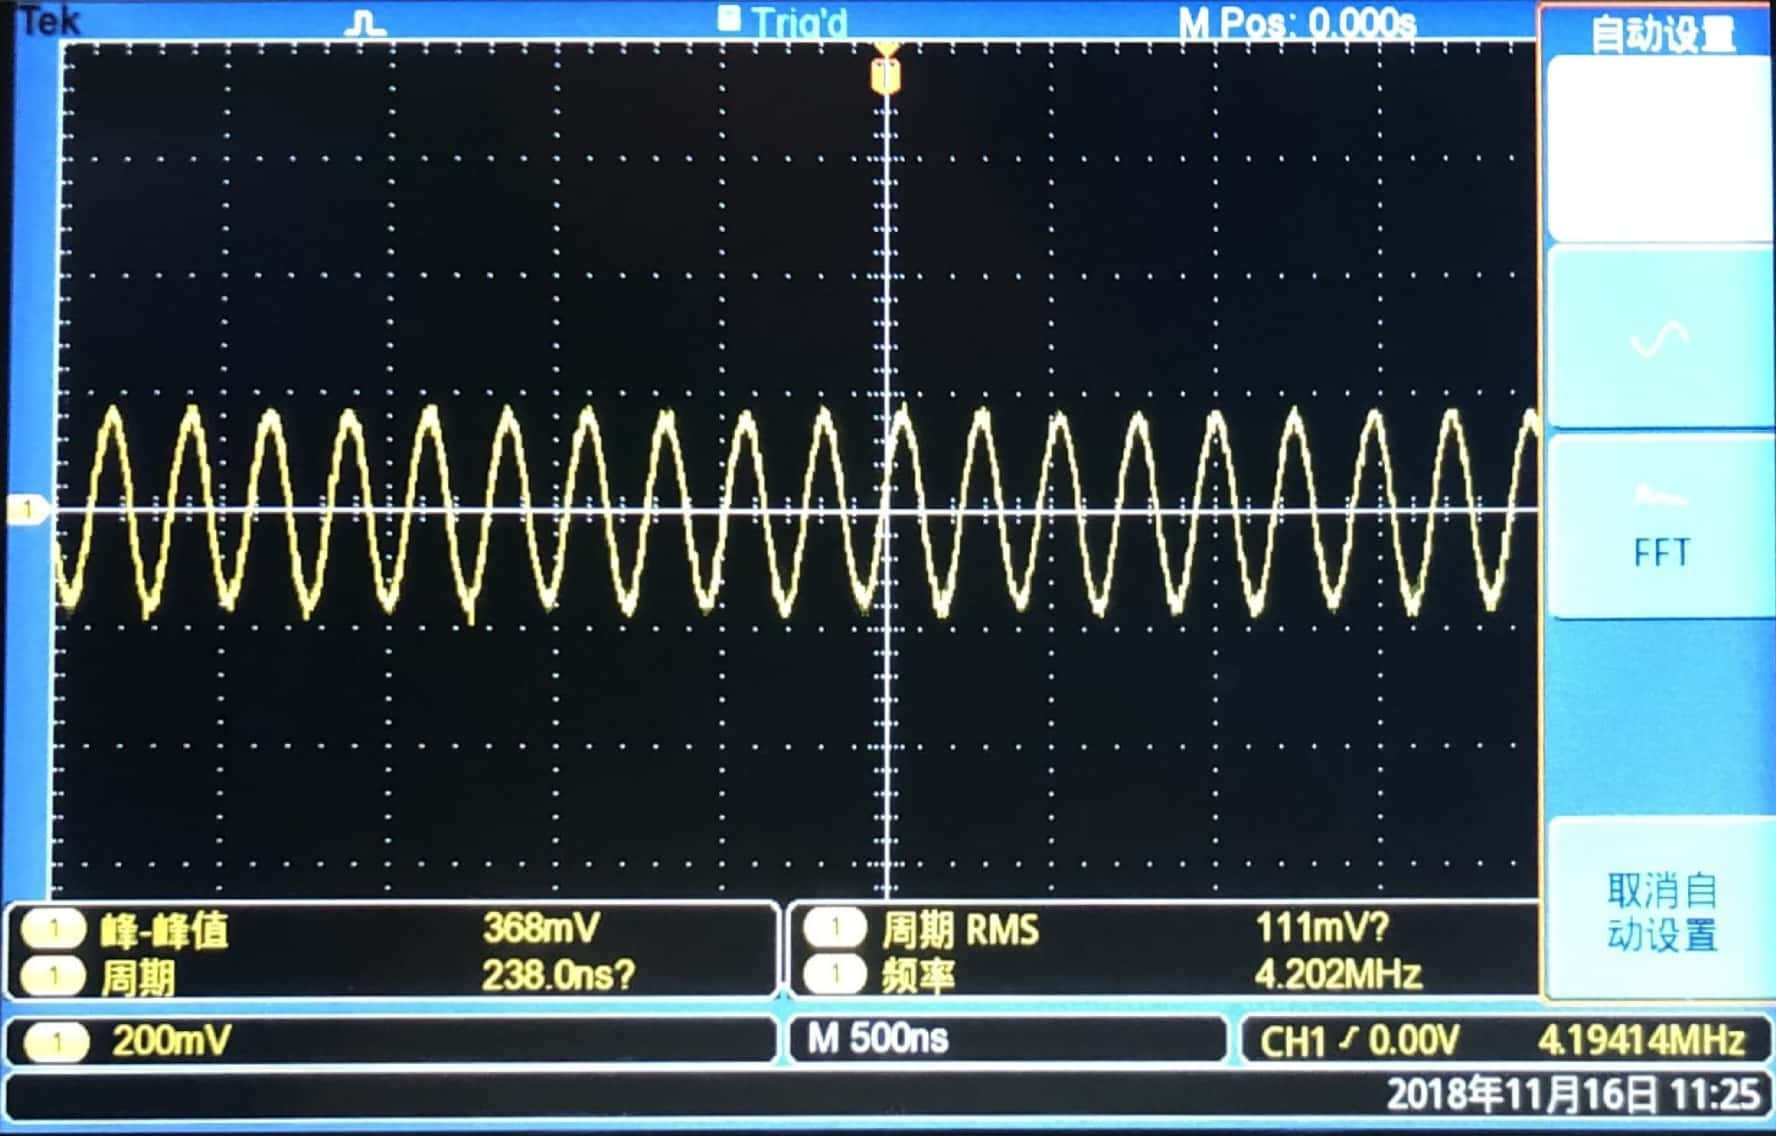
\includegraphics[width=0.5\textwidth]{gaopin1/gaopin114.jpg} 
  \caption{ 皮尔斯振荡电路波形图} 
  \label{img212} 
\end{figure}
\end{enumerate}
\subsection{实验仪器}
\begin{tabular}{clcc}
1. &高频实验箱& & 1台 \\       
2. &双踪示波器     & &    1台\\
3.&万用表    &       & 1块\\
\end{tabular}

\subsection{实验结果补充及分析}
\begin{enumerate}\addtolength{\itemsep}{-1.5ex}
\item 某一时刻,西勒振荡器发射极电流$I_e$、对应点的振荡幅度$V_{P-P}$(峰—峰值)、停振时的静态工作点电流值$I_{eq}$及波形相关情况如表\ref{my-label}所示。
\begin{table}[ht]
\centering
\caption{西勒振荡器相关情况}
\label{my-label}
\begin{tabular}{|c|c|c|c|}
\hline
$I_{eq}(mA)$          & $I_{e}(mA)$           & $V_{P-P}(mv)$ &波形图\\ \hline
1.90& 2.08 & 57.6     &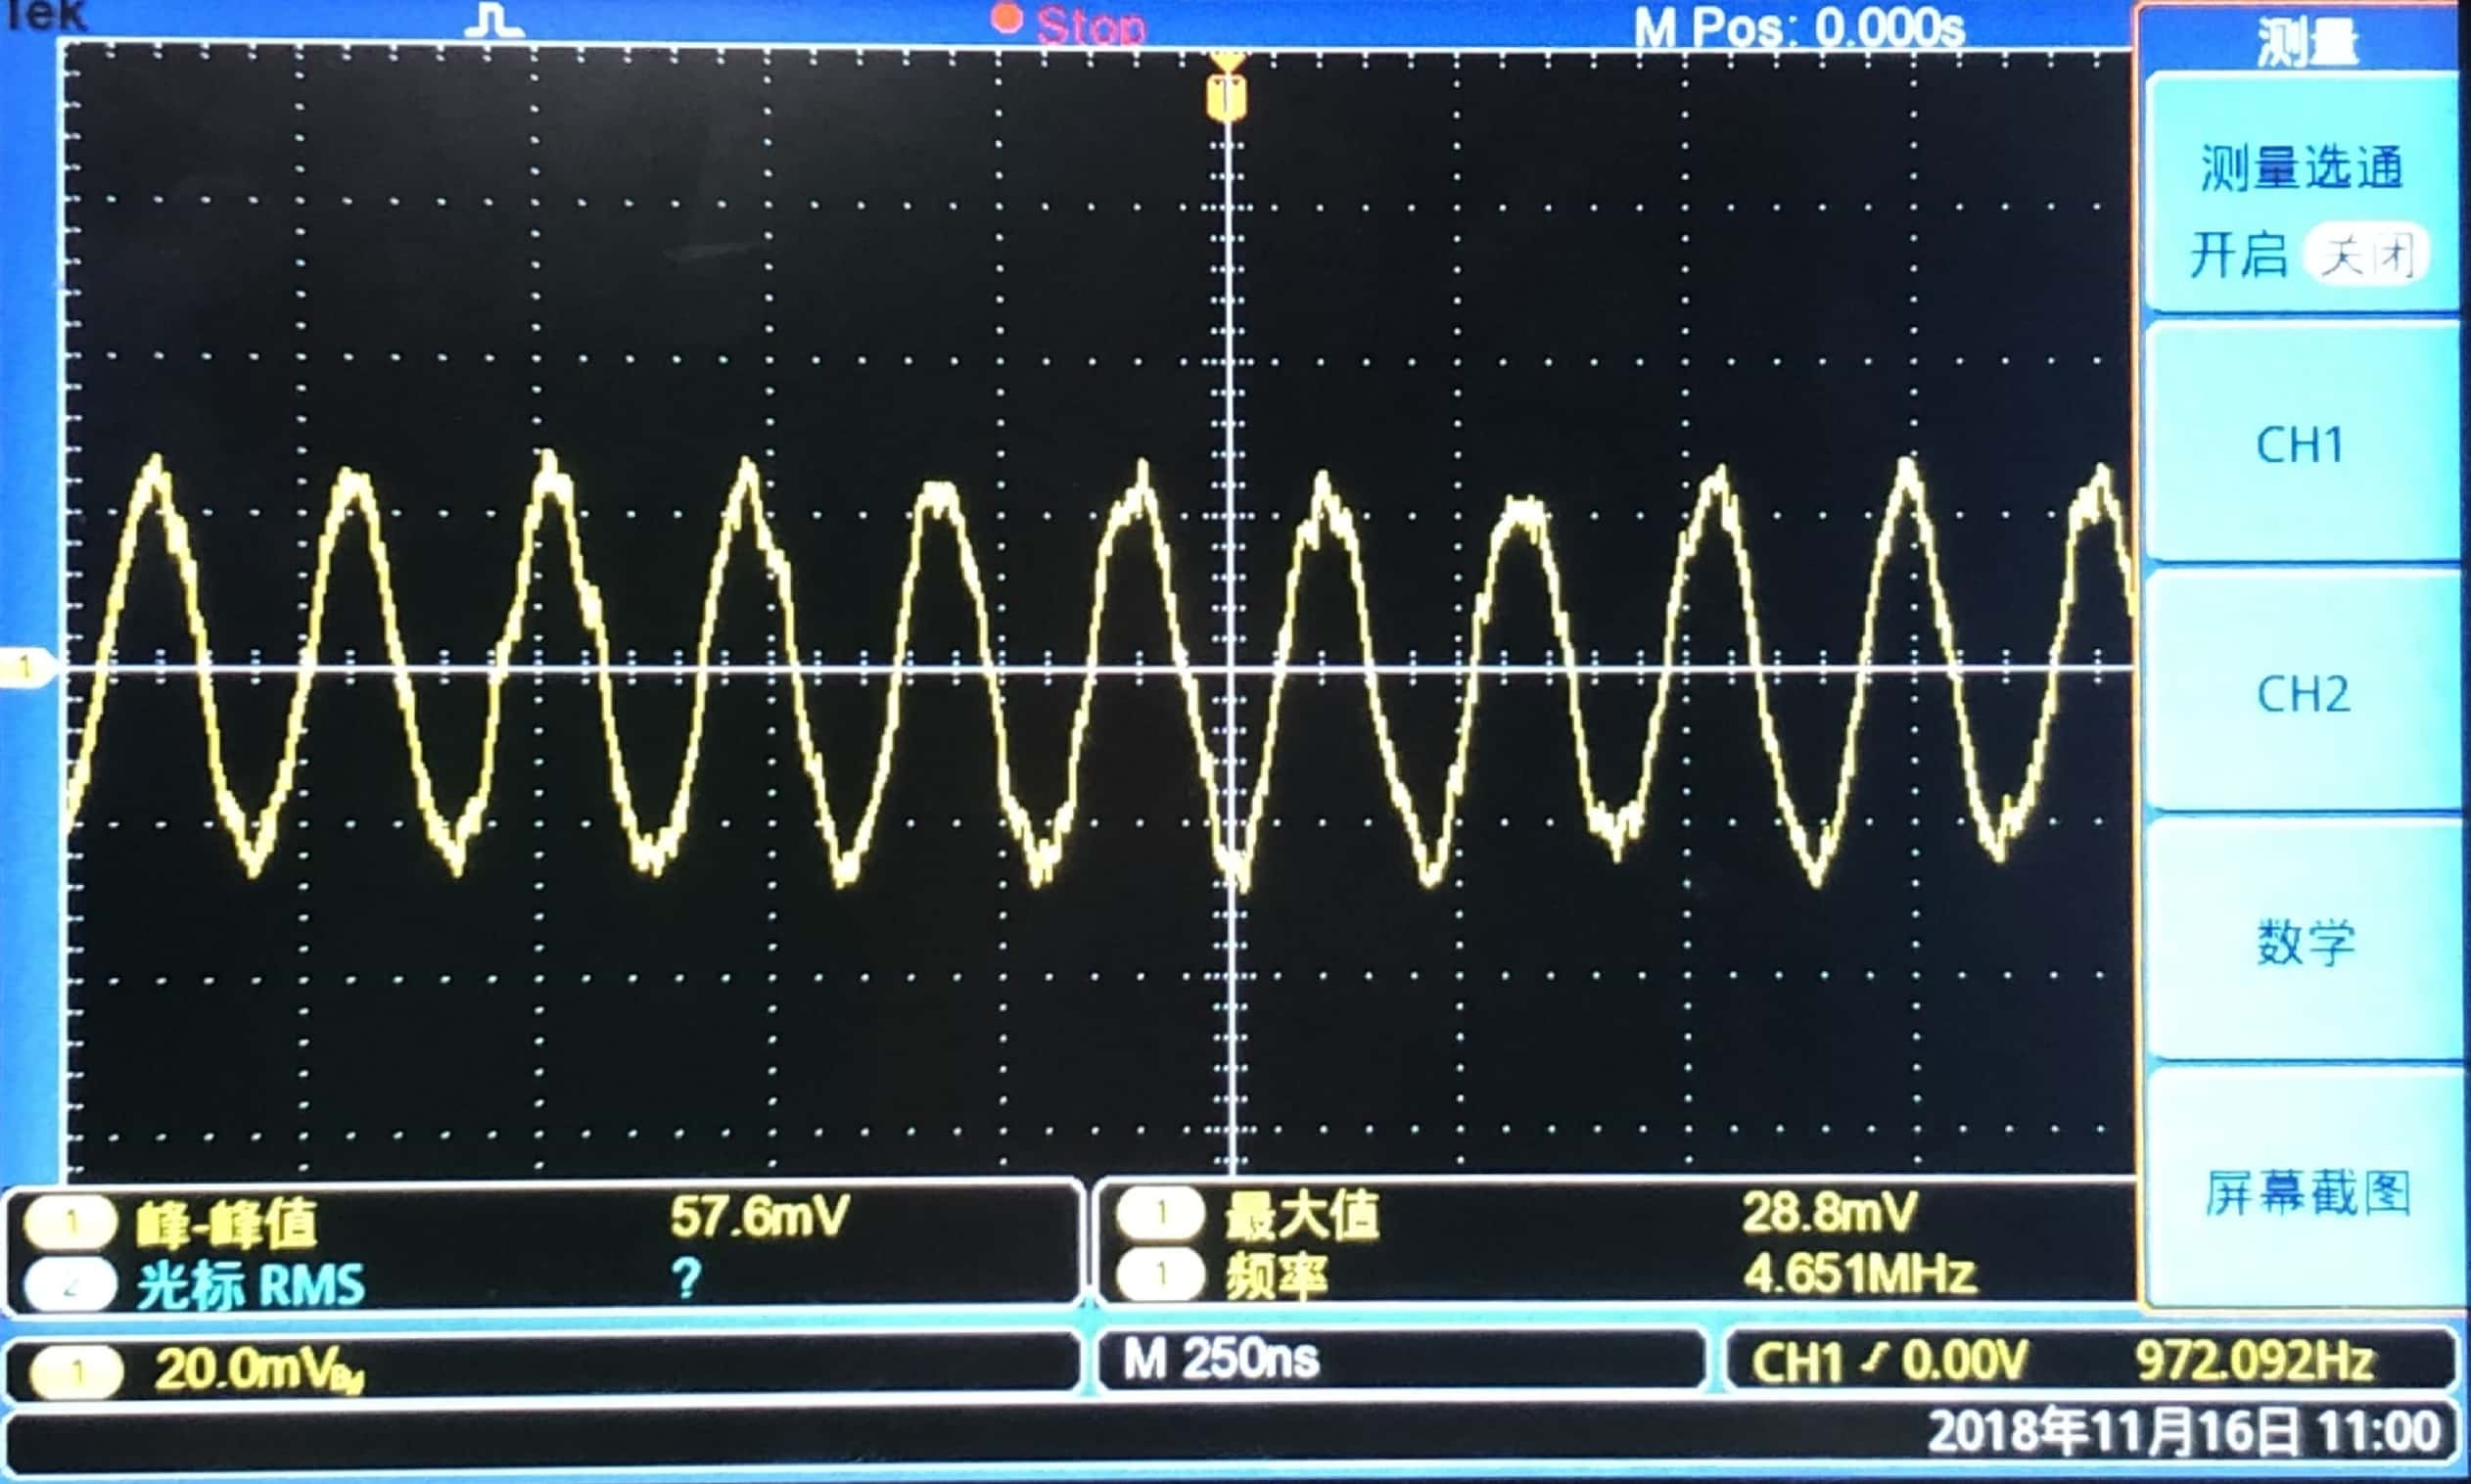
\includegraphics[width=0.4\textwidth]{gaopin1/gaopin106.jpg}     \\  \hline
\end{tabular}
\end{table}
\item 西勒振荡器振荡幅度与静态工作点关系波形图见图\ref{img:12}。
\begin{figure}[ht]
\centering
\label{tab11}
\begin{tabular}{cc}
 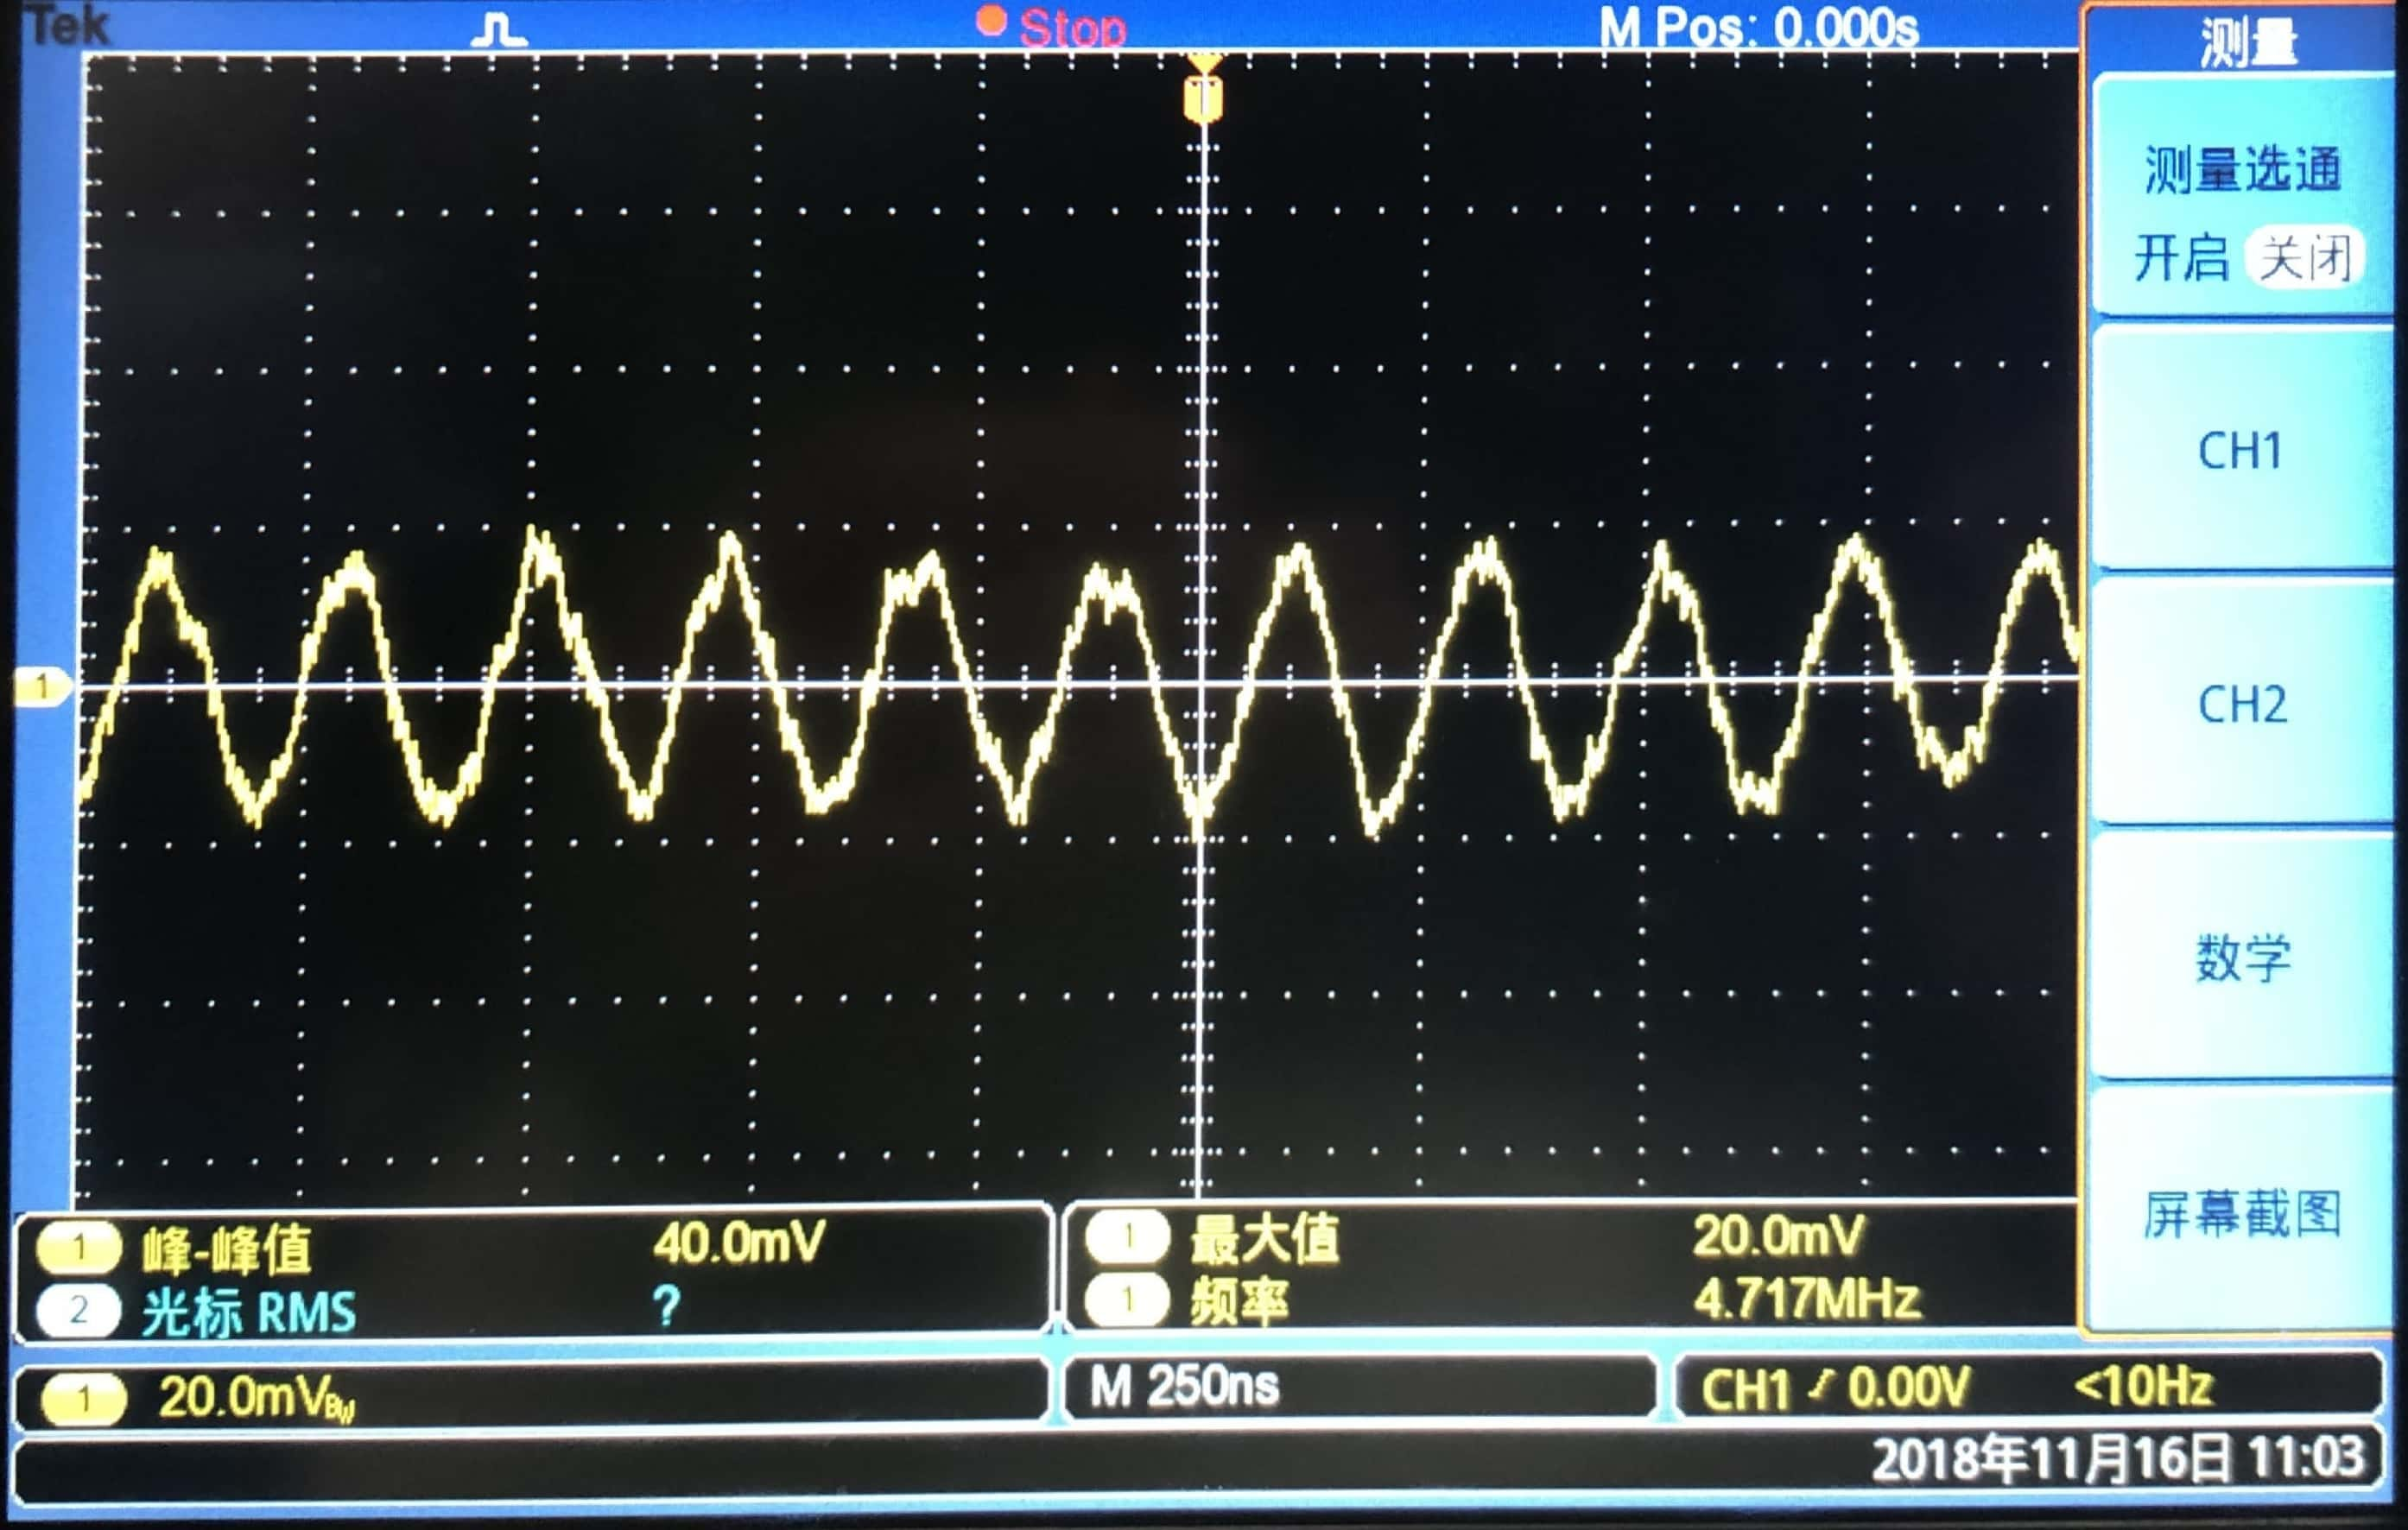
\includegraphics[width=0.4\textwidth]{gaopin1/gaopin103.jpg} &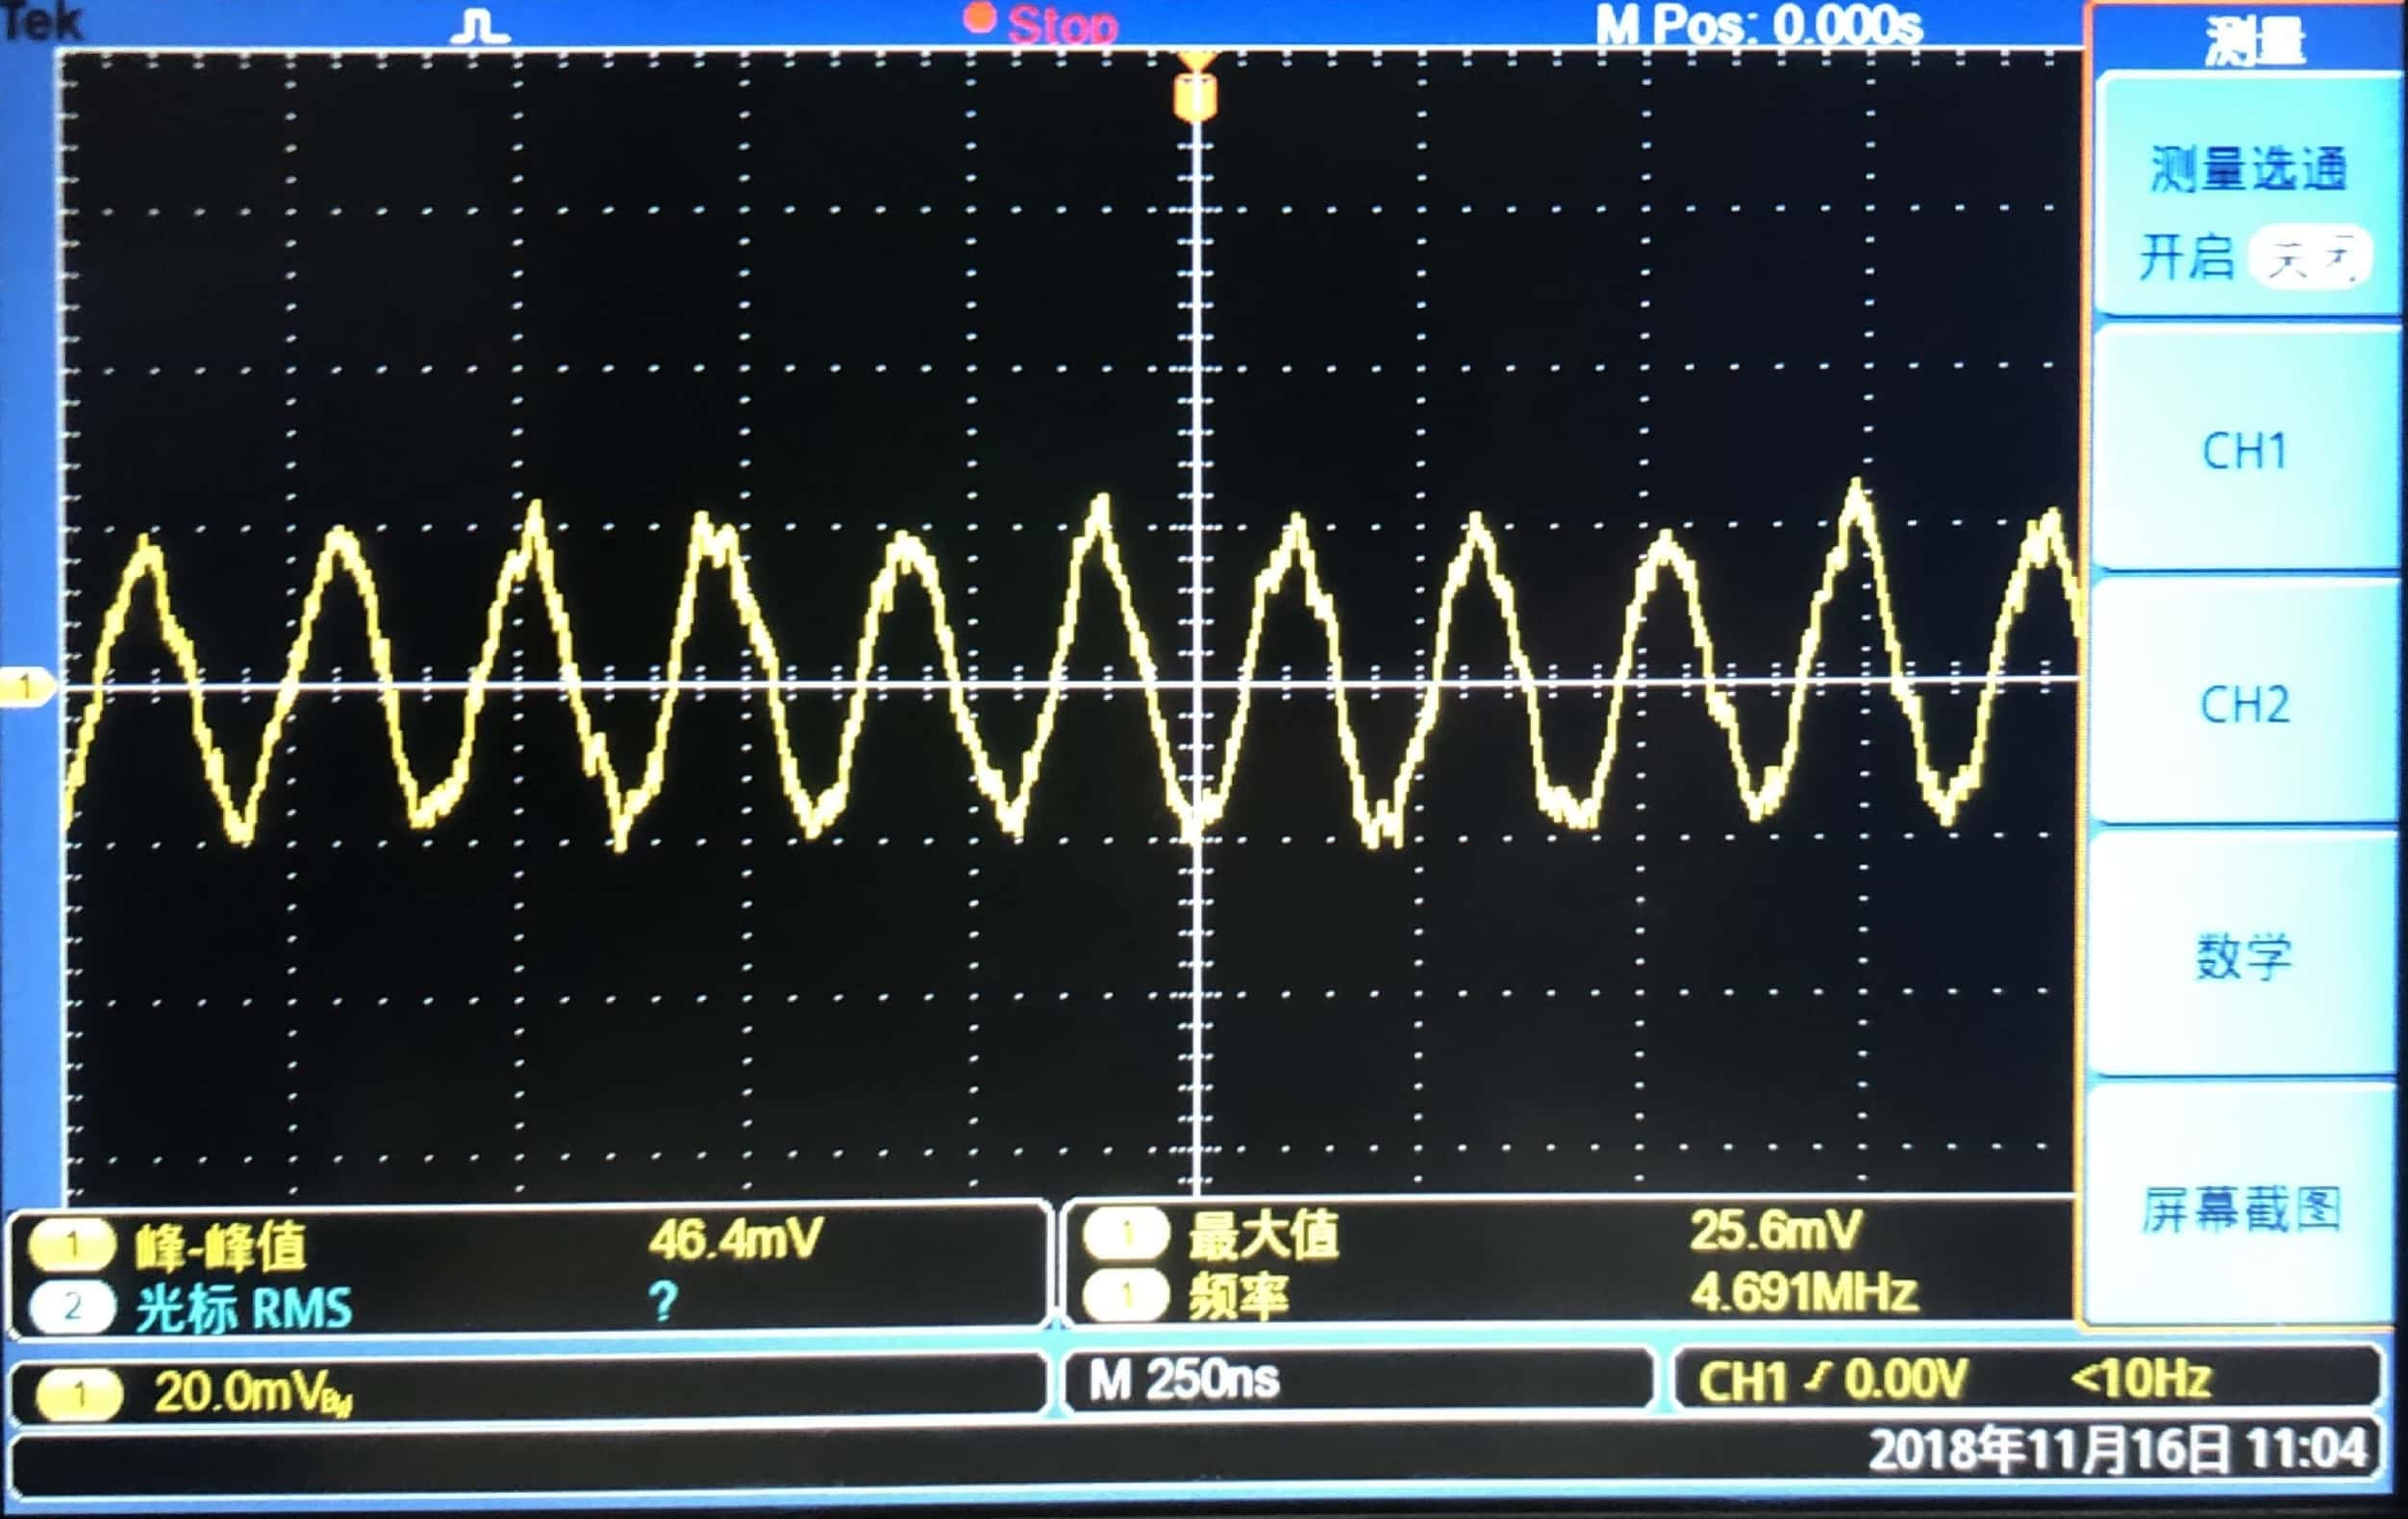
\includegraphics[width=0.4\textwidth]{gaopin1/gaopin102.jpg} \\ 
$I_{eq}=1.2(mA)$  & $I_{eq}=1.4(mA)$  \\
$U_{P-P}=40.0(mv)$ & $U_{P-P}=46.4(mv)$ \\
\\
 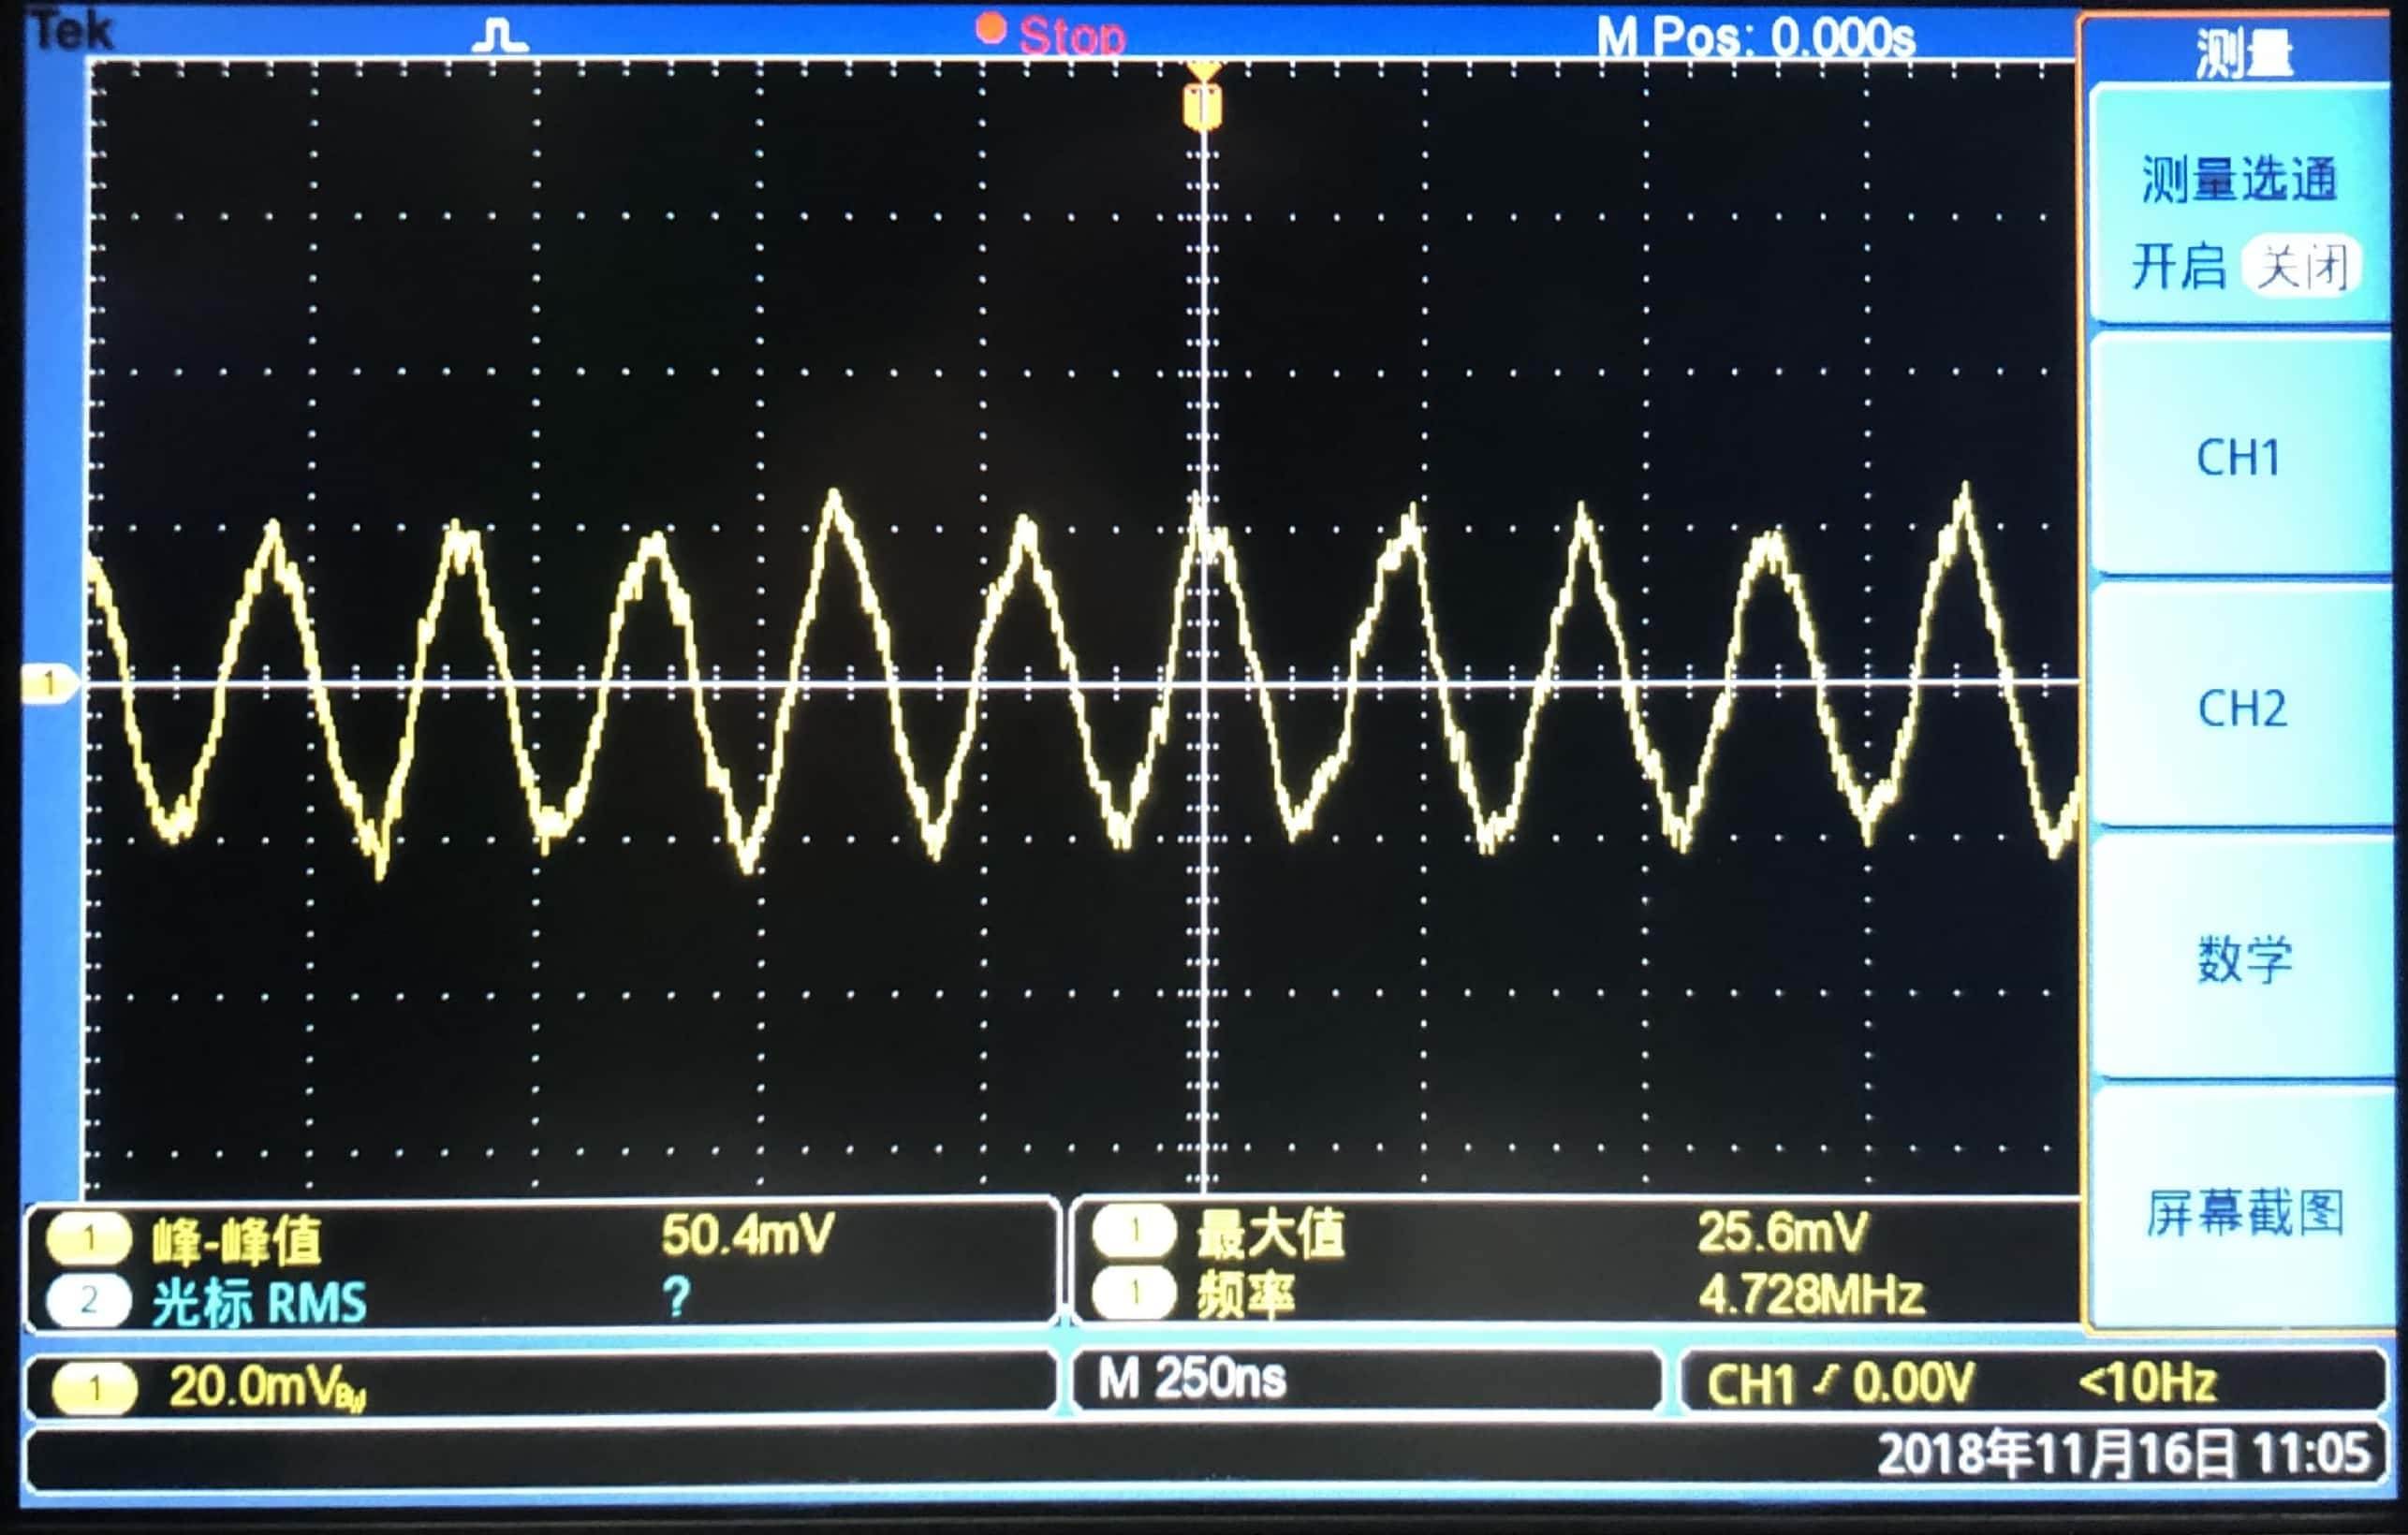
\includegraphics[width=0.4\textwidth]{gaopin1/gaopin109.jpg}&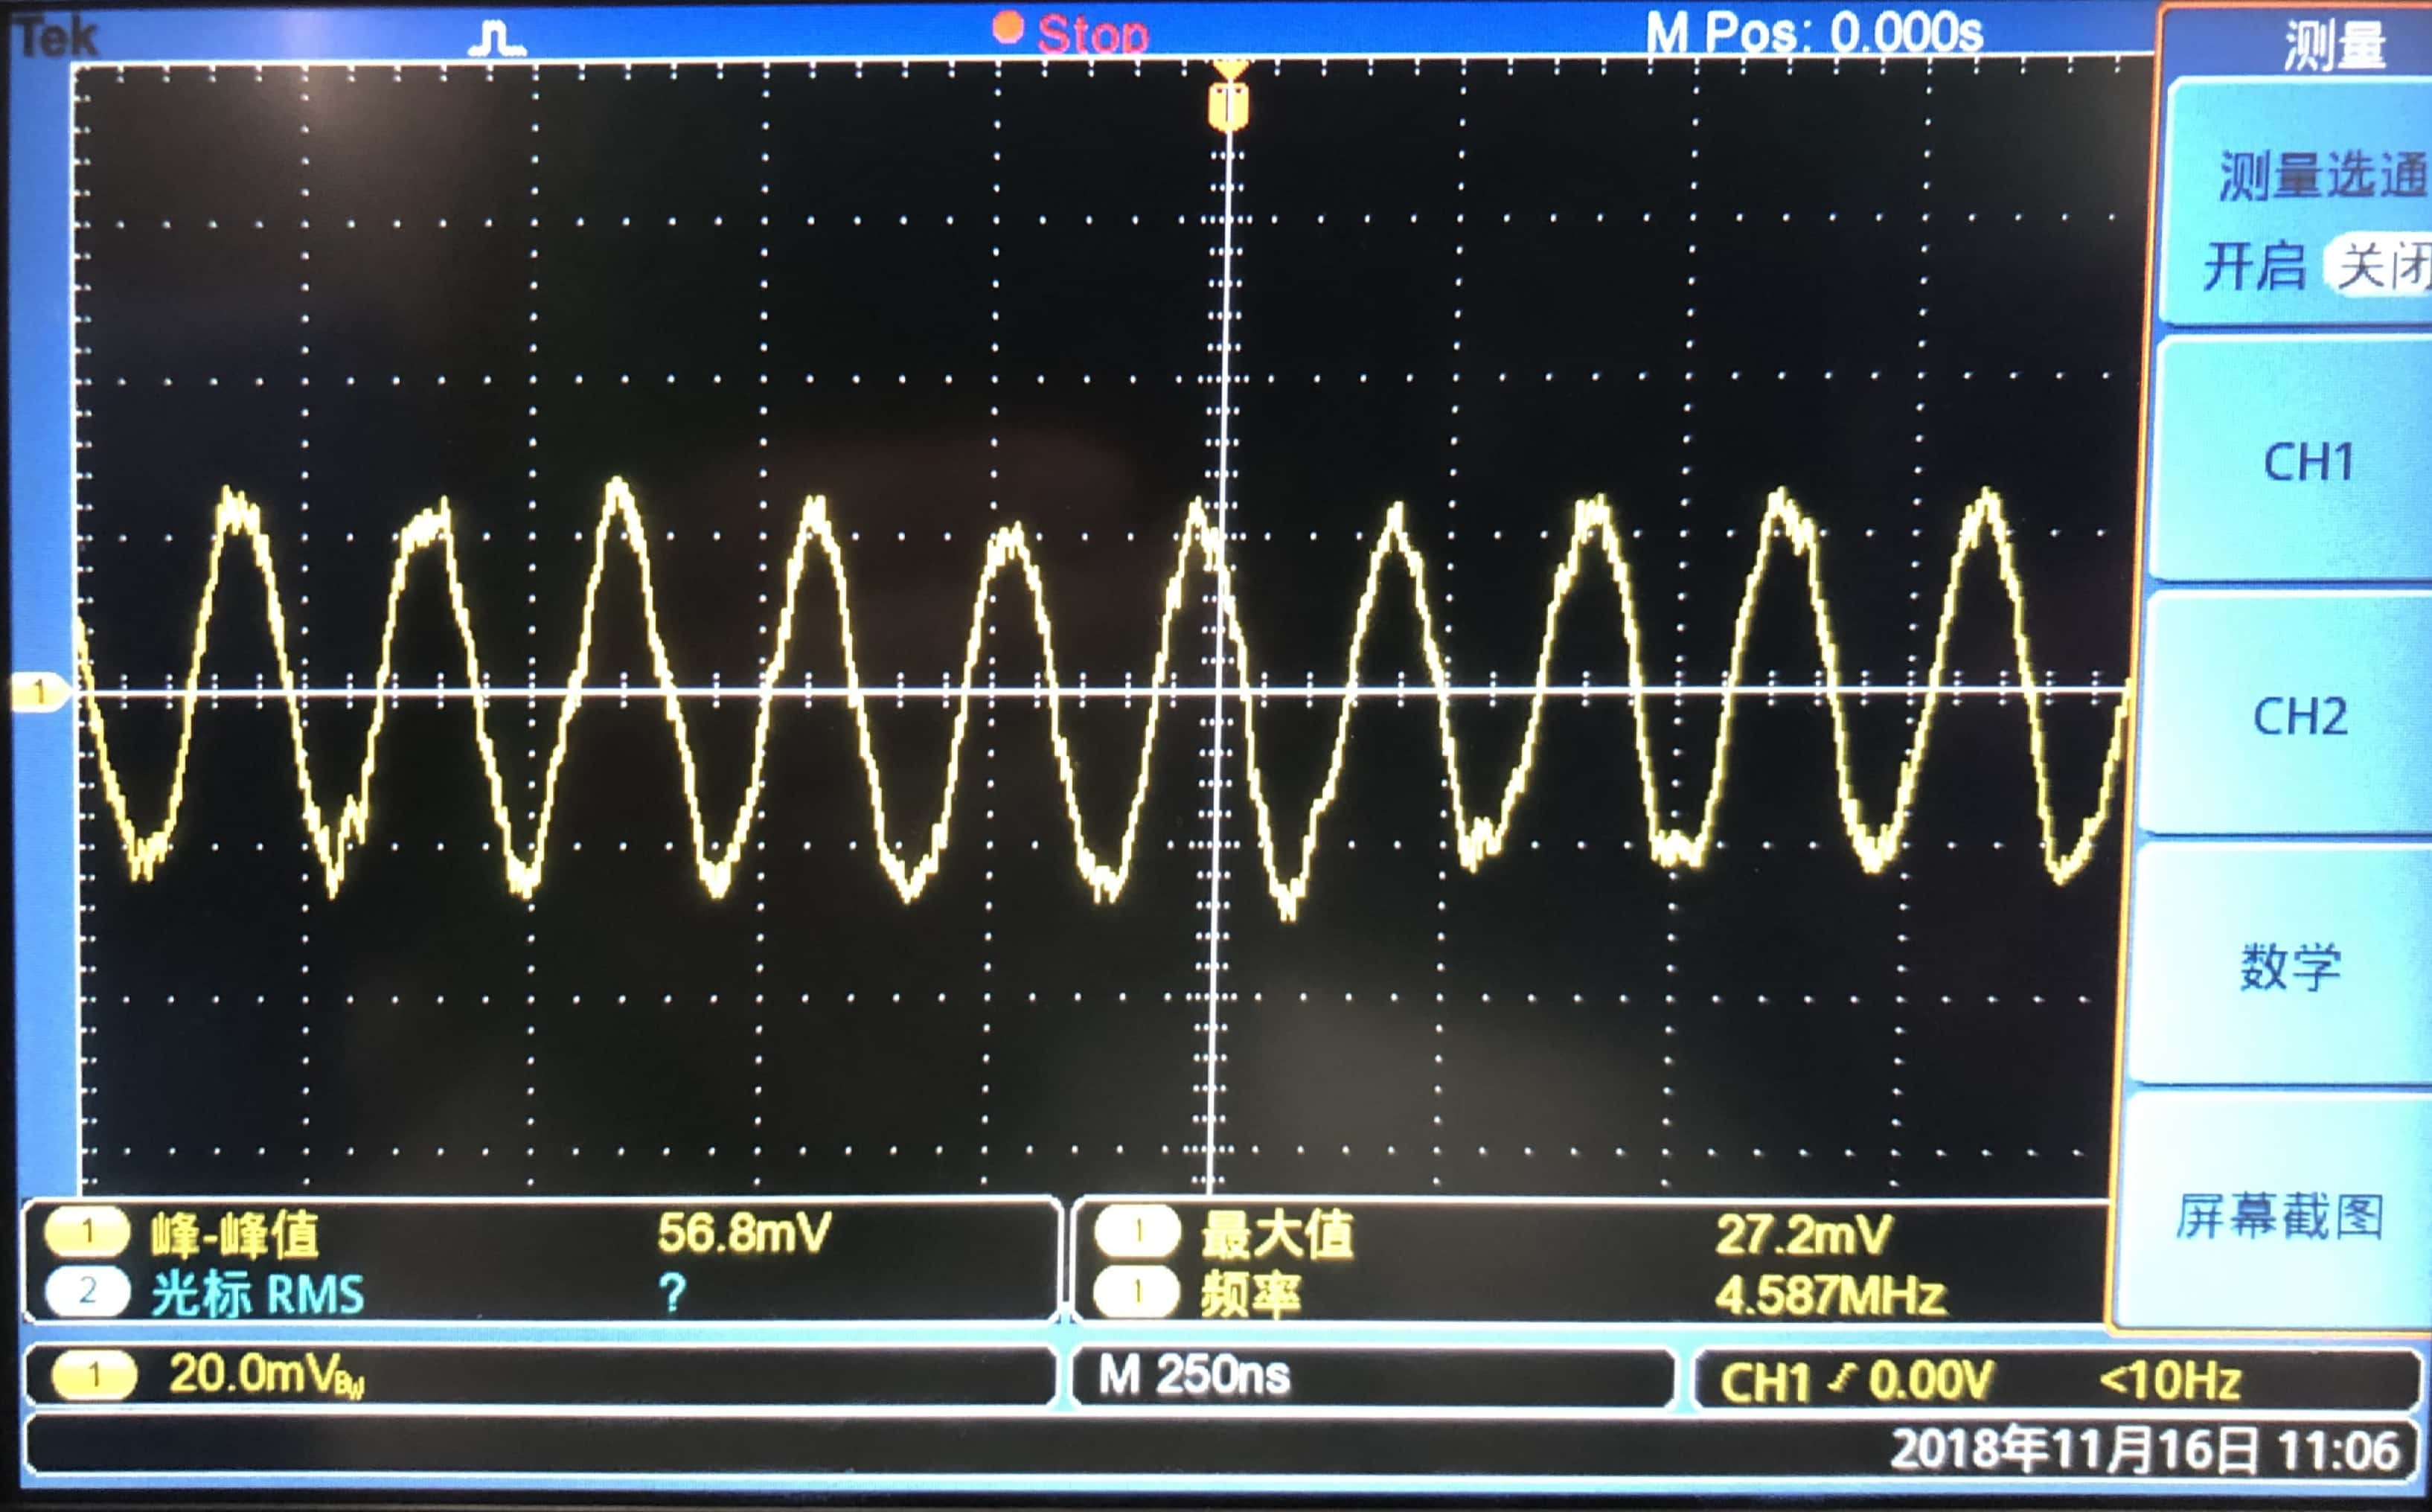
\includegraphics[width=0.4\textwidth]{gaopin1/gaopin107.jpg}  \\ 
$I_{eq}=1.6(mA)$  & $I_{eq}=1.8(mA)$  \\
$U_{P-P}=50.4(mv)$ & $U_{P-P}=56.8(mv)$ \\
\end{tabular}
\caption{振荡幅度与静态工作点关系波形图}\label{img:12}
\end{figure}
\item \emph{分析静态工作点、反馈系数F对振荡器起振条件和输出波形振幅的影响,并用所学理论加以分析。}
\begin{enumerate}[(i)]\addtolength{\itemsep}{-1.5ex}
\item 由实验结果可得:输出波形$V_{P-P}$ 的峰值随着$I_{eq}$ 的增加而增加。\par
理论分析如下:
静态工作点主要影响振荡器的起振条件,晶体管起振时要求$V_{be}$ 为负偏压状
态,此后加上正反馈后才可起振,此时放大器处于线性放大状态;当幅度增加到
一定值时放大器进入非线性平衡状态。\par
在此次实验中,LC 电路产生的振荡信号经由射极跟随器、谐调放大器与滤
波最终到达输出端,因此输出波形应随着LC 振荡器产生的振荡信号的变化而变
化。
\item 反馈系数F 对振荡器起振条件和输出波形振幅的影响:\par
理论分析如下:振荡器的起振条件要求:$ A_{oF}>1$ ,要维持一定振幅的振荡,反馈系
数F 要设计的比$A_{oF}=1$ 中的F 大一些,一般取$F=\frac{1}{2}\sim\frac{1}{8}$,这样,就可以使得$A_{oF}>1$的情况下起振,而后随着振幅增强$A_o$就向 A 过渡, 直到振幅增大某一程度出现$ A_F=1 $时,振幅就达到平衡状态,反馈系数 F对振荡幅度的大小没有影响。 
\end{enumerate}
\end{enumerate}
\section{高频小信号调谐放大器实验(模块3)}
\setcounter{equation}{0}
\setcounter{table}{0}
\setcounter{figure}{0}
\subsection{实验目的}
\begin{enumerate}\addtolength{\itemsep}{-1.5ex}
\item 掌握小信号调谐放大器的基本工作原理;
\item 掌握谐振放大器电压增益、通频带、选择性的定义、测试及计算;
\end{enumerate}
\subsection{实验原理}
 \begin{figure}[ht]
  \centering
  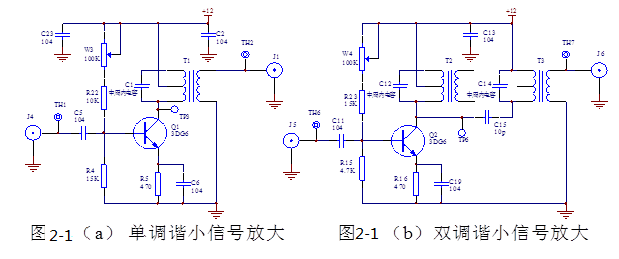
\includegraphics[width=\textwidth]{image006.png} 
  \caption{ 实验原理} 
  \label{img21111} 
\end{figure}
原理图如图\ref{img21111}所示。
\begin{enumerate}\addtolength{\itemsep}{-1.5ex}
\item 单调谐放大器\par
   小信号谐振放大器是通信机接收端的前端电路,主要用于高频小信号或微弱信号的线性放大。其实验单元电路如图\ref{img21111}(a)所示。该电路由晶体管$Q_1$、选频回路$T_1$二部分组成。它不仅对高频小信号进行放大,而且还有一定的选频作用。本实验中输入信号的频率$f_S=12MHz$。基极偏置电阻$W_2,R_1,R_2$和射极电阻$R_3$决定晶体管的静态工作点。可变电阻$W_2$改变基极偏置电阻将改变晶体管的静态工作点,从而可以改变放大器的增益。表征高频小信号调谐放大器的主要性能指标有谐振频率$f_0$,谐振电压放大倍数$A_{v0}$,放大器的通频带$B_W$及选择性(通常用矩形系数$K_{r0.1}$来表示)等。
\item 双调谐放大器\par
    双调谐放大器具有频带较宽、选择性较好的优点。双调谐回路谐振放大器是将单调谐回路放大器的单调谐回路改用双调谐回路。其原理基本相同。
    \end{enumerate}
\subsection{实验步骤}
\subsubsection{单调谐小信号放大器单元电路实验}
\begin{enumerate}[1.]\addtolength{\itemsep}{-1.5ex}
\item 根据电路原理图熟悉实验板电路,并在电路板上找出与原理图相对应的的各测试点及可调器件(具体指出)。
\item 按框图\ref{img22}所示搭建好测试电路。
  \begin{figure}[ht]
  \centering
  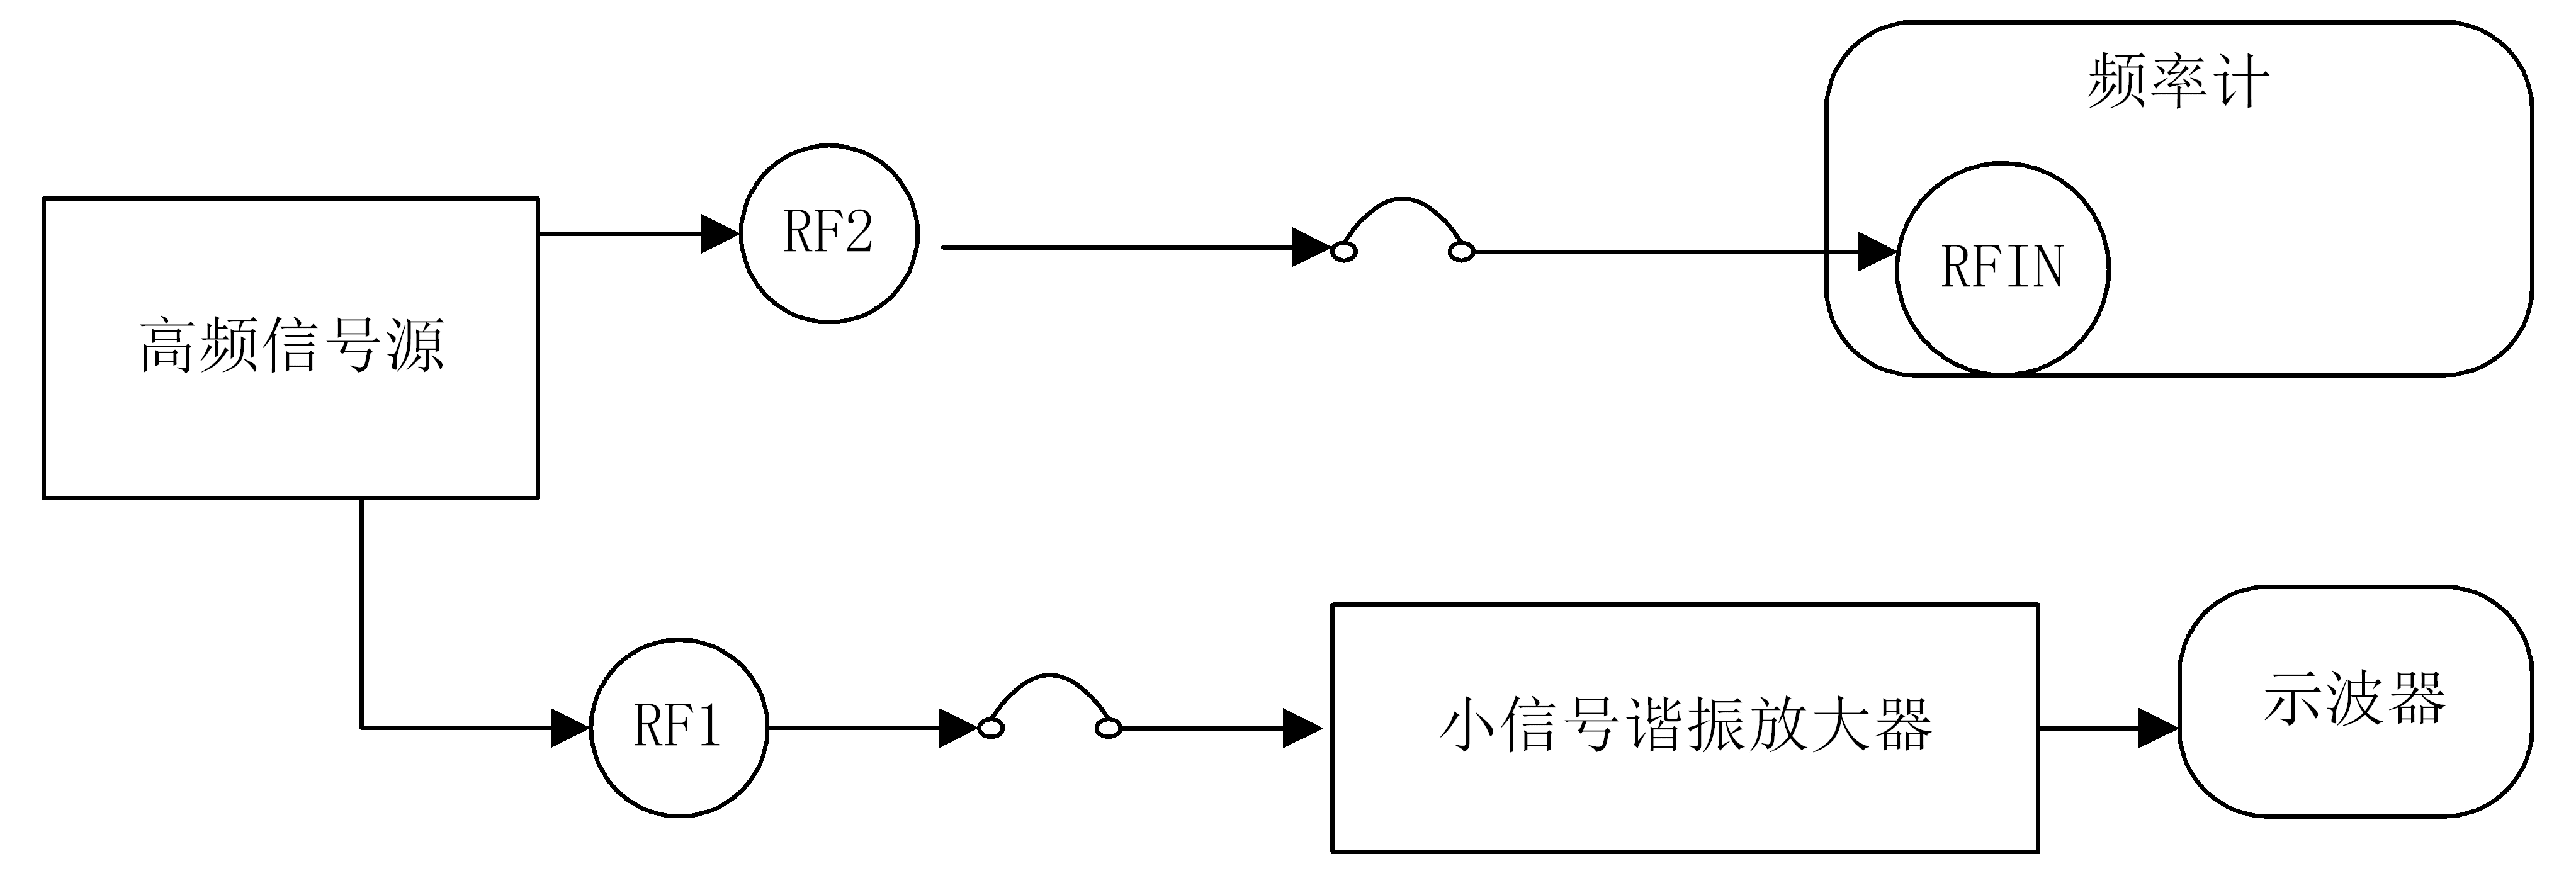
\includegraphics[width=\textwidth]{image000.png} 
  \caption{ 高频小信号调谐放大器测试连接框图} 
  \label{img22} 
\end{figure}
\item 打开小信号调谐放大器的电源开关,并观察工作指示灯是否点亮,红灯为+12V电源指示灯,绿灯为-12V电源指示灯。(以后实验步骤中不再强调打开实验模块电源开关步骤)
\item 调整晶体管的静态工作点;
\item 测量电压增益Av0\par
在调谐放大器对输入信号已经谐振的情况下,用示波器探头在TH1和TH2分别观测输入和输出信号的幅度大小,如表\ref{my-label1:a}所示,则Av0即为输出信号与输入信号幅度之比,由式(\ref{g:1})知,为25.14。
\begin{table}[htbp]
\centering
\caption{单调谐放大器输出信号与输入信号关系}
\label{my-label1:a}
\begin{tabular}{|c|c|c|c|}
\hline
      & 频率$(MHz)$ & 幅度$(V)$ & 波形图 \\ \hline
$V_i$ & 12        & 0.105   &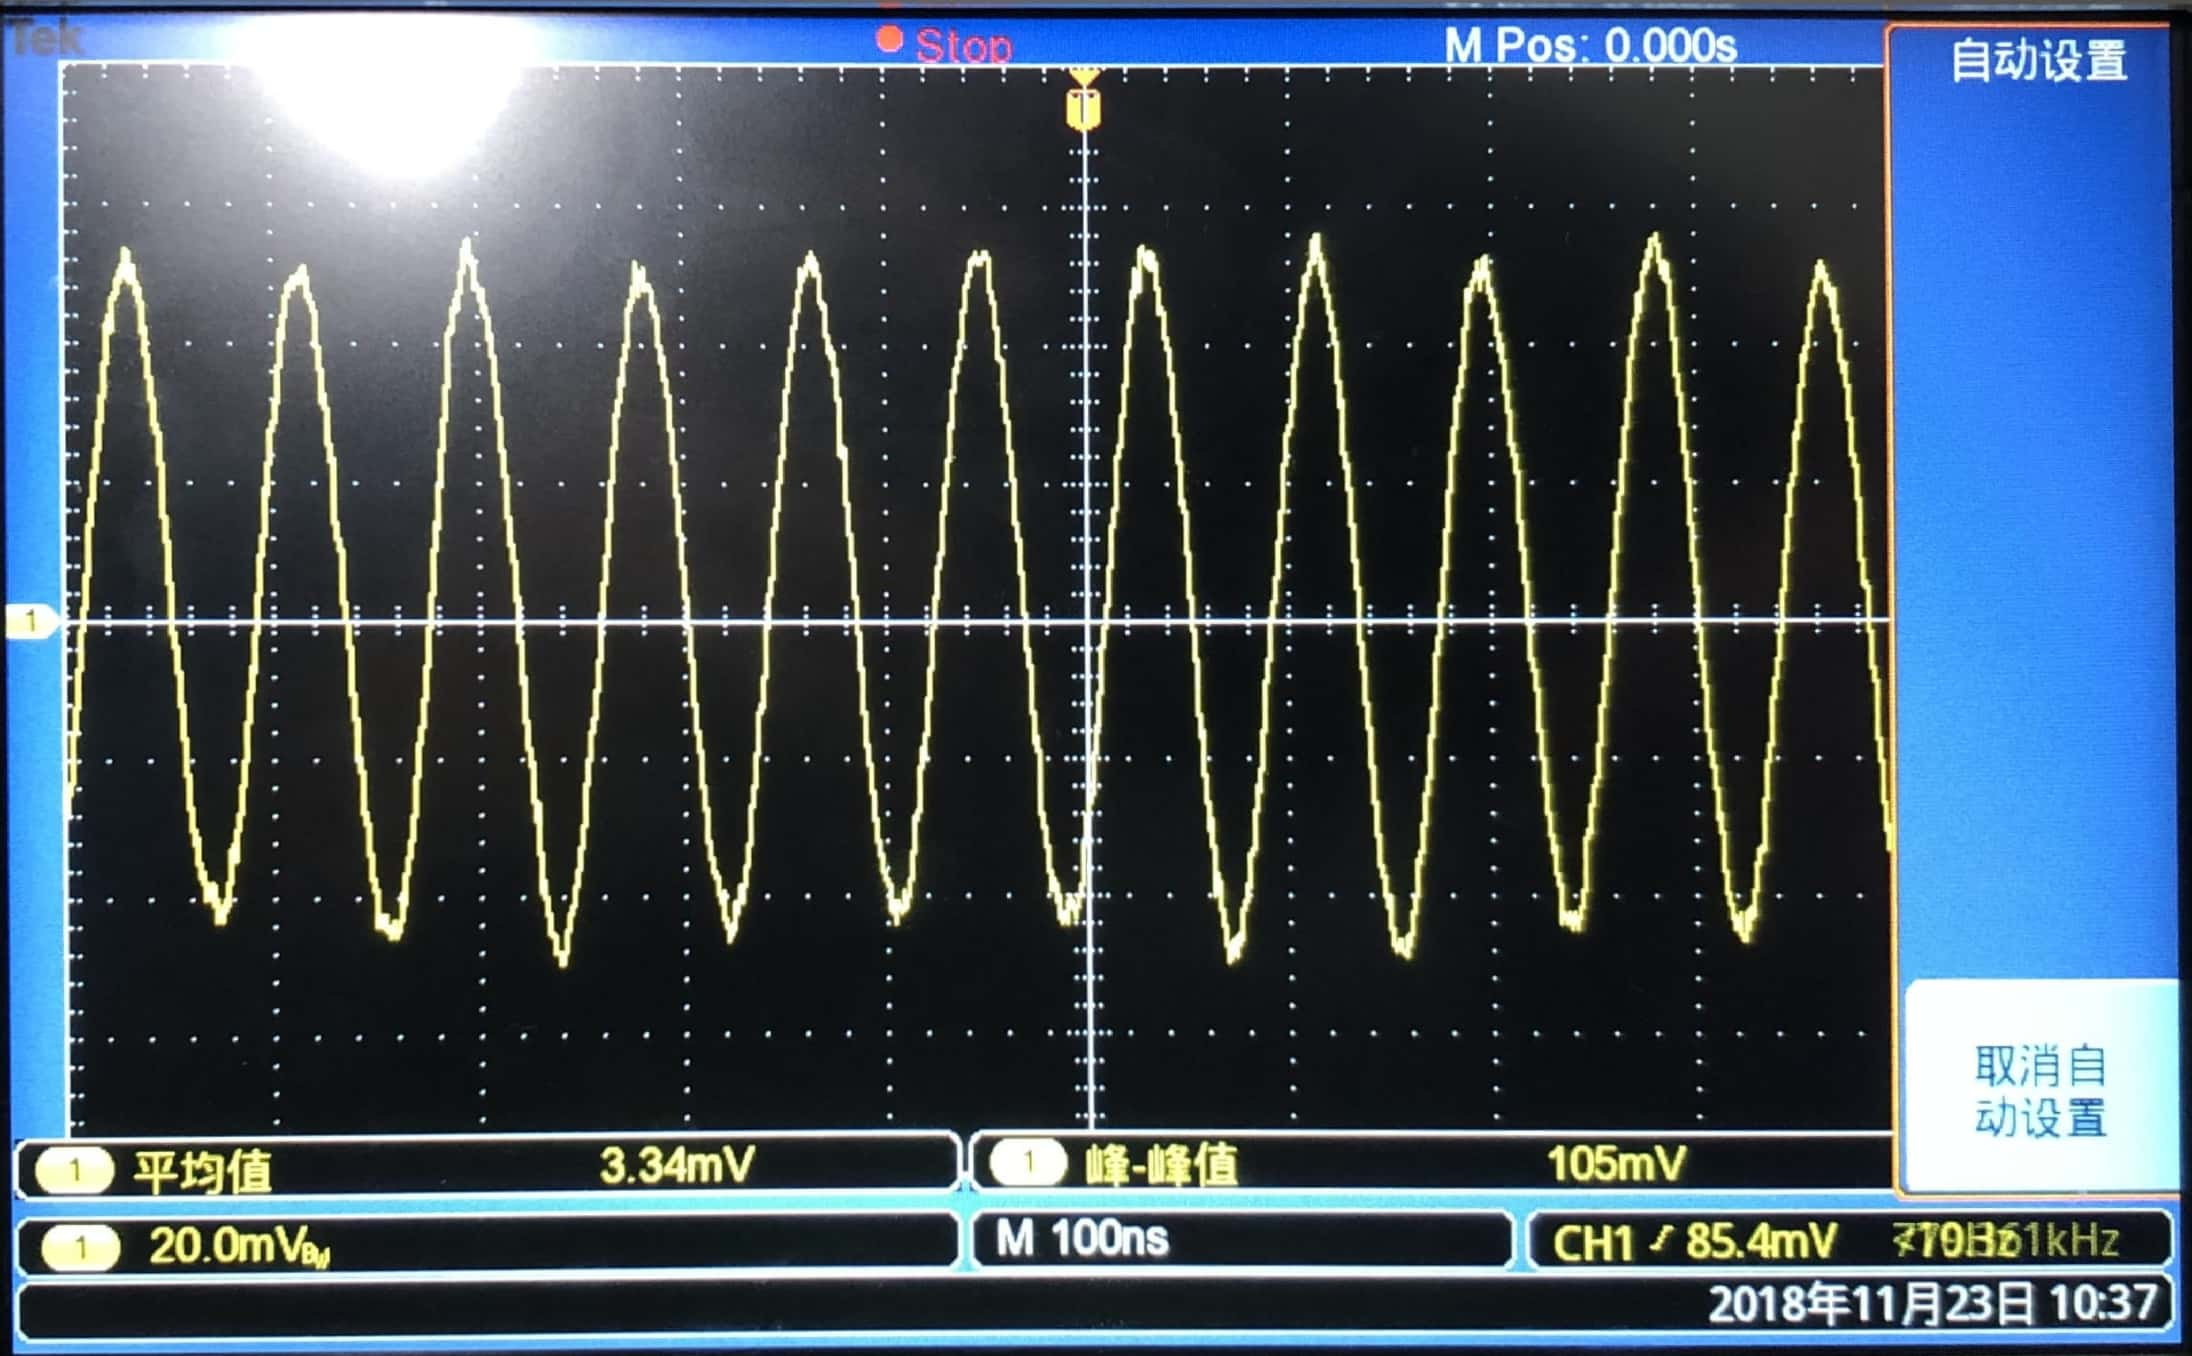
\includegraphics[width=0.35\textwidth]{gaopin2/gaopin209.jpg}    \\ \hline
$V_o$ & 12        & 2.64    & 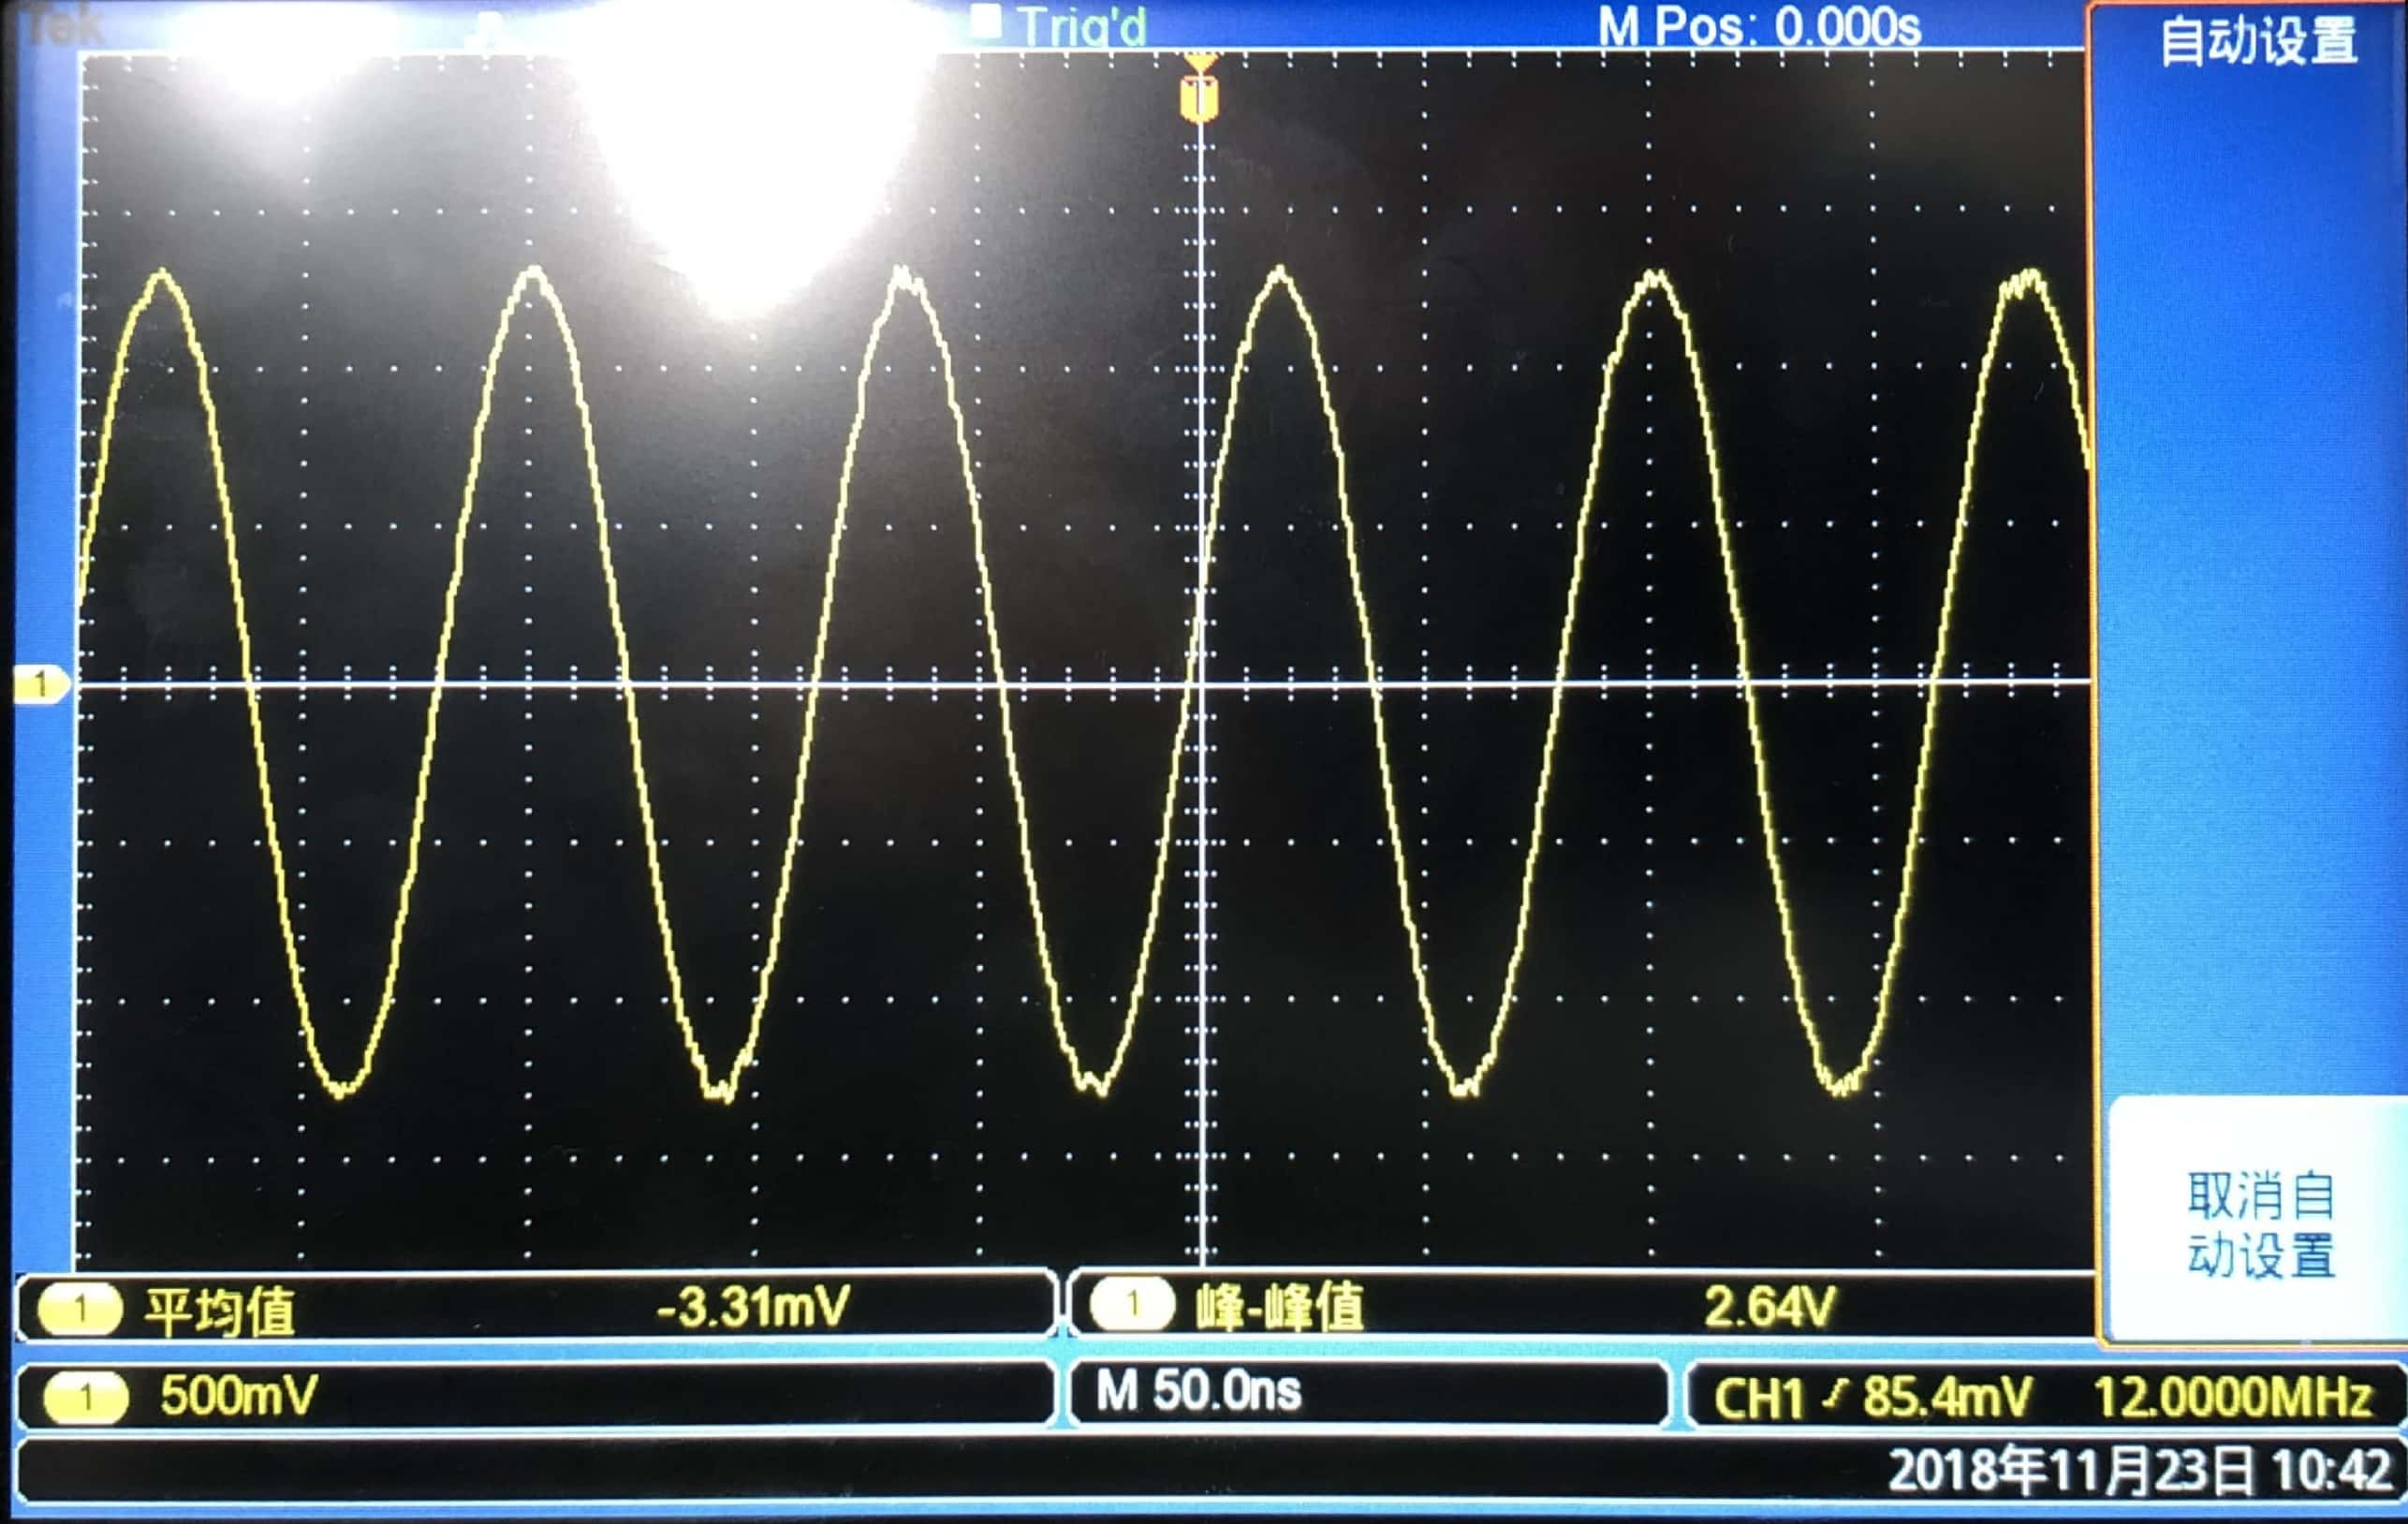
\includegraphics[width=0.35\textwidth]{gaopin2/gaopin208.jpg}   \\ \hline
\end{tabular}
\end{table}
\begin{equation}\label{g:1}
A_{v0}=\frac{V_{o}}{V_i}=\frac{2.64v}{105mv}=25.14
\end{equation}
\item 测量放大器通频带
   对放大器通频带的测量有两种方式,\par
 其一是用频率特性测试仪(即扫频仪)直接测量;\par
 其二则是用点频法来测量:即用高频信号源作扫频源,然后用示波器来测量各个频率信号的输出幅度,最终描绘出通频带特性,具体方法如下:\par
通过调节放大器输入信号的频率,使信号频率在谐振频率附近变化(以0.2MHz为步进间隔来变化),并用示波器观测各频率点的输出信号的幅度,见表\ref{tab:b},然后就可以在如图\ref{img:c}的“幅度-频率”坐标轴上标示出放大器的通频带特性。
\begin{table}[htbp]
\centering
\caption{单调谐放大器幅度-频率关系}
\label{tab:b}
\begin{tabular}{|c|c|}
\hline
输入频率$(MHz)$ & 输出幅度$(V)$ \\ \hline
11.2        & 1.52      \\ \hline
11.4        & 1.78      \\ \hline
11.6        & 2.26      \\ \hline
11.8        & 2.56      \\ \hline
12          & 2.64      \\ \hline
12.2        & 2.38      \\ \hline
12.4        & 2.10      \\ \hline
12.6        & 1.80      \\ \hline
12.8        & 1.58      \\ \hline
\end{tabular}
\end{table}

    \end{enumerate}
\subsubsection{双调谐小信号放大器单元电路实验}
双调谐小信号放大器的测试方法和测试步骤与单调谐放大电路基本相同,只是在以下两个方面稍作改动:\par
其一是.调节信号源“RF幅度”和“频率调节”旋钮,使输出端口“RF1”和“RF2”输出频率为465KHz(峰-峰值200mV)。将信号输入到3号板的J6口TH9处测试观察,输出在J7口TH10处测试观察。其数据见表\ref{my-label1:ad},同时由式(\ref{g:1e}),电压增益为24.07。\par
\begin{table}[htbp]
\centering
\caption{双调谐放大器输出信号与输入信号关系}
\label{my-label1:ad}
\begin{tabular}{|c|c|c|c|}
\hline
      & 频率$(KHz)$ & 幅度$(V)$ & 波形图 \\ \hline
$V_i$ & 465       & 0.236   &  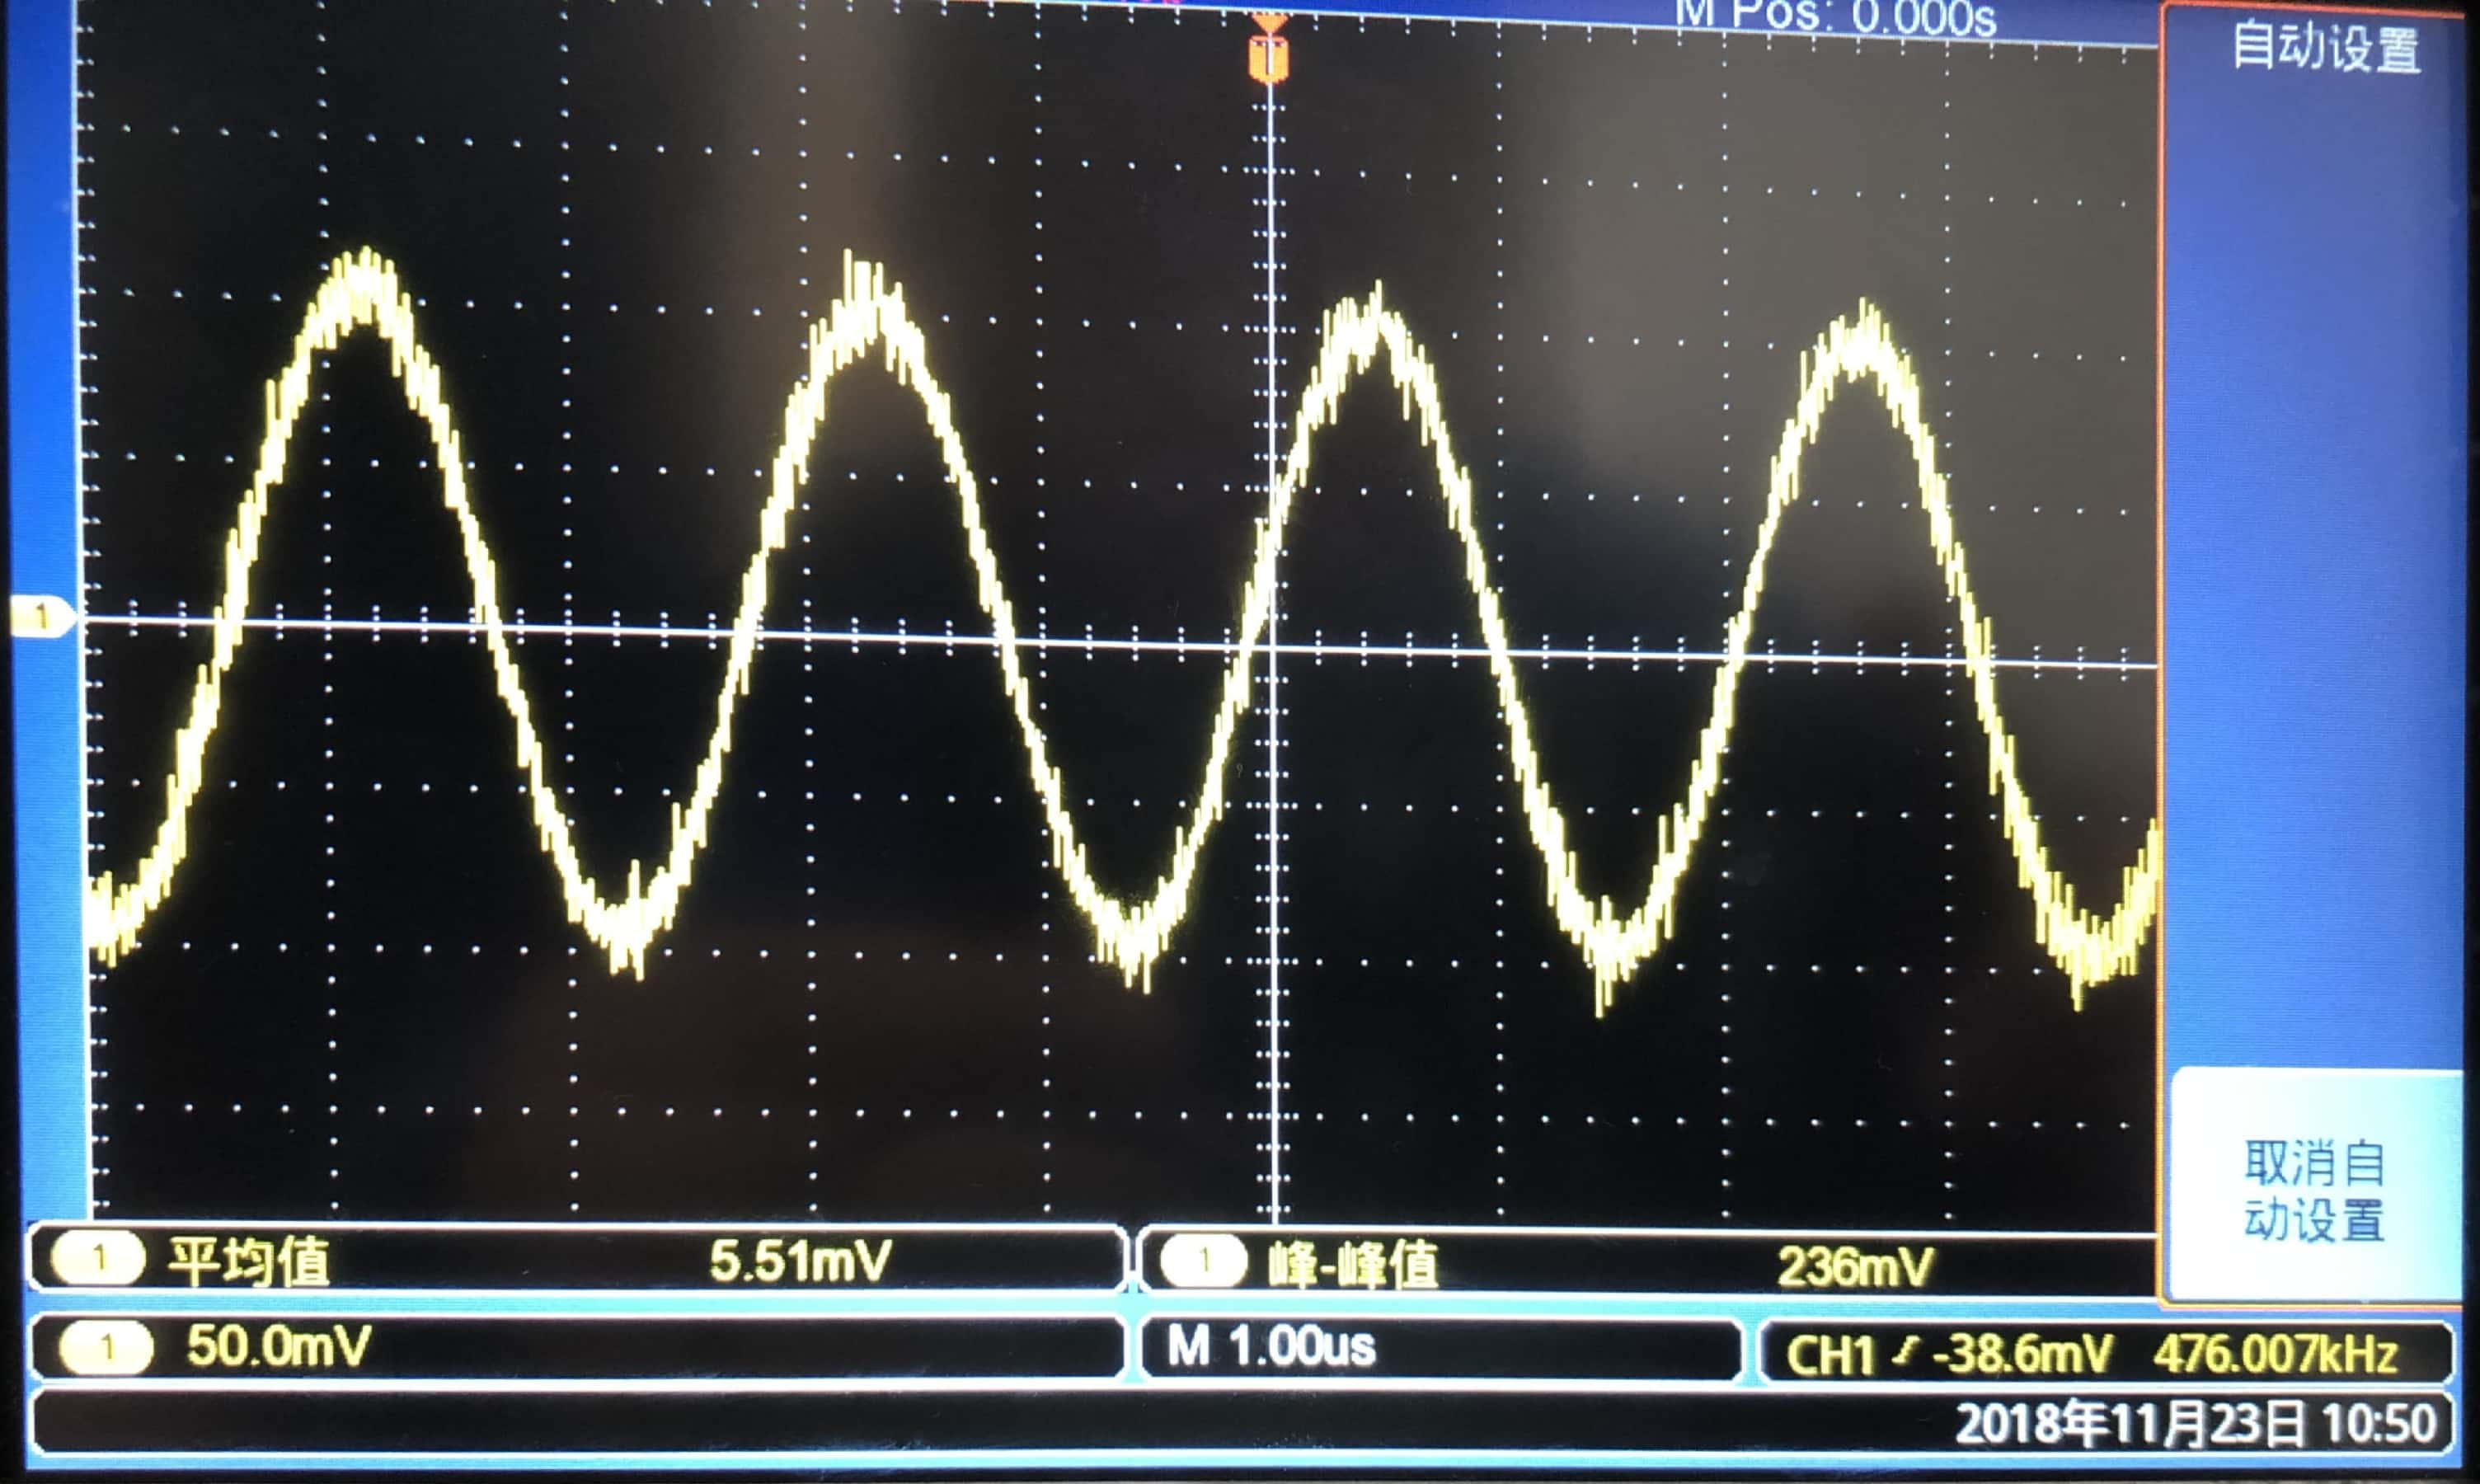
\includegraphics[width=0.35\textwidth]{gaopin2/gaopin215.jpg}   \\ \hline
$V_o$ & 465.001   & 5.68    & 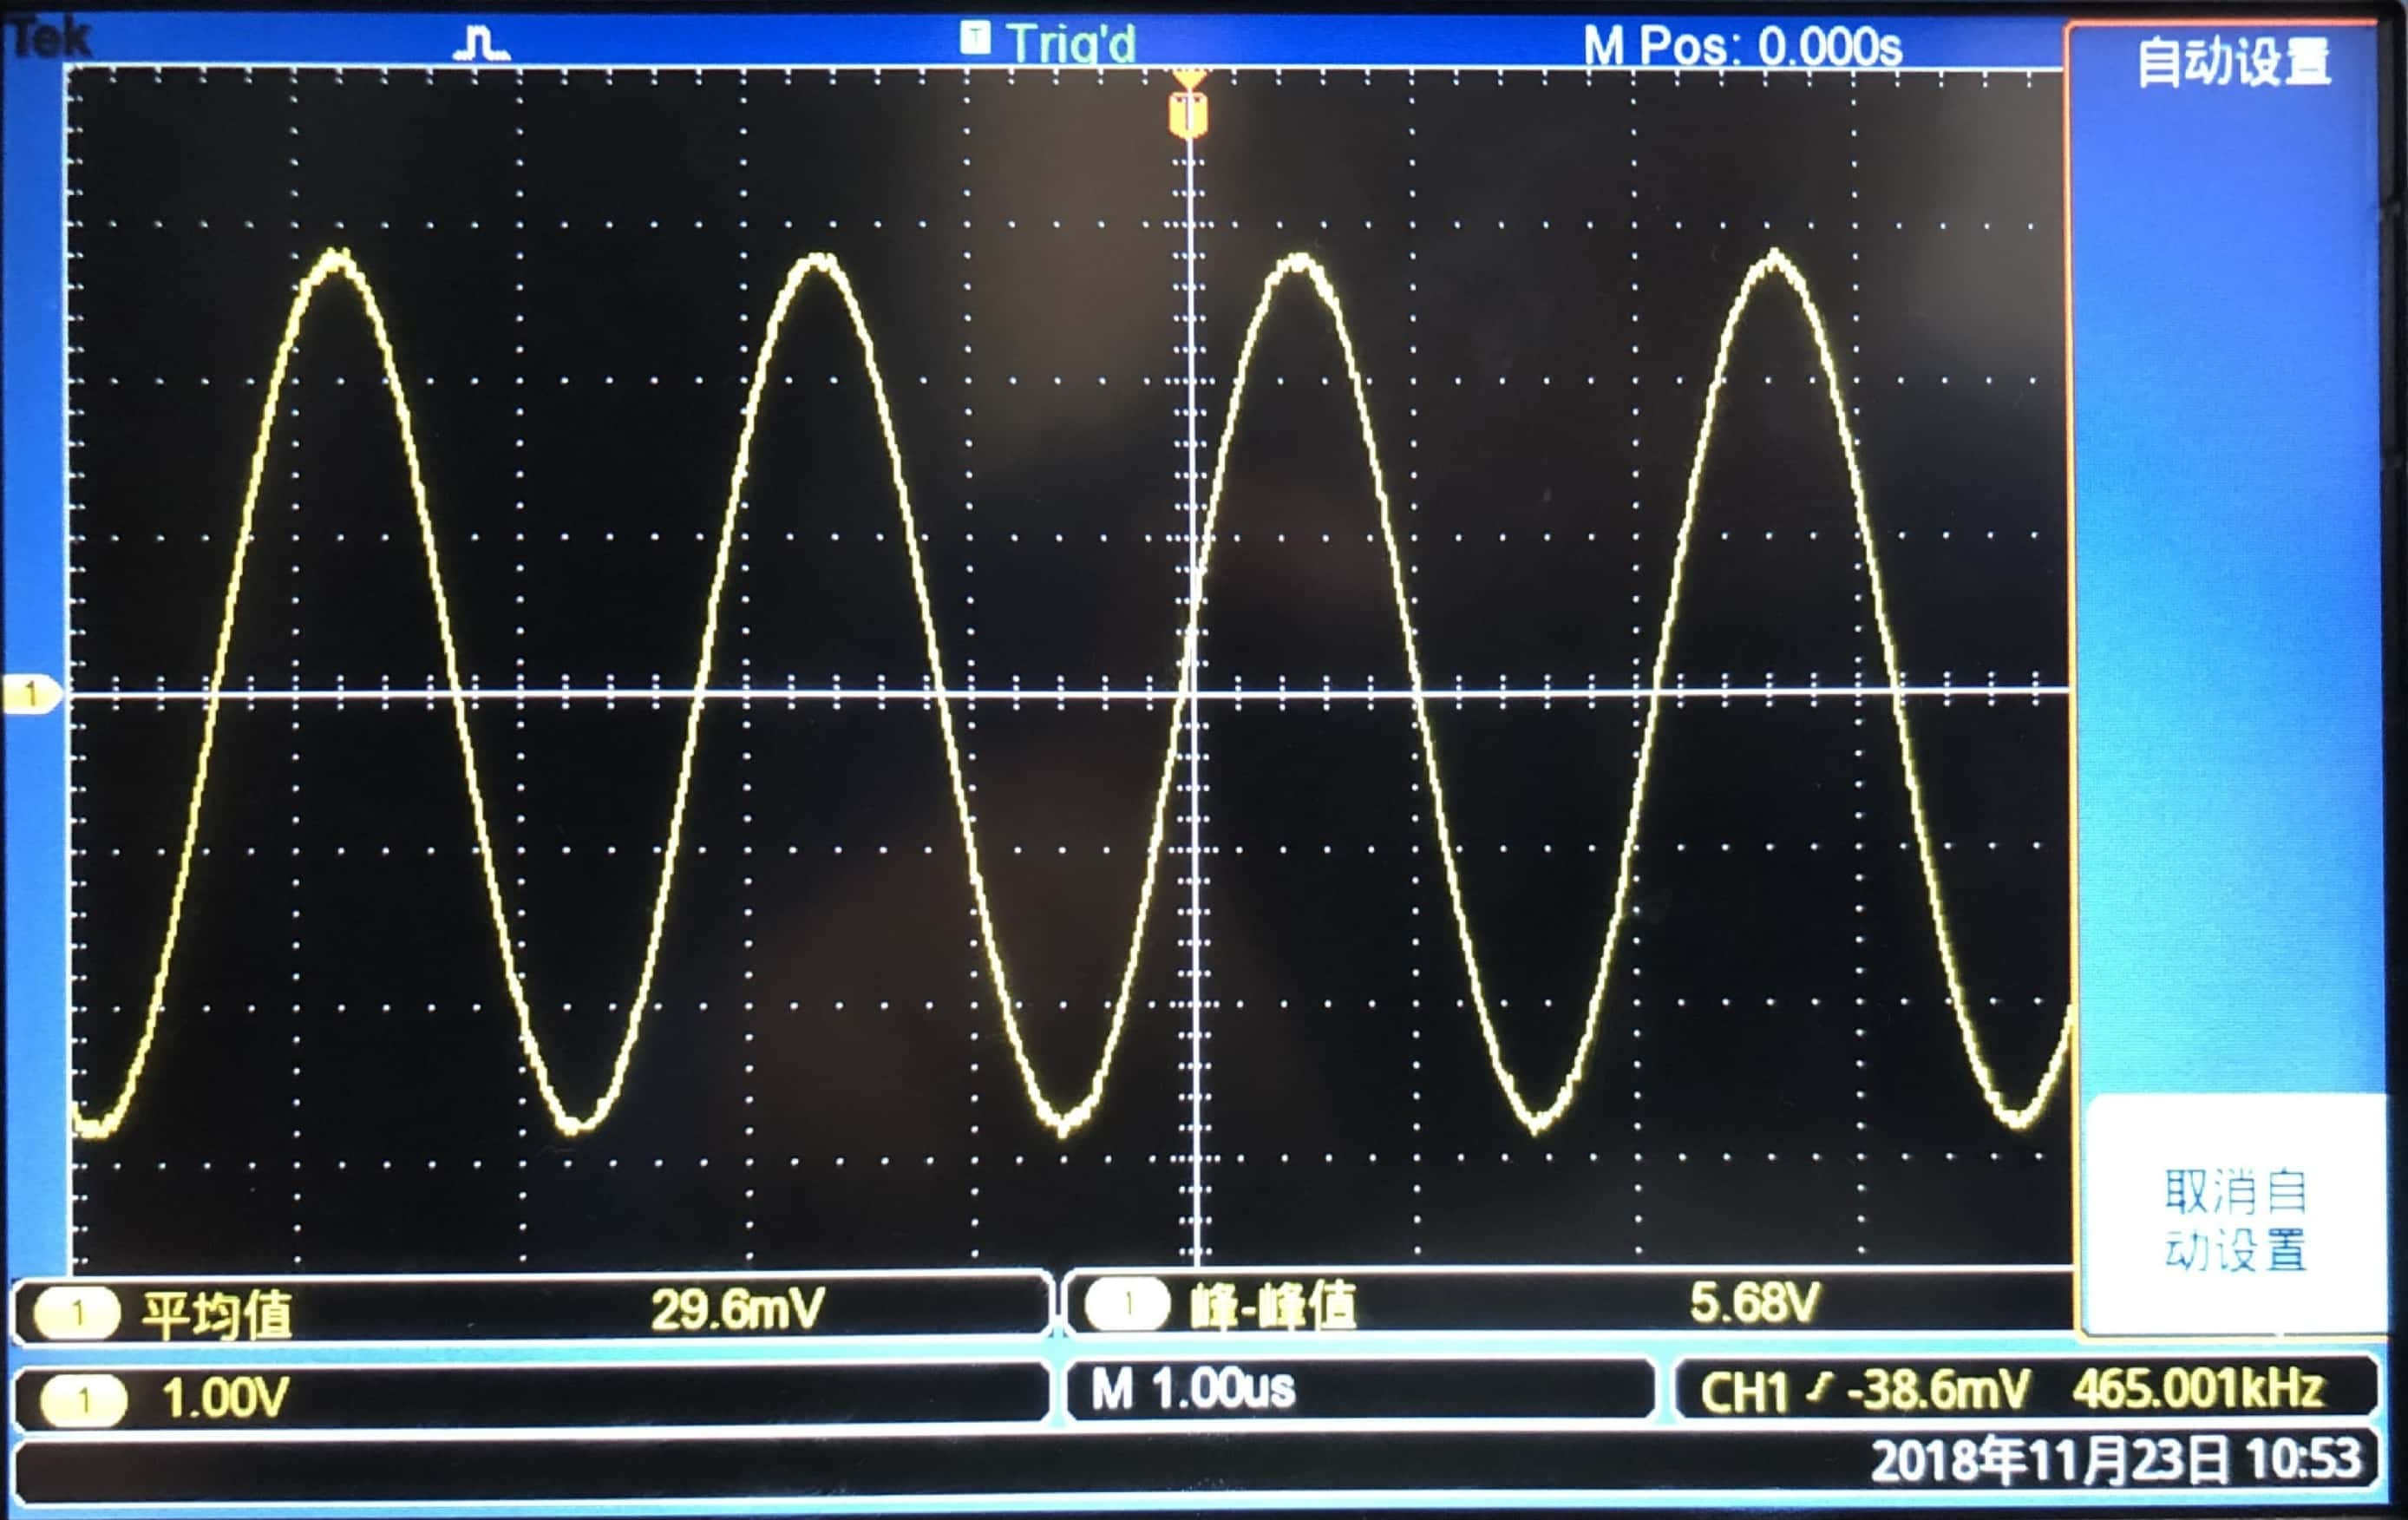
\includegraphics[width=0.35\textwidth]{gaopin2/gaopin216.jpg}      \\ \hline
\end{tabular}
\end{table}
\begin{equation}\label{g:1e}
A_{v0}=\frac{V_{o}}{V_i}=\frac{5.68v}{236mv}=24.07
\end{equation}
其二是在谐振回路的调试时,对双调谐回路的两个中周要反复调试才能最终使谐振回路谐振在输入信号的频点上,具体方法是,连接好测试电路并打开信号源及放大器电源之后,首先调试放大电路的第一级中周,让示波器上被测信号幅度尽可能大,然后调试第二级中周,也是让示波器上被测信号的幅度尽可能大,这之后再重复调第一级和第二级中周,直到输出信号的幅度达到最大,这样,放大器就已经谐振到输入信号的频点上了。\par
同单调谐实验,做双调谐实验,并将两种调谐电路进行比较。(以2KHz为步进间隔来变化)。记录数据如表\ref{tab:bg},在如图\ref{img:cf}的“幅度-频率”坐标轴上标示出放大器的通频带特性。
\begin{table}[htbp]
\centering
\caption{双调谐放大器幅度-频率关系}
\label{tab:bg}
\begin{tabular}{|c|c|}
\hline
输入频率$(KHz)$ & 输出幅度$(V)$ \\ \hline
457         & 0.704     \\ \hline
459         & 1.10      \\ \hline
461         & 2.44      \\ \hline
463         & 4.80      \\ \hline
465         & 5.68      \\ \hline
467         & 5.40      \\ \hline
469         & 4.72      \\ \hline
471         & 4.00      \\ \hline
473         & 3.40      \\ \hline
\end{tabular}
\end{table}

\subsection{实验仪器}
\begin{tabular}{clcc}
1.&高频实验箱&&         1台 \\2.&双踪示波器& &    1台\\3.&  万用表&&             1块\\ 4.&扫频仪(可选)&&       1台\\
\end{tabular}
\subsection{实验结果}
\begin{enumerate}\addtolength{\itemsep}{-1.5ex}
\item 由图\ref{img:c}可知,对于本实验的单调谐放大器而言,有:$$f_L=11.427MHz $$ $$f_H=12.561MHz $$$$B=1.134MHz$$\par
  \begin{figure}[ht]
  \centering
  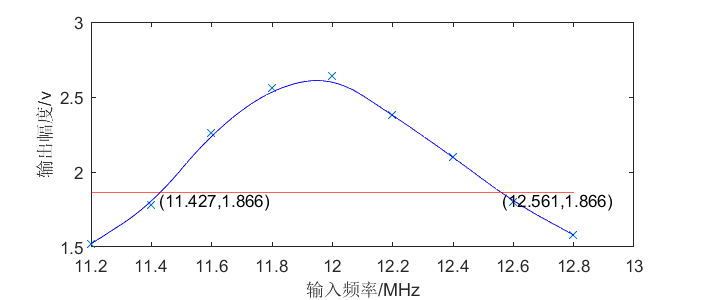
\includegraphics[width=\textwidth]{gaopin2/untitled1.png} 
  \caption{ 单调谐放大器幅度-频率关系拟合图} 
  \label{img:c} 
\end{figure}
\item 同样,由图\ref{img:cf}可知,对于本实验的双调谐放大器而言,有:$$f_L=462.48KHz $$ $$f_H=470.70KHz $$$$B=8.22KHz$$\par
  \begin{figure}[ht]
  \centering
  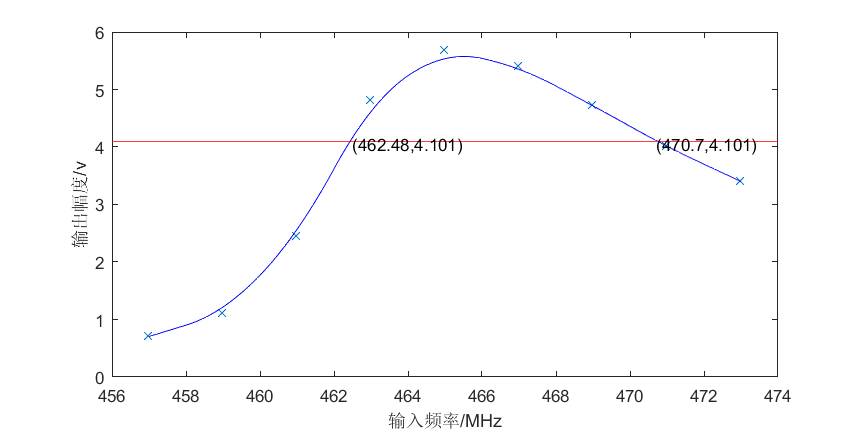
\includegraphics[width=\textwidth]{gaopin2/untitled2.png} 
  \caption{ 双调谐放大器幅度-频率关系拟合图} 
  \label{img:cf} 
\end{figure}
\item  单调谐小信号放大器输出信号波形见图\ref{img:121};
\item 双调谐小信号放大器输出信号波形见图\ref{img:122}。
\begin{figure}[htbp]
\centering
\begin{tabular}{ccc}
 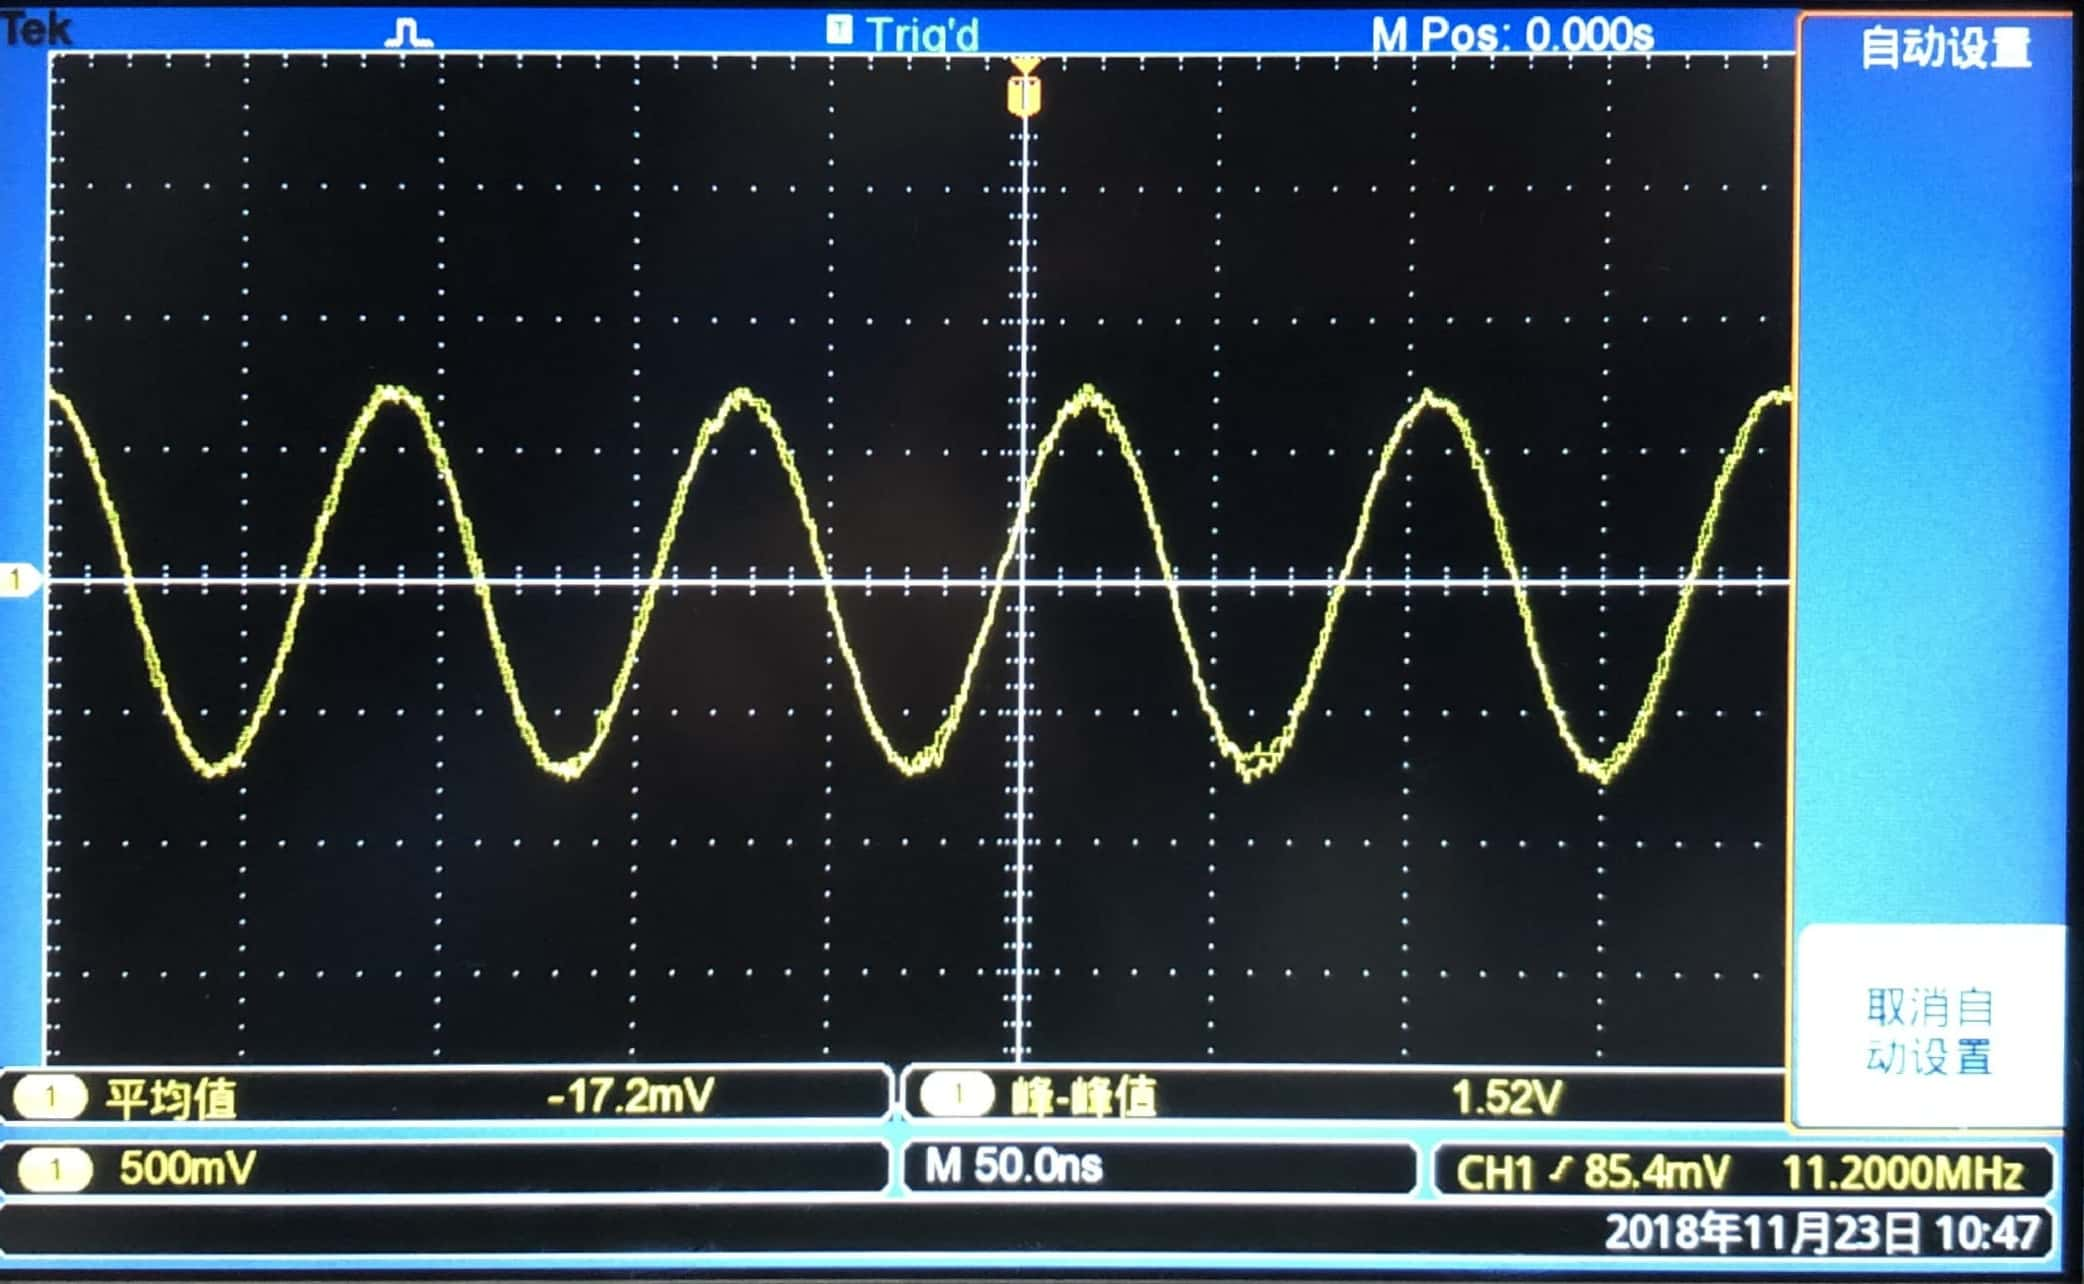
\includegraphics[width=0.35\textwidth]{gaopin2/gaopin213.jpg} &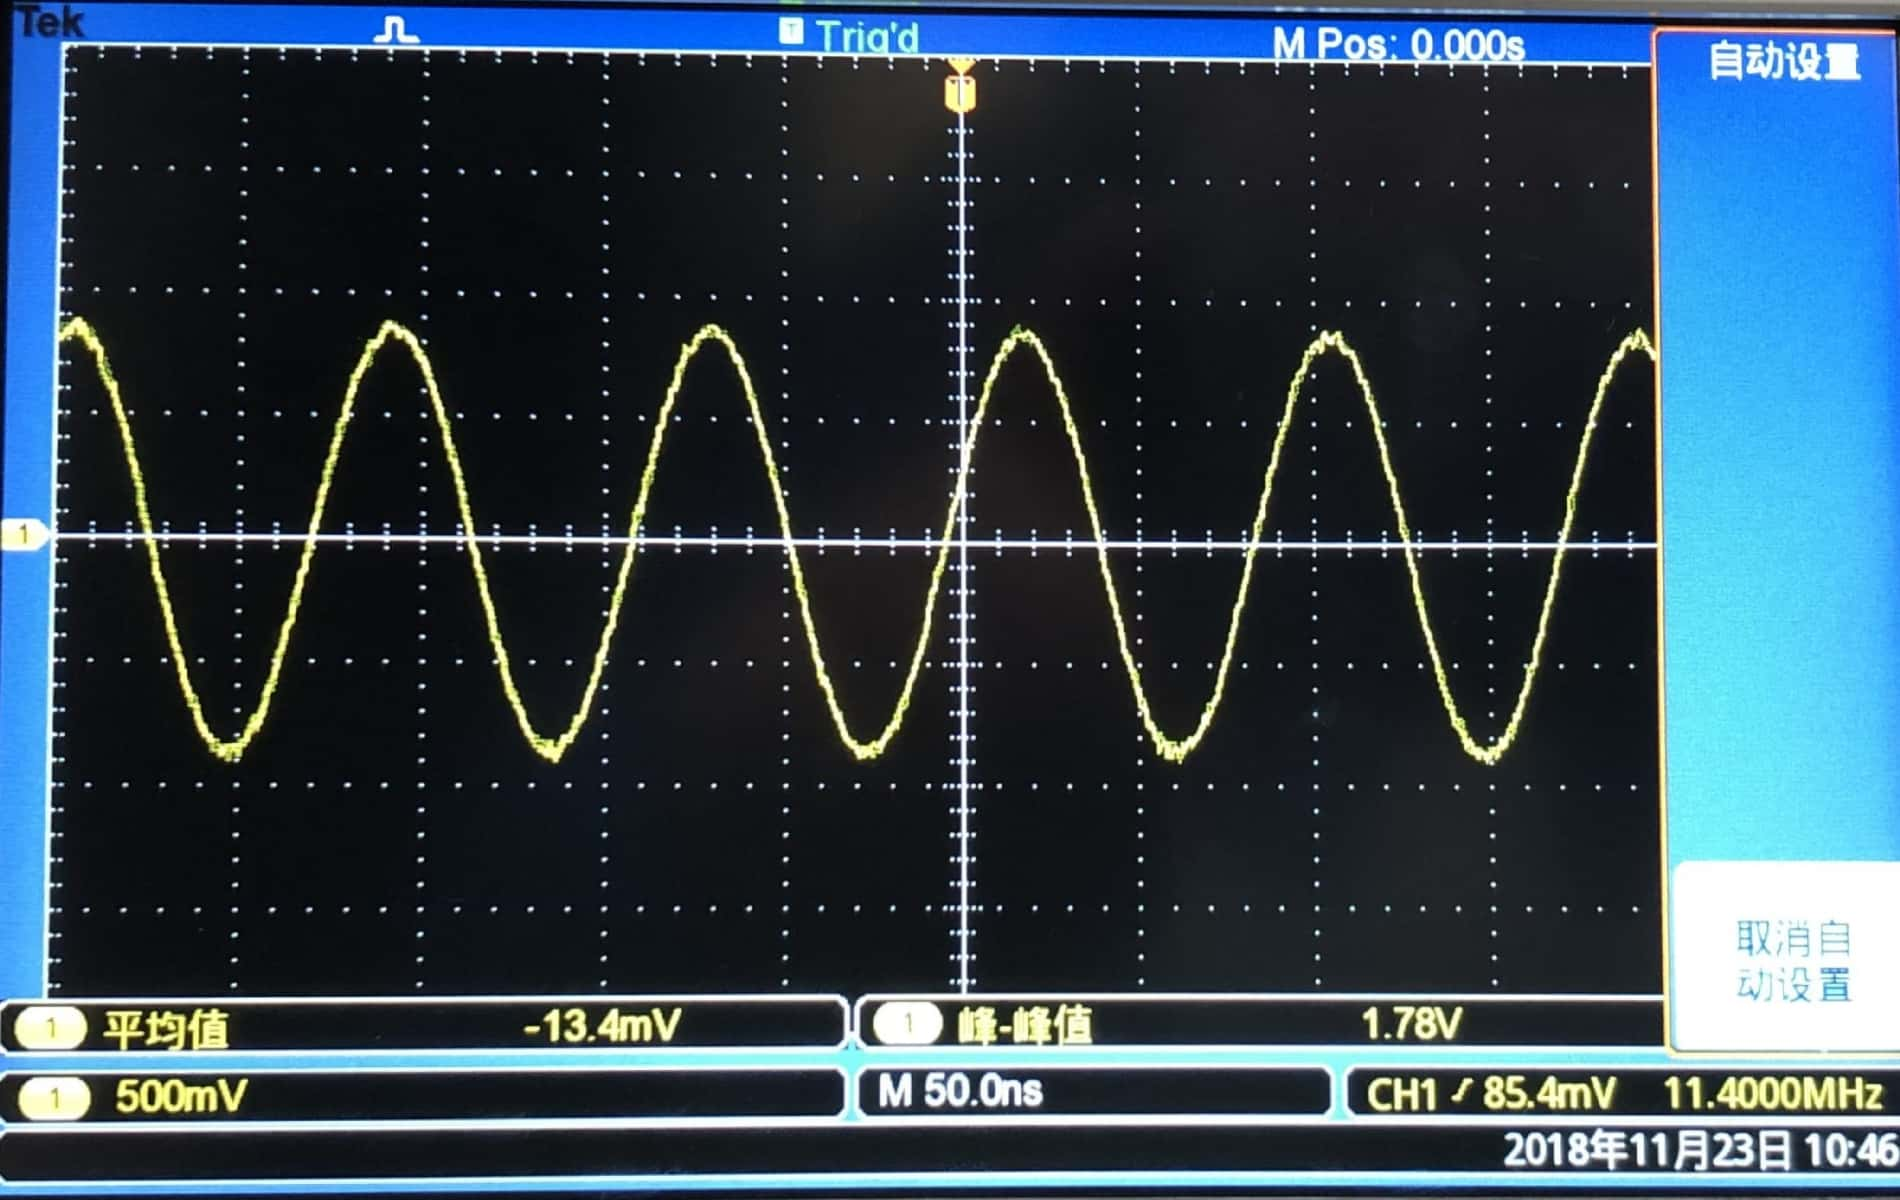
\includegraphics[width=0.35\textwidth]{gaopin2/gaopin223.jpg}&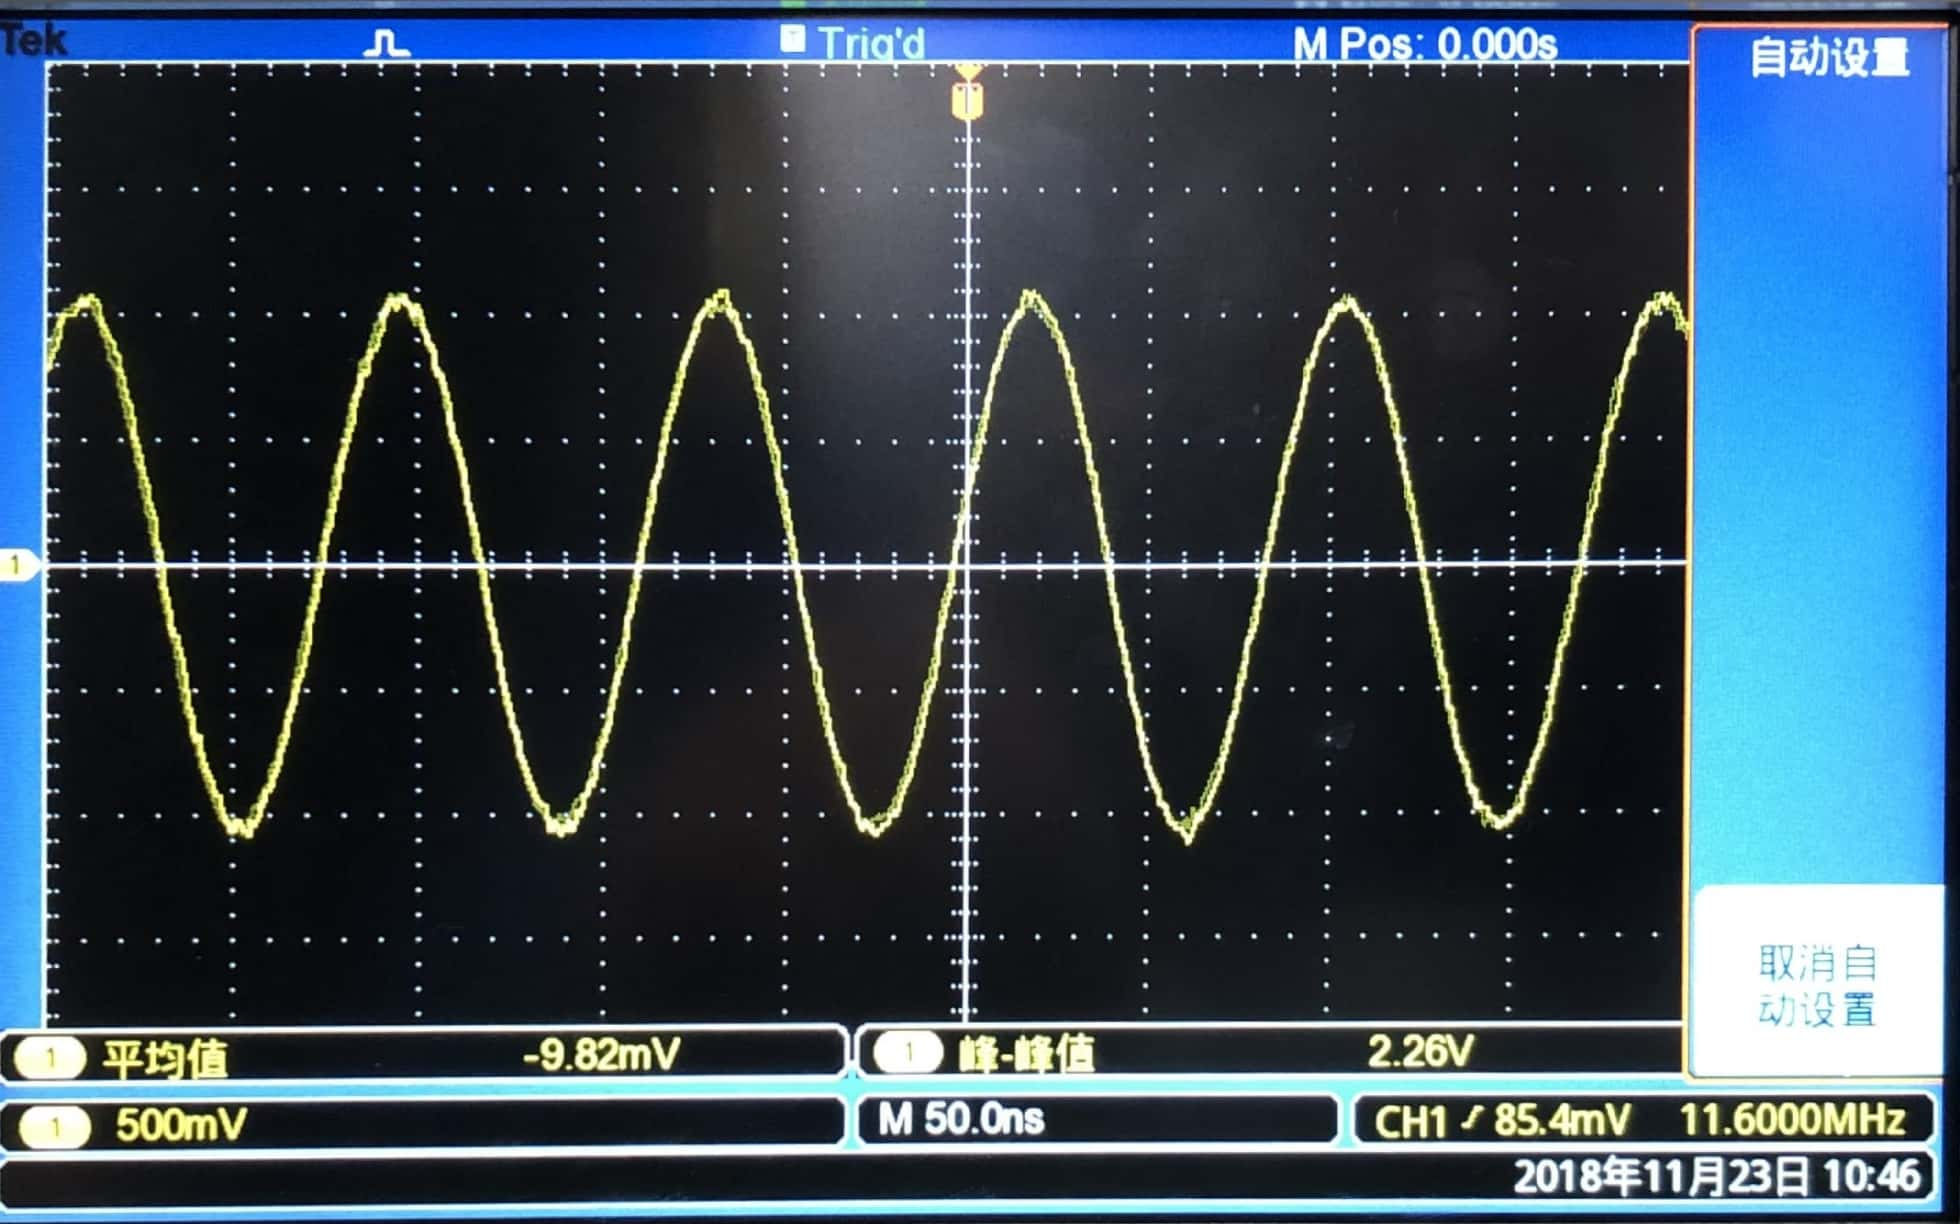
\includegraphics[width=0.35\textwidth]{gaopin2/gaopin212.jpg} \\ 
$f=11.2\ MHz$ & $f=11.4\ MHz$ & $f=11.6\ MHz$ \\
$V_o=1.52\ v$ & $V_o=1.78\ v$ & $V_o=2.26\ v$ \\
\\
 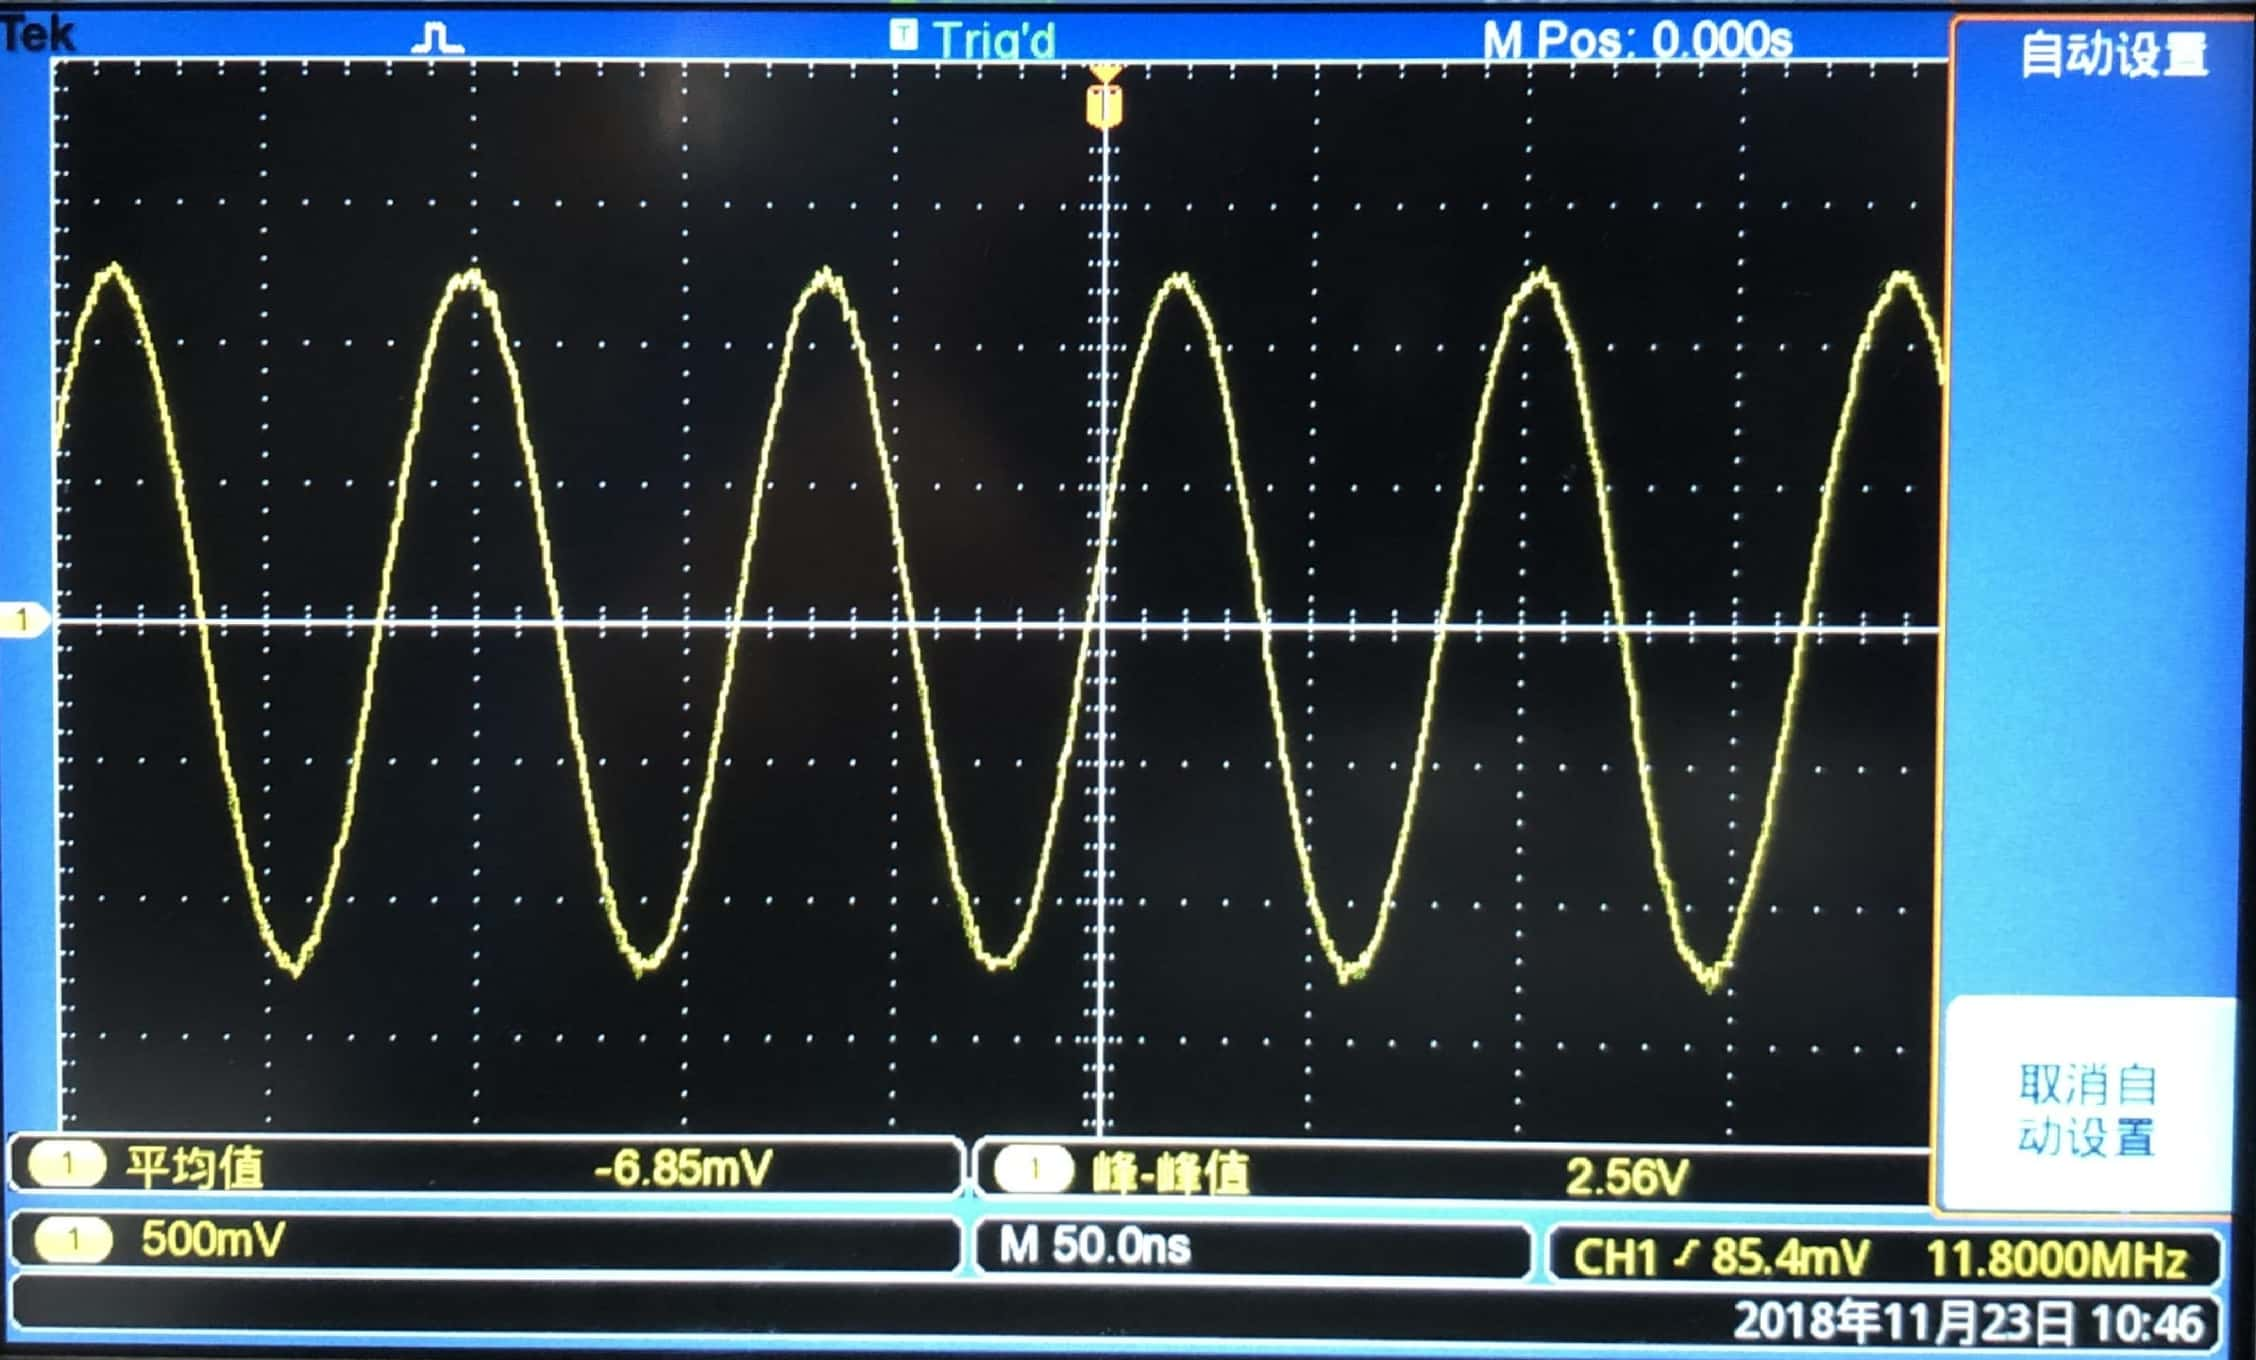
\includegraphics[width=0.35\textwidth]{gaopin2/gaopin206.jpg} &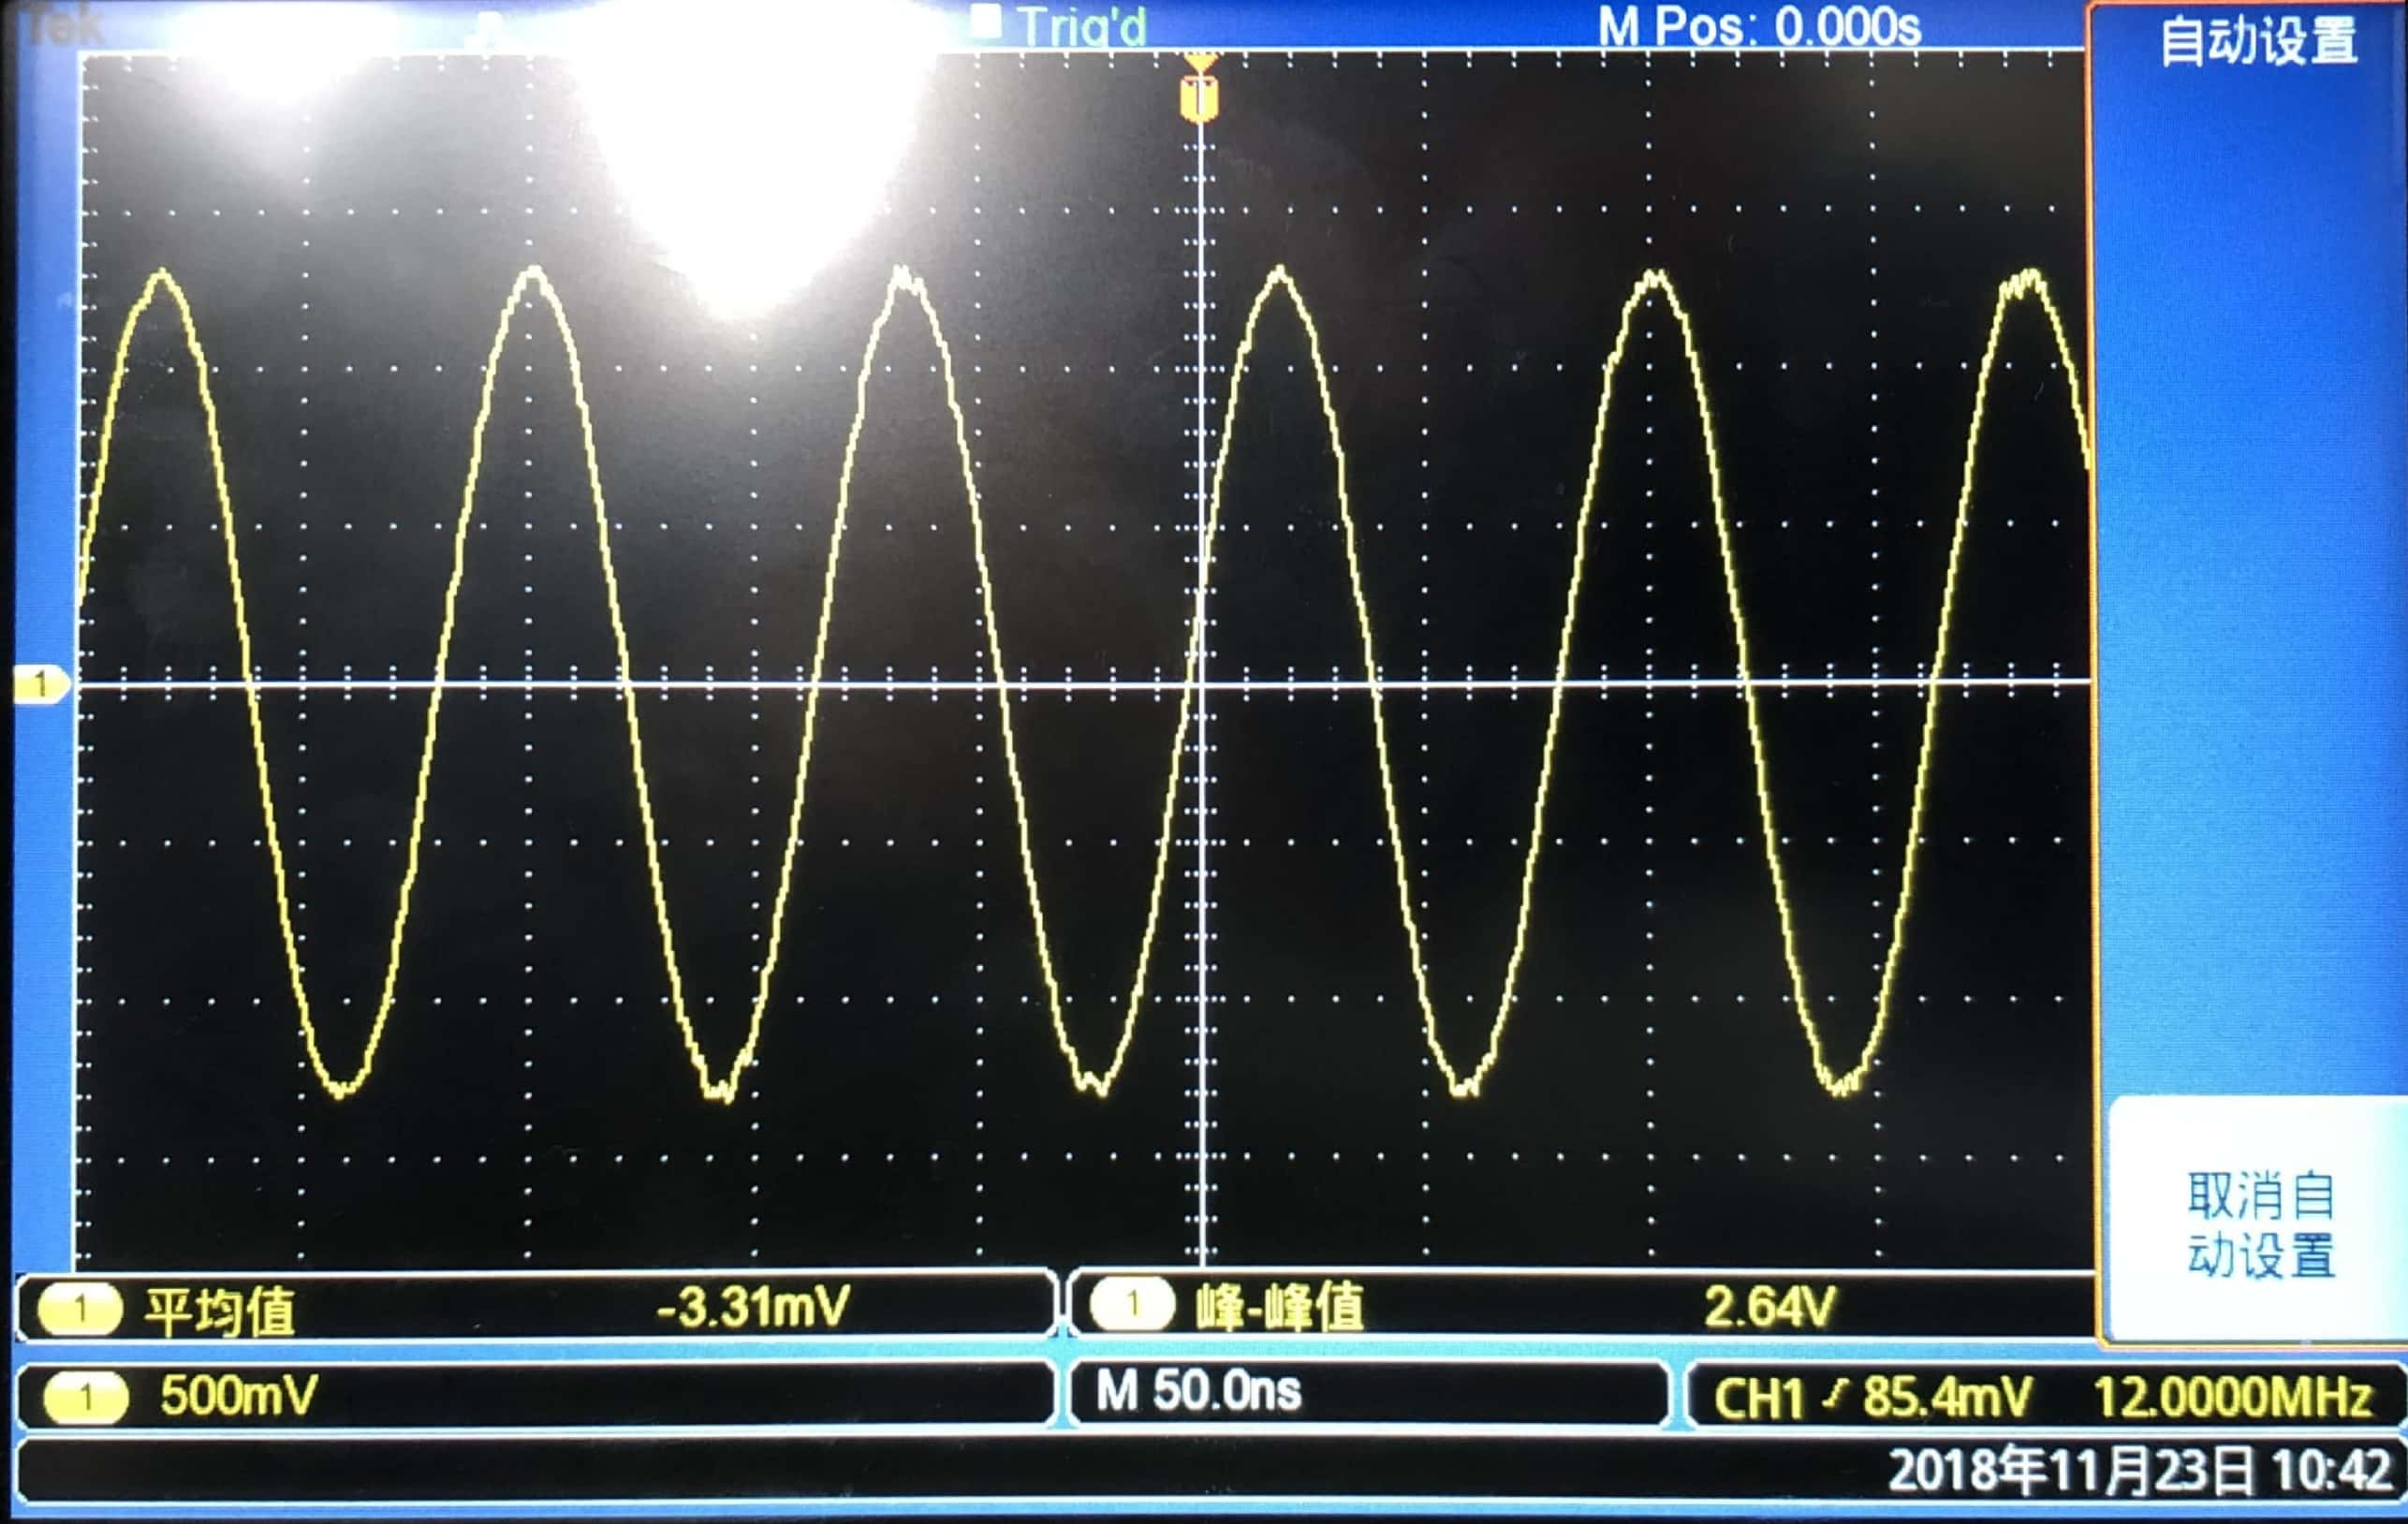
\includegraphics[width=0.35\textwidth]{gaopin2/gaopin208.jpg}&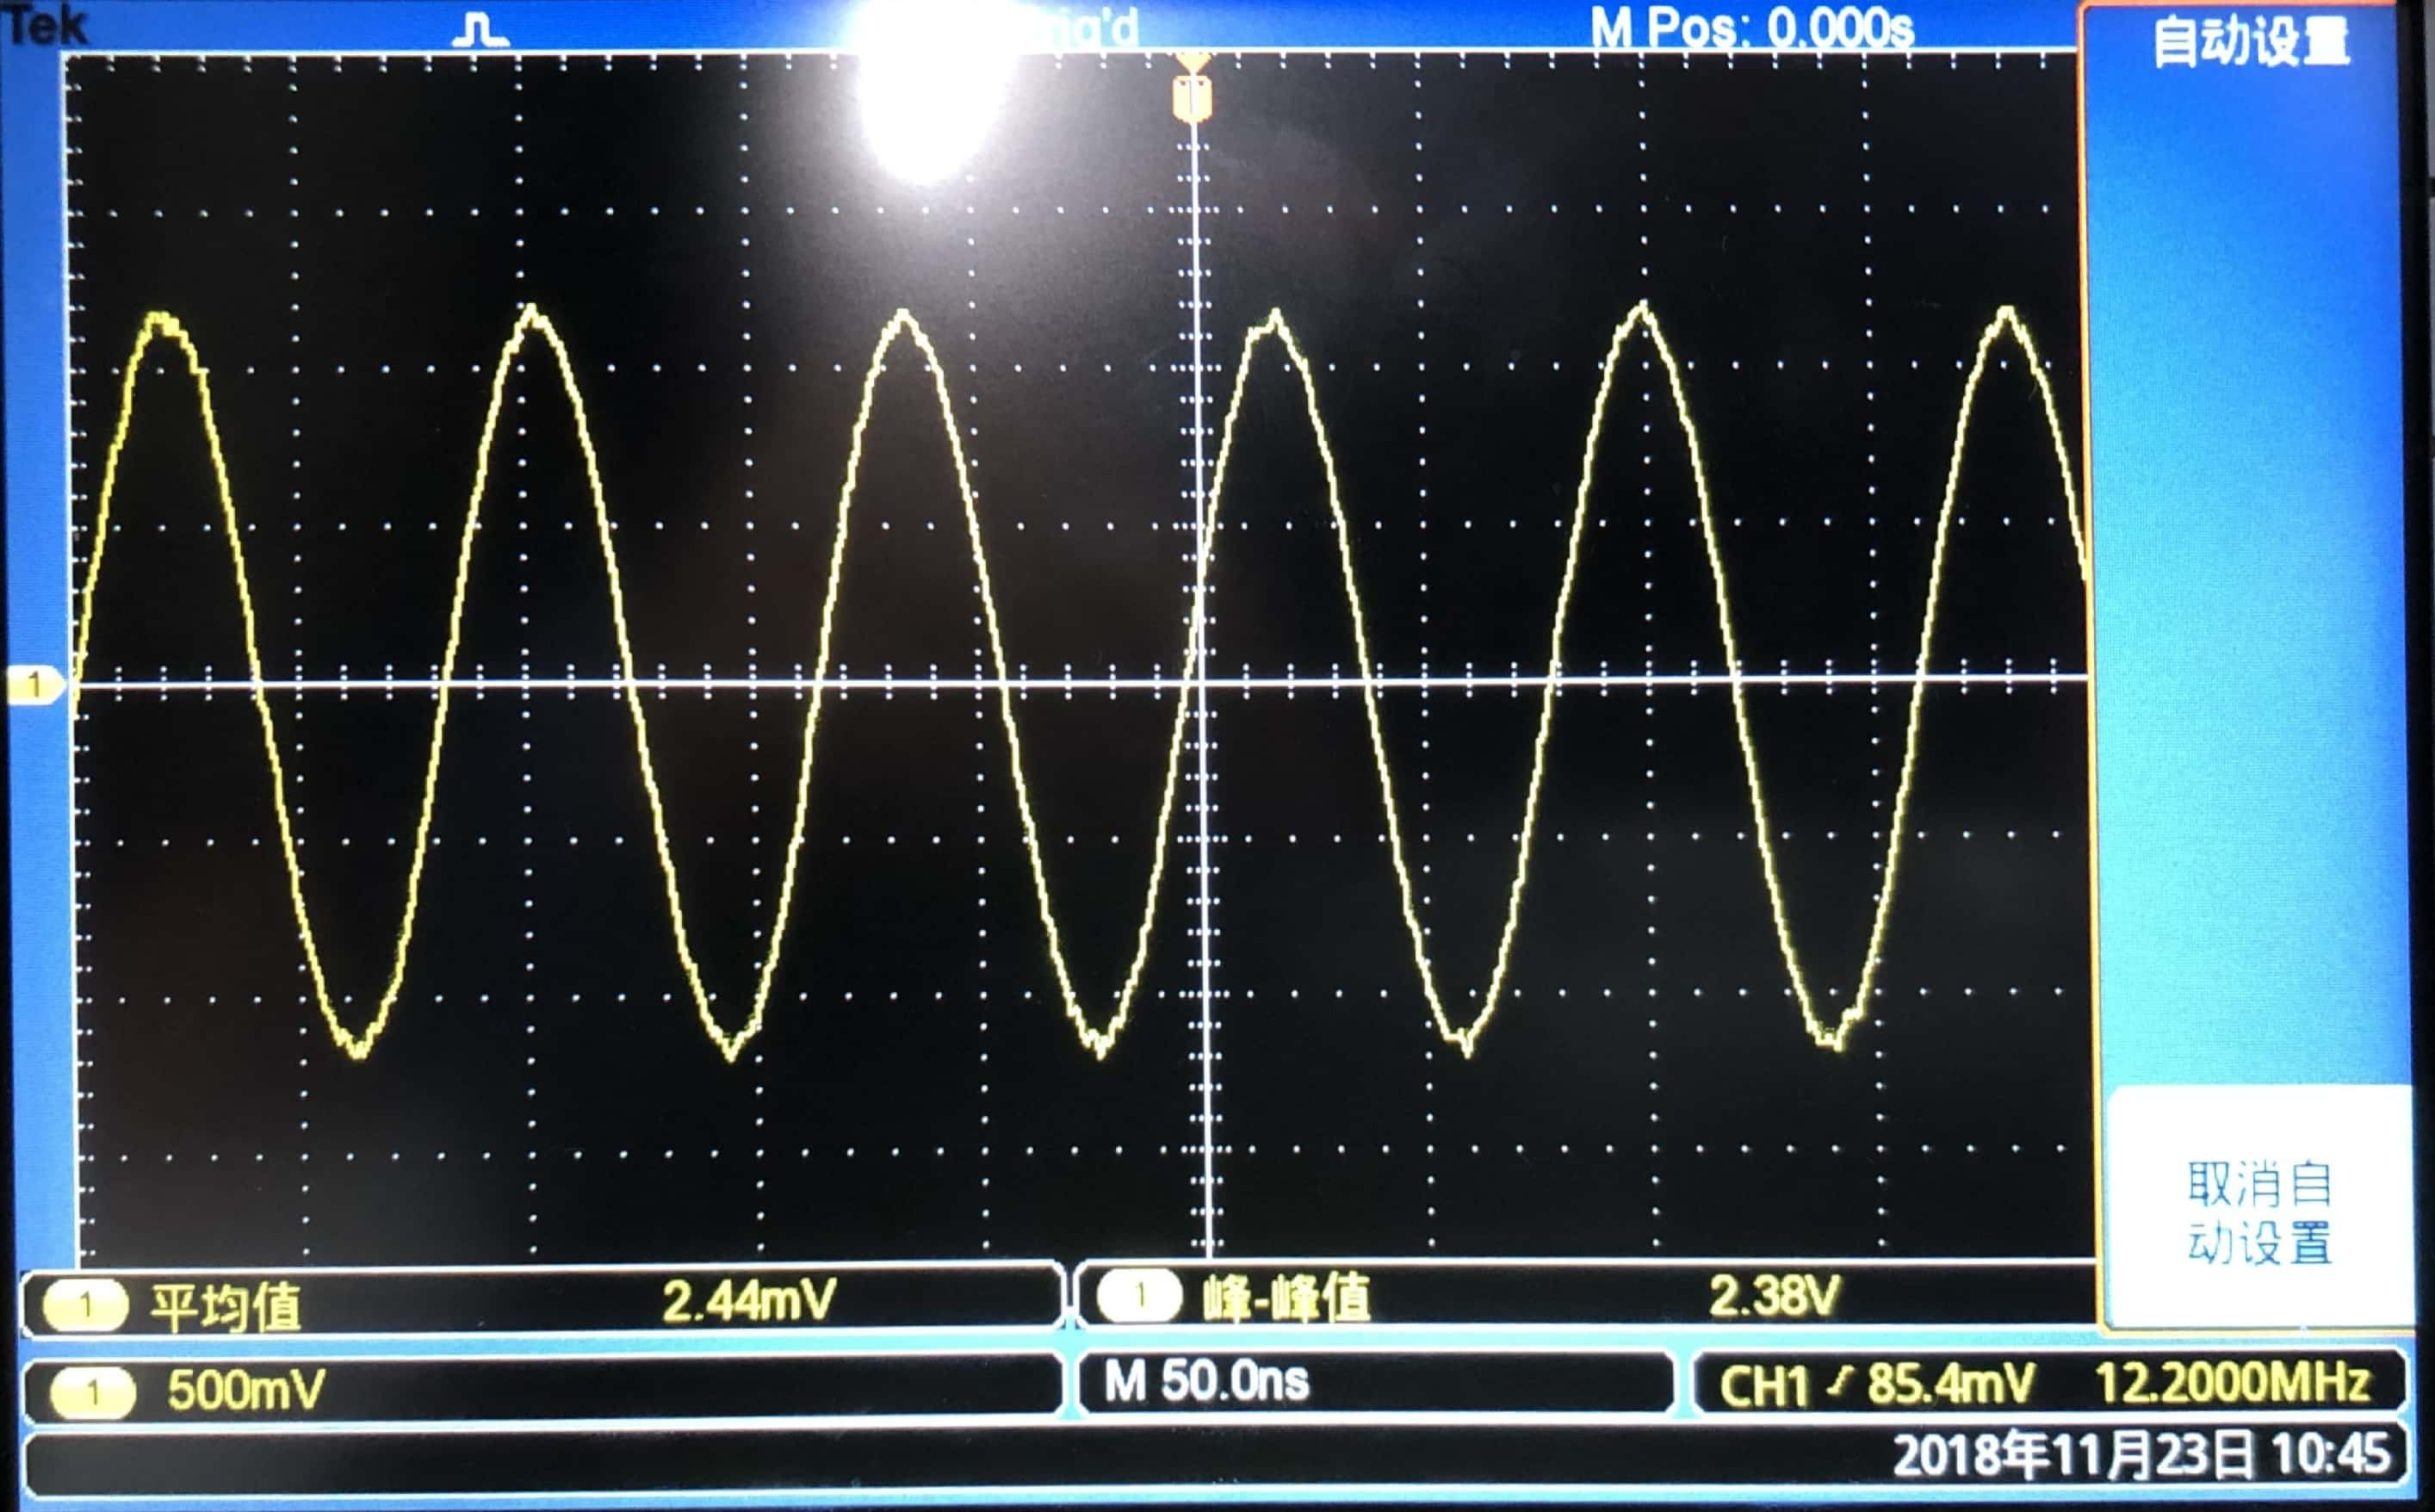
\includegraphics[width=0.35\textwidth]{gaopin2/gaopin220.jpg} \\ 
$f=11.8\ MHz$ & $f=12\ MHz$ & $f=12.2\ MHz$ \\
$V_o=2.56\ v$ & $V_o=2.64\ v$ & $V_o=2.38\ v$ \\
\\
 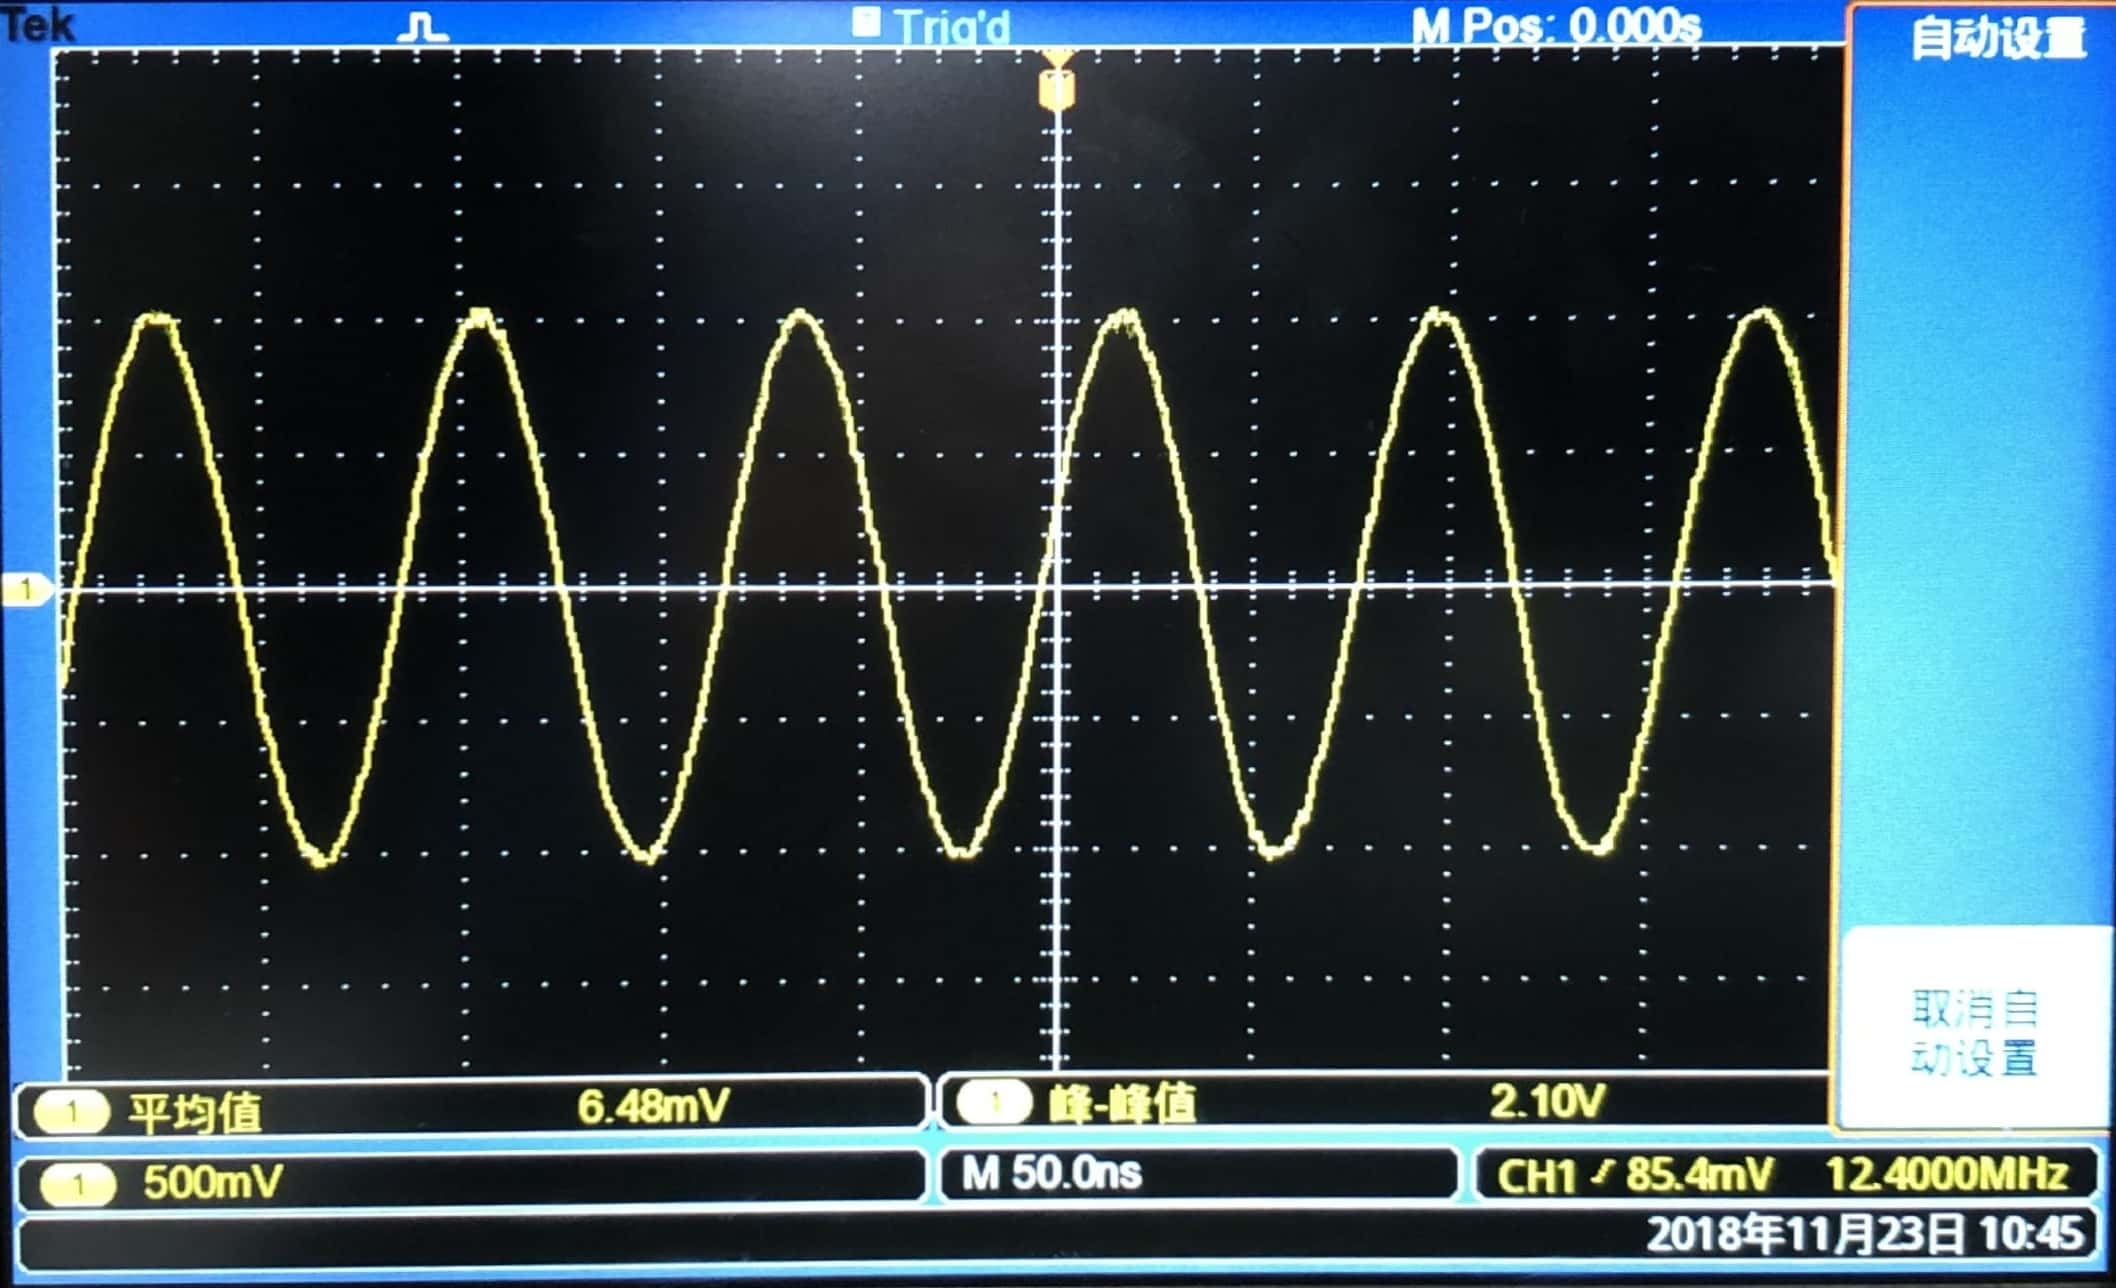
\includegraphics[width=0.35\textwidth]{gaopin2/gaopin214.jpg} &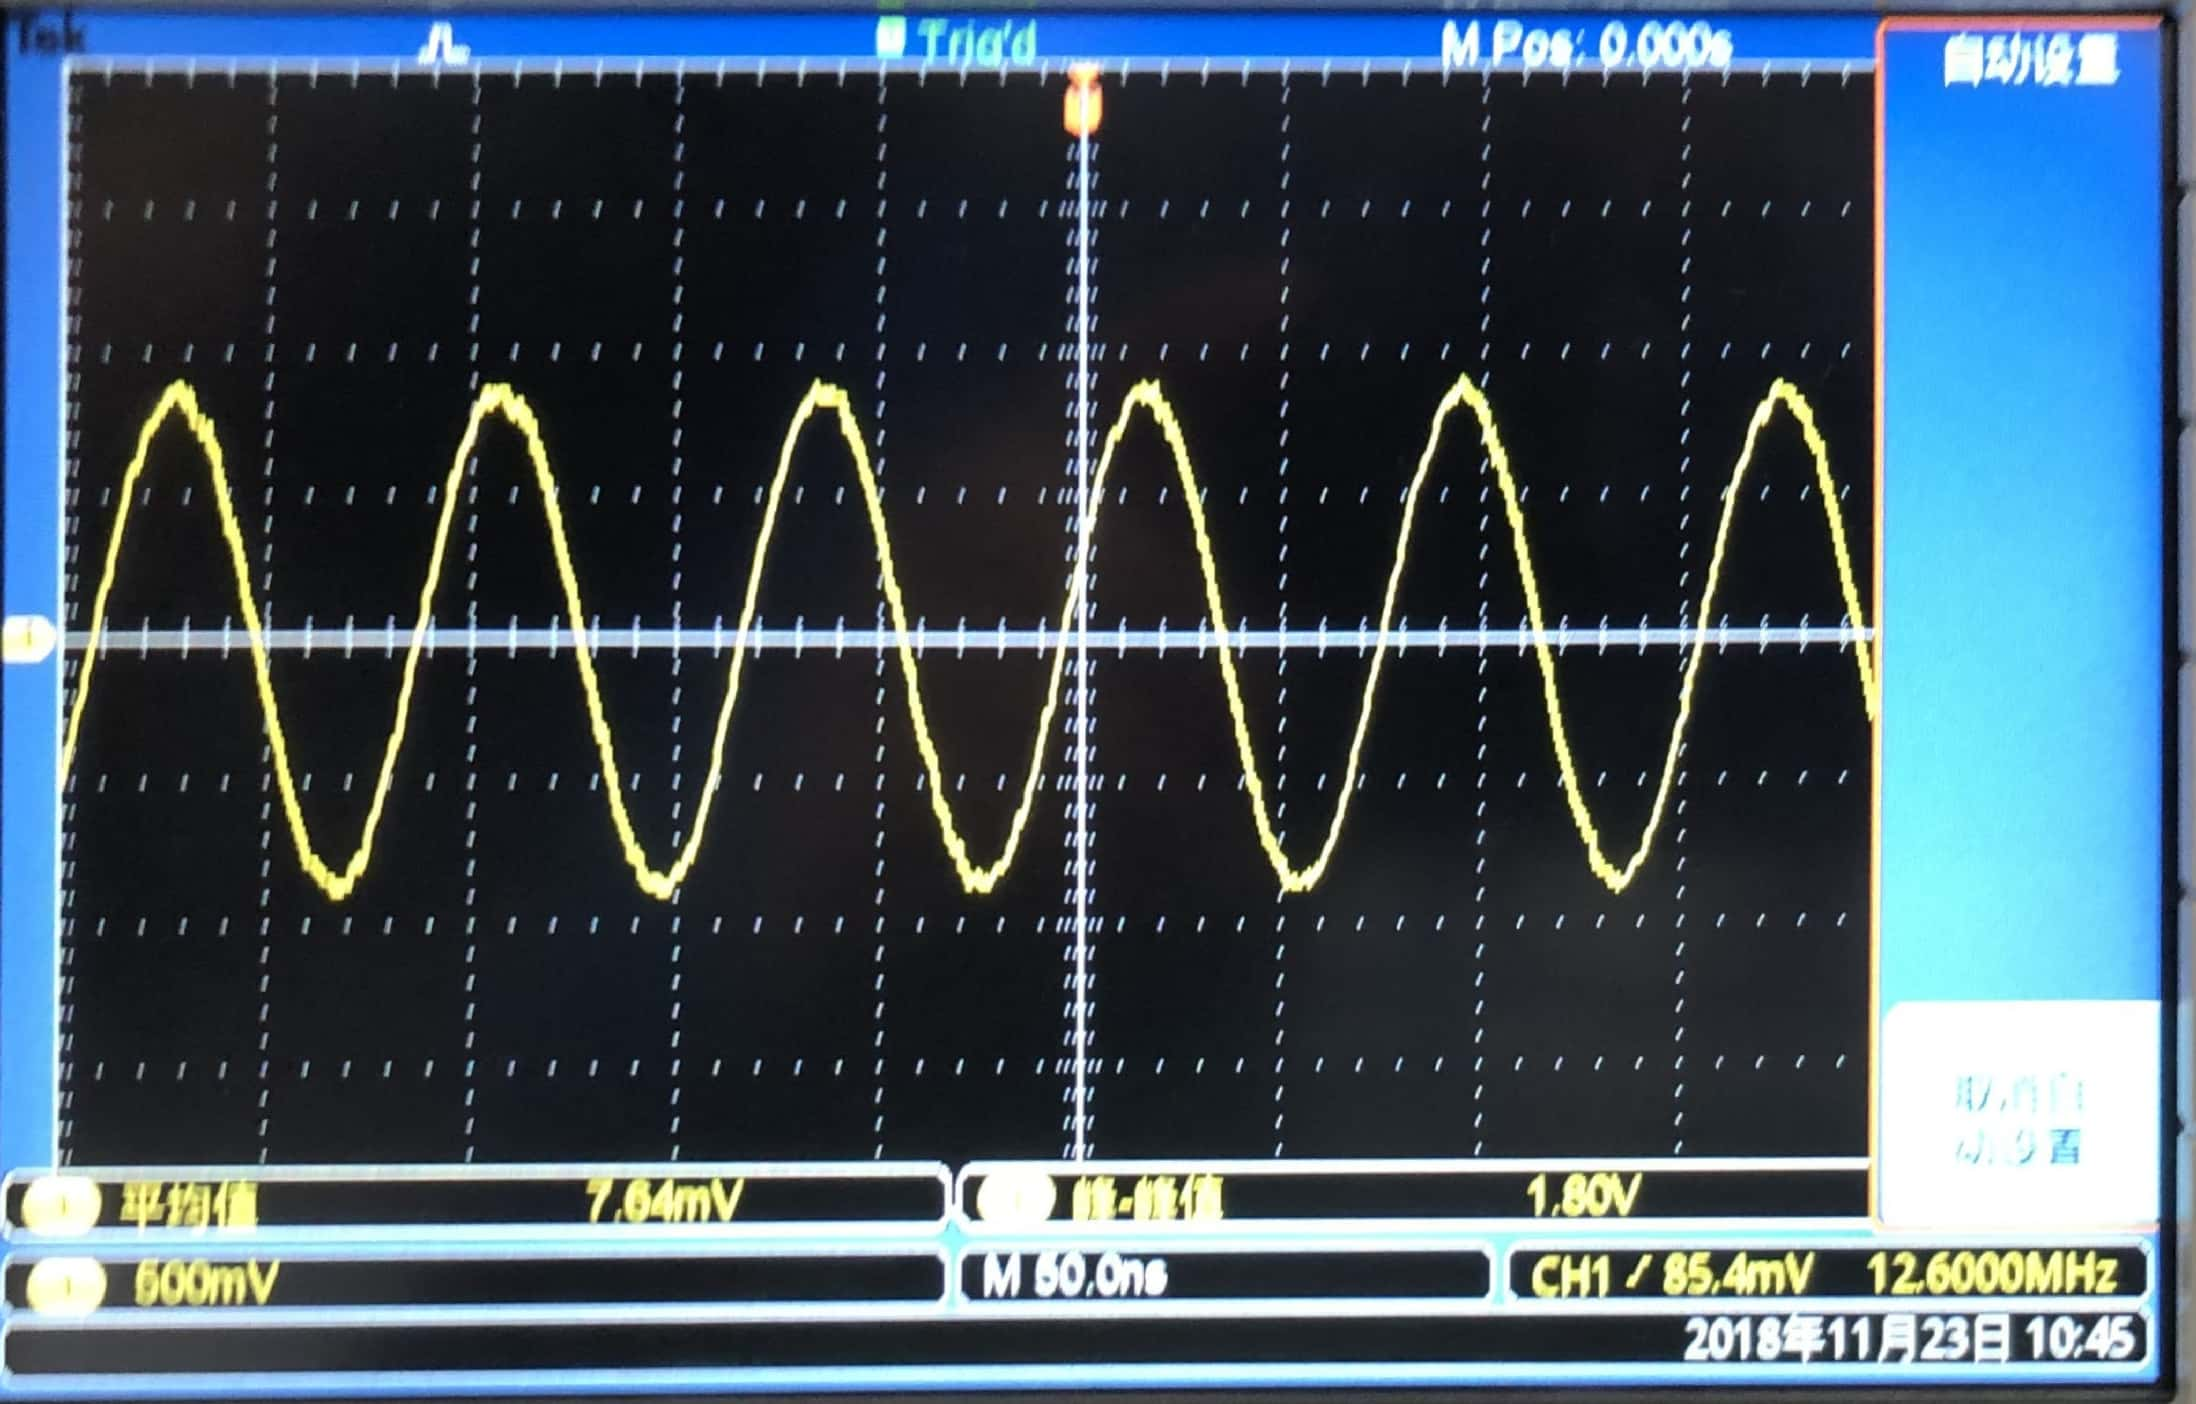
\includegraphics[width=0.35\textwidth]{gaopin2/gaopin217.jpg}&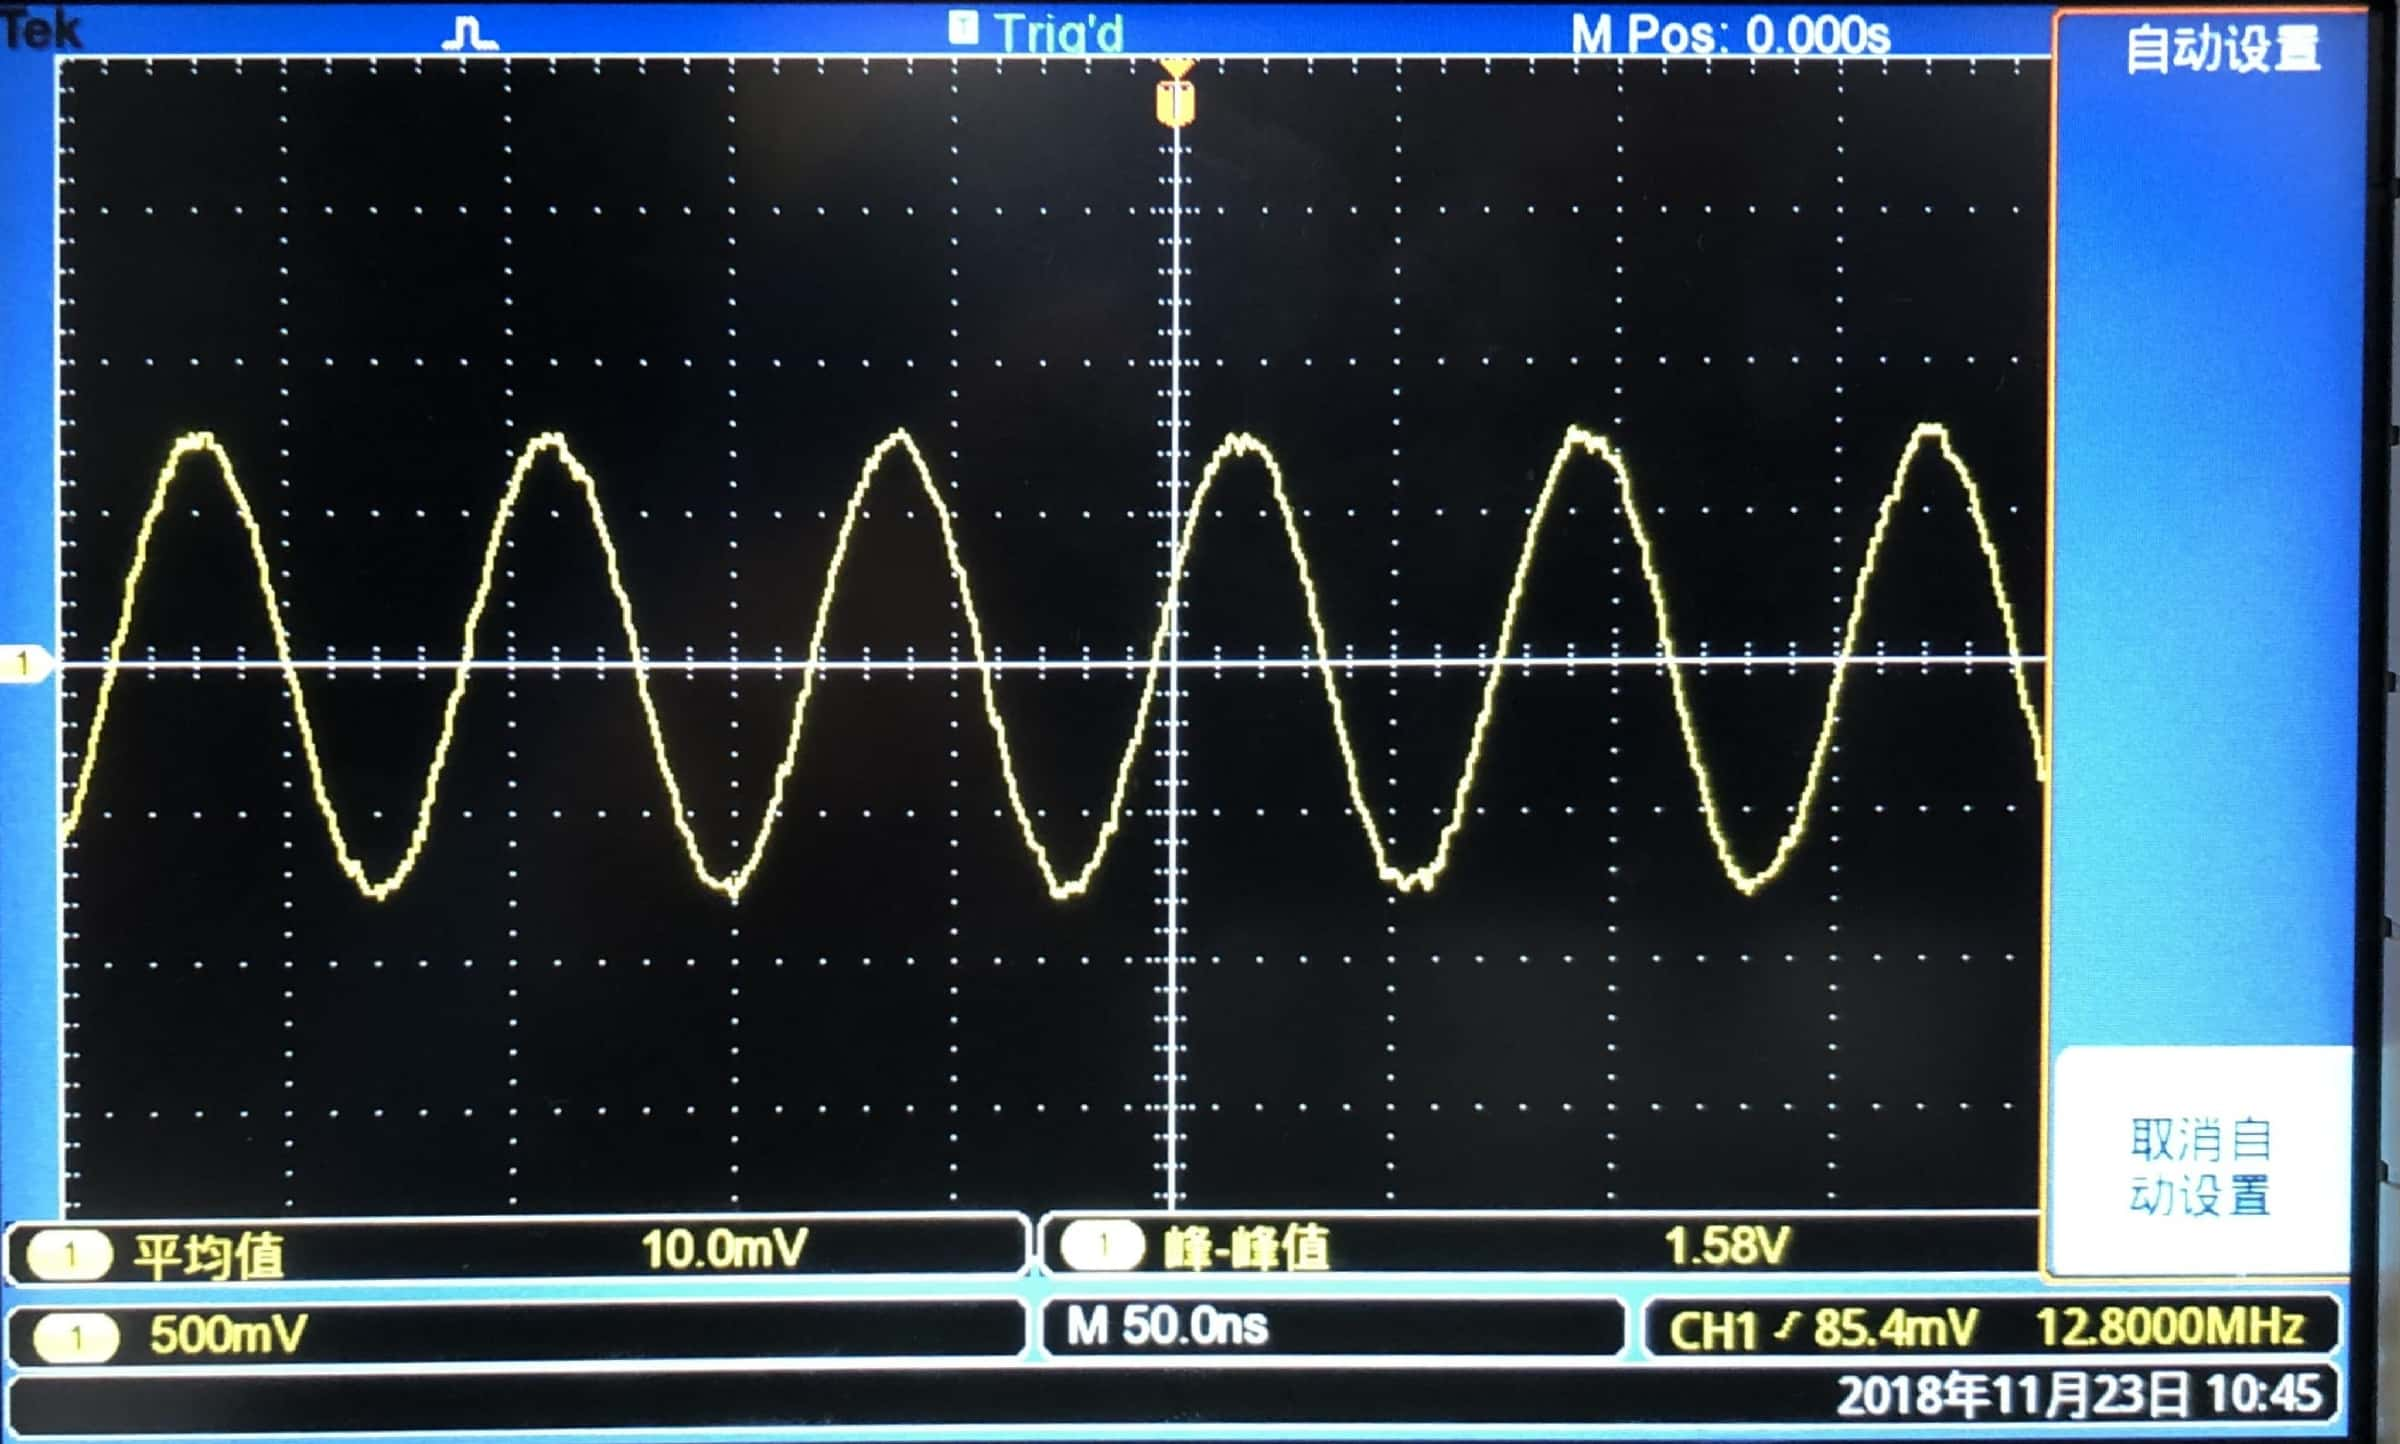
\includegraphics[width=0.35\textwidth]{gaopin2/gaopin219.jpg} \\ 
$f=12.4\ MHz$ & $f=12.6\ MHz$ & $f=12.8\ MHz$ \\
$V_o=2.10\ v$ & $V_o=1.80\ v$ & $V_o=1.58\ v$ \\
\end{tabular}
\caption{单调谐小信号放大器输出信号波形图}\label{img:121}
\end{figure}
\begin{figure}[htbp]
\centering
\begin{tabular}{ccc}
 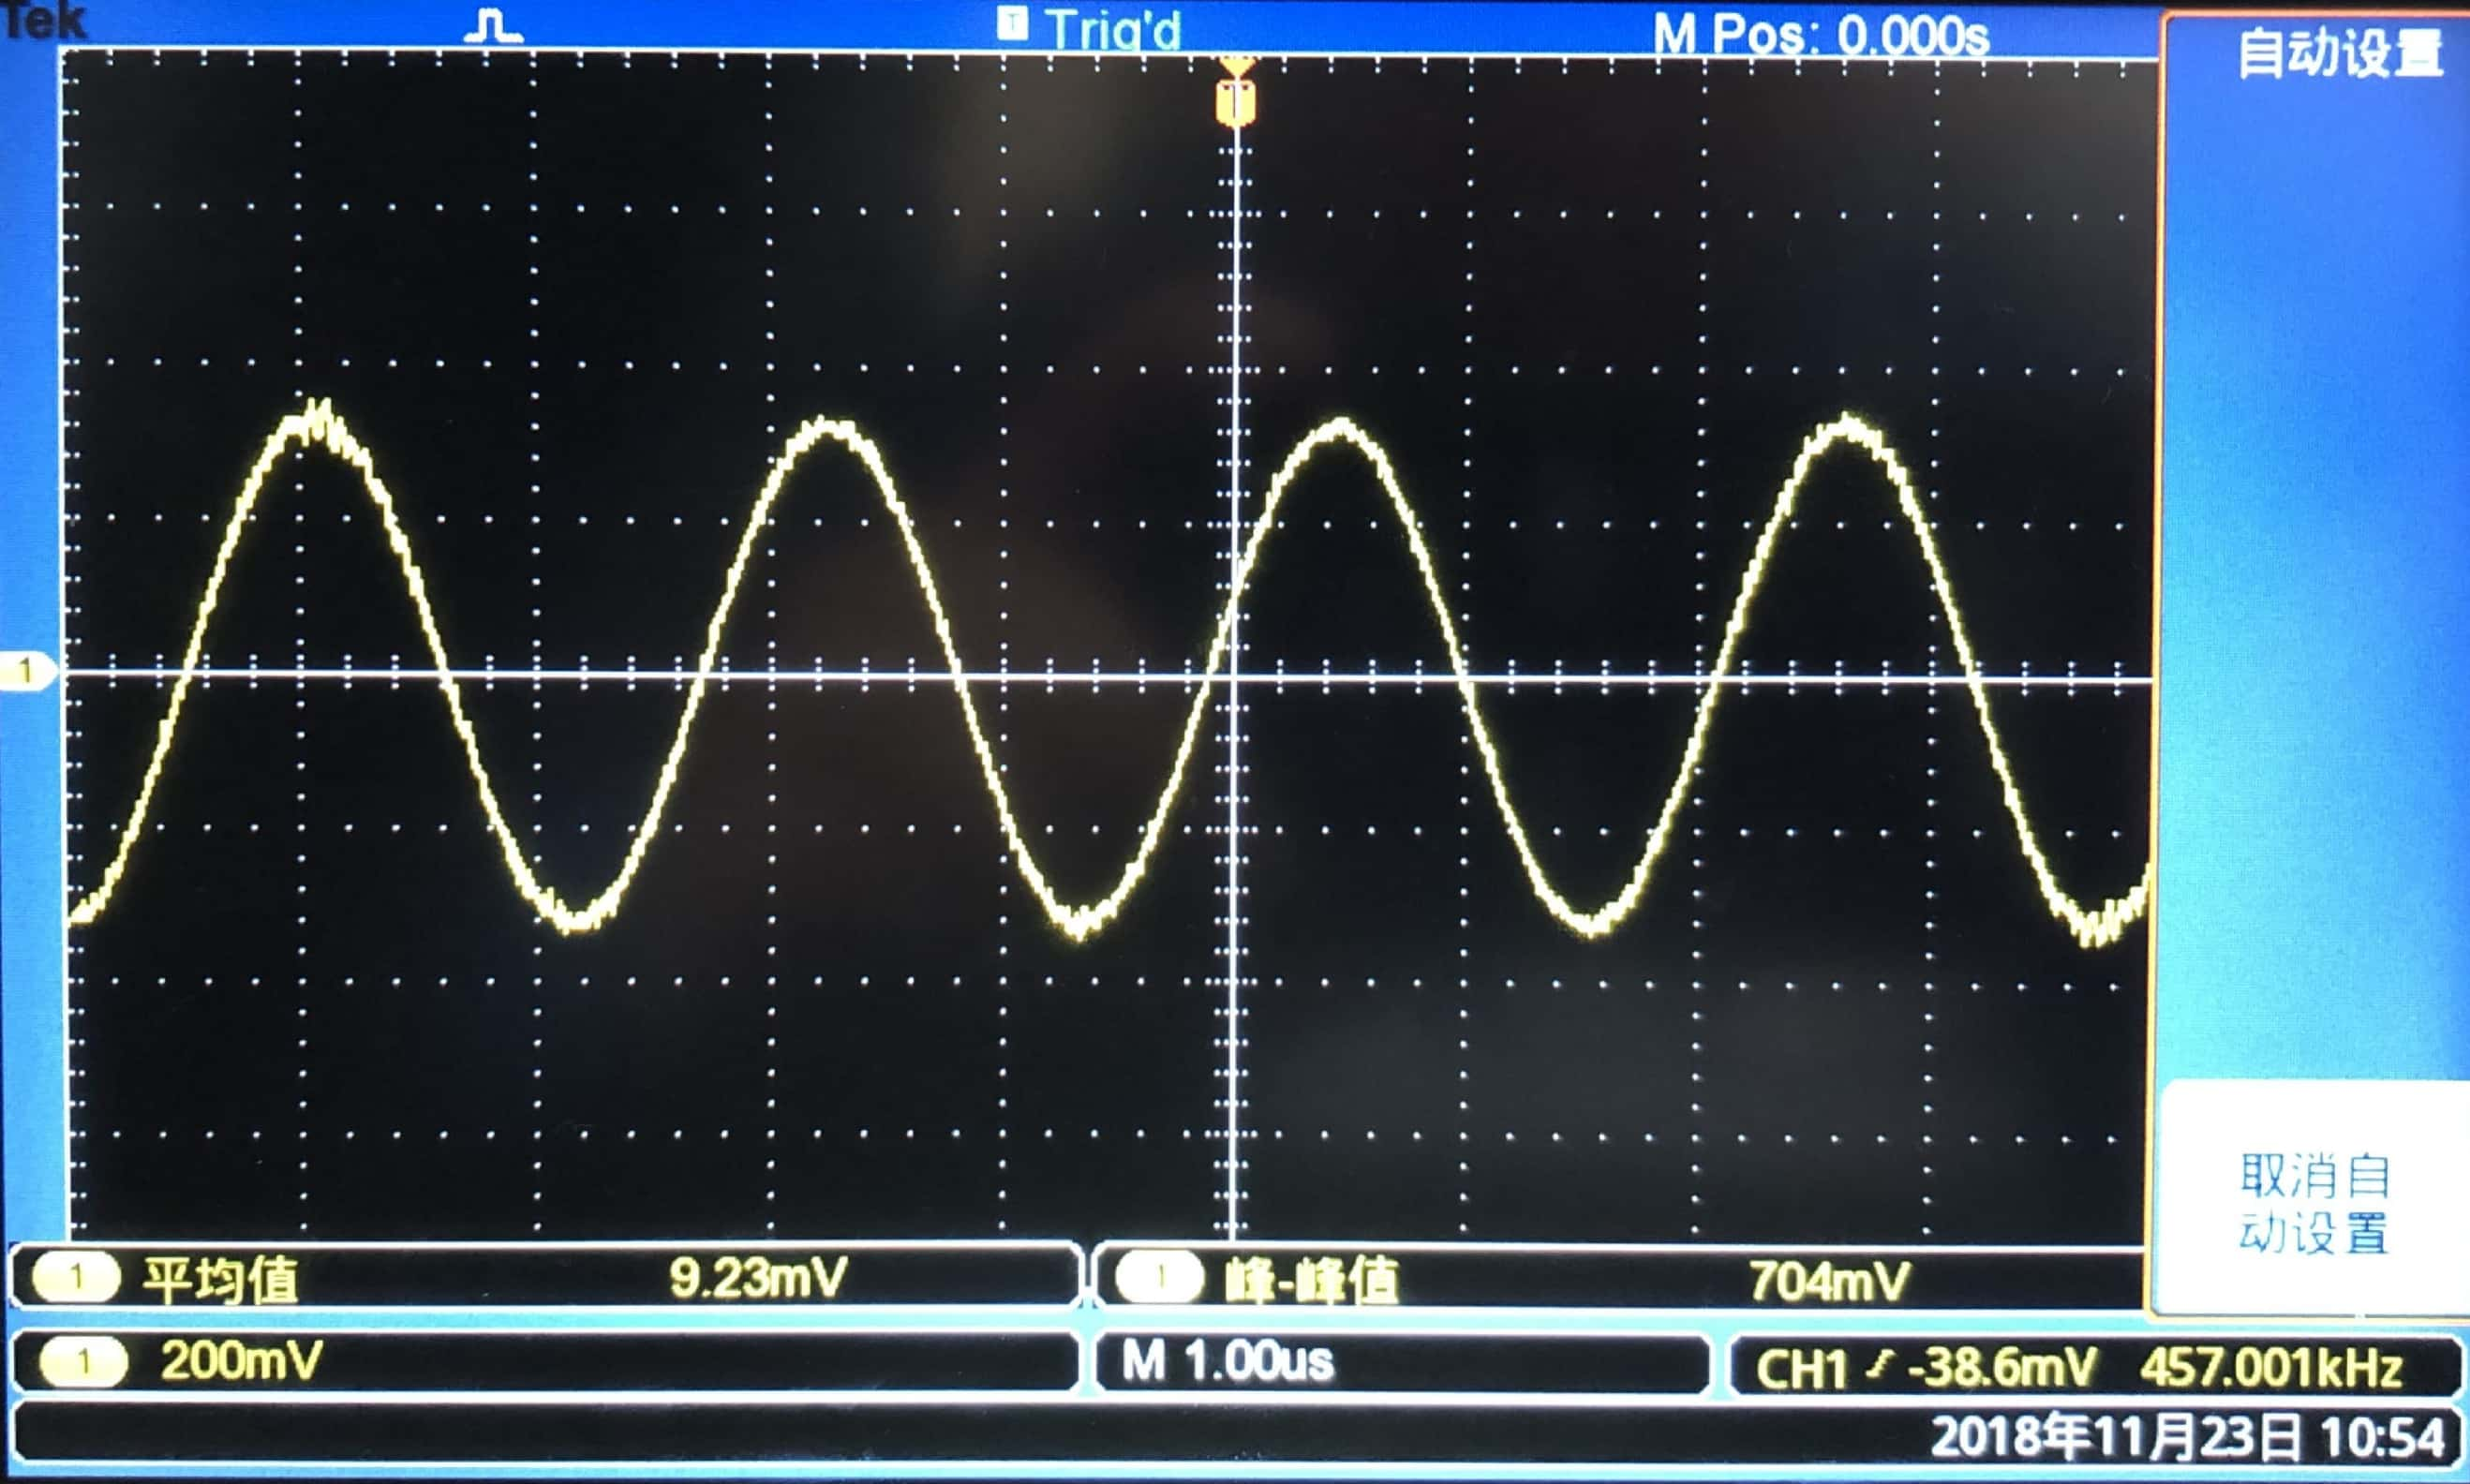
\includegraphics[width=0.35\textwidth]{gaopin2/gaopin202.jpg} &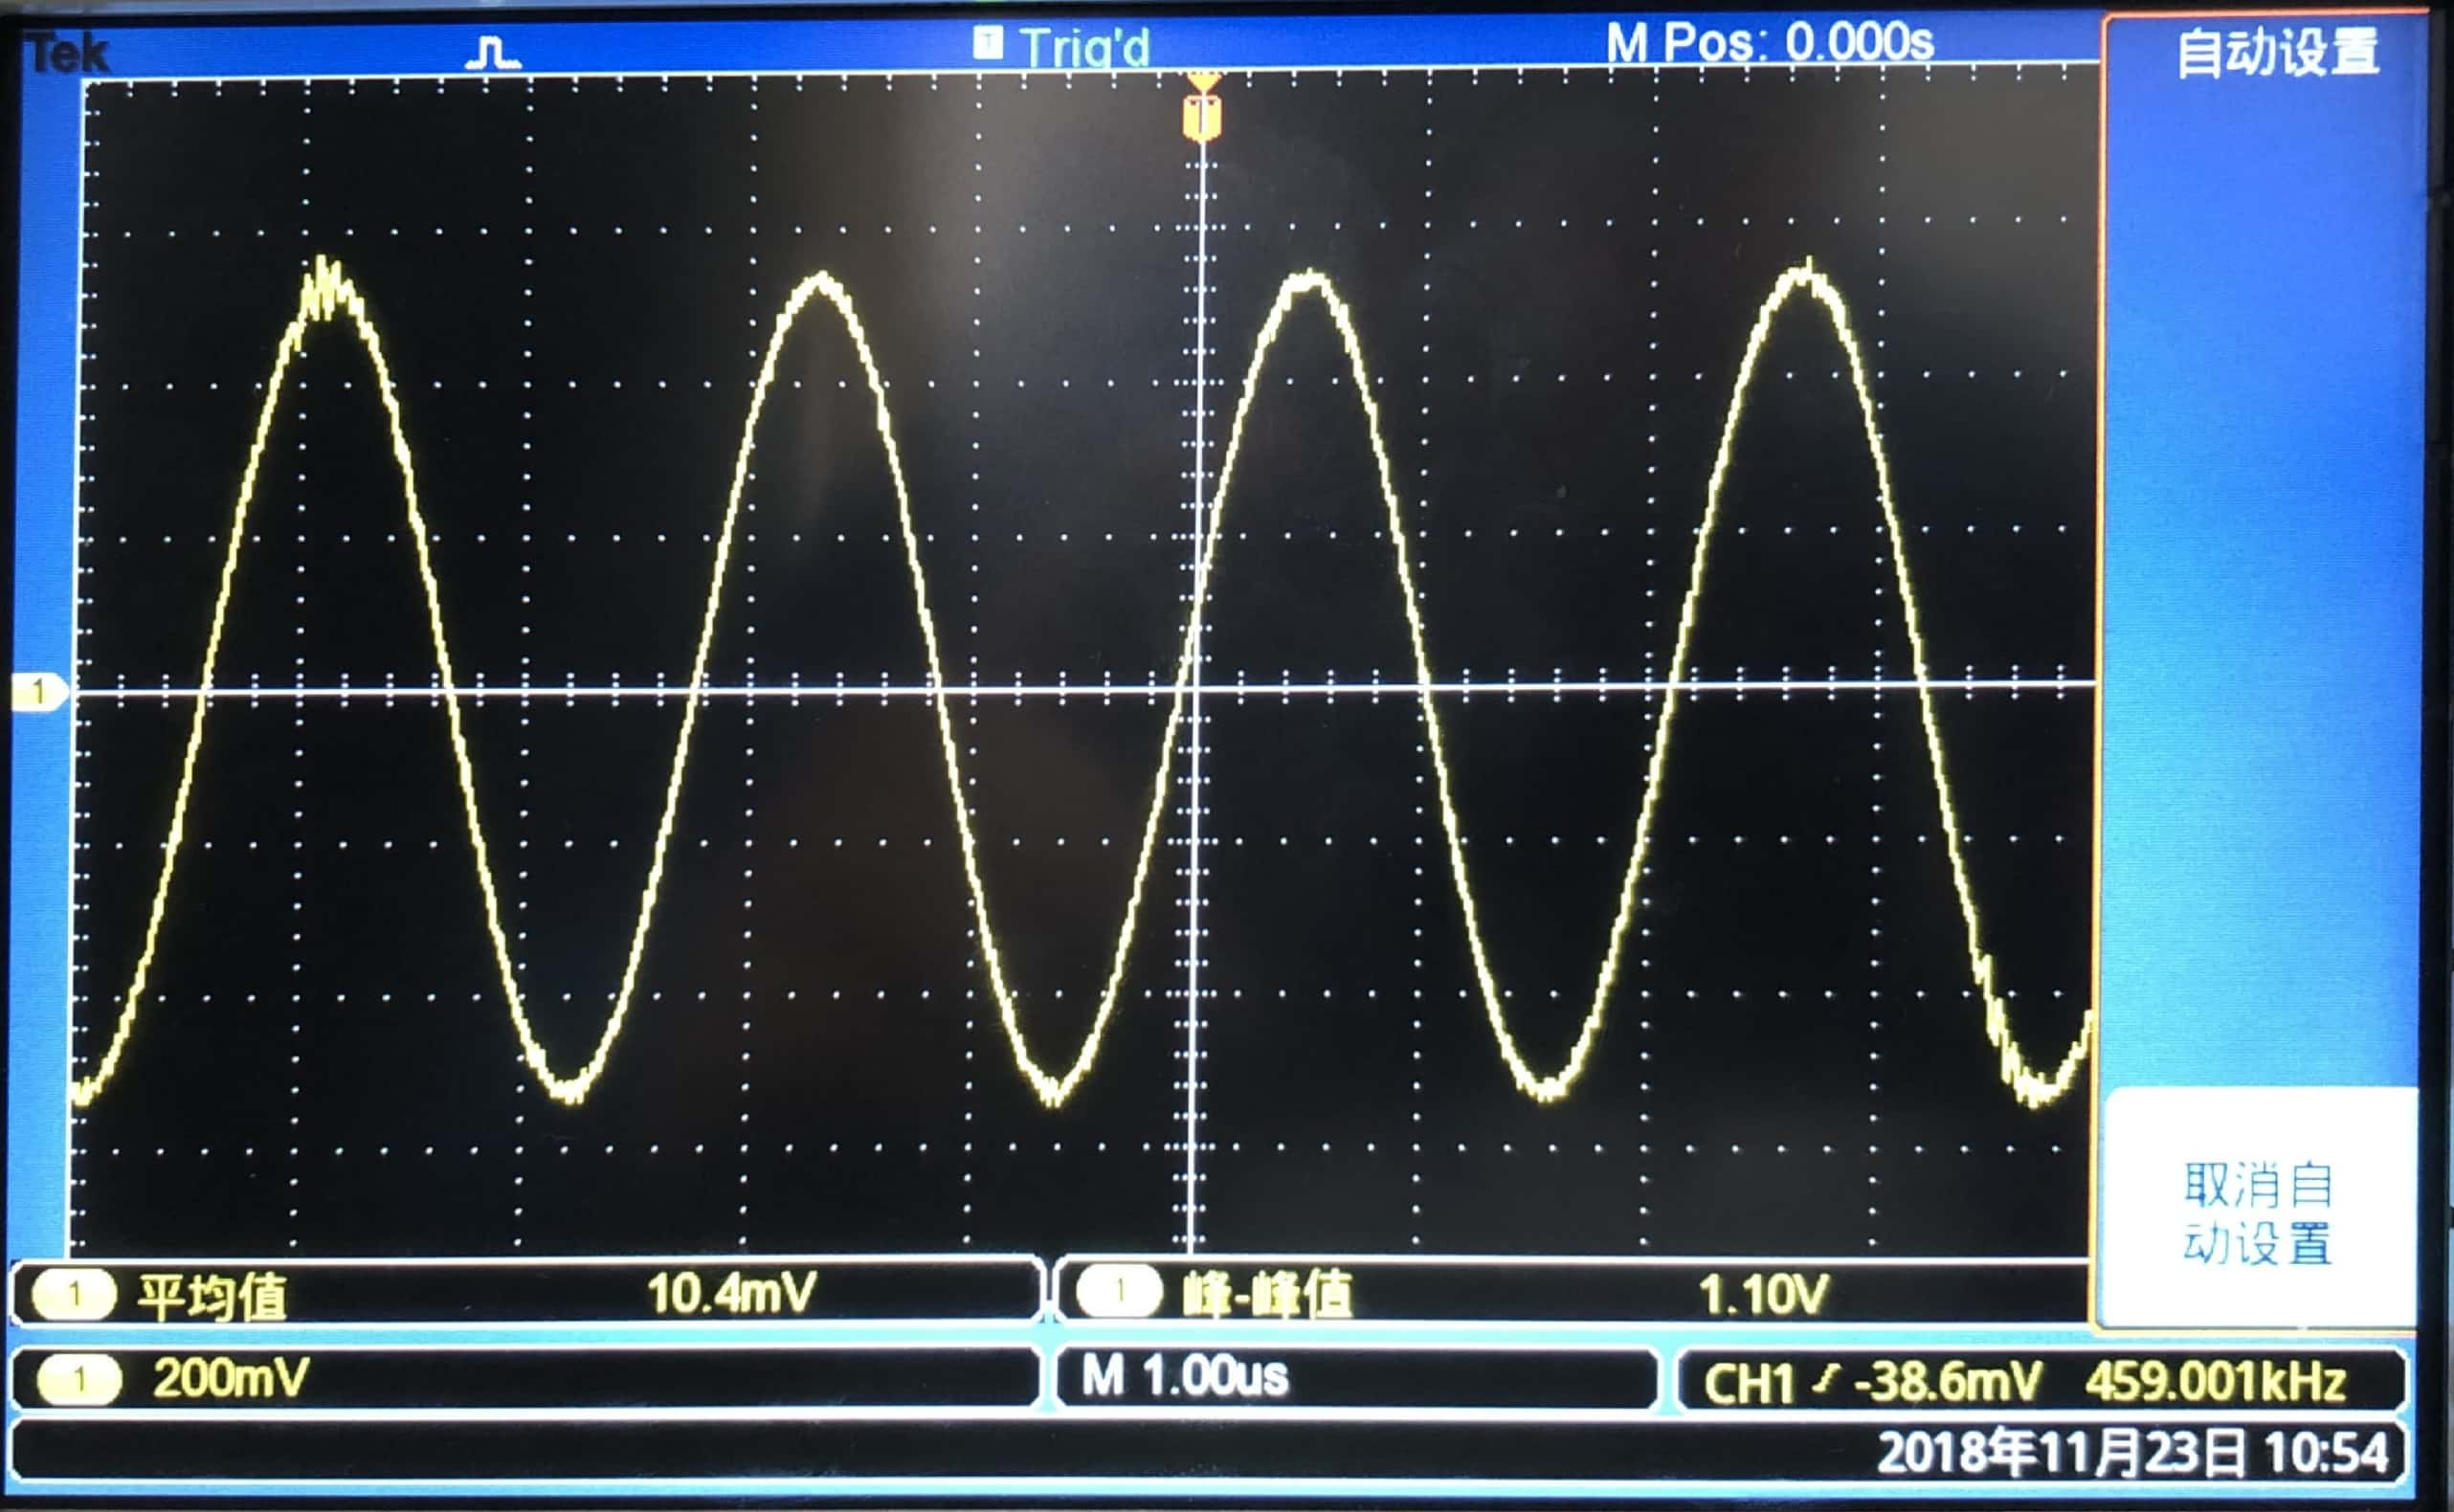
\includegraphics[width=0.35\textwidth]{gaopin2/gaopin222.jpg}&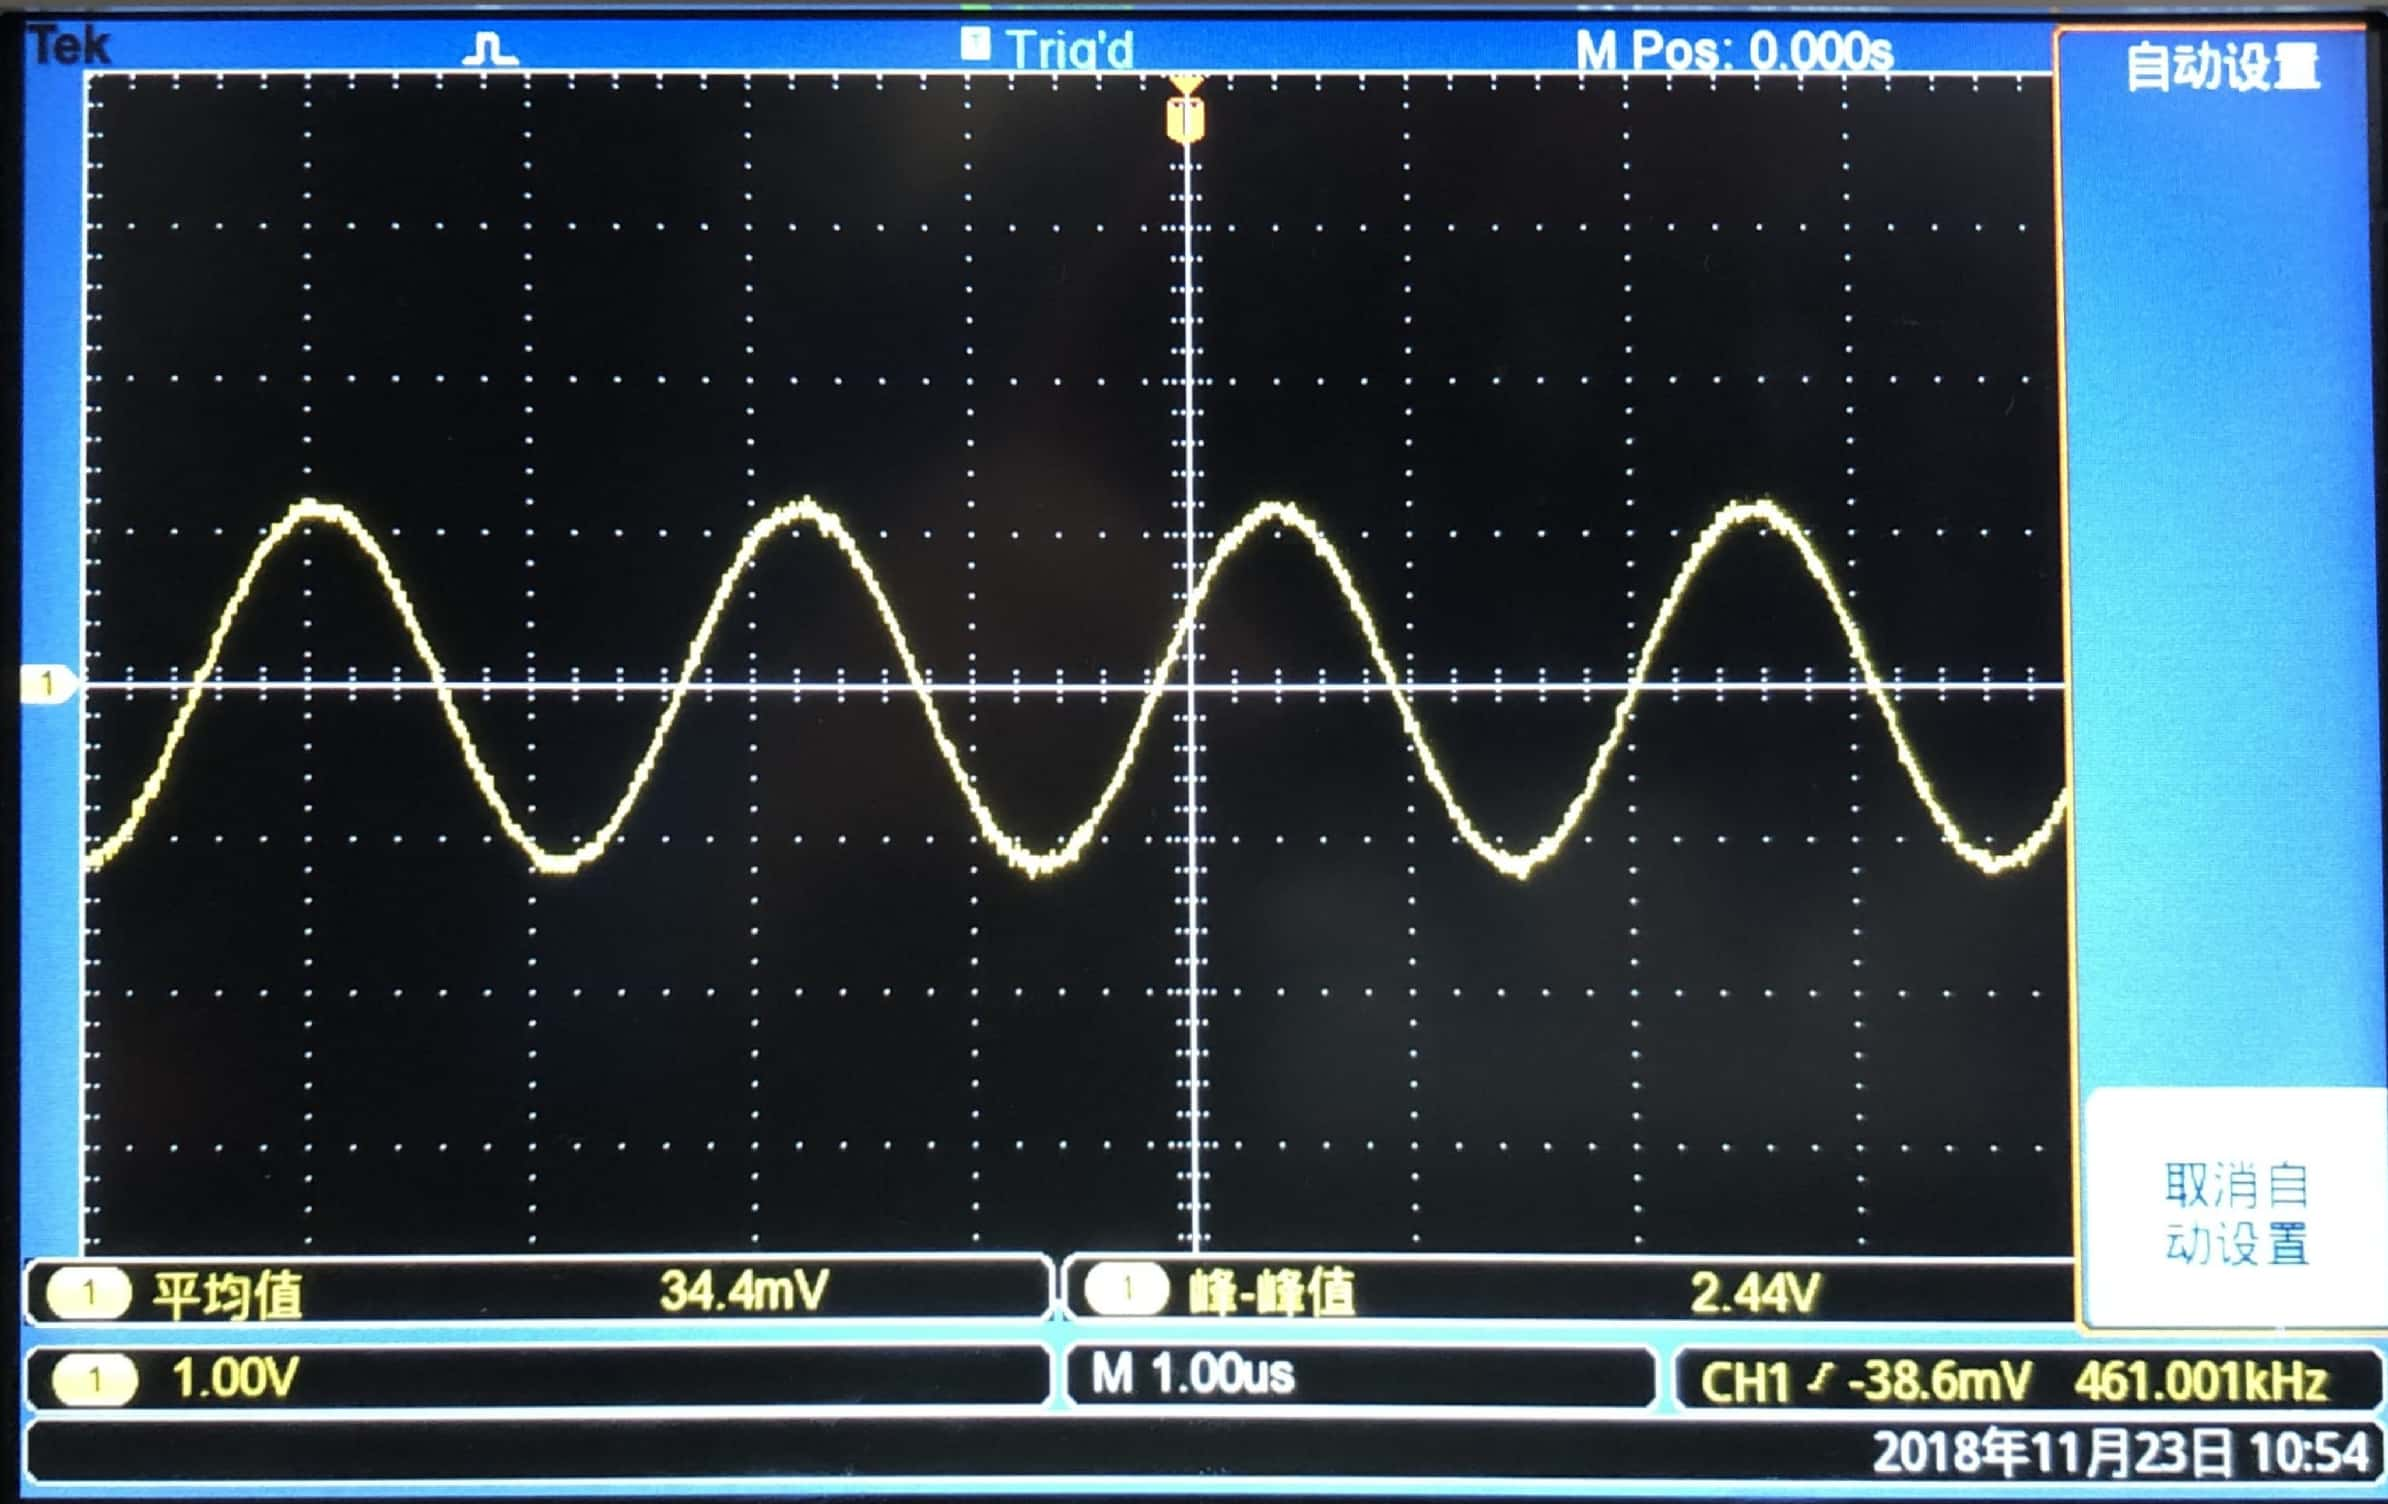
\includegraphics[width=0.35\textwidth]{gaopin2/gaopin204.jpg} \\ 
$f=457\ KHz$ & $f=459\ KHz$ & $f=461\ KHz$ \\
$V_o=704\ mv$ & $V_o=1.10\ v$ & $V_o=2.44\ v$ \\
\\
 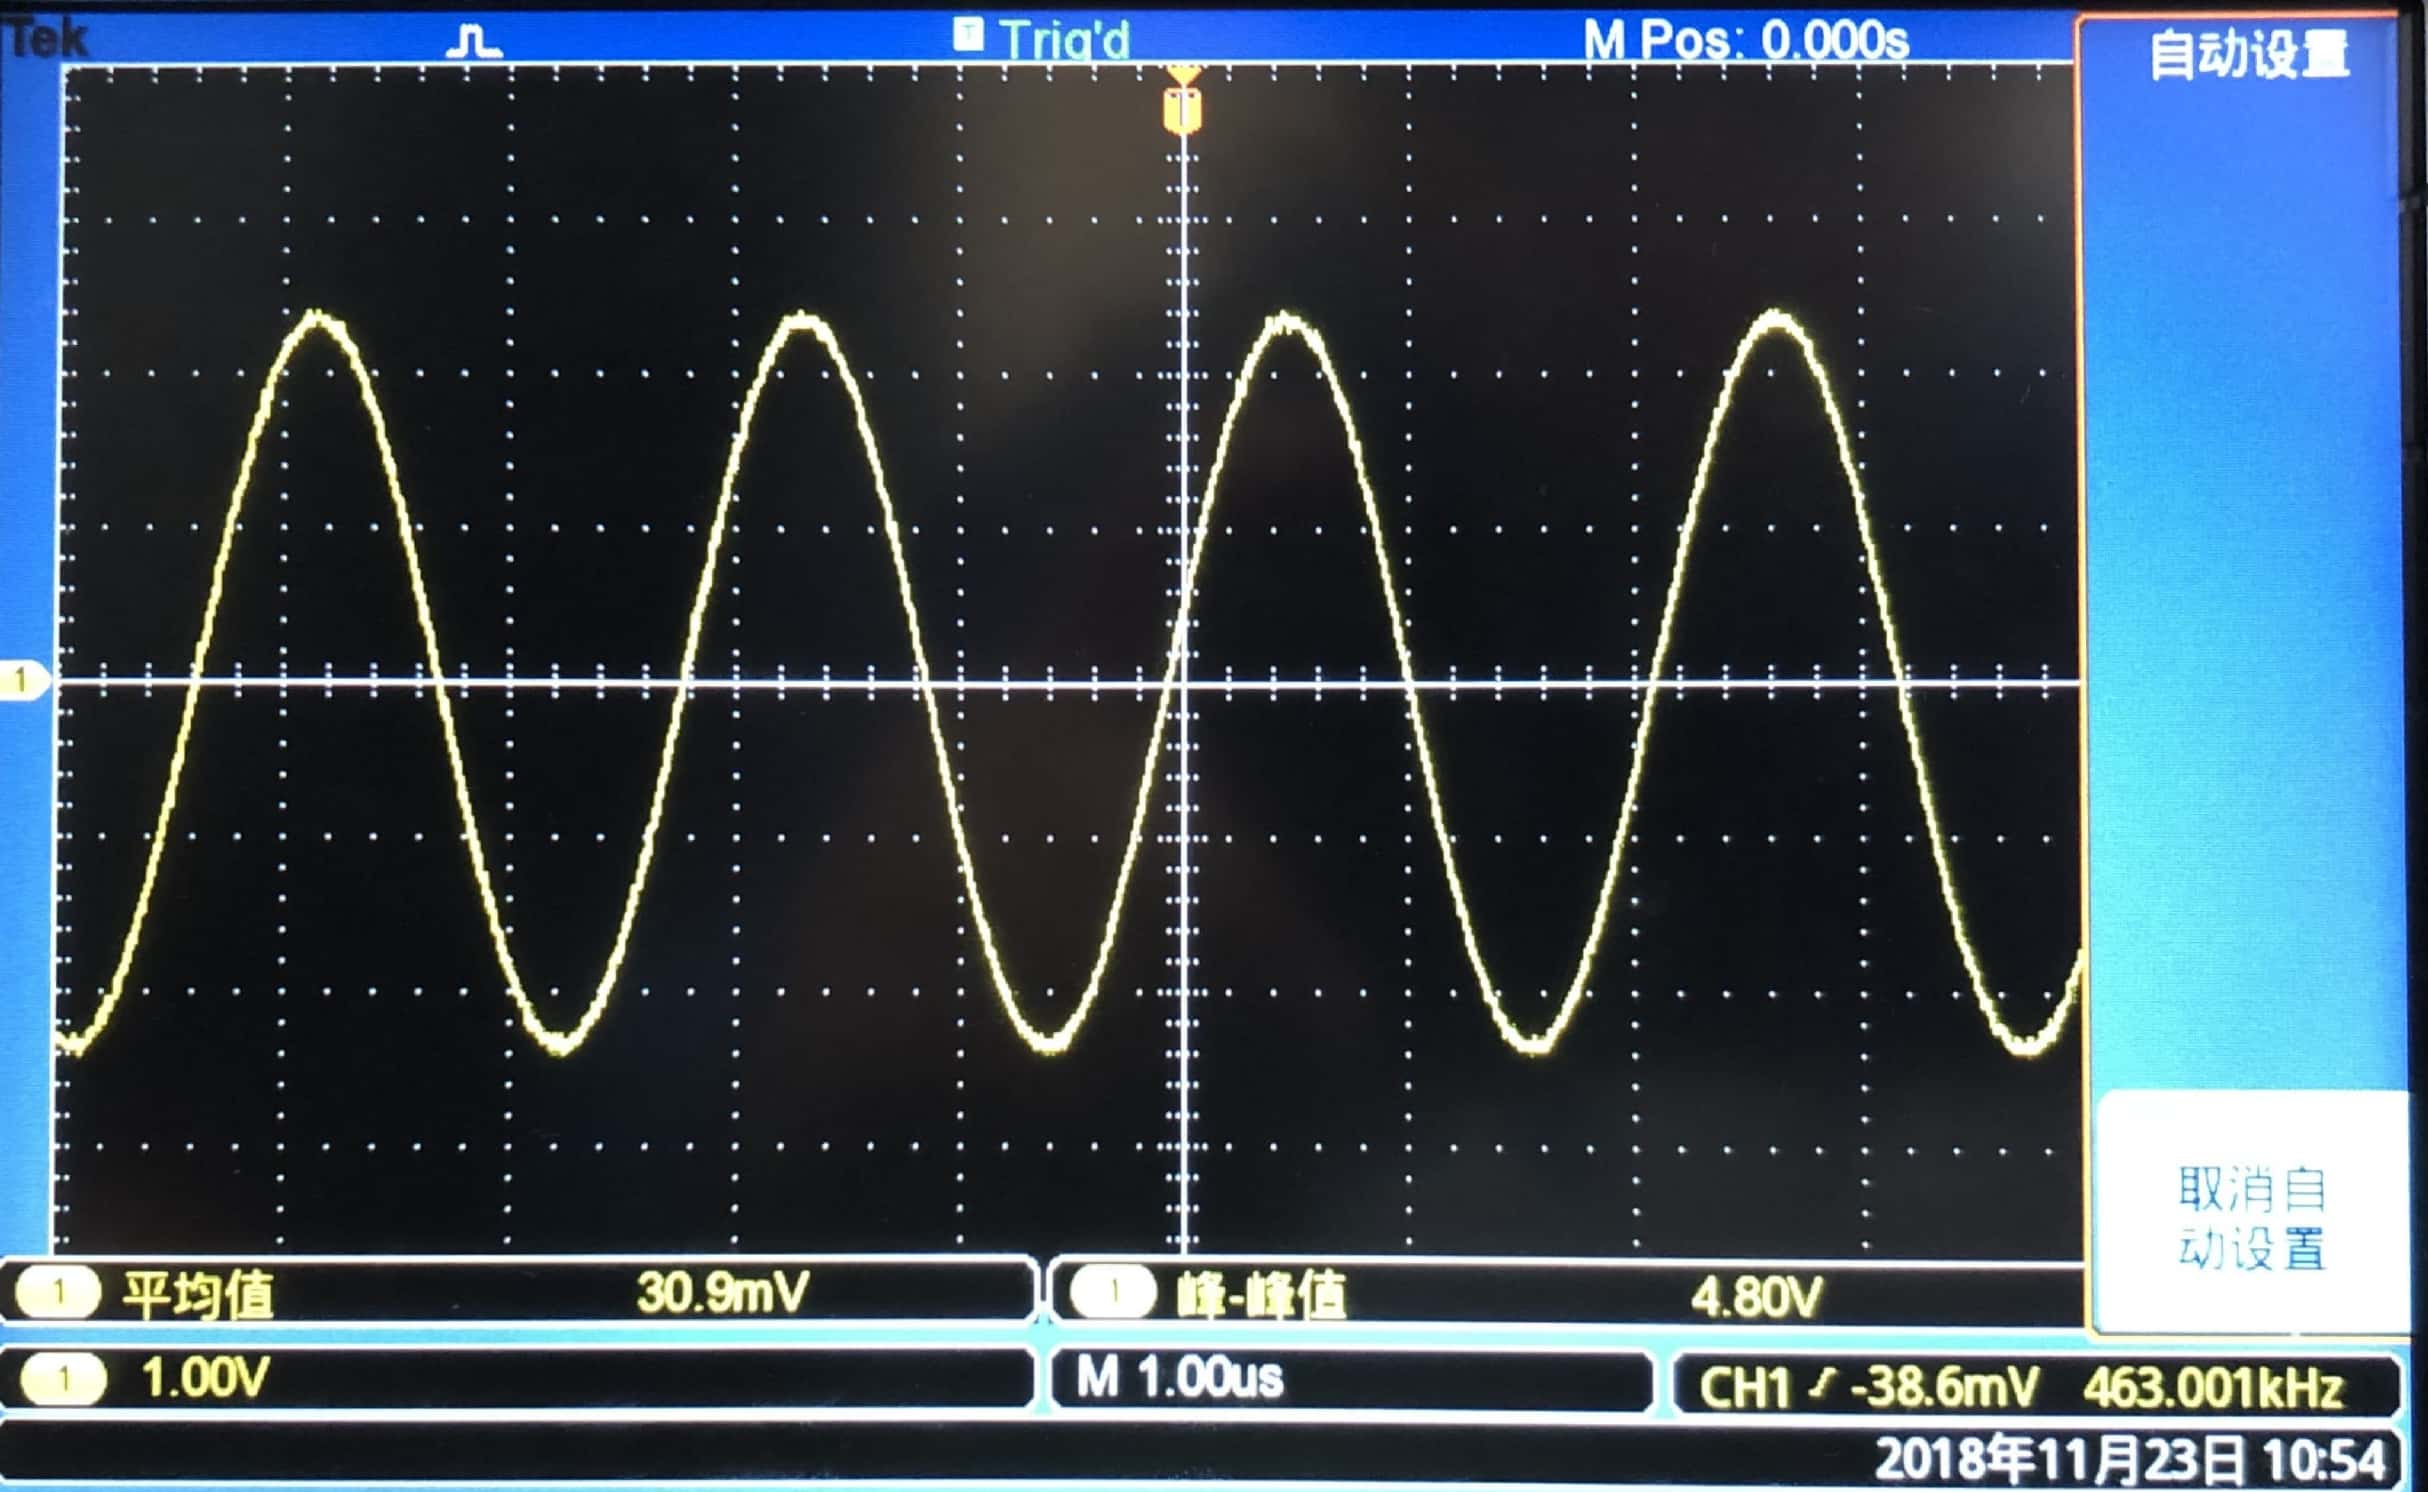
\includegraphics[width=0.35\textwidth]{gaopin2/gaopin210.jpg} &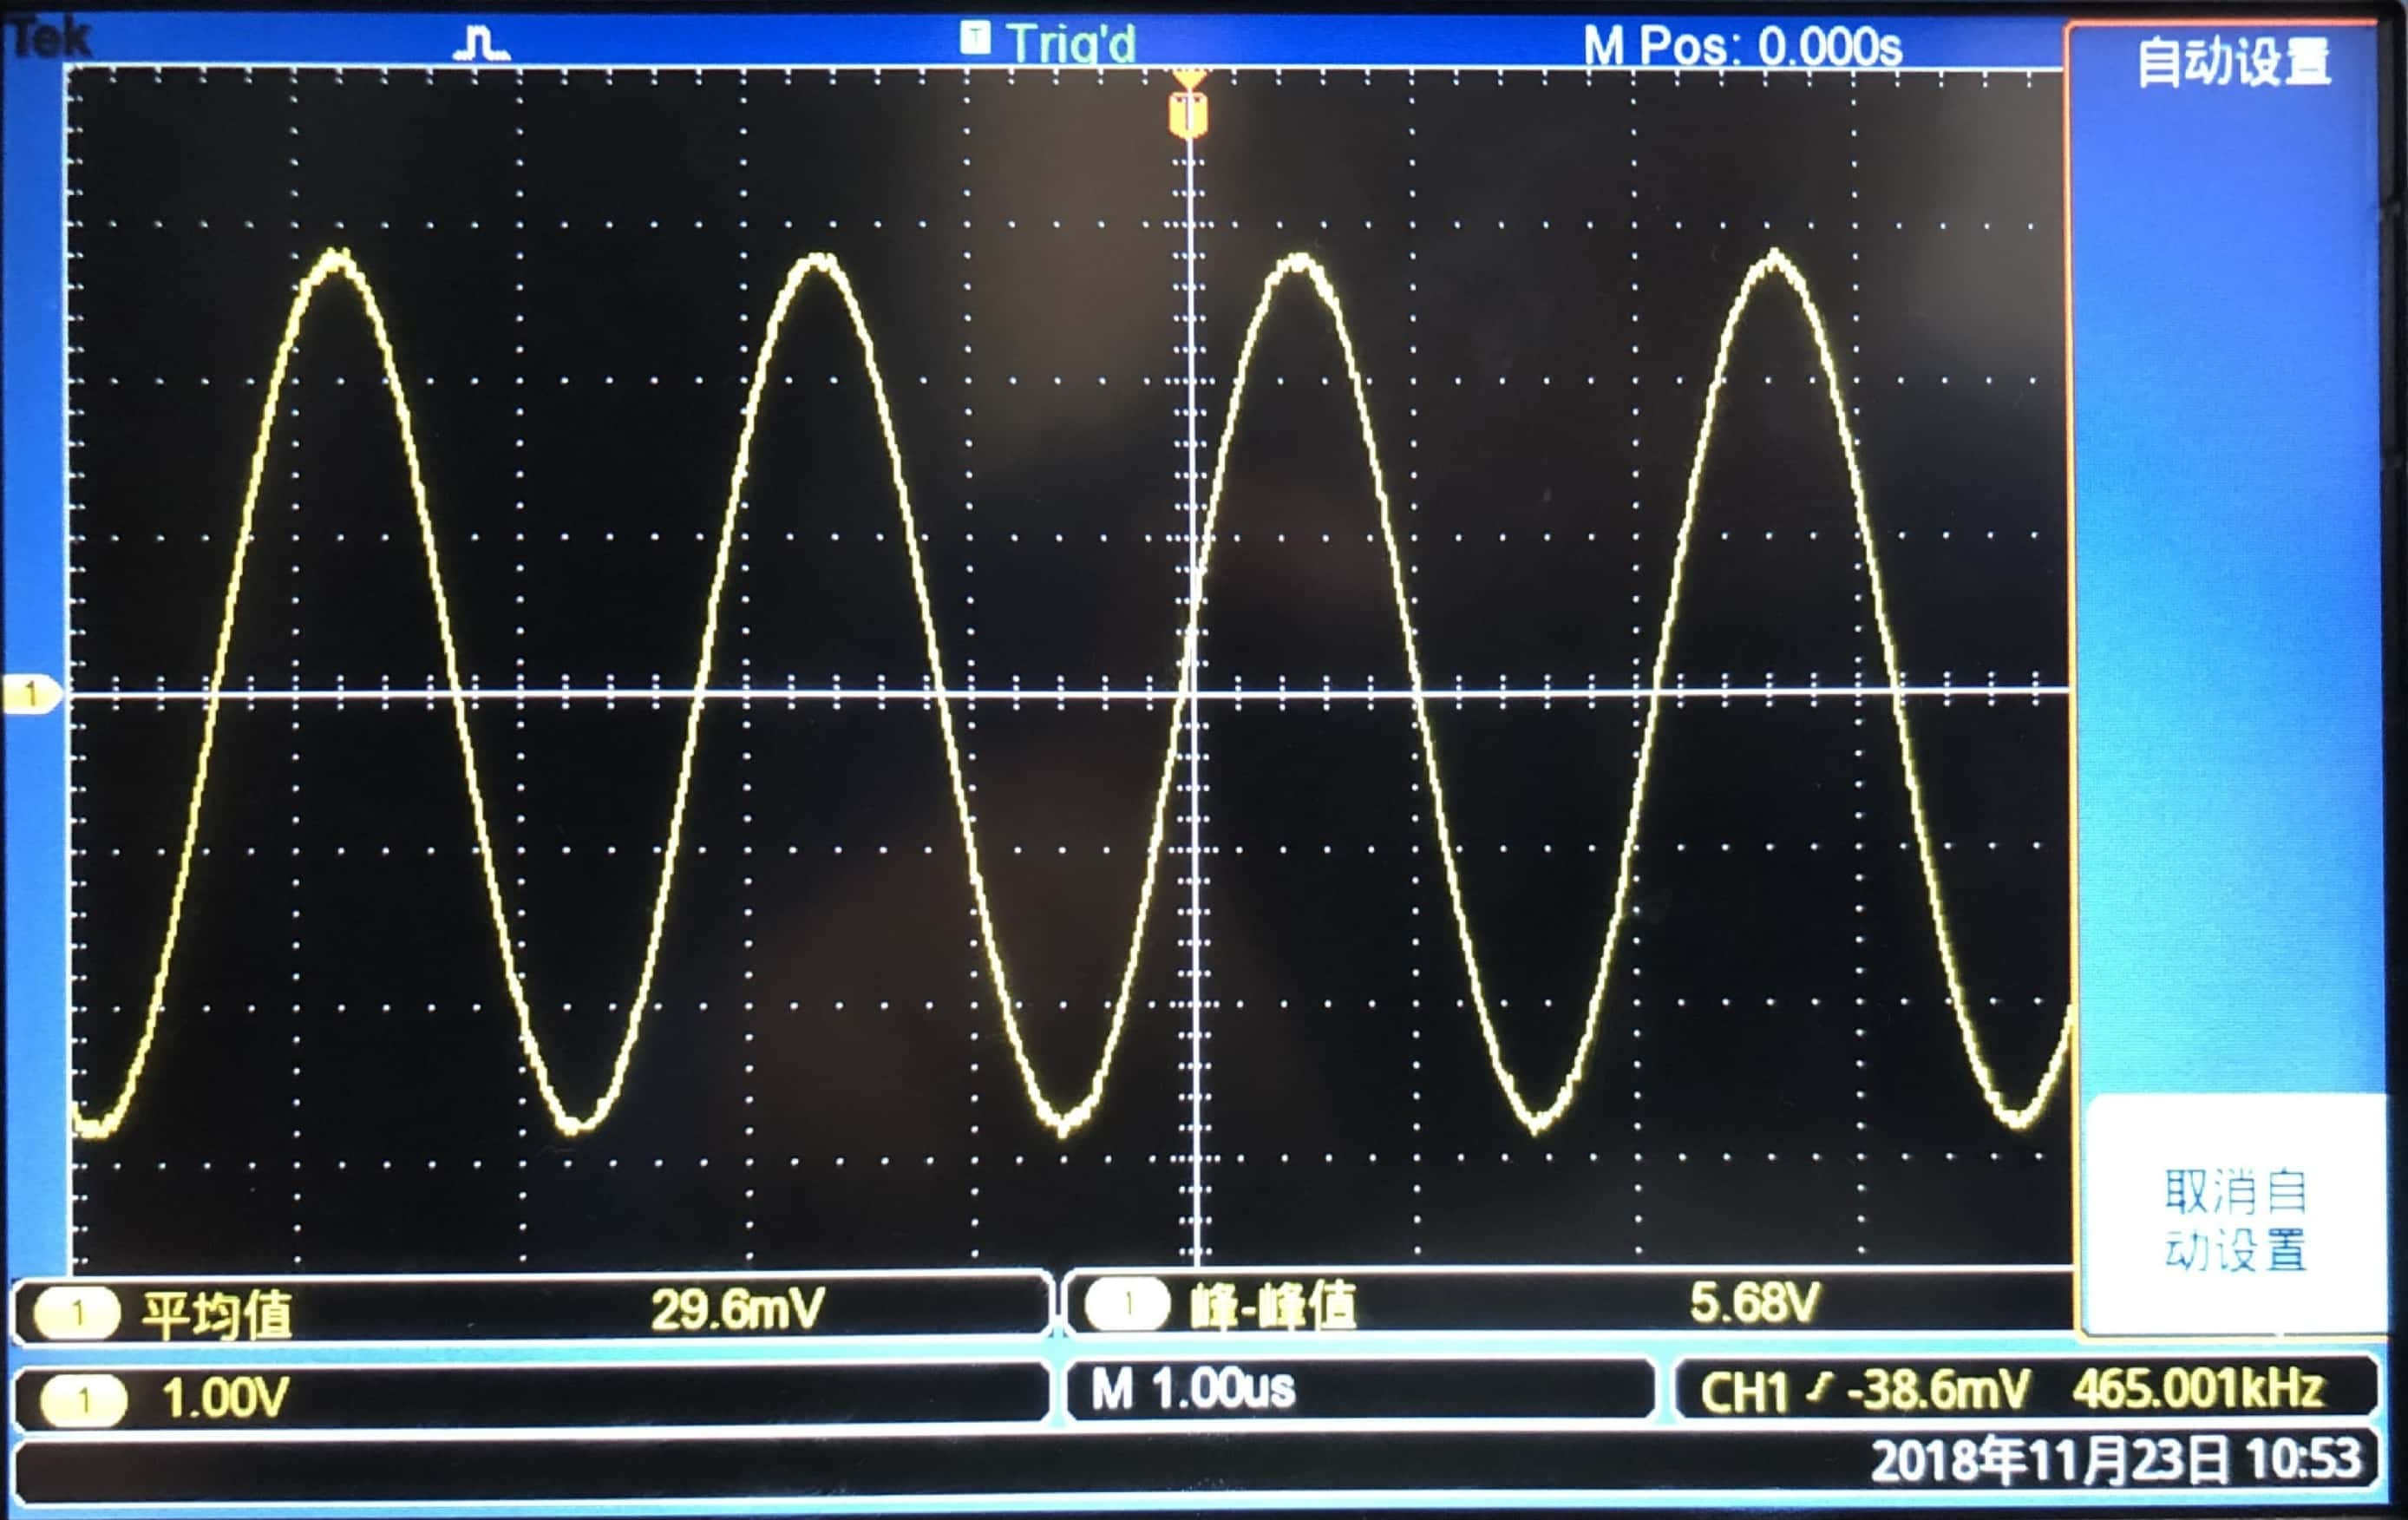
\includegraphics[width=0.35\textwidth]{gaopin2/gaopin216.jpg}&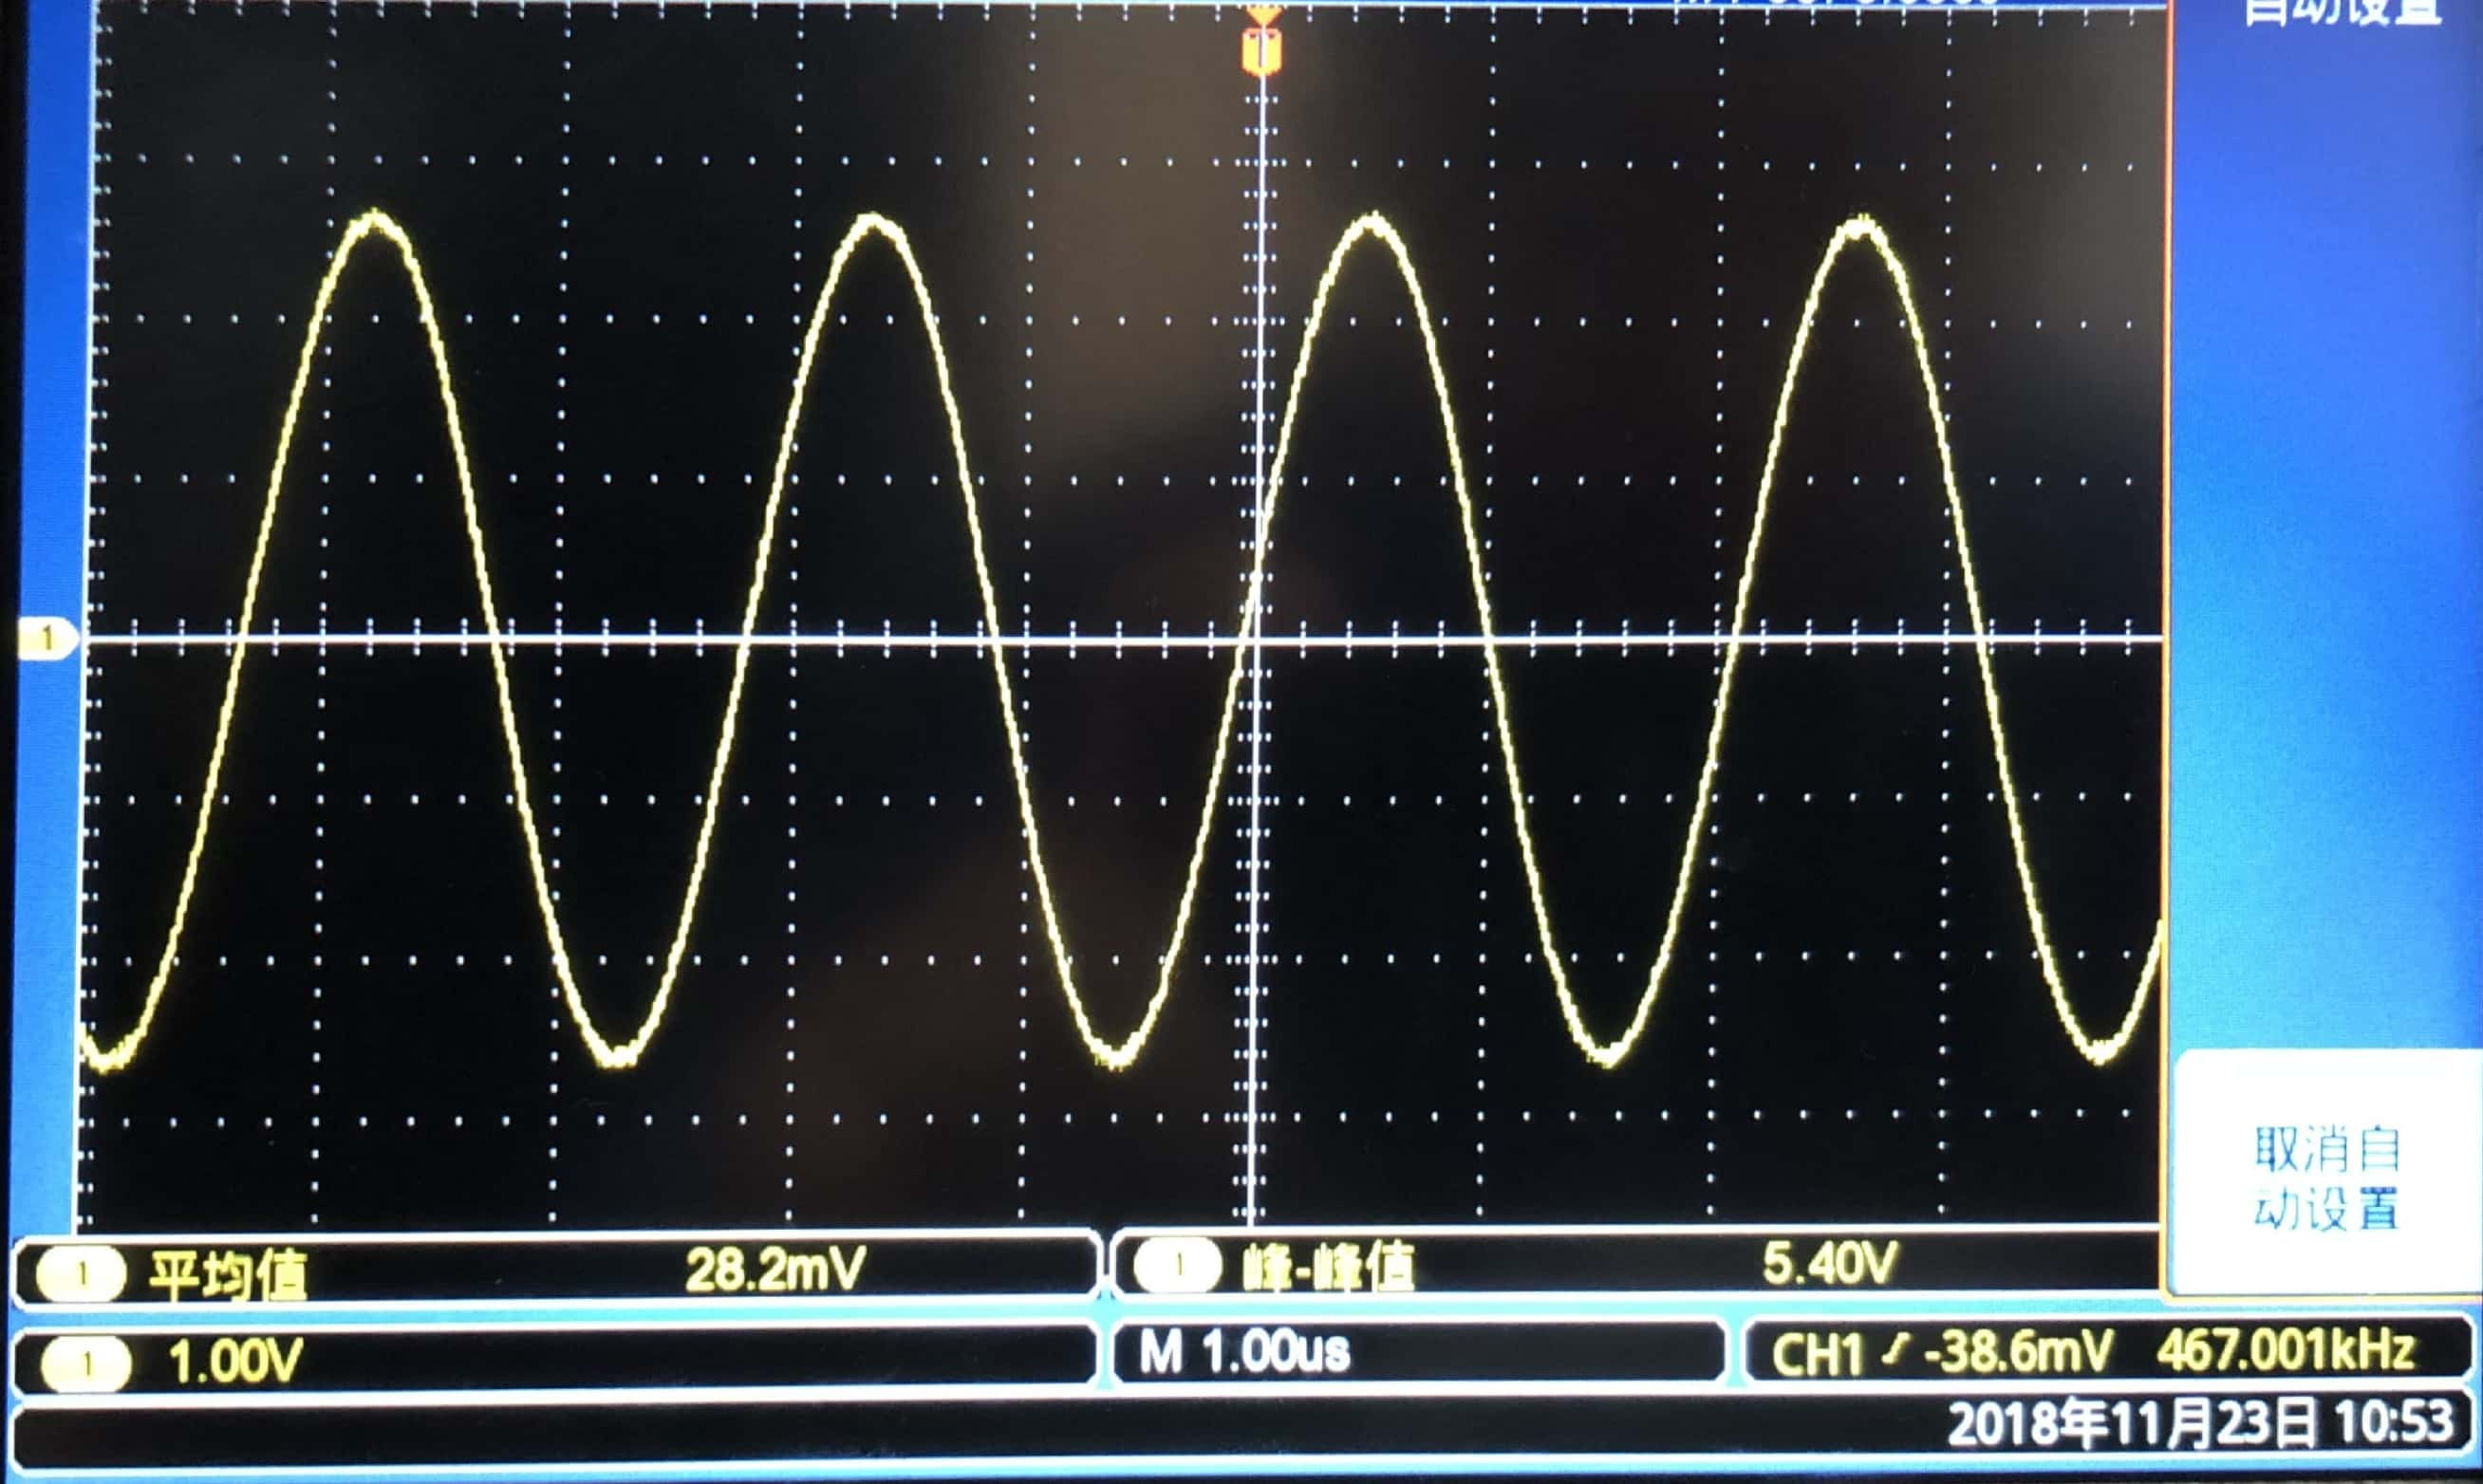
\includegraphics[width=0.35\textwidth]{gaopin2/gaopin211.jpg} \\ 
$f=463\ KHz$ & $f=465\ KHz$ & $f=467\ KHz$ \\
$V_o=4.80\ v$ & $V_o=5.68\ v$ & $V_o=5.40\ v$ \\
\\
 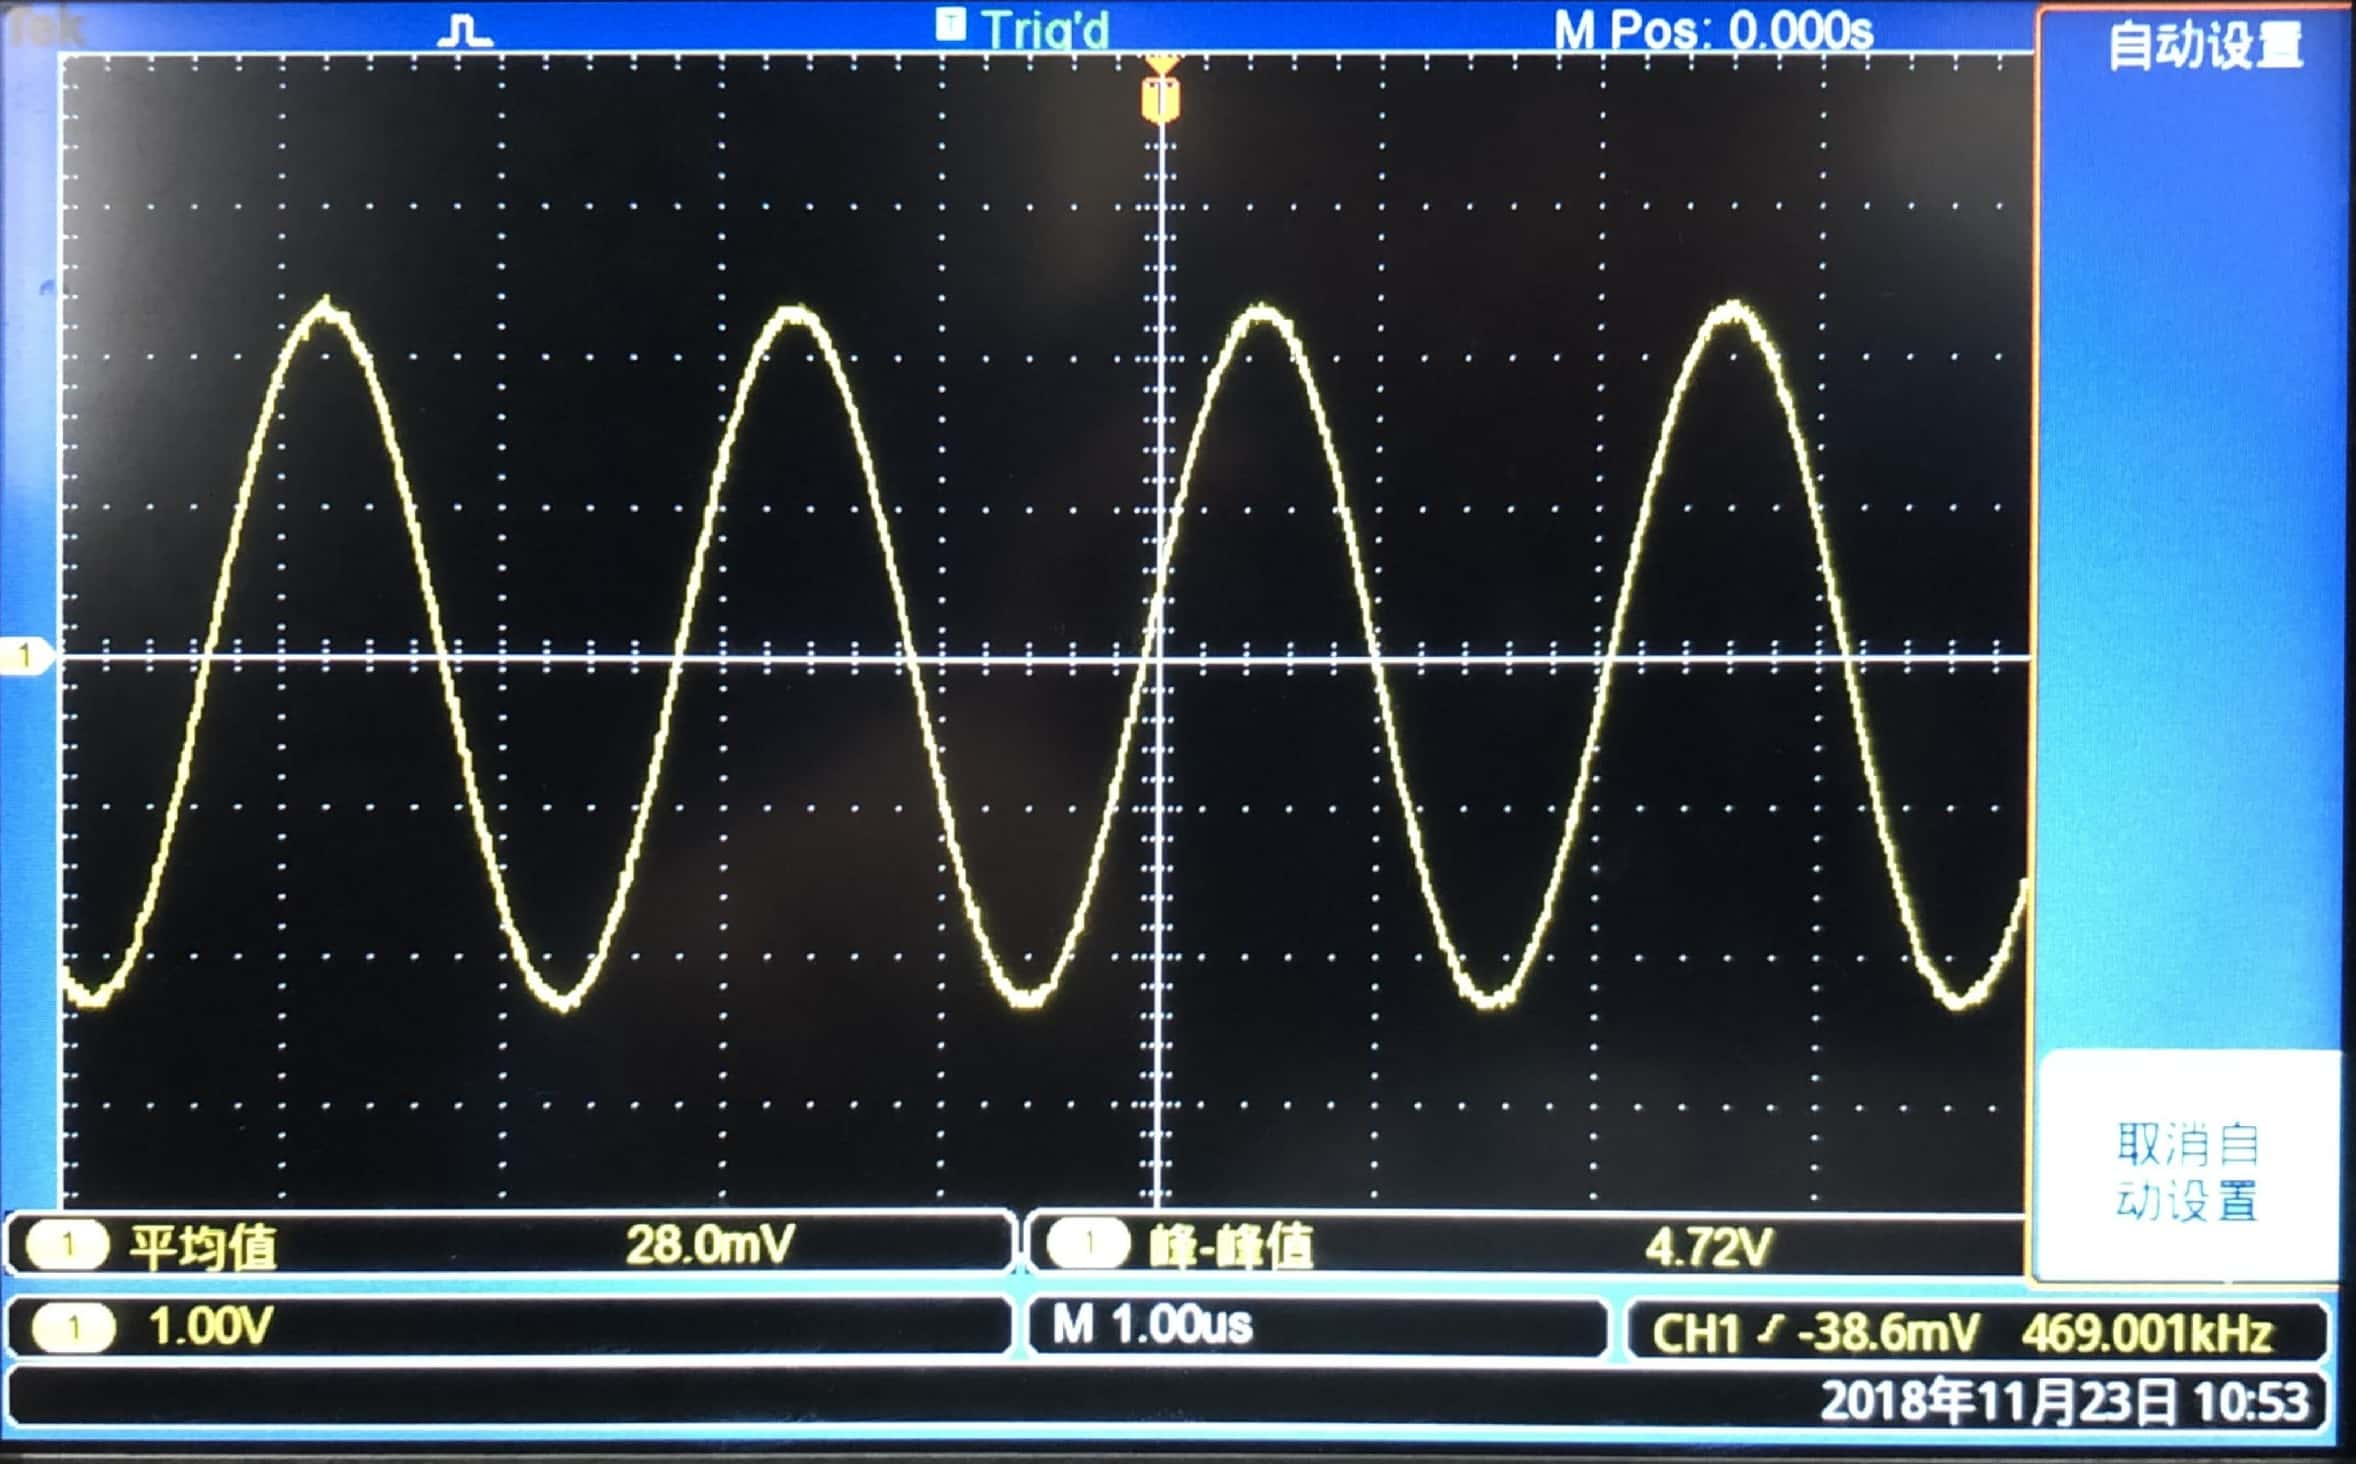
\includegraphics[width=0.35\textwidth]{gaopin2/gaopin207.jpg} &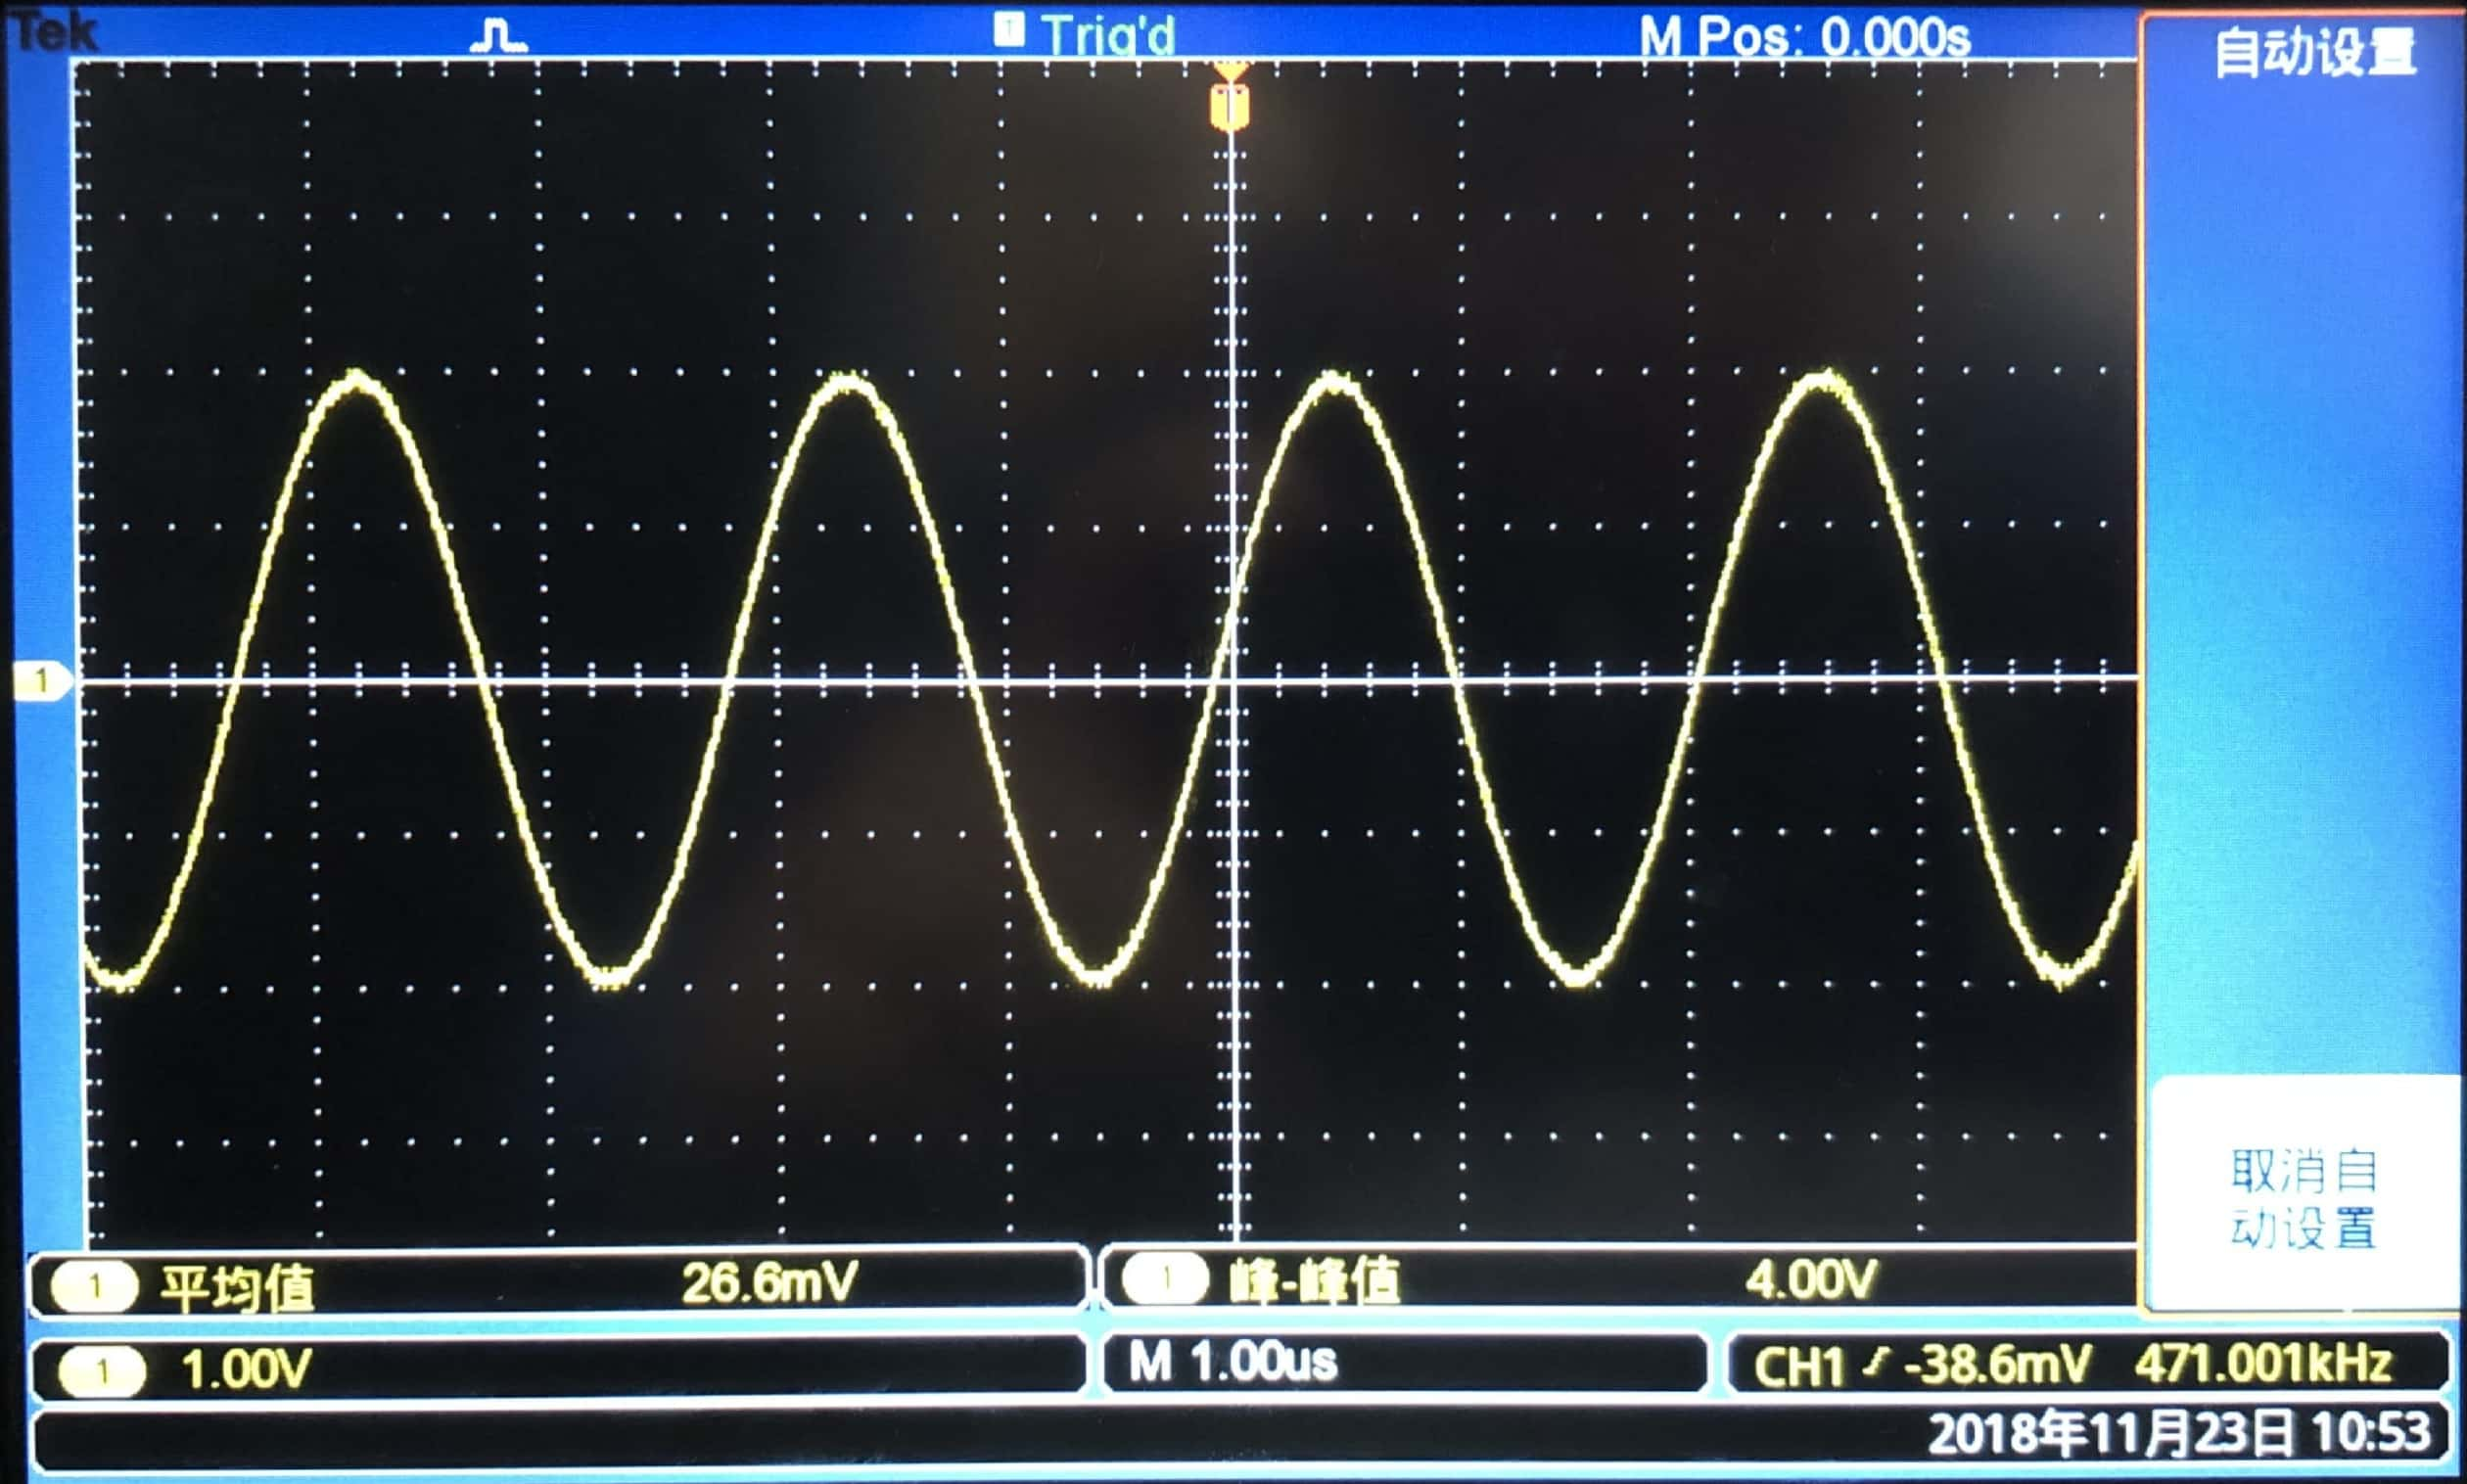
\includegraphics[width=0.35\textwidth]{gaopin2/gaopin205.jpg}&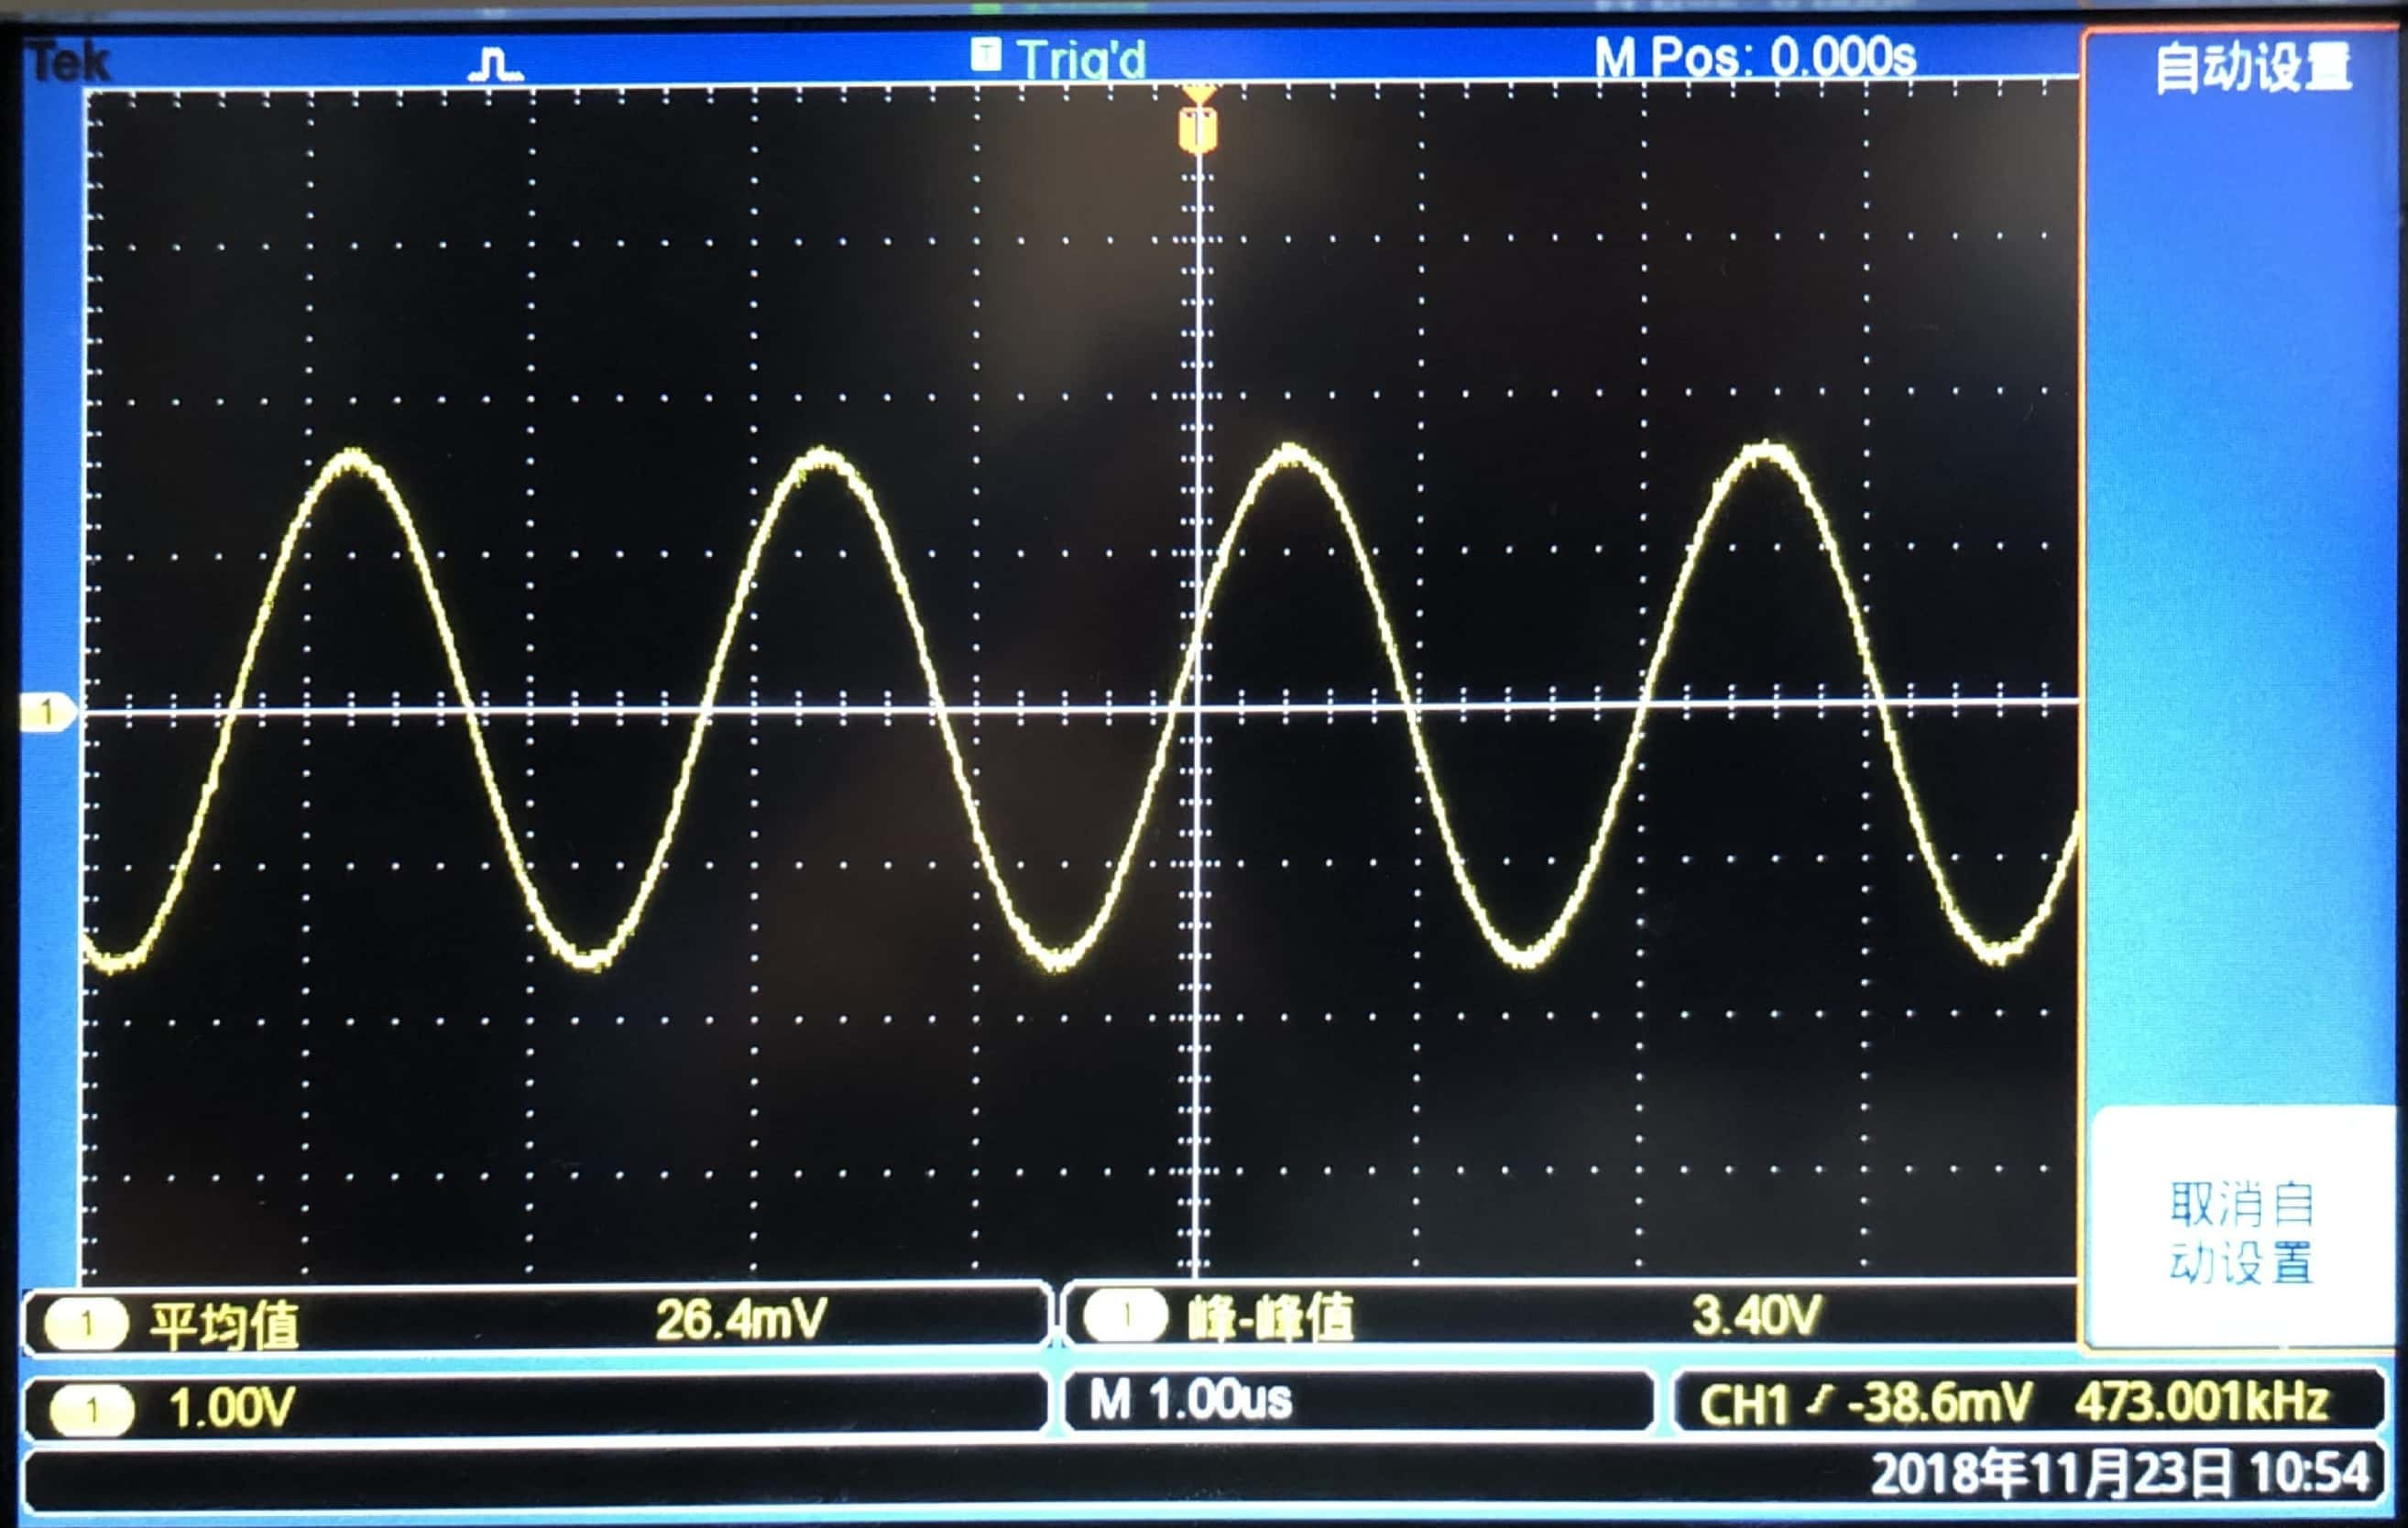
\includegraphics[width=0.35\textwidth]{gaopin2/gaopin203.jpg} \\ 
$f=469\ KHz$ & $f=471\ KHz$ & $f=473\ KHz$ \\
$V_o=4.72\ v$ & $V_o=4.00\ v$ & $V_o=3.40\ v$ \\
\end{tabular}
\caption{双调谐小信号放大器输出信号波形图}\label{img:122}
\end{figure}
\end{enumerate}
\section{模拟乘法混频(模块2)}
\setcounter{equation}{0}
\setcounter{table}{0}
\setcounter{figure}{0}
\subsection{实验目的}
\begin{enumerate}\addtolength{\itemsep}{-1.5ex}
\item 了解集成混频器的工作原理
\item 了解混频器中的寄生干扰
\end{enumerate}
\subsection{实验原理及实验电路说明}\label{yl:hunpin}
在高频电子电路中,常常需要将信号自某一频率变成另一个频率。这样不仅能满足各种无线电设备的需要,而且有利于提高设备的性能。对信号进行变频,是将信号的各分量移至新的频域,各分量的频率间隔和相对幅度保持不变。进行这种频率变换时,新频率等于信号原来的频率与某一参考频率之和或差。该参考频率通常称为本机振荡频率。本机振荡频率可以是由单独的信号源供给,也可以由频率变换电路内部产生。当本机振荡由单独的信号源供给时,这样的频率变换电路称为混频器。\par
混频器常用的非线性器件有二极管、三极管、场效应管和乘法器。本振用于产生一个等幅的高频信号VL,并与输入信号 VS经混频器后所产生的差频信号经带通滤波器滤出。\par
本实验采用集成模拟相乘器作混频电路实验。\par
因为模拟相乘器的输出频率包含有两个输入频率之差或和,故模拟相乘器加滤波器,滤波器滤除不需要的分量,取和频或者差频二者之一,即构成混频器。\par
     图\ref{img:cfh}所示为相乘混频器的方框图。设滤波器滤除和频,则输出差频信号。图\ref{img:cfhg}为信号经混频前后的频谱图。我们设信号是:载波频率为$f_S$的普通调幅波。本机振荡频率为$f_L$。\par
       \begin{figure}[ht]
  \centering
  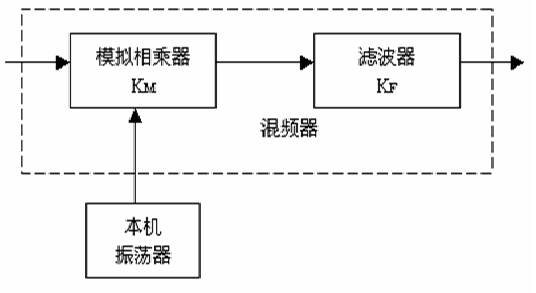
\includegraphics[width=0.5\textwidth]{image009.png} 
  \caption{ 相乘混频方框图} 
  \label{img:cfh} 
\end{figure}
       \begin{figure}[ht]
  \centering
  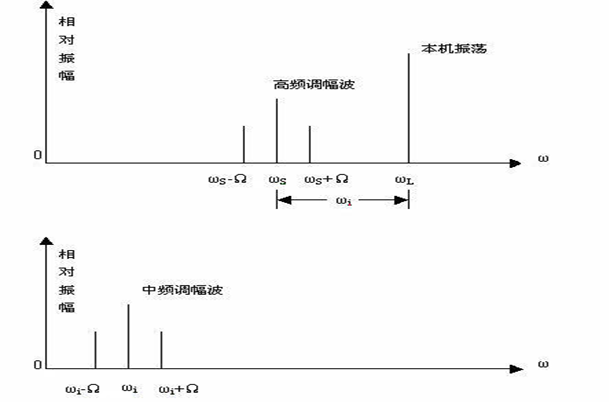
\includegraphics[width=.8\textwidth]{image010.png} 
  \caption{ 混频前后频谱图} 
  \label{img:cfhg} 
\end{figure}
    图\ref{img:cfhi}为模拟乘法器混频电路,该电路由集成模拟乘法器MC1496完成。MC1496可以采用单电源供电,也可采用双电源供电。本实验电路中采用+12V,-8V供电。$R_{22}$(820$\Omega$)、$R_{23}$(820$\Omega$)组成平衡电路,$F_2$为4.5MHz选频回路。本实验中输入信号频率为$f_S=4.2MHz$,本振频率$f_L=8.7MHz$,分别从J3,J4口输入。
       \begin{figure}[ht]
  \centering
  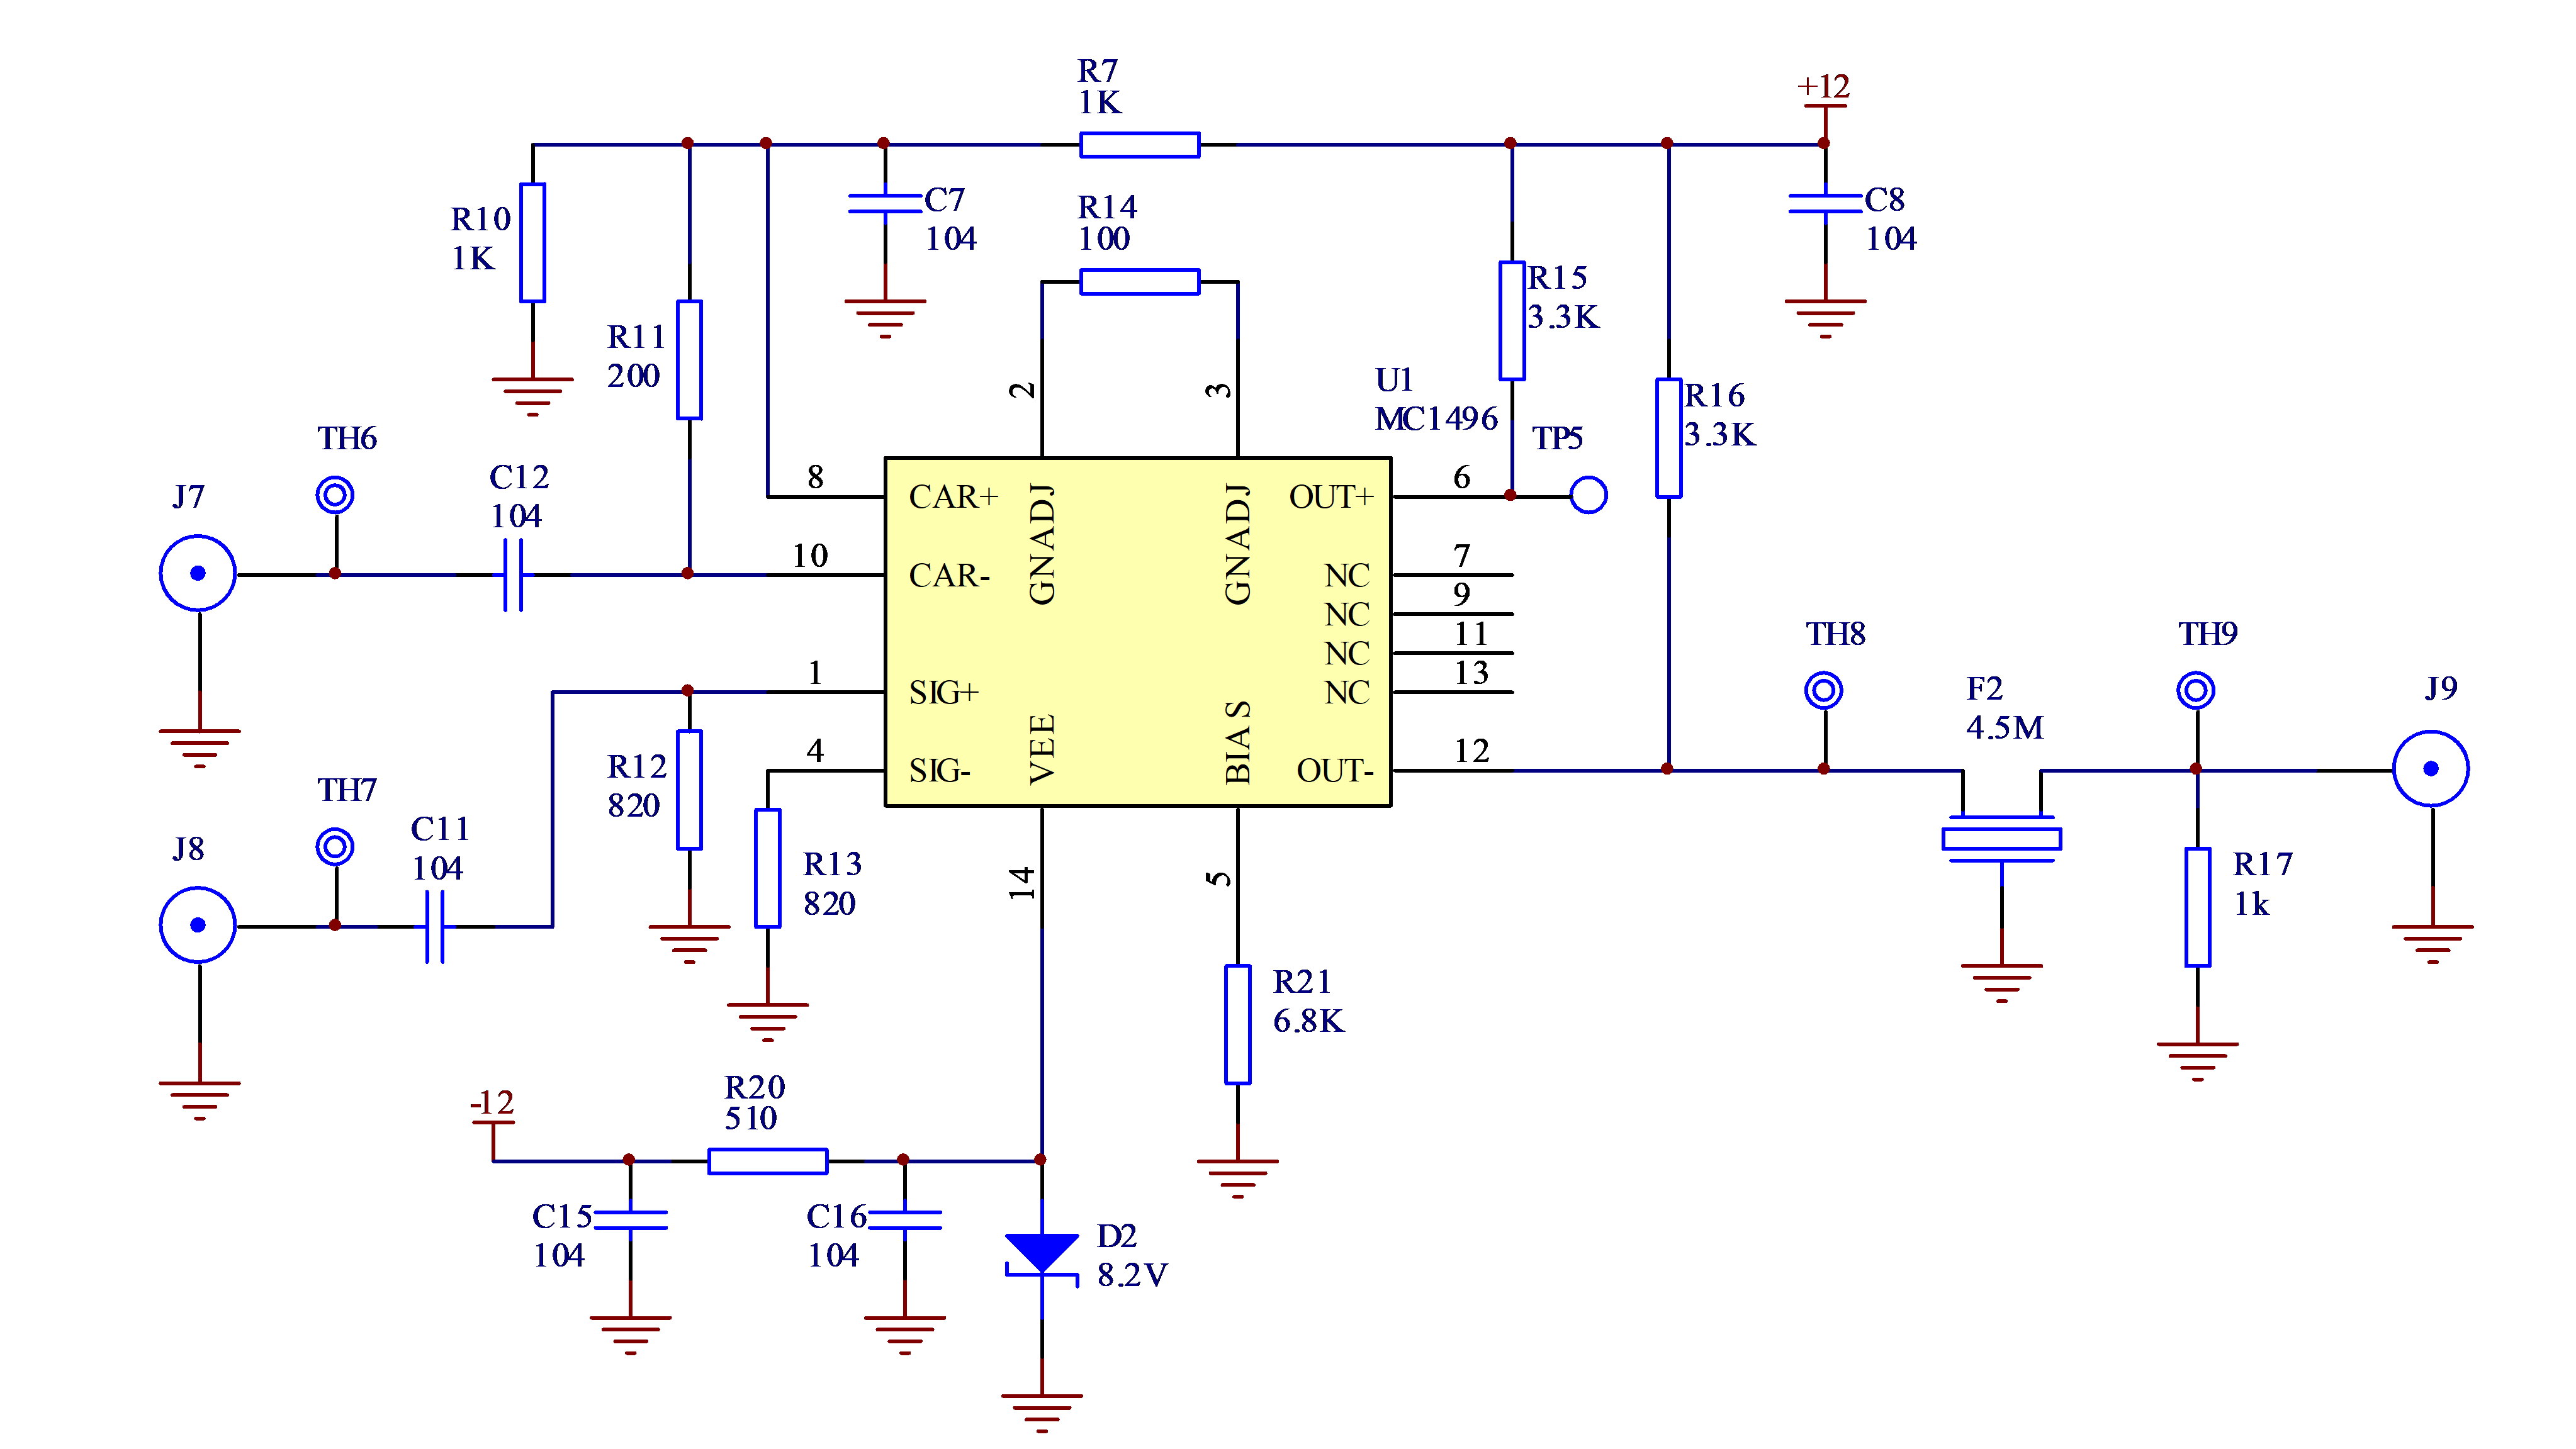
\includegraphics[width=\textwidth]{image002.png} 
  \caption{ MC1496构成的混频电路} 
  \label{img:cfhi} 
\end{figure}

\subsection{实验步骤}
\begin{enumerate}\addtolength{\itemsep}{-1.5ex}
\item  打开本实验单元的电源开关,观察对应的发光二极管是否点亮,熟悉电路各部分元件的作用。
\item  将(1号板提供)的晶体振荡频率$ f_S=4.19MHz$(幅度$V_{SP-P}=150mV$左右)的高频信号从相乘混频器的输入端J4口输入,用示波器观察输出端J5口处中频信号波形的变化,TH6处测试观察。
\item  用实验箱的信号源做本振信号,将频率$f_L =8.7MHz$(幅度$V_{LP-P}=300mV$左右)的本振信号从J3口处输入(本振输入处),在相乘混频器的输出端J5口处观察输出中频信号波形,TH6处测试观察。

\item  用示波器观察TH7和TH6处波形。
\item  改变高频信号电压幅度,用示波器观测,记录输出中频电压Vi的幅值,并填入表\ref{tab:aj}。
\begin{table}[htbp]
\centering
\caption{高频信号电压幅度与中频电压幅值关系}
\label{tab:aj}
\begin{tabular}{|c|c|c|c|c|}
\hline
$V_{SP-P}(mv)$ & 150 & 200 & 300 & 364 \\ \hline
$V_{iP-P}(mv)$ & 378 & 456 & 508 & 520 \\ \hline
\end{tabular}
\end{table}
\item  改变本振信号电压幅度,用示波器观测,记录输出中频电压Vi的幅值,并填入表\ref{tab:ajk}。
\begin{table}[htbp]
\centering
\caption{本振信号电压幅度与中频电压幅值关系}
\label{tab:ajk}
\begin{tabular}{|c|c|c|c|c|c|}
\hline
$V_{LP-P}(mv)$ & 150 & 300 & 400 & 500 & 600 \\ \hline
$V_{iP-P}(mv)$ & 216 & 366 & 452 & 508 & 528 \\ \hline
\end{tabular}
\end{table}
    \end{enumerate}
\subsection{实验仪器}
\begin{tabular}{clcc}
1.&	高频实验箱                &&        1台 \\
2.&	双踪示波器           &&             1台\\
\end{tabular}
\subsection{实验结果}
\begin{enumerate}\addtolength{\itemsep}{-1.5ex}
\item 对于表\ref{tab:aj},由示波器测得的信号源本振信号的输入波形见图\ref{img:bzbx},其对应的波形情况见表\ref{tab:ajk2}。
       \begin{figure}[ht]
  \centering
  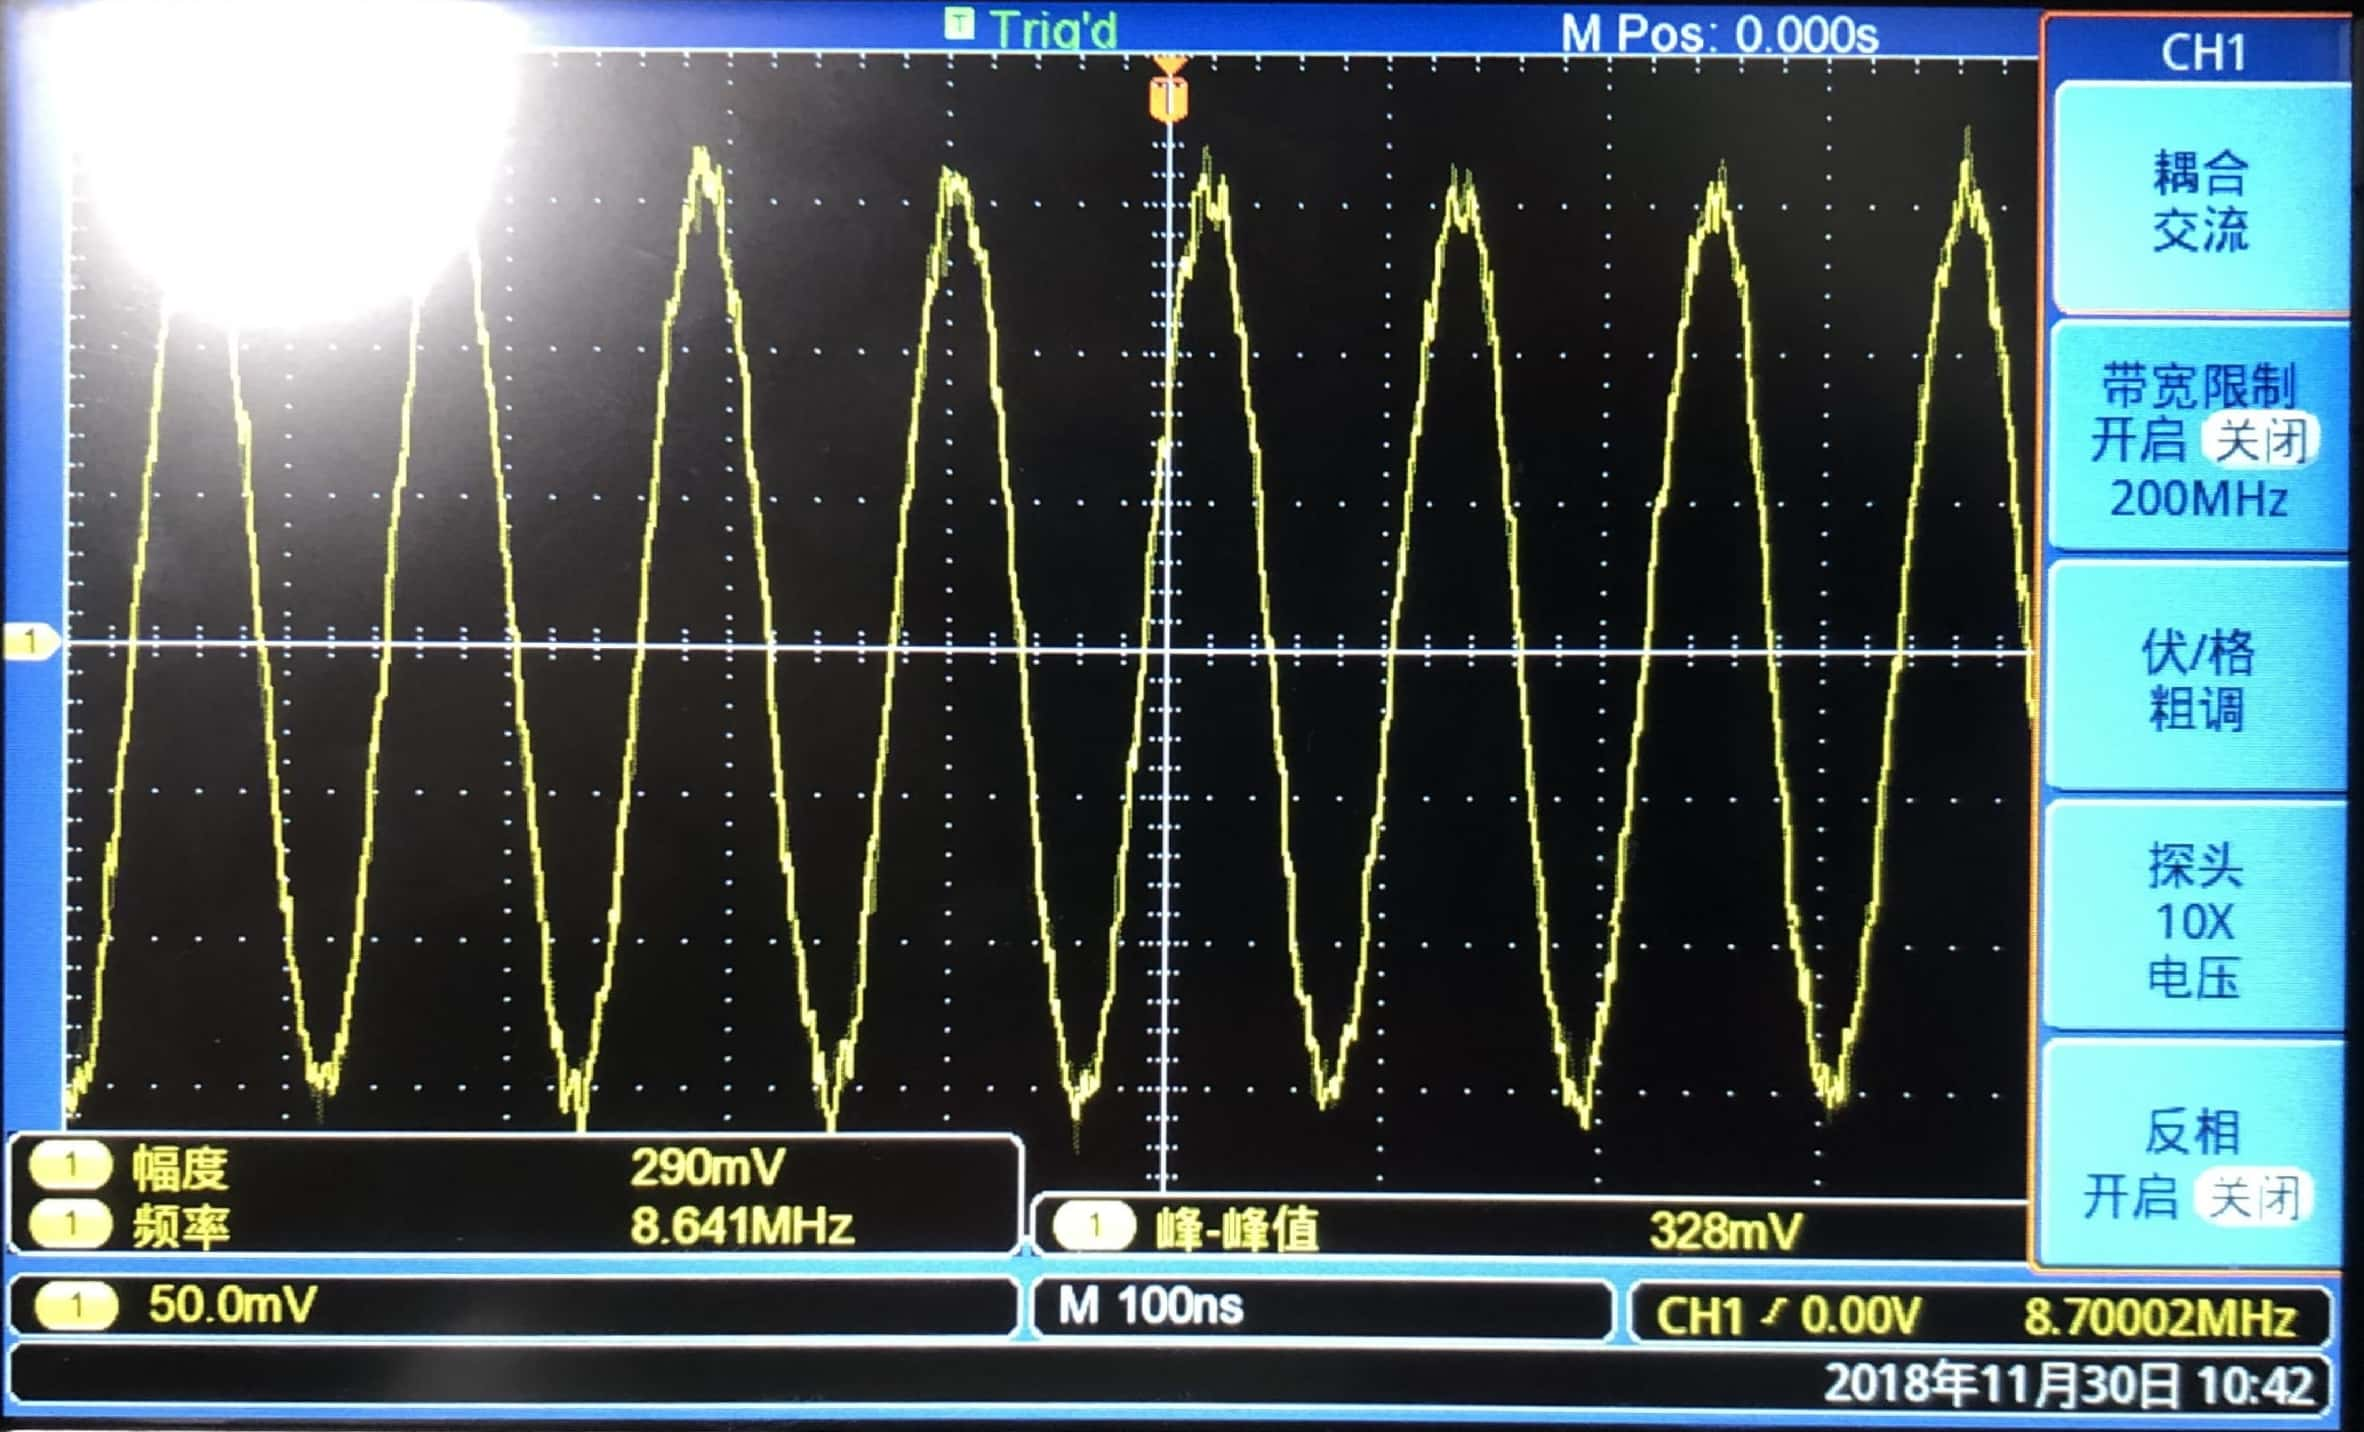
\includegraphics[width=.4\textwidth]{gaopin3/gaopin311.jpg} 
  \caption{ 信号源本振信号波形} 
  \label{img:bzbx} 
\end{figure}

\begin{table}[htbp]
\centering
\caption{高频信号电压幅度与中频电压幅值关系波形情况}
\label{tab:ajk2}
\begin{tabular}{|c|c|c|c|}
\hline
$V_{SP-P}(mv)$ & 波形 & $V_{iP-P}(mv)$ & 波形 \\\hline
150            &   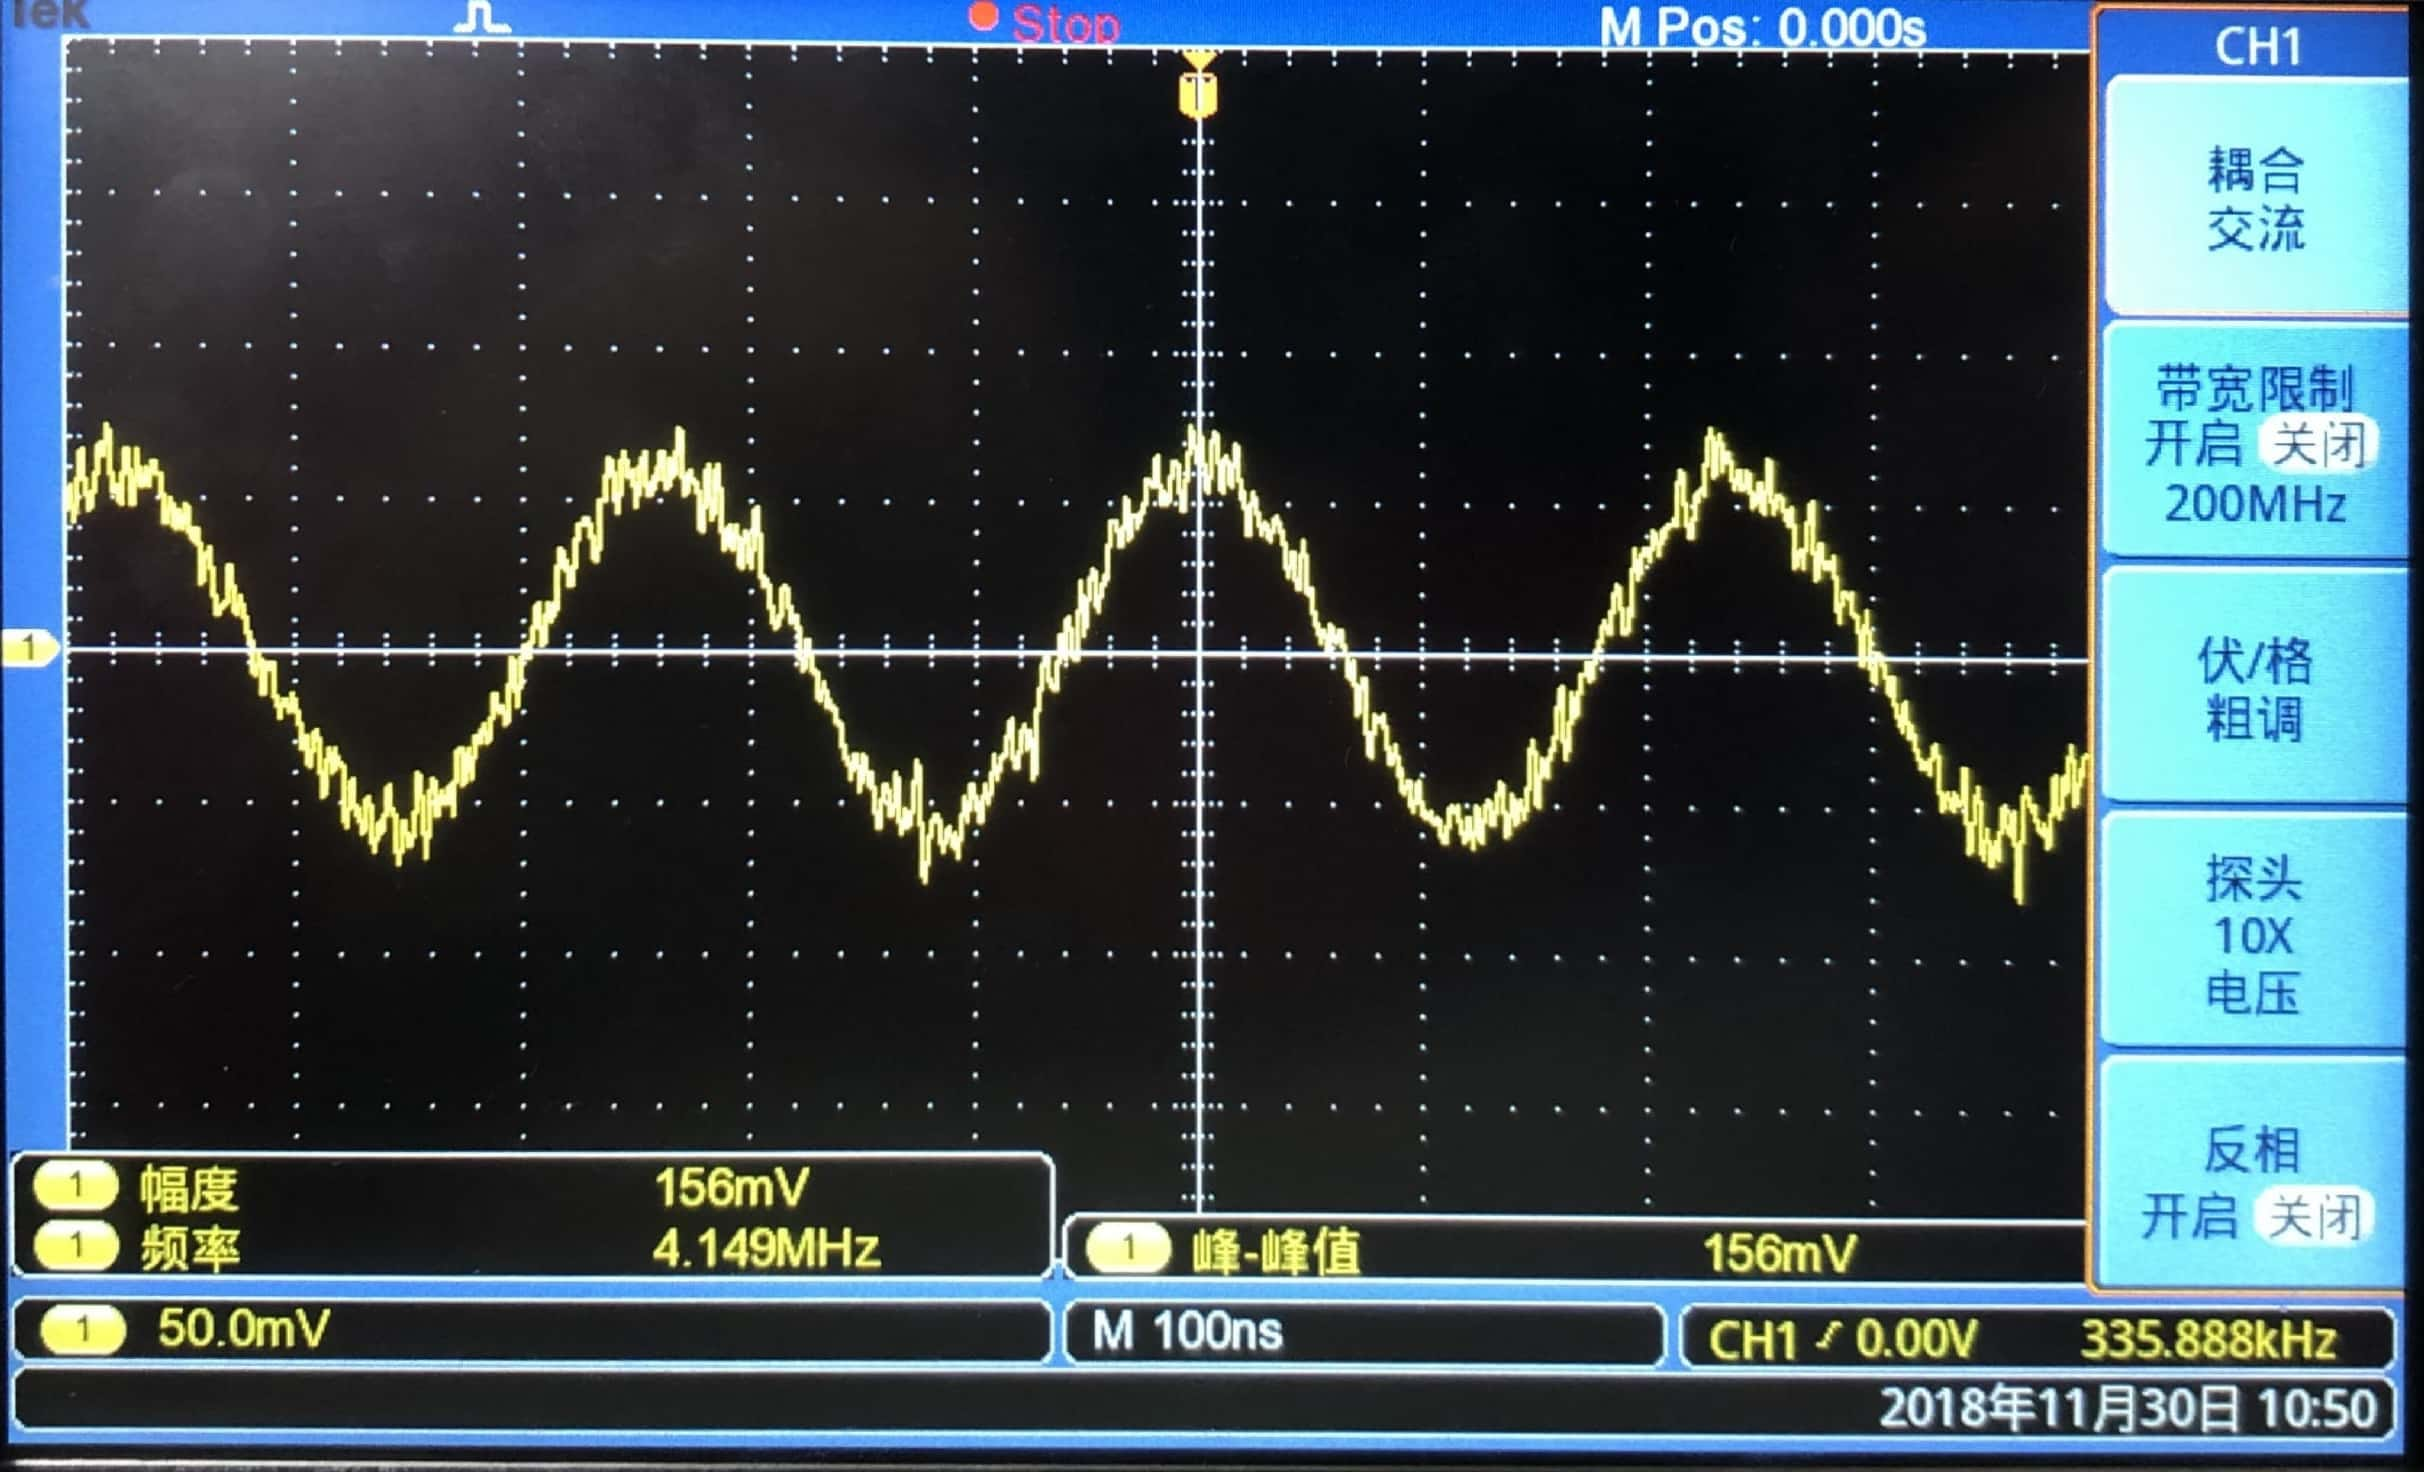
\includegraphics[width=0.35\textwidth]{gaopin3/gaopin310.jpg} & 378            &    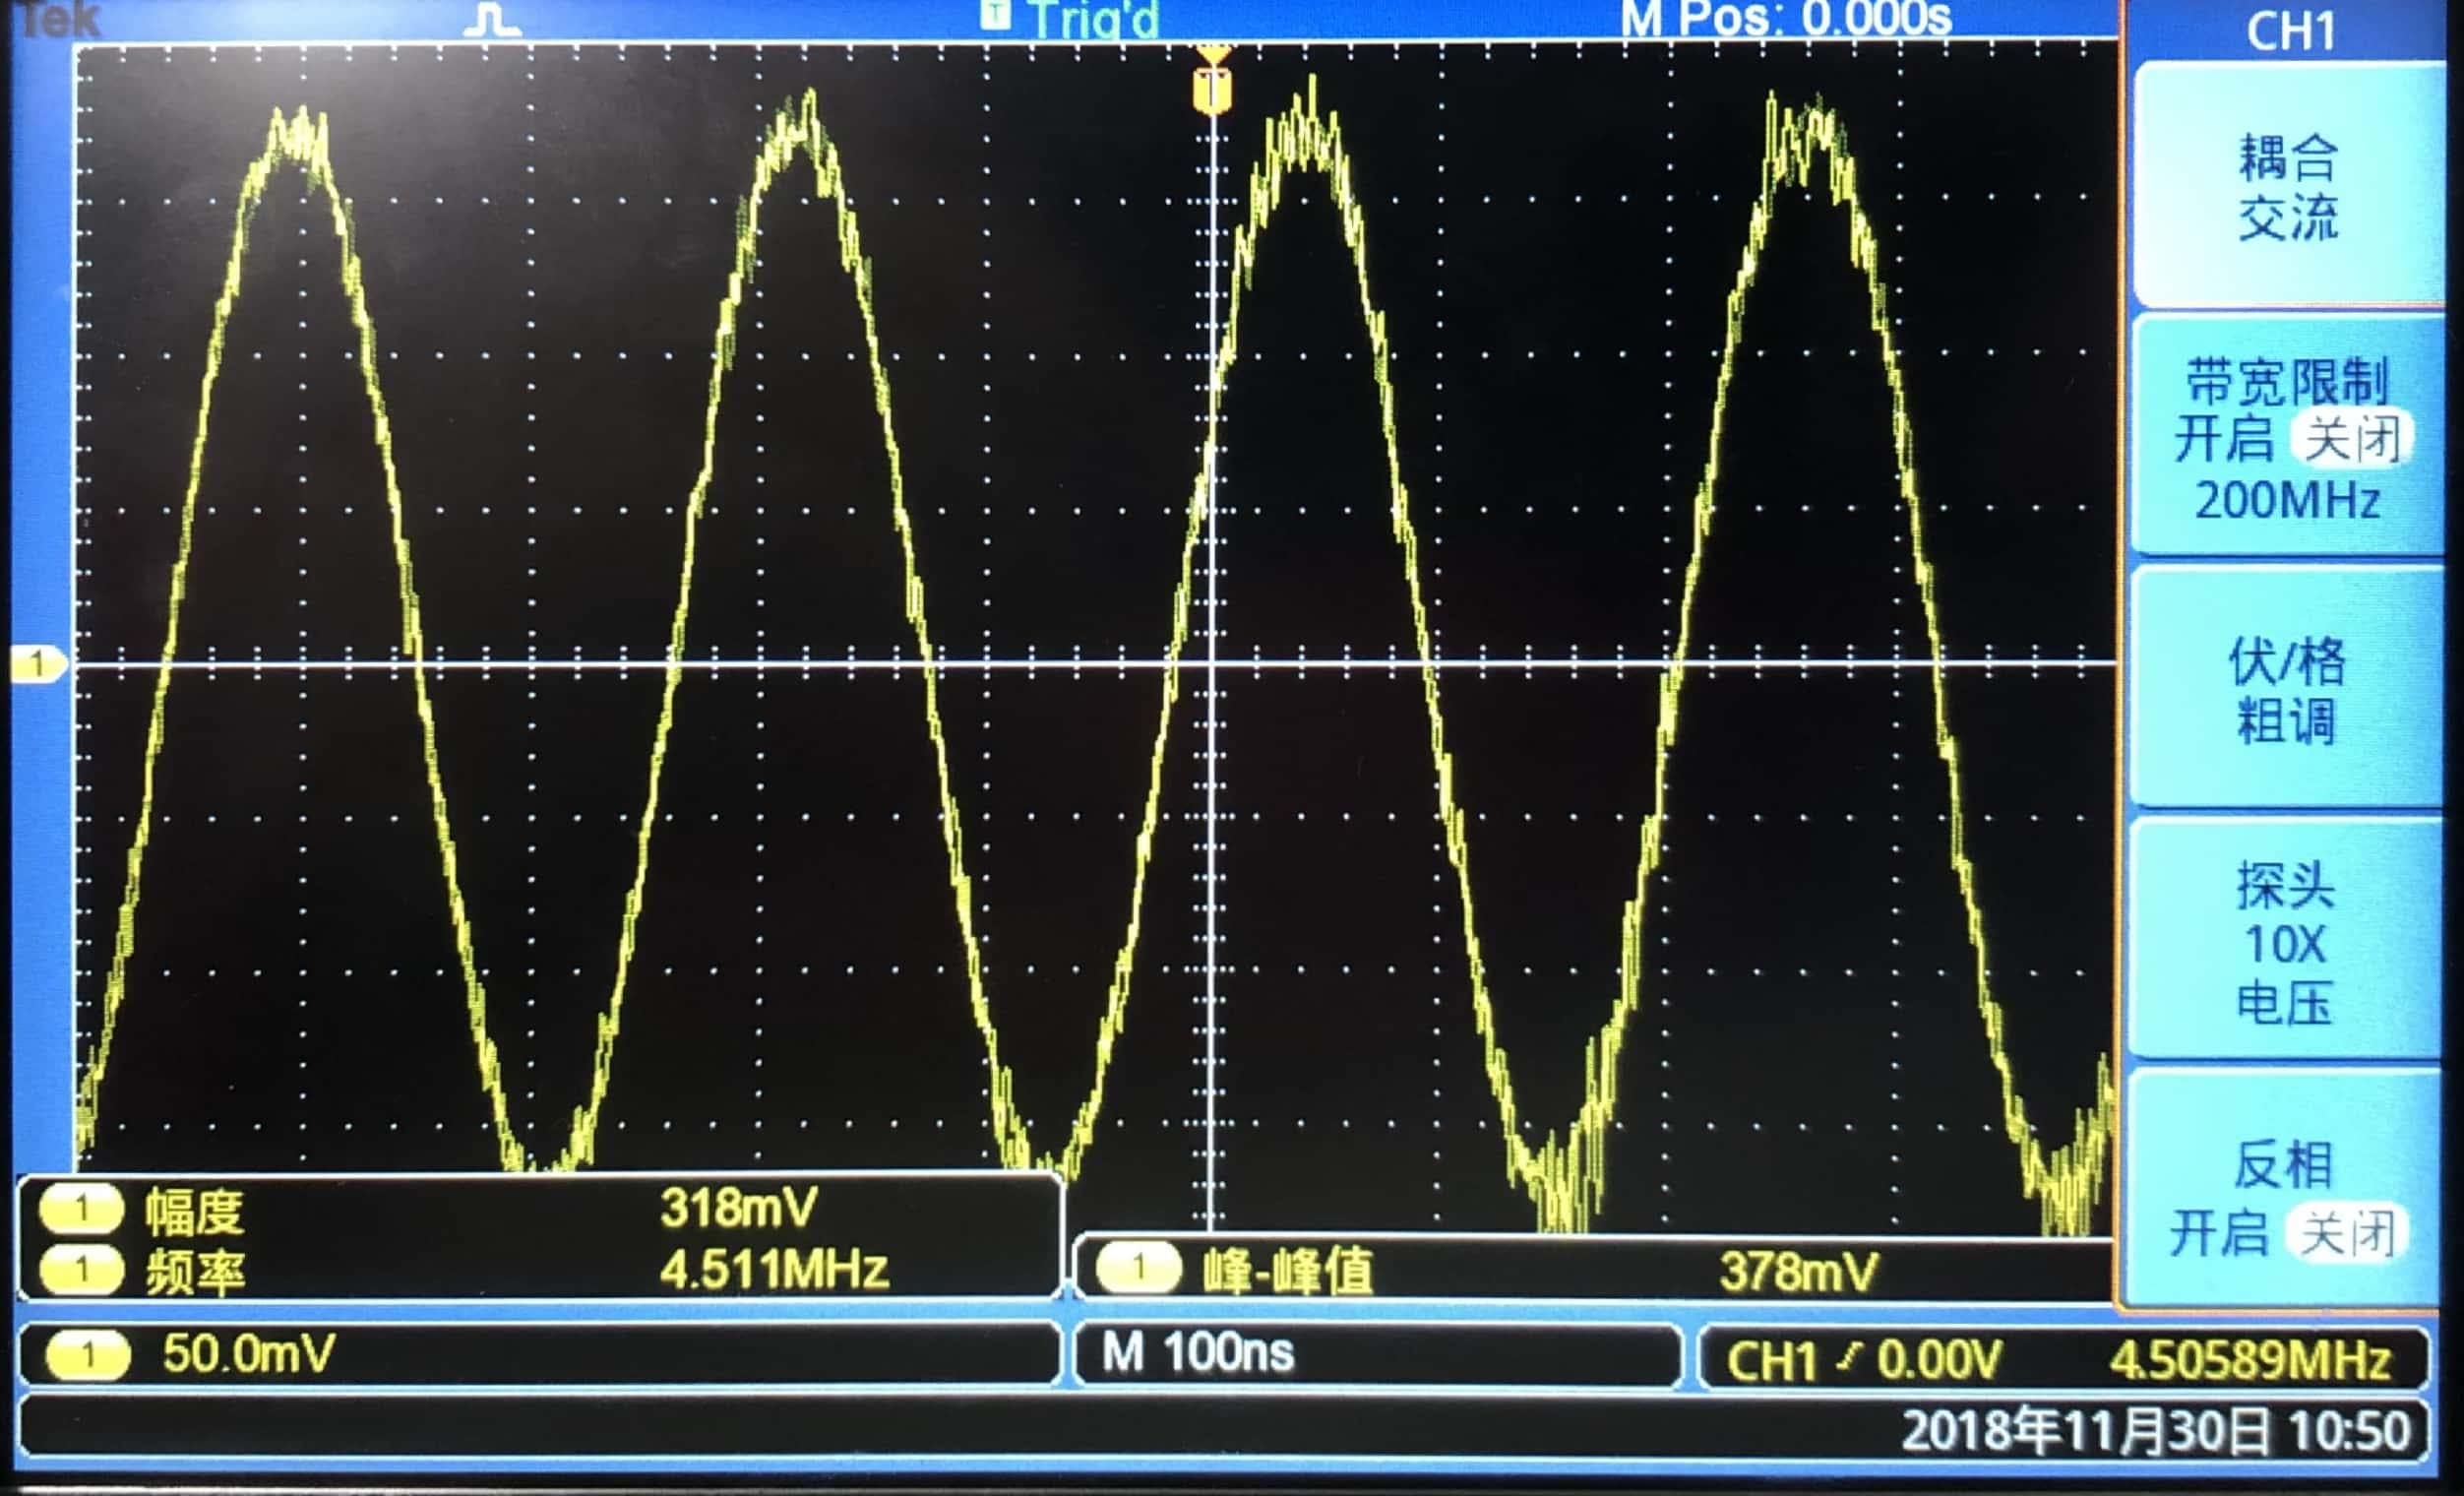
\includegraphics[width=0.35\textwidth]{gaopin3/gaopin318.jpg}\\\hline
200            & 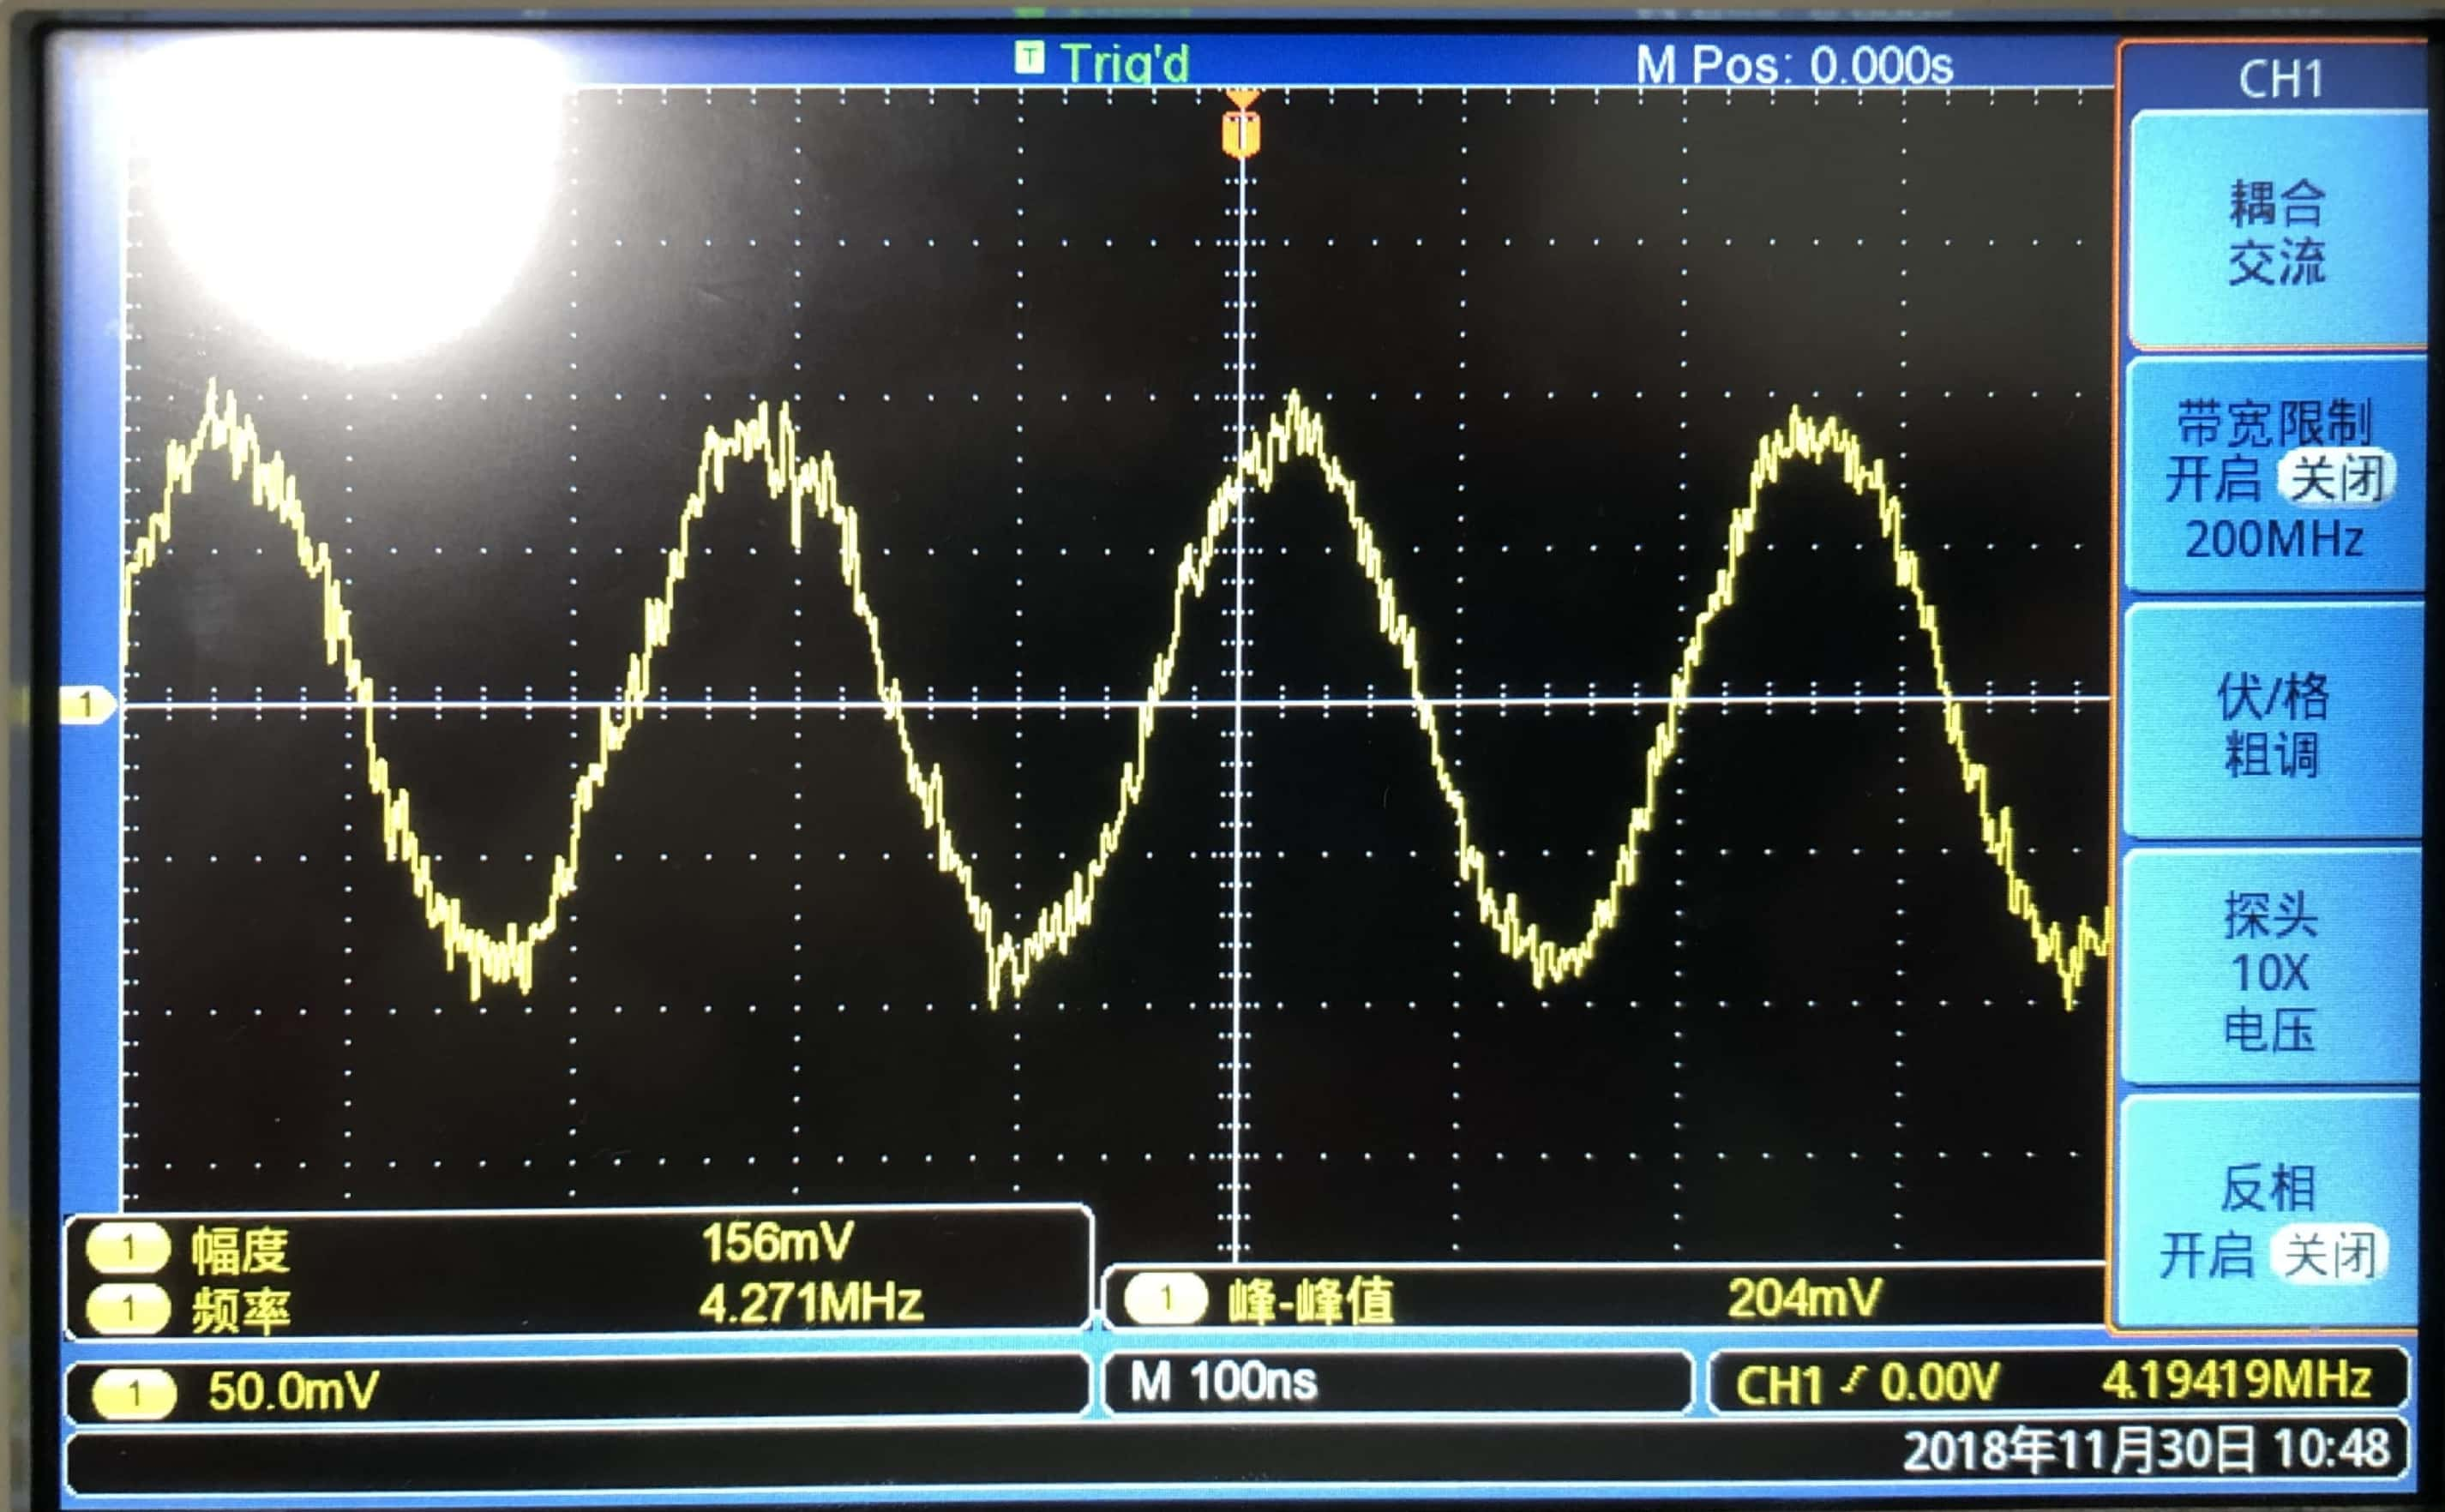
\includegraphics[width=0.35\textwidth]{gaopin3/gaopin315.jpg}   & 456            & 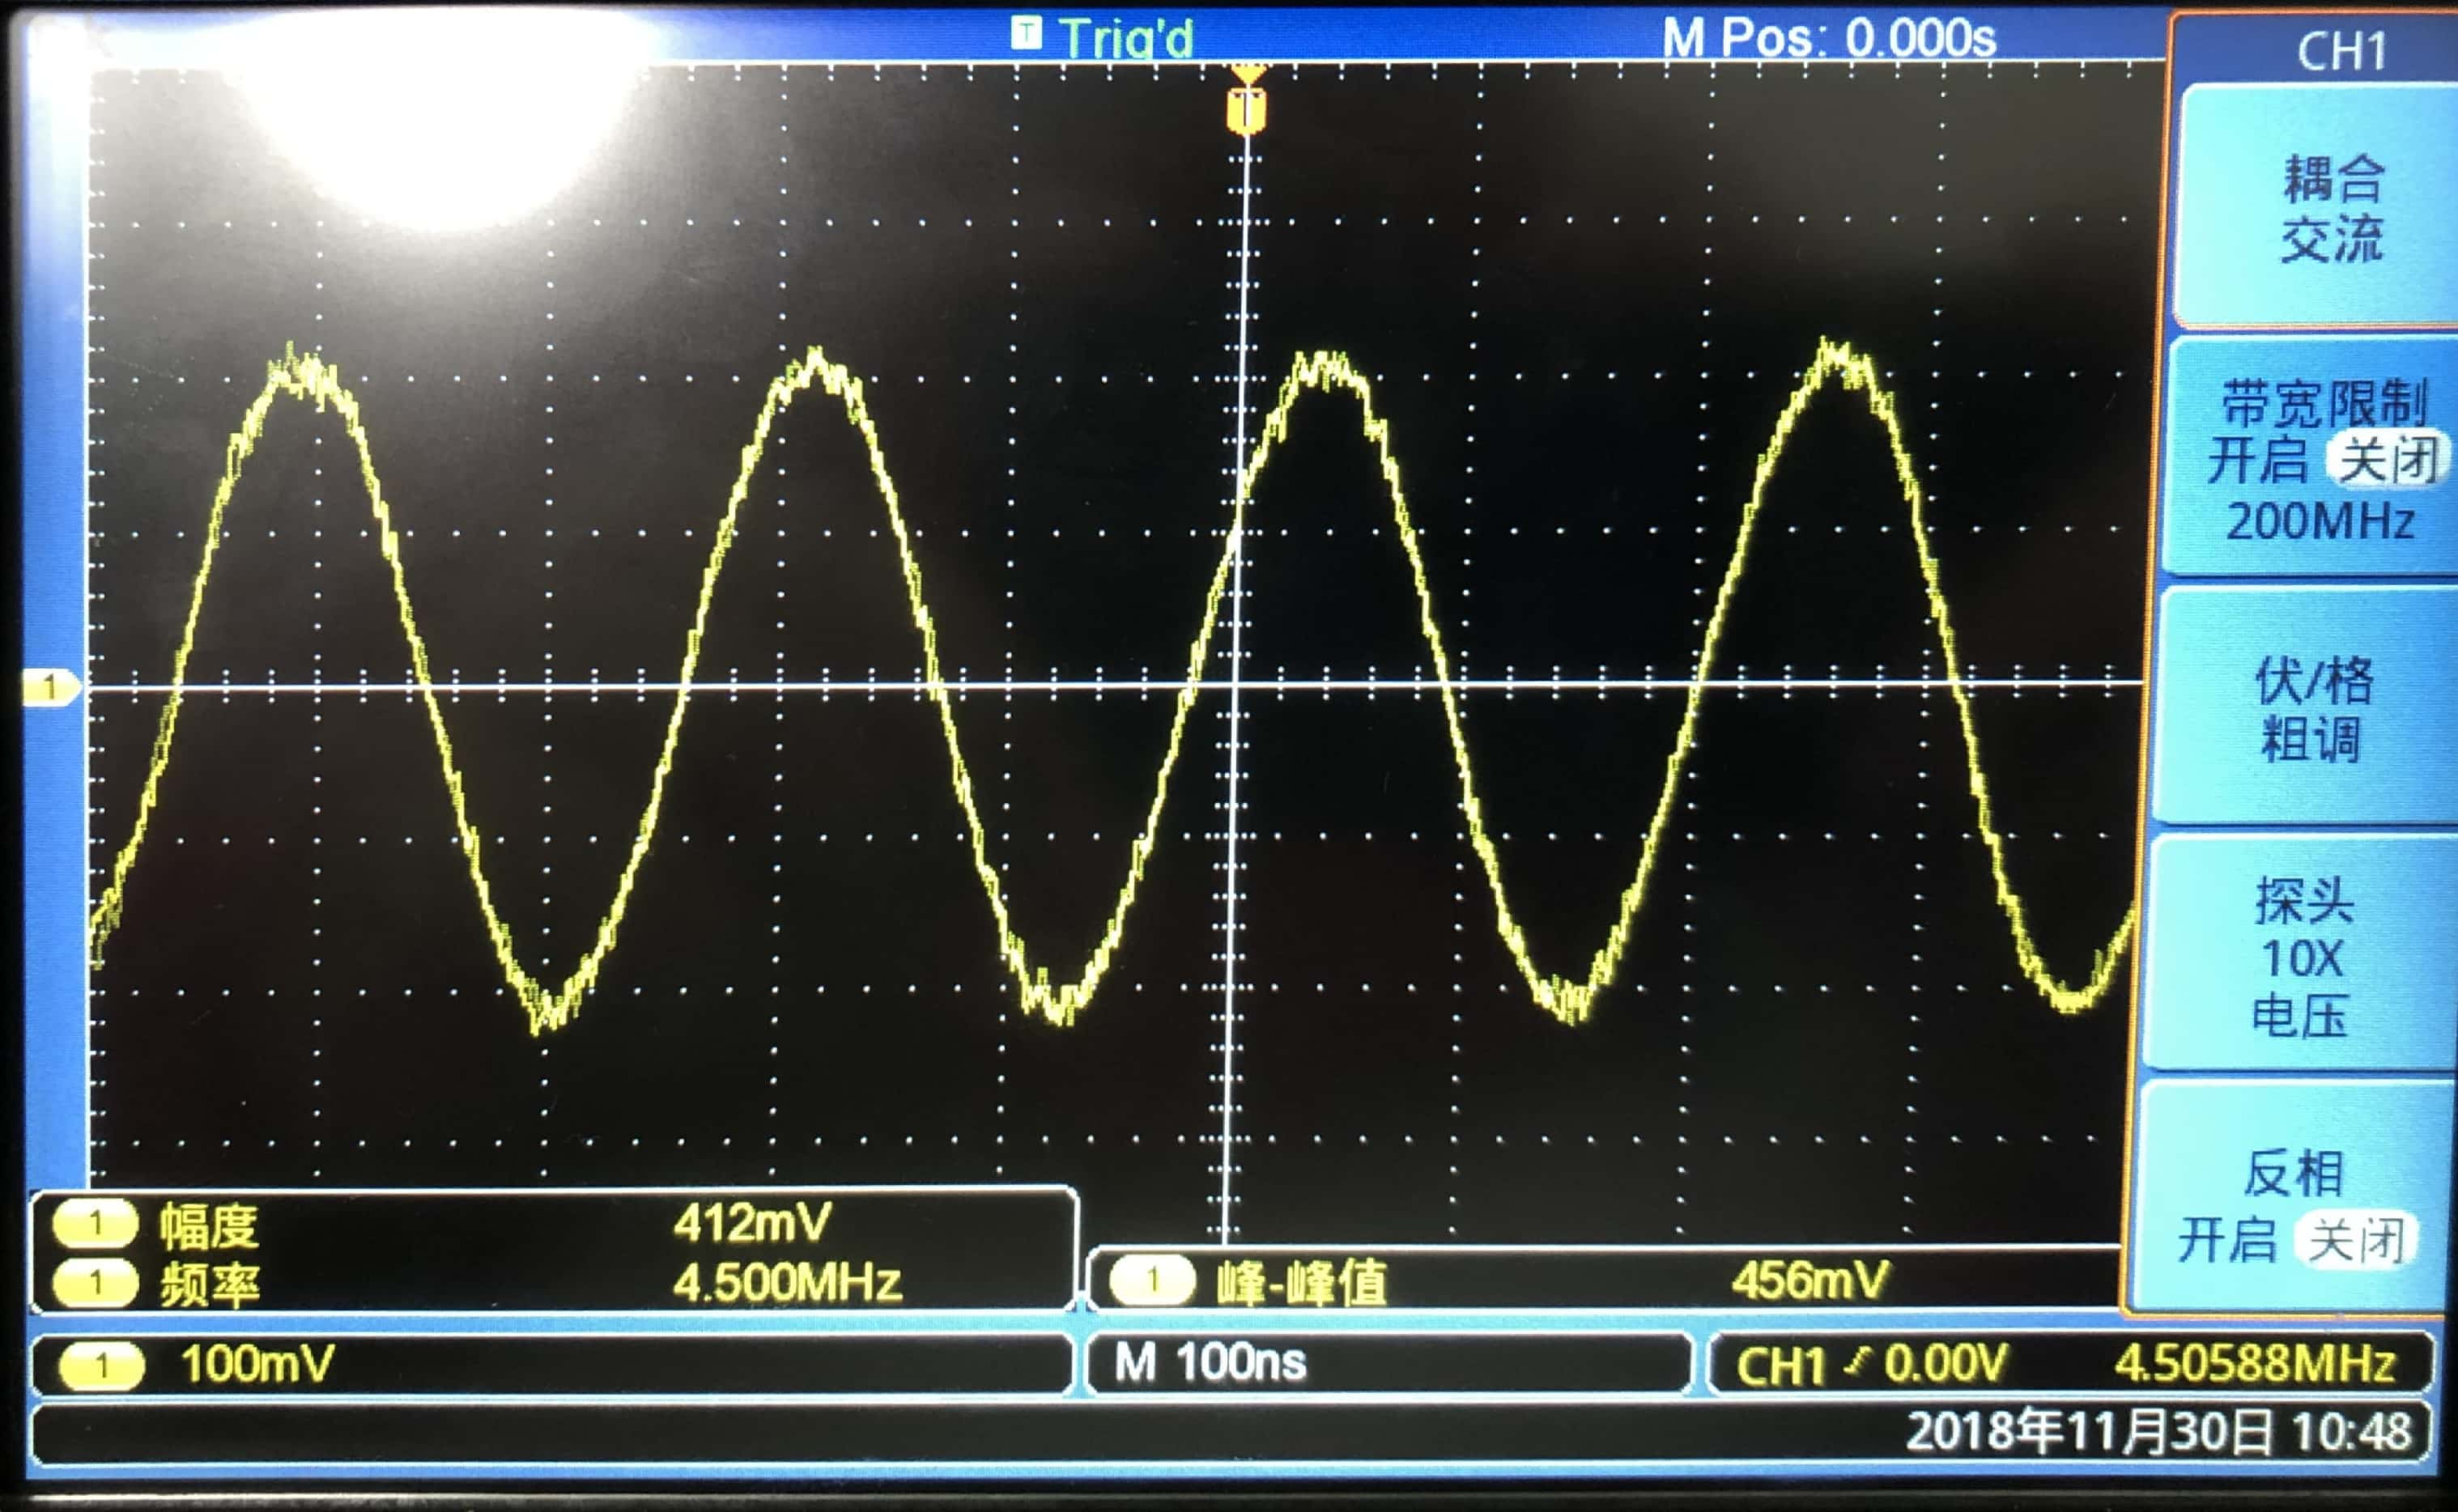
\includegraphics[width=0.35\textwidth]{gaopin3/gaopin317.jpg} \\\hline
300            &  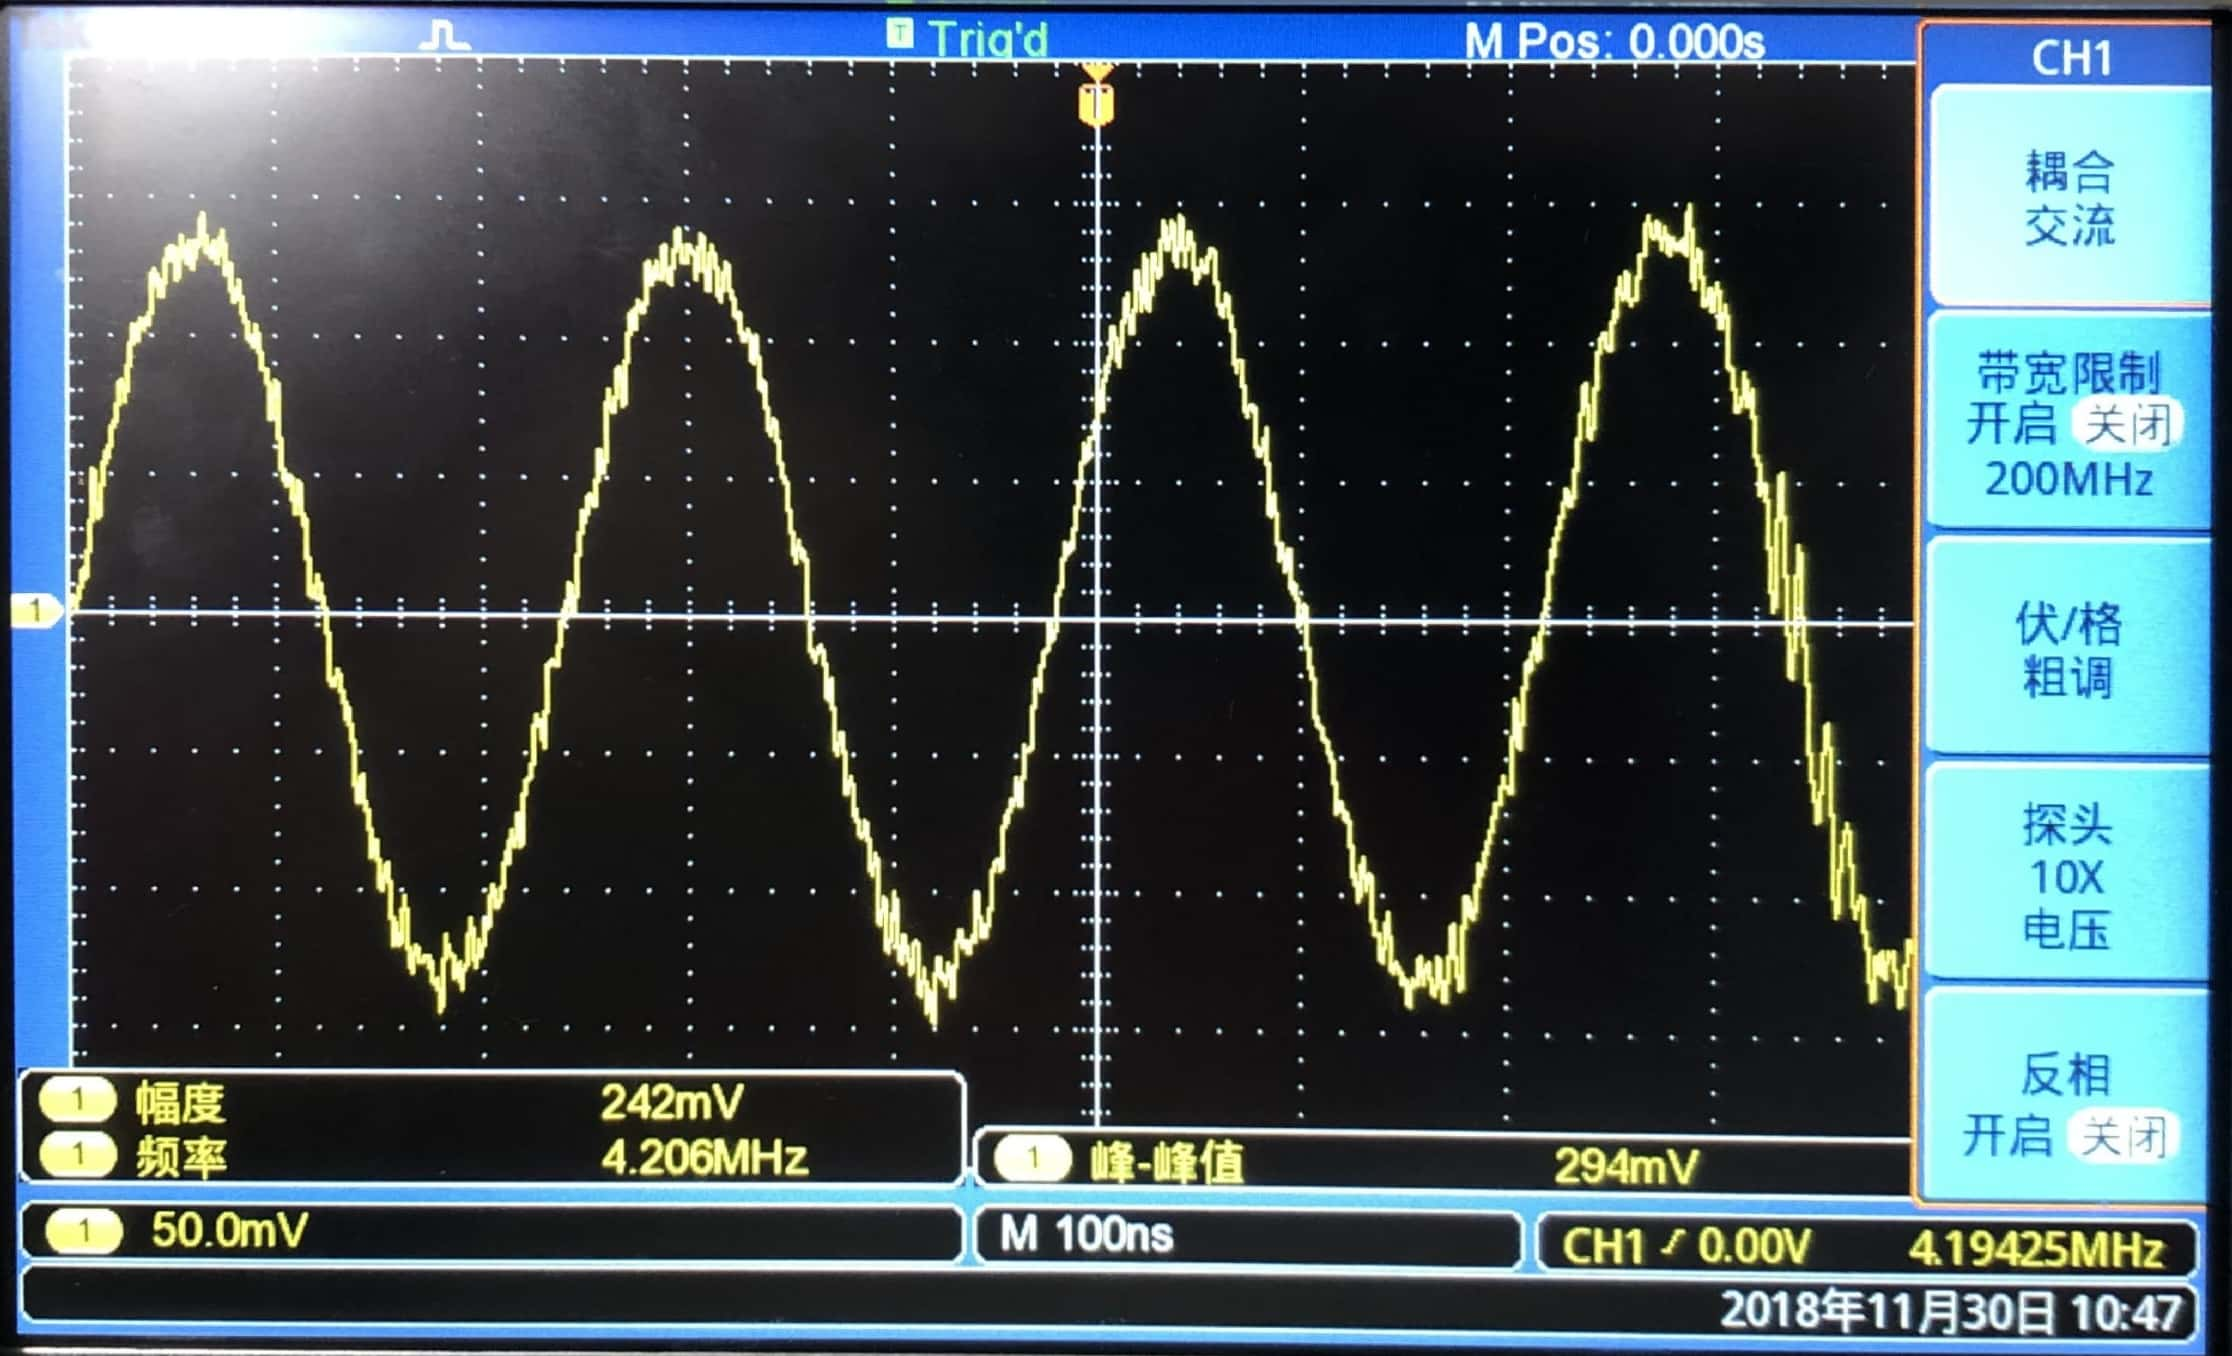
\includegraphics[width=0.35\textwidth]{gaopin3/gaopin313.jpg}  & 508            & 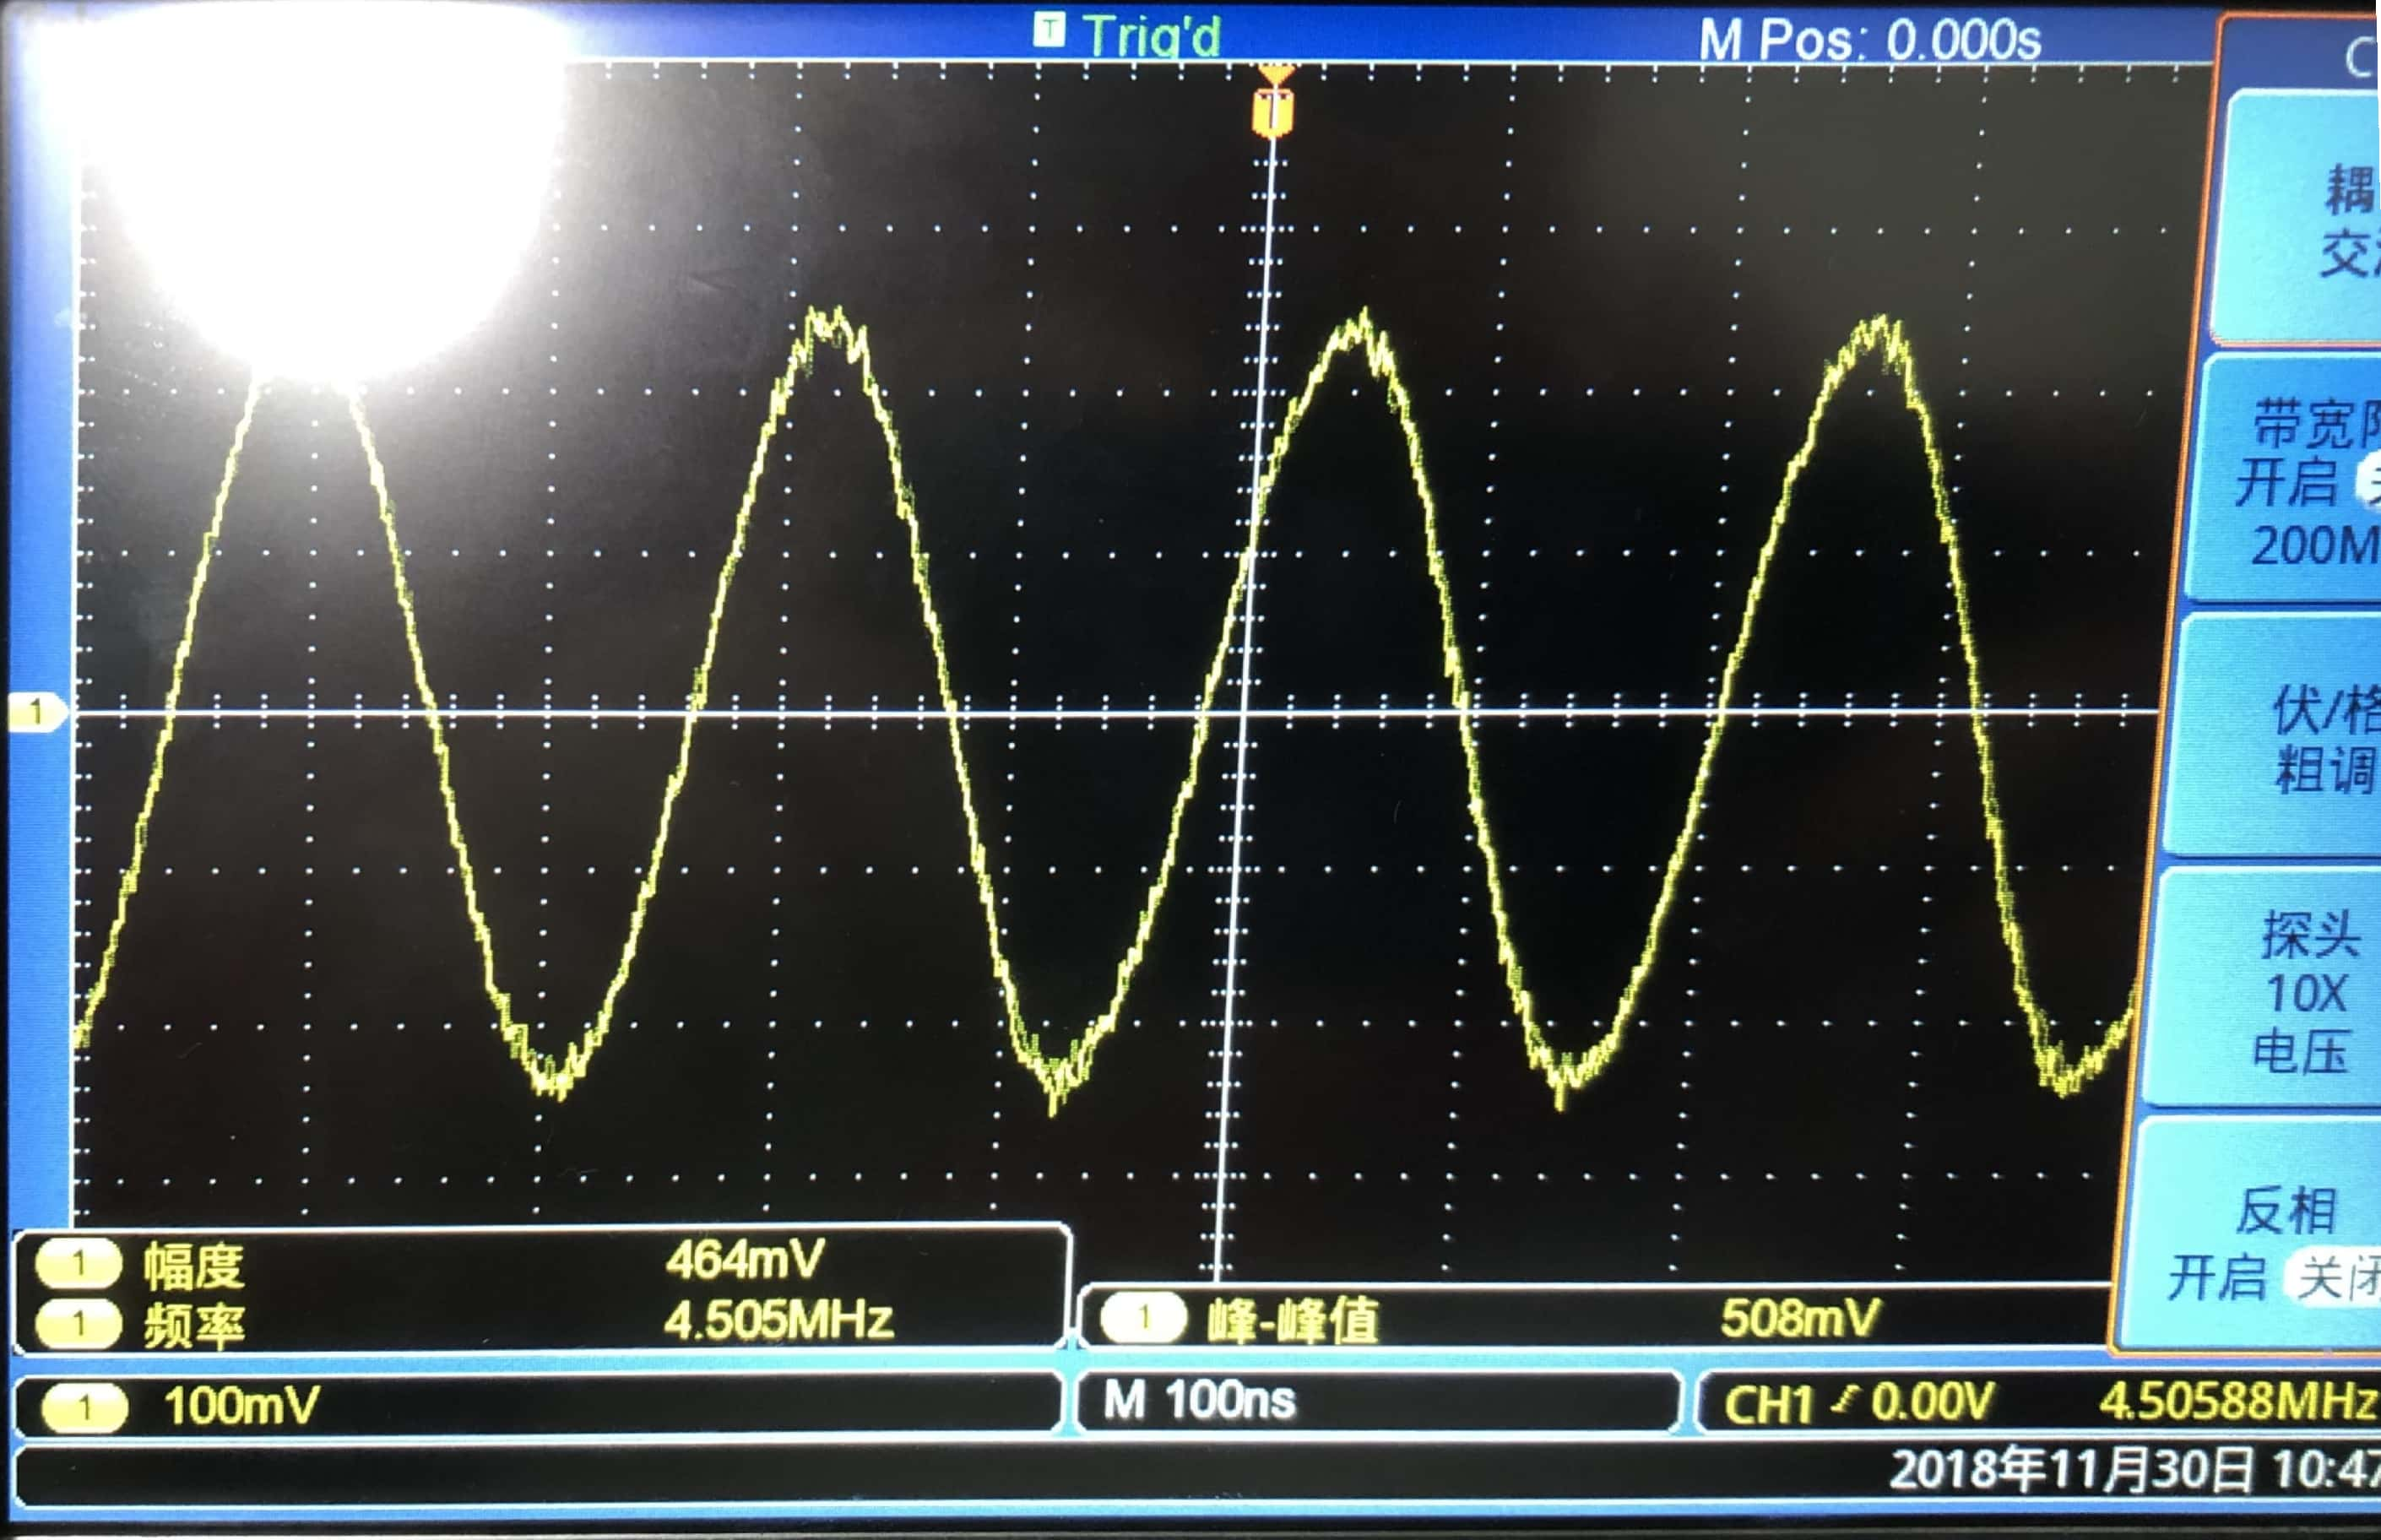
\includegraphics[width=0.35\textwidth]{gaopin3/gaopin309.jpg}  \\\hline
364            &  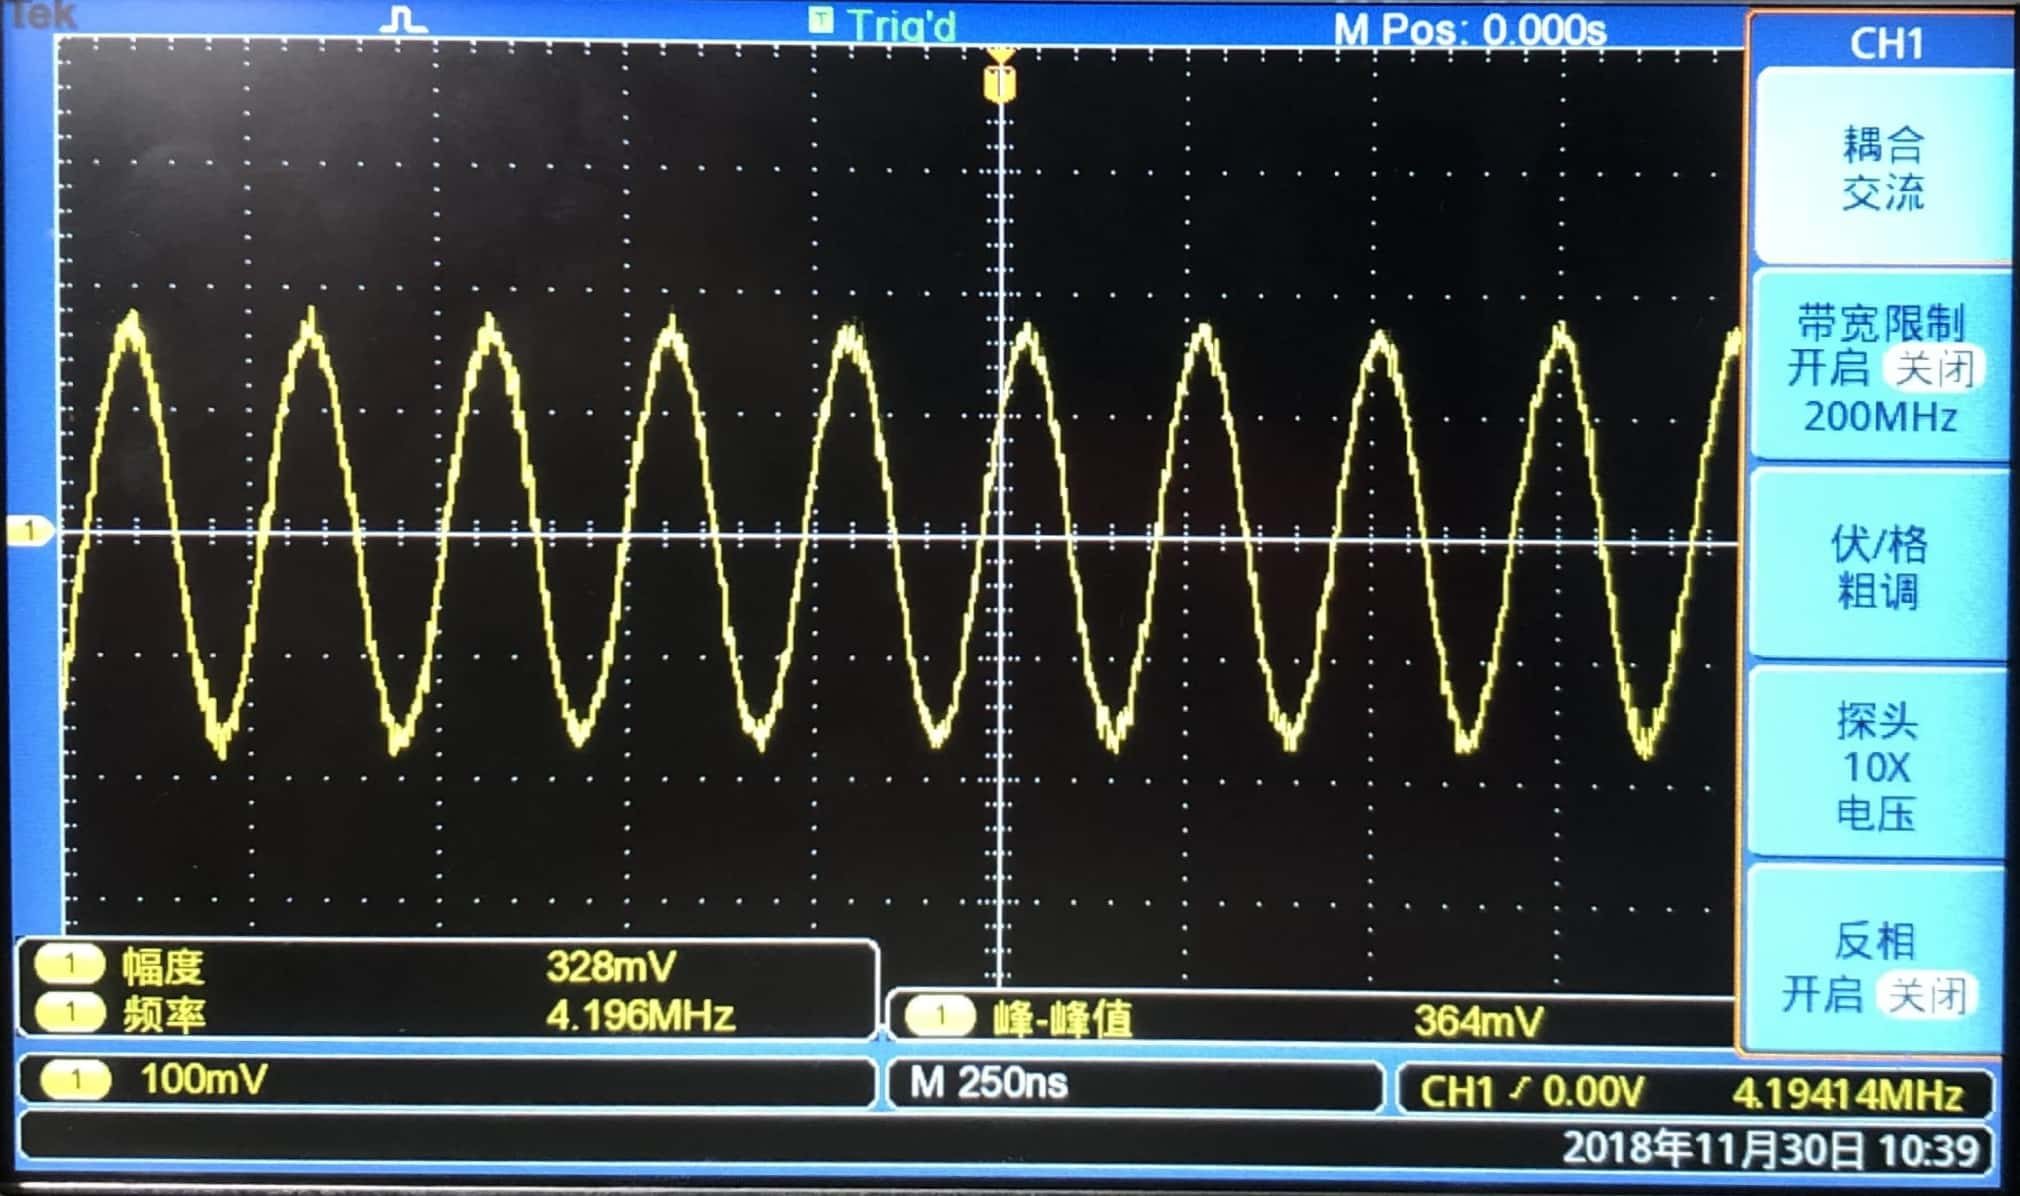
\includegraphics[width=0.35\textwidth]{gaopin3/gaopin316.jpg}  & 520            &    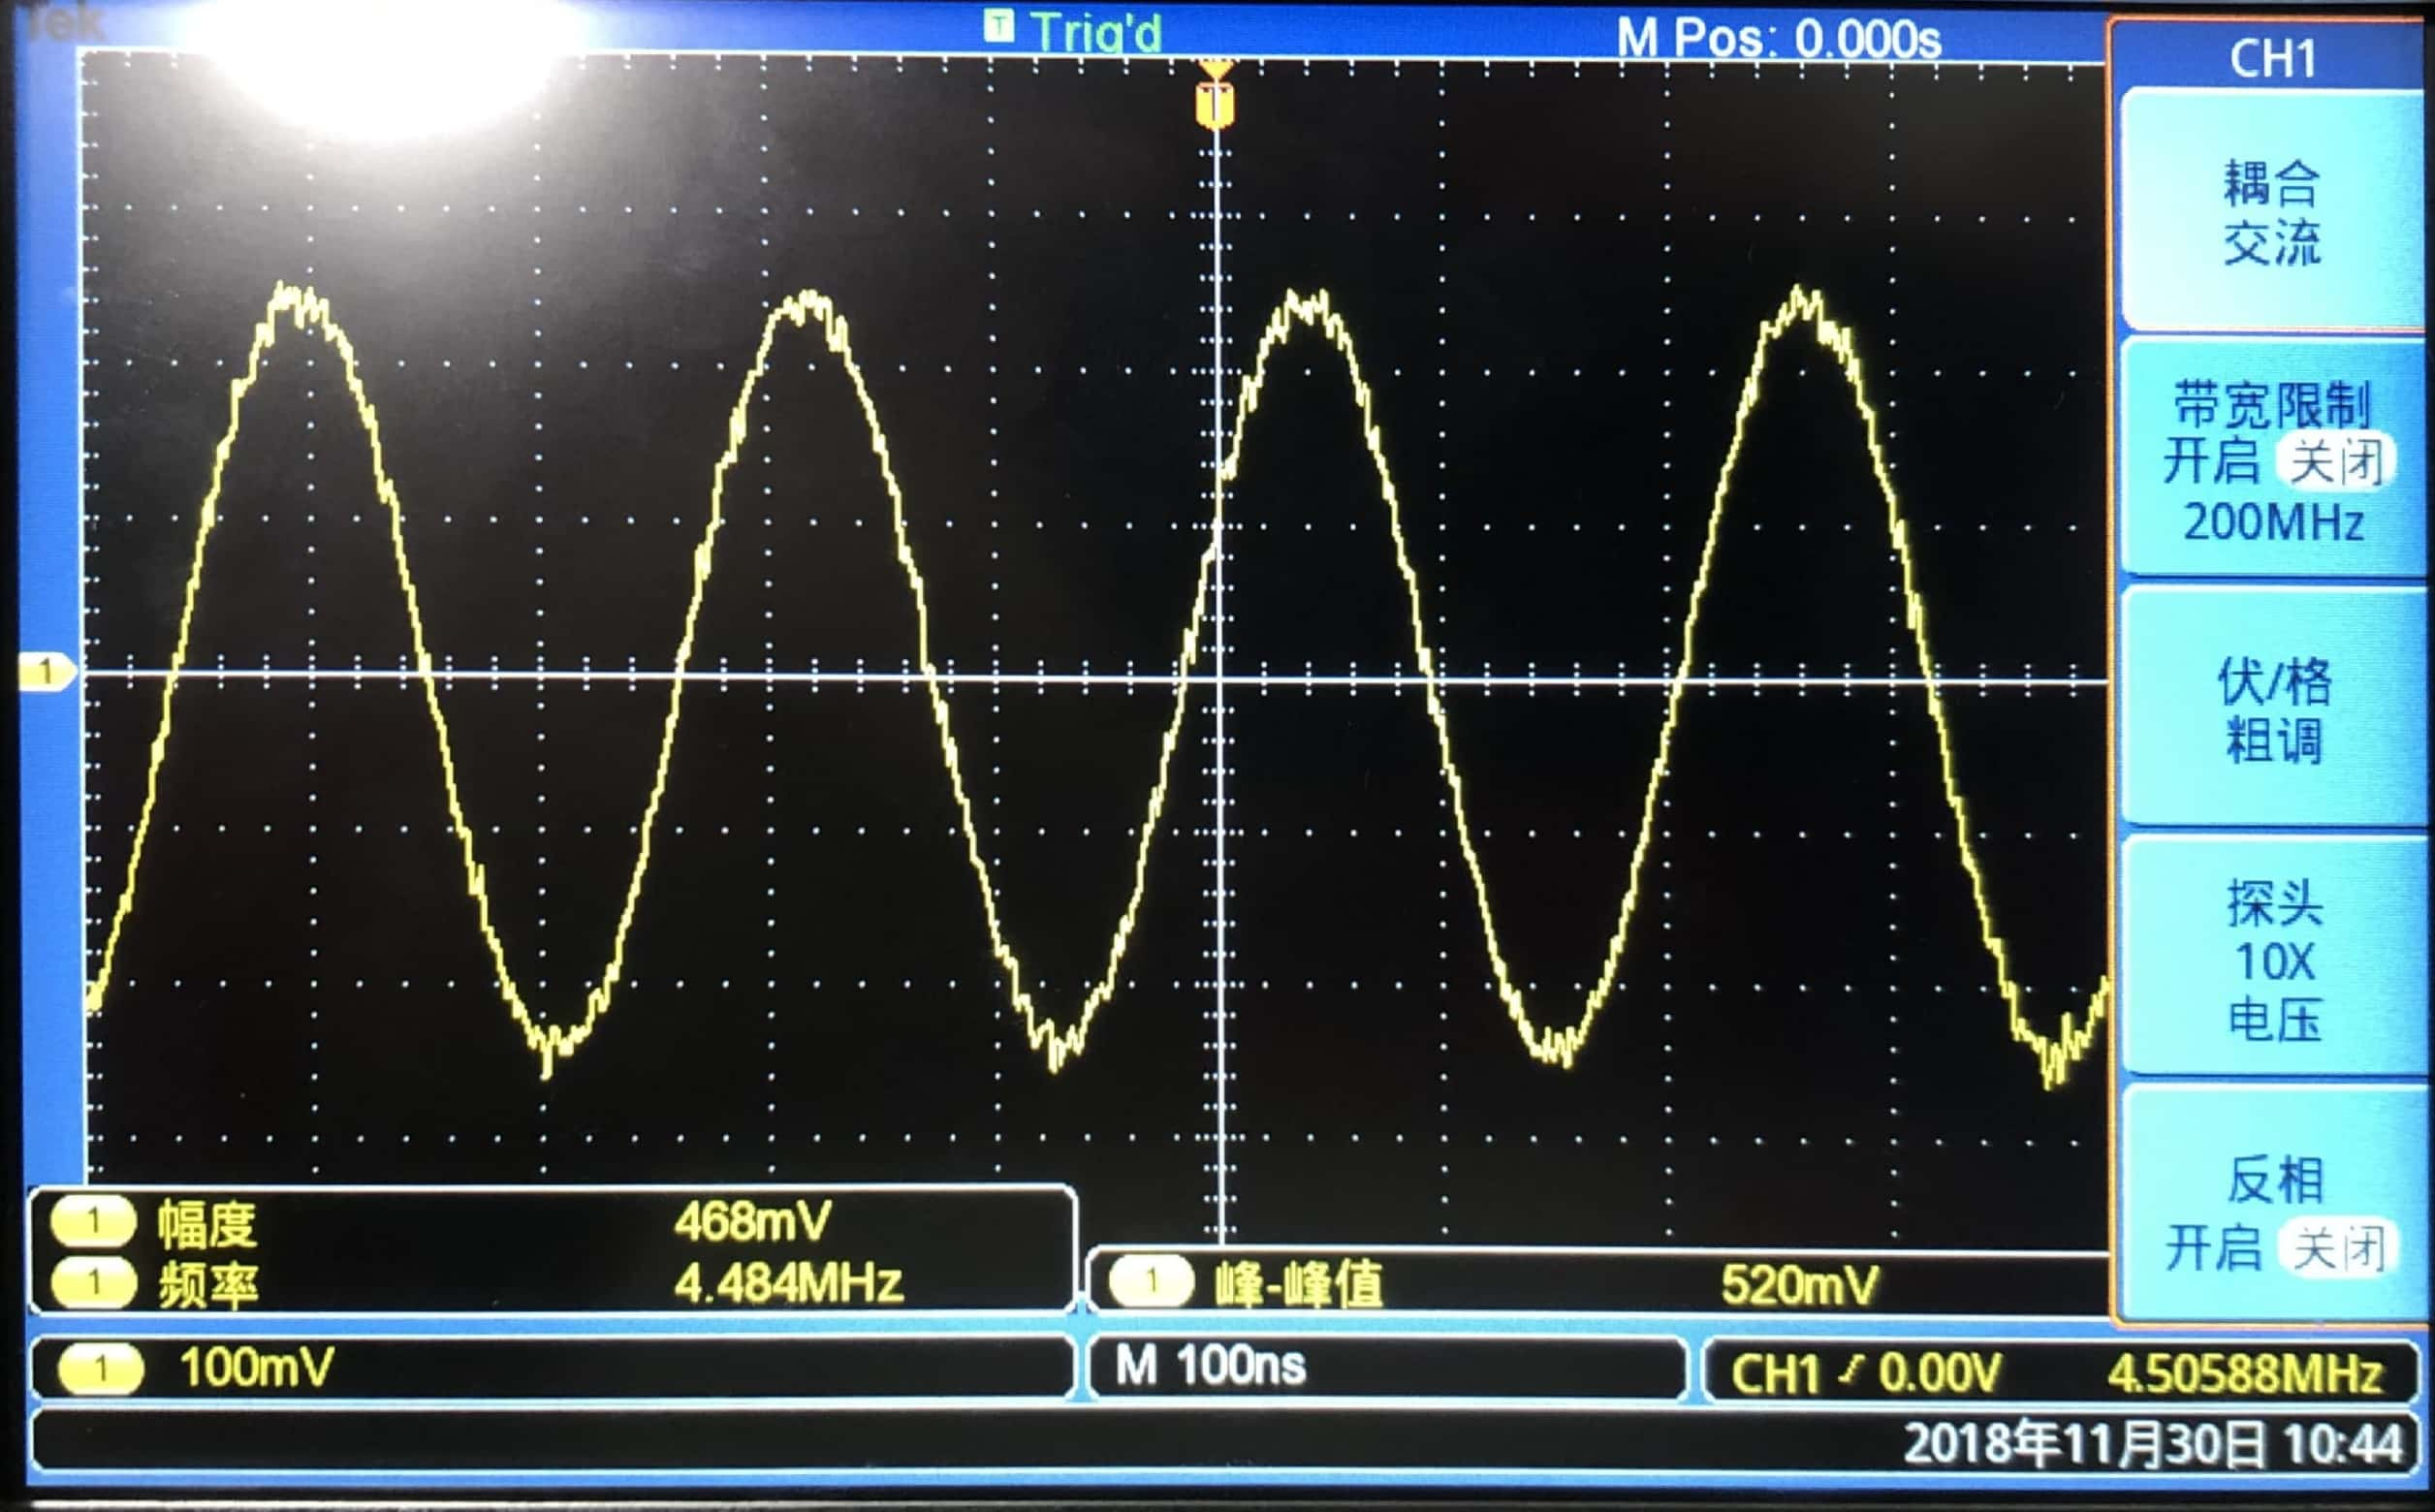
\includegraphics[width=0.35\textwidth]{gaopin3/gaopin314.jpg} \\\hline
\end{tabular}
\end{table}

\begin{table}[htbp]
\centering
\caption{本振信号电压幅度与中频电压幅值关系波形情况}
\label{tab:ajk3}
\begin{tabular}{|c|c|c|c|}
\hline
$V_{LP-P}(mv)$ & 波形 & $V_{iP-P}(mv)$ & 波形 \\ \hline
150            &   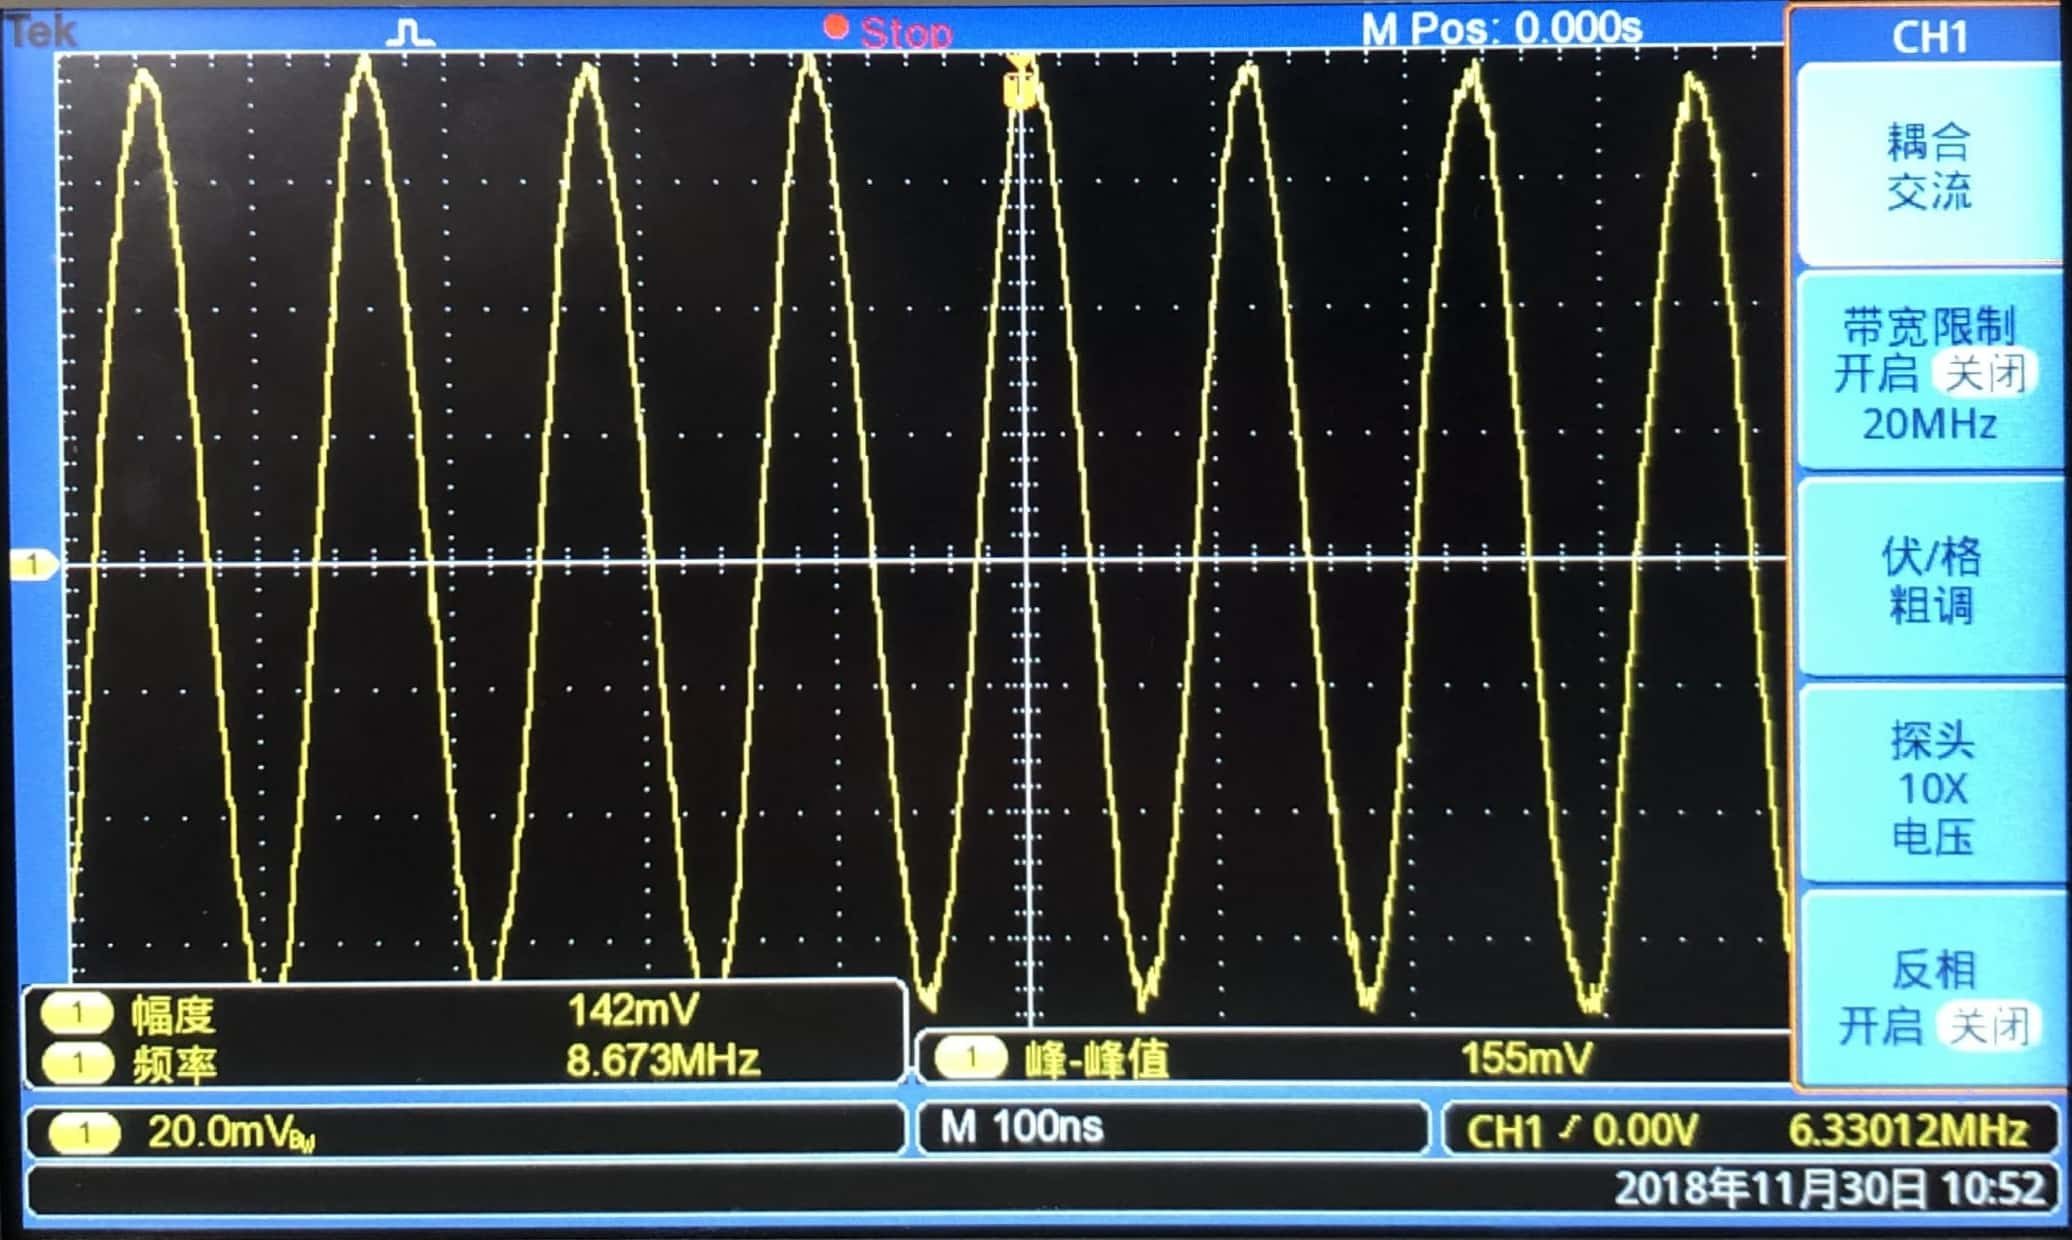
\includegraphics[width=0.35\textwidth]{gaopin3/gaopin319.jpg}   & 216            & 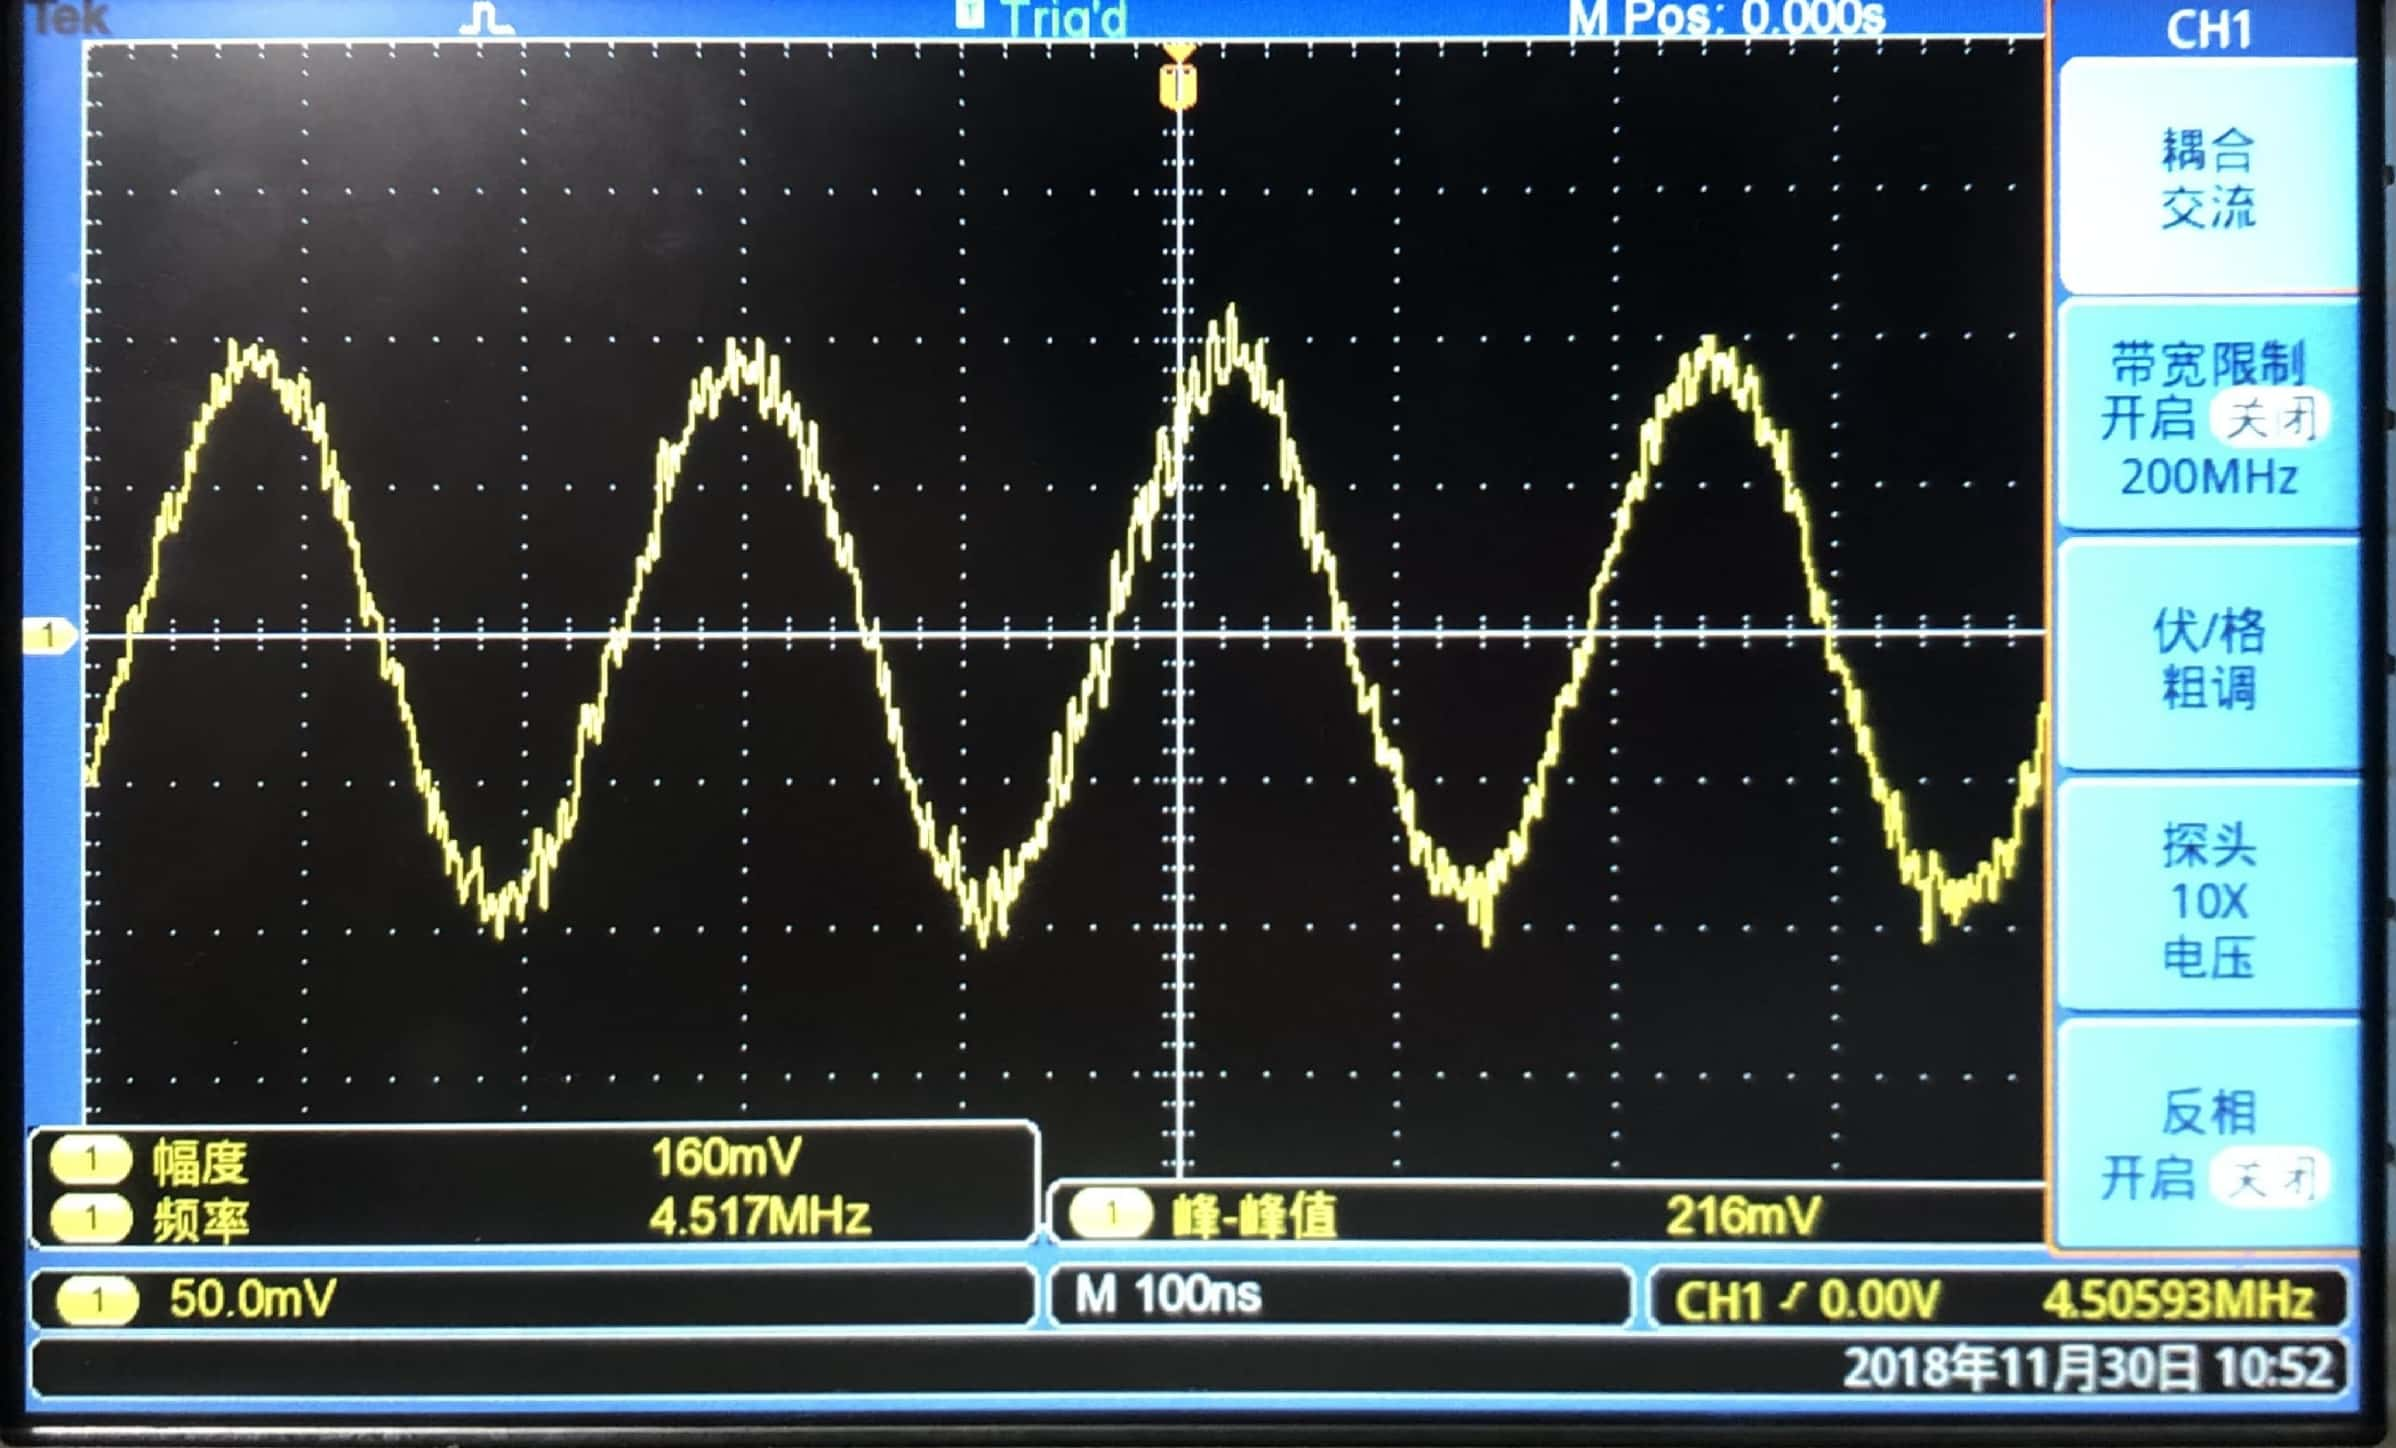
\includegraphics[width=0.35\textwidth]{gaopin3/gaopin321.jpg}   \\ \hline
300            & 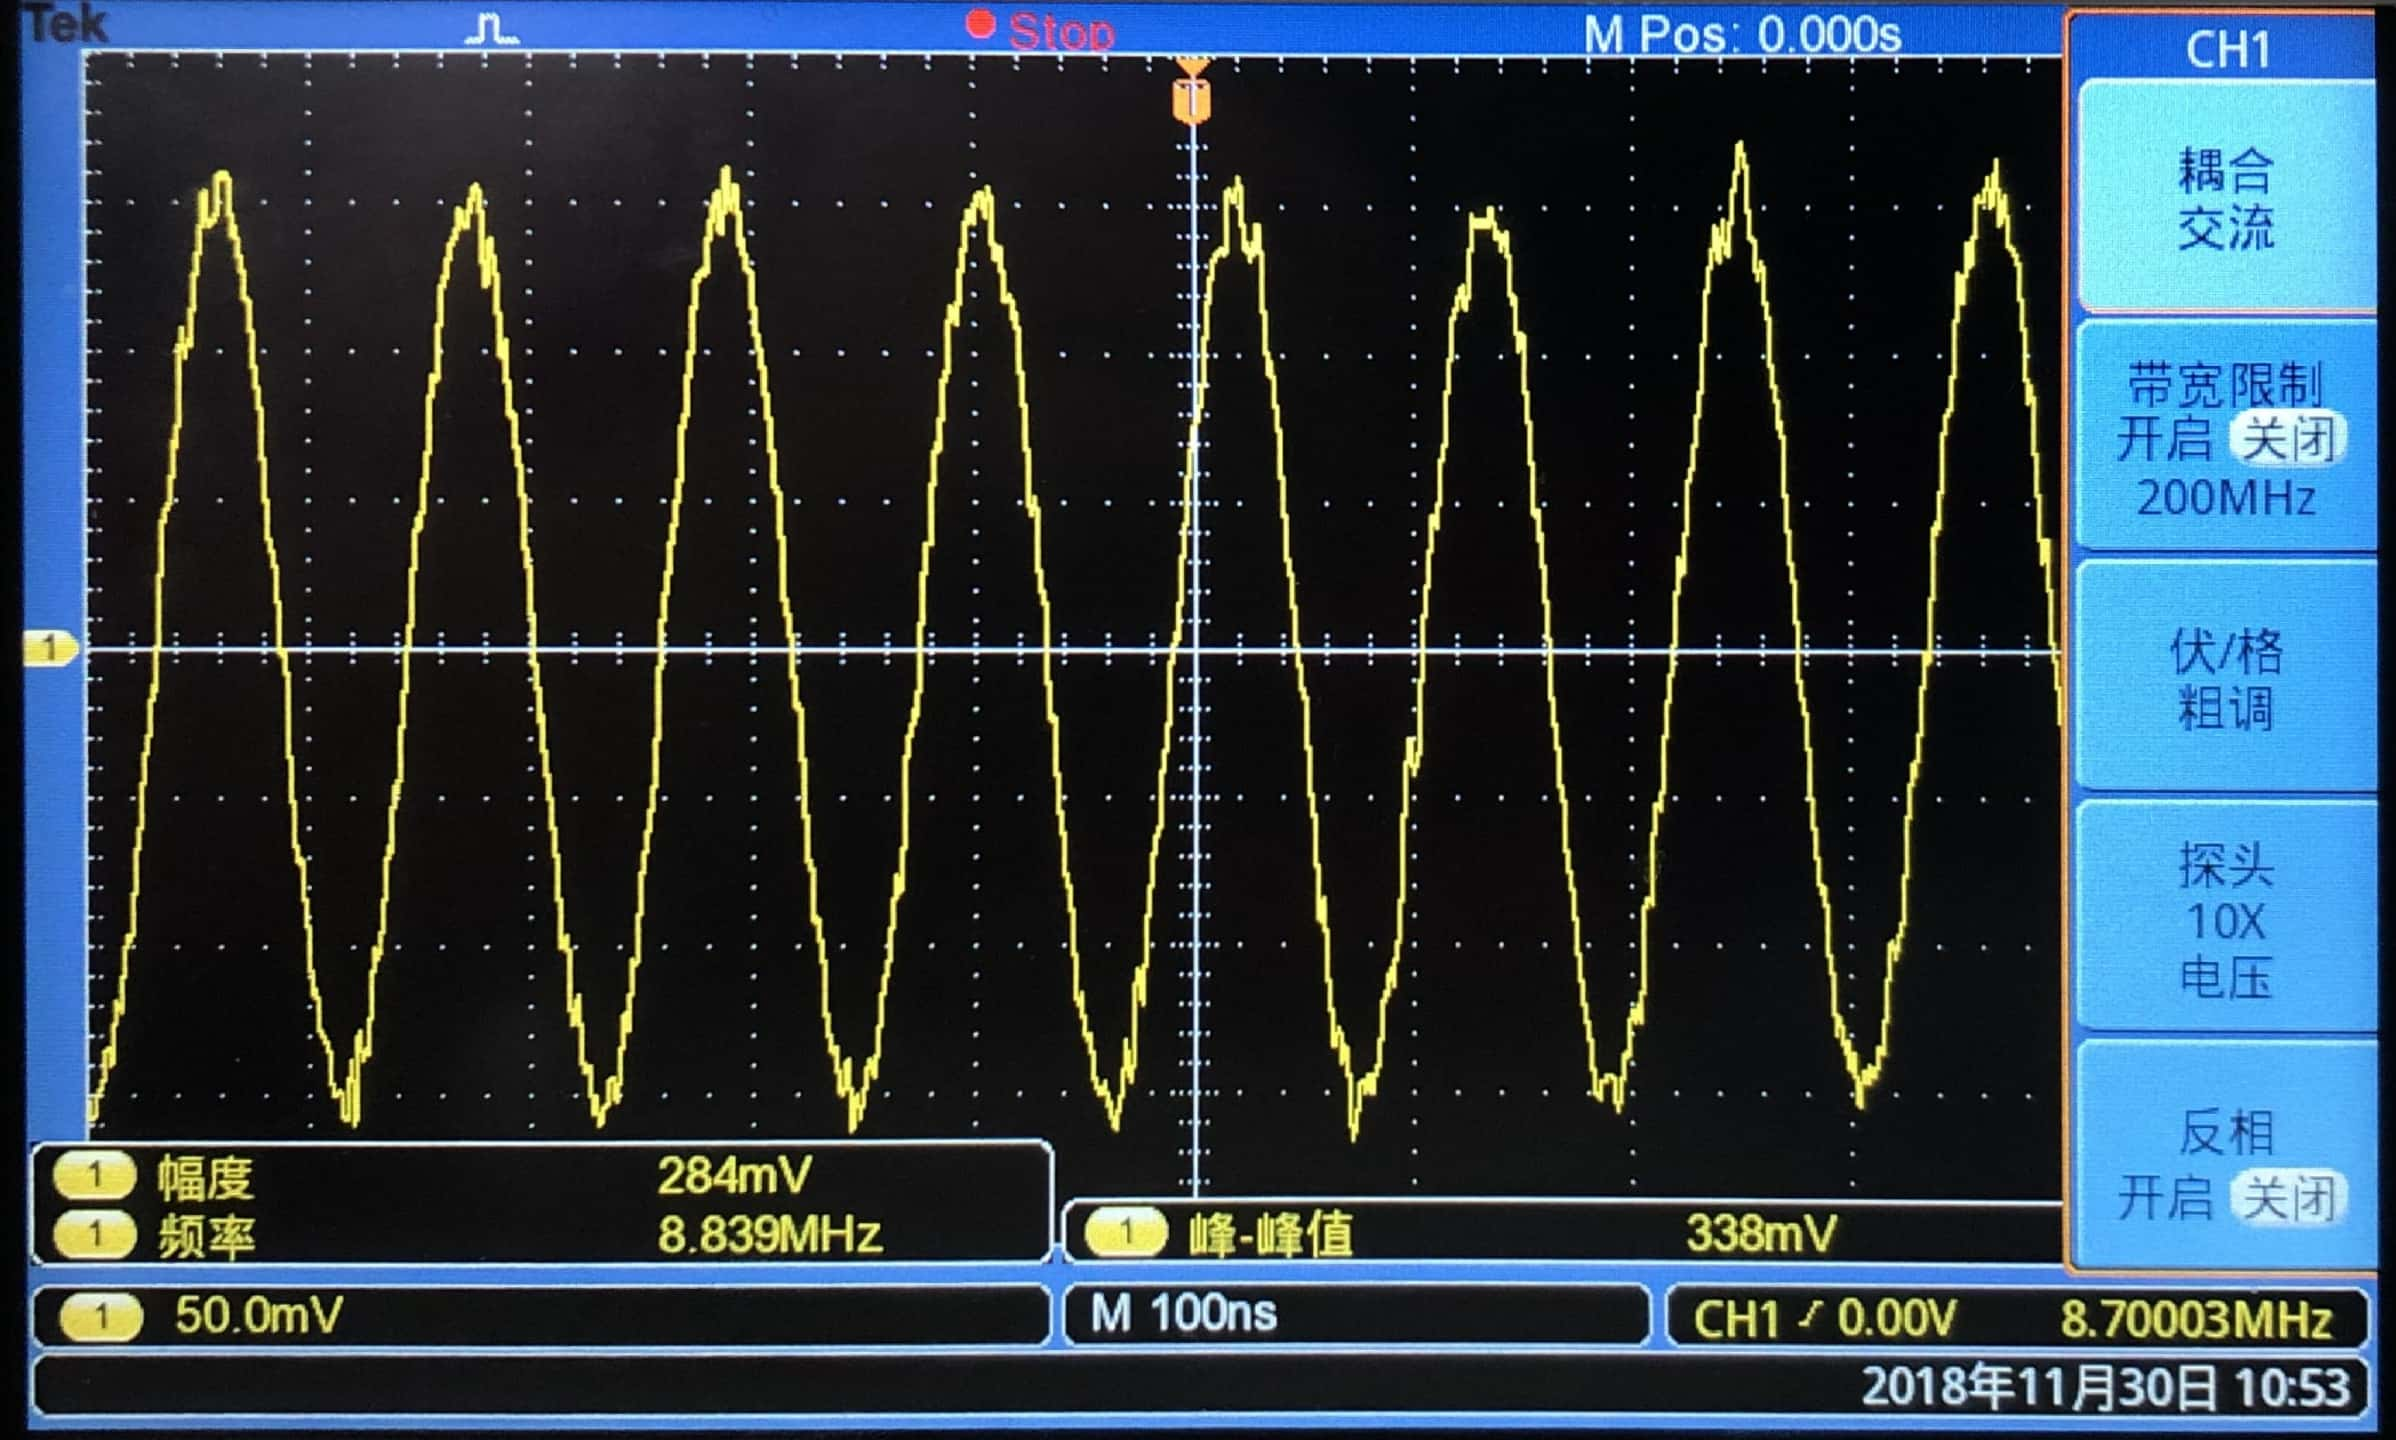
\includegraphics[width=0.35\textwidth]{gaopin3/gaopin305.jpg}   & 366            &  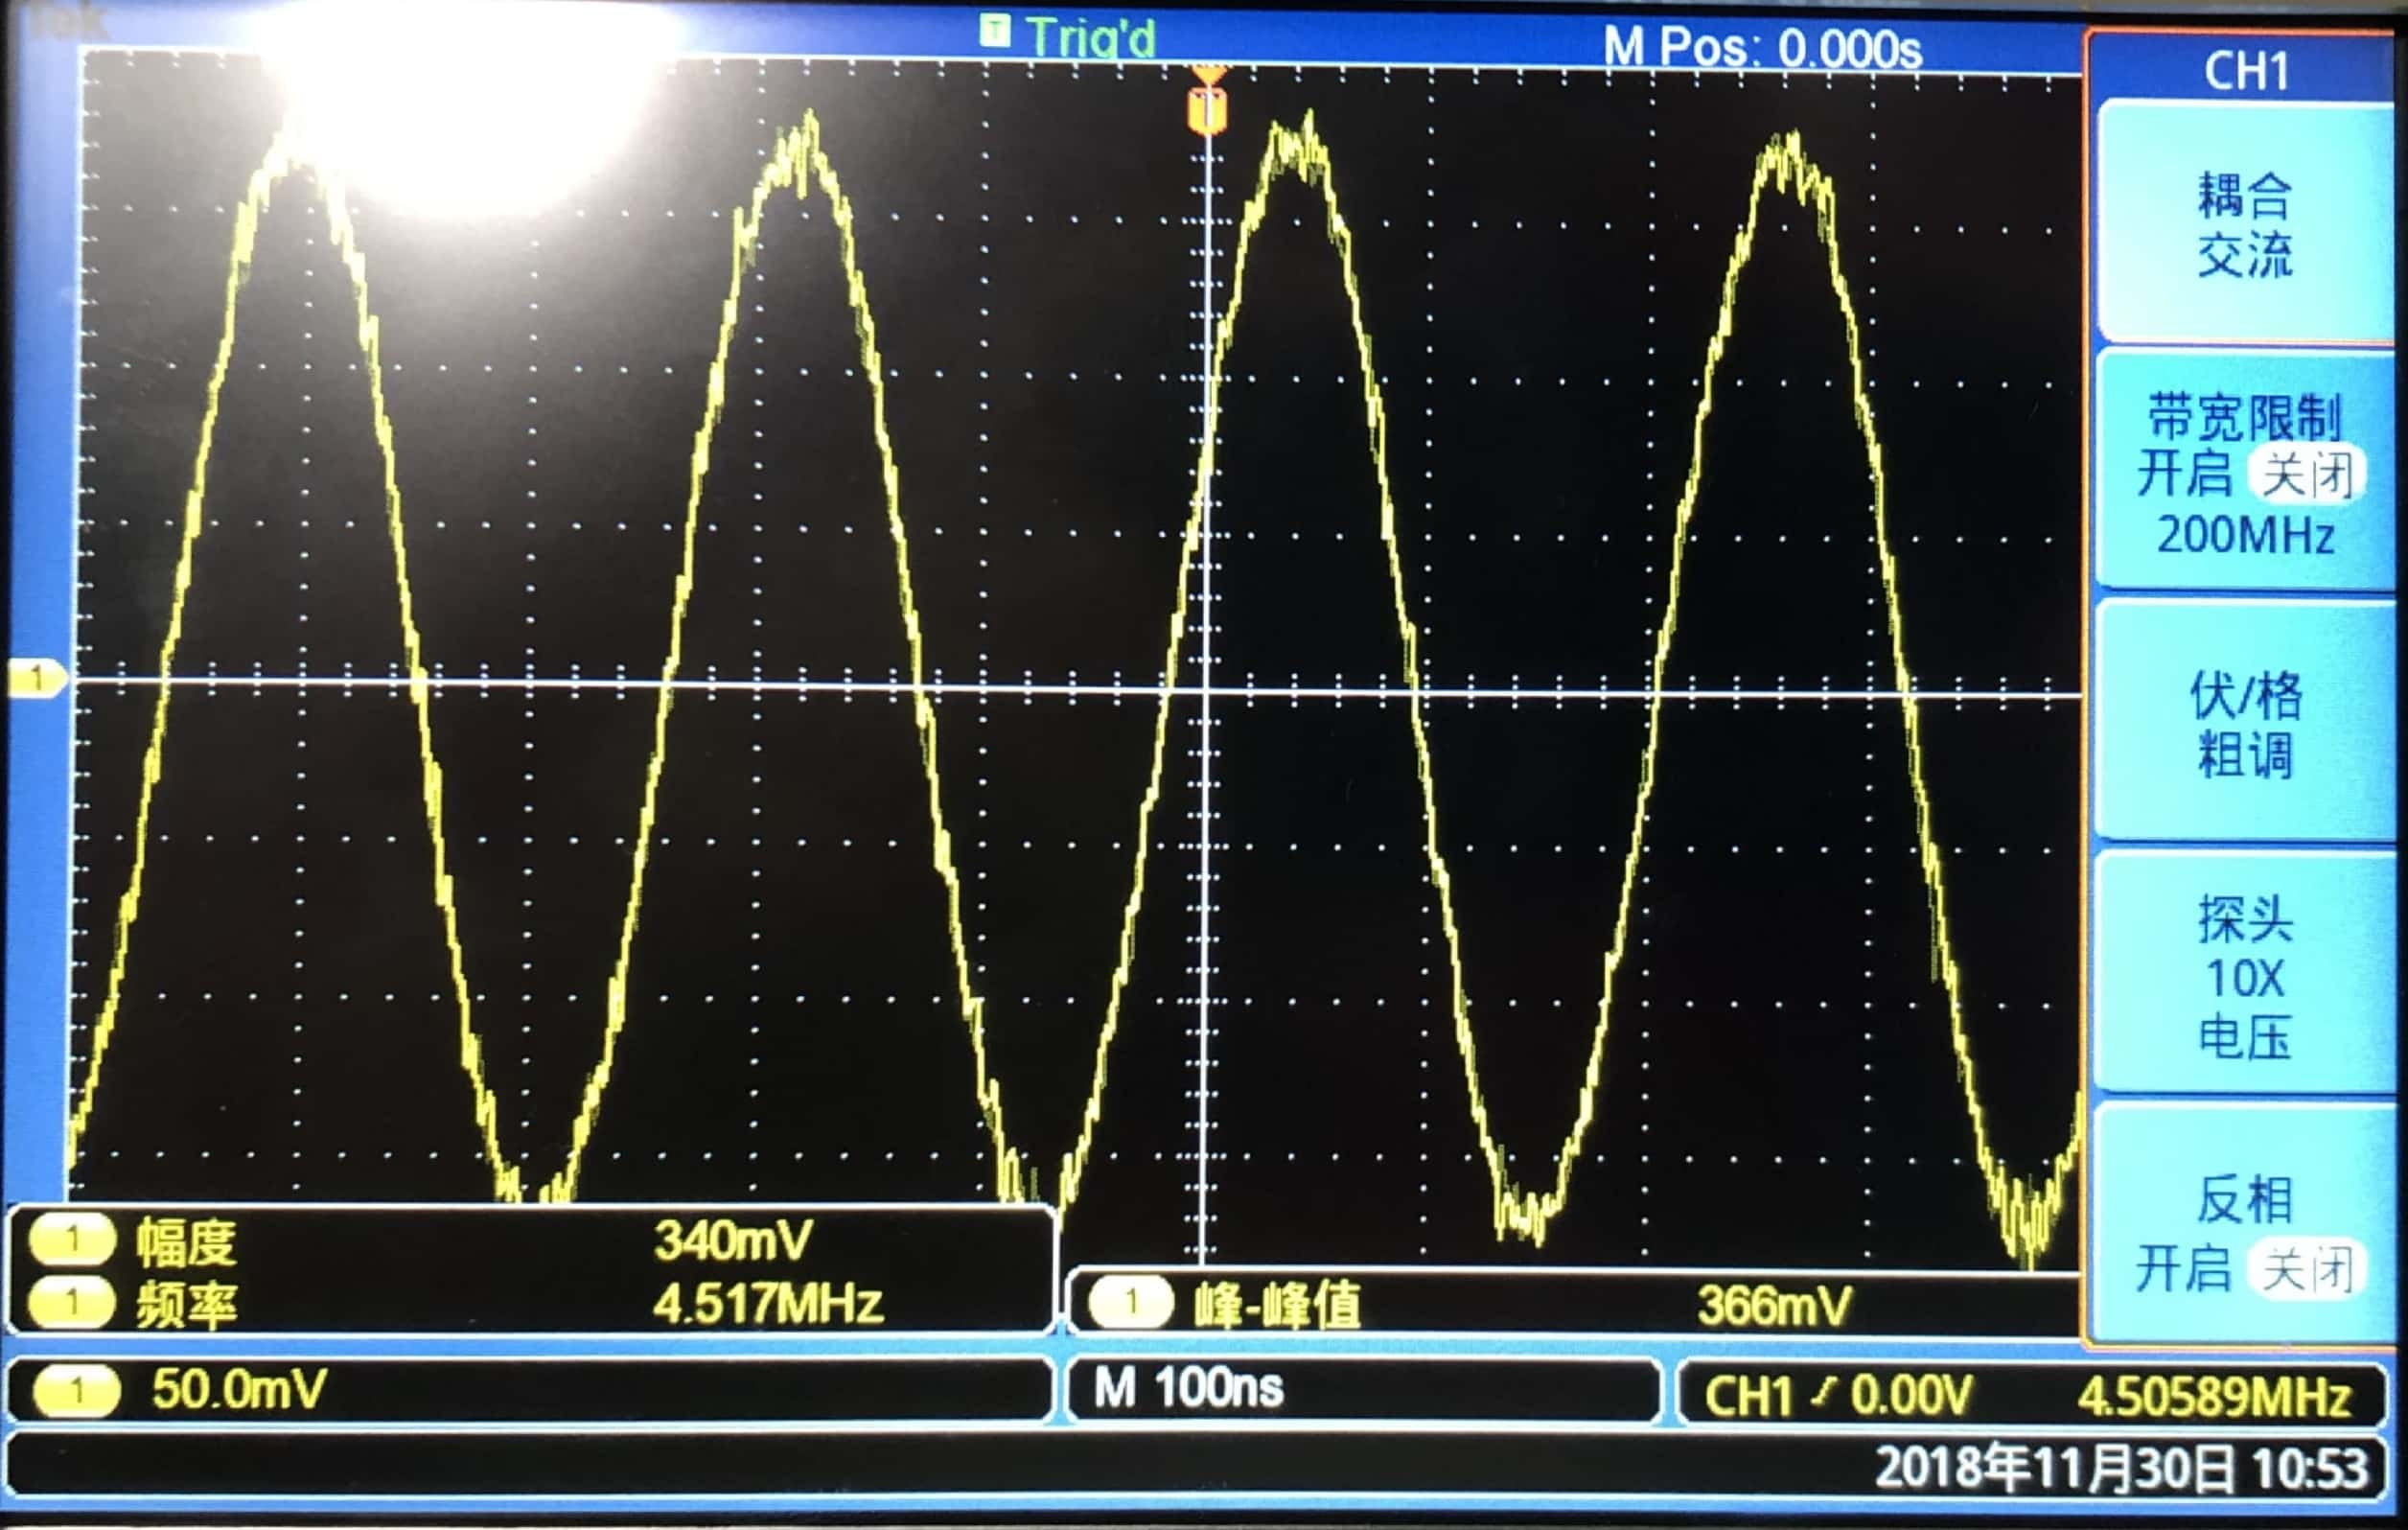
\includegraphics[width=0.35\textwidth]{gaopin3/gaopin308.jpg}  \\ \hline
400            &  \includegraphics[width=0.35\textwidth]{gaopin3/gaopin312.jpg}  & 452            & \includegraphics[width=0.35\textwidth]{gaopin3/gaopin304.jpg}   \\ \hline
500            &   \includegraphics[width=0.35\textwidth]{gaopin3/gaopin307.jpg} & 508            &      \includegraphics[width=0.35\textwidth]{gaopin3/gaopin306.jpg}\\ \hline
600            &    \includegraphics[width=0.35\textwidth]{gaopin3/gaopin302.jpg}  & 528            & \includegraphics[width=0.35\textwidth]{gaopin3/gaopin303.jpg}   \\ \hline
\end{tabular}
\end{table}

\item 对于表\ref{tab:ajk},其对应的高频信号电压幅度在$150mv$(见图\ref{img:bzbx2}),其对应的波形情况见表\ref{tab:ajk3}。
       \begin{figure}[htbp]
  \centering
  \includegraphics[width=.4\textwidth]{gaopin3/gaopin310.jpg} 
  \caption{ 高频信号波形} 
  \label{img:bzbx2} 
\end{figure}

\item 由表\ref{tab:ajk}和表\ref{tab:ajk3}的输出中频电压波形情况,可知混频后的波形频率在5.5058MHz左右
\end{enumerate}
\section{非线性丙类功率放大器实验(模块3)}
\setcounter{equation}{0}
\setcounter{table}{0}
\setcounter{figure}{0}
\subsection{实验目的}
\begin{enumerate}\addtolength{\itemsep}{-1.5ex}
\item 了解丙类功率放大器的基本工作原理,掌握丙类放大器的调谐特性以及负载改变时的动态特性。
\item 了解高频功率放大器丙类工作的物理过程以及当激励信号变化对功率放大器工作状态的影响。
\item 比较甲类功率放大器与丙类功率放大器的特点、功率、效率。
\end{enumerate}
\subsection{实验原理}
非线性丙类功率放大器通常作为发射机末级功放以获得较大的输出功率和较高的效率。特点:非线性丙类功率放大器通常用来放大窄带高频信号(信号的通带宽度只有其中心频率的1\%或更小),基极偏置为负值,电流导通角$\theta<90^o$,为了不失真地放大信号,它的负载必须是LC谐振回路。\par
电路原理图如图\ref{img:bl}所示,该实验电路由两级功率放大器组成。其中$Q_3$$(3D$$G$$12)$、$T_6$组成甲类功率放大器,工作在线性放大状态,其中$R_{A3},R_{14},R_{15}$组成静态偏置电阻,调节$R_{A3}$可改变放大器的增益。$W_1$为可调电阻,调节$W_1$可以改变输入信号幅度,$Q_4(3DG12)$、$T_4$组成丙类功率放大器。$R_{16}$为射极反馈电阻,$T_4$为谐振回路,甲类功放的输出信号通过$R_{13}$送到$Q_4$基极作为丙放的输入信号,此时只有当甲放输出信号大于丙放管$Q_4$基极-射极间的负偏压值时,$Q_4$才导通工作。与拨码开关相连的电阻为负载回路外接电阻,改变$S_1$拨码开关的位置可改变并联电阻值,即改变回路Q值。
\begin{figure}[htbp]
  \centering
  \includegraphics[width=\textwidth]{image015.png} 
  \caption{ 丙类功率放大器原理图} 
  \label{img:bl} 
\end{figure}
\subsection{实验步骤}
\subsubsection{测试调谐特性}
注;做实验之前请将S4开关拨下。\par
在前置放大电路出入J3口处输入频率$f=10.7MHz(V_{p-p}\approx880mV)$的高频信号,调节W1和中周T6,使TP6处信号的电压幅值至最大不失真,S1 至S3全部拨下,改变输入信号频率,从9MHz~15MHz(以1MHz为步进)记录TP6处的输出电压值,填入表\ref{tab:shuangfeng}。
\begin{table}[htbp]
\centering
\caption{调谐特性表}\label{tab:shuangfeng}
\begin{tabular}{|c|c|c|c|c|c|c|c|}
\hline
$f_i$    & 9MHz & 10MHz & 11MHz & 12MHz & 13MHz & 14MHz & 15MHz \\\hline
$V_0(V)$ & 2.12 & 2.60  & 3.96  & 3.04  & 2.88  & 2.32  & 1.68 \\\hline
\end{tabular}
\end{table}
\subsubsection{测试负载特性}
在前置放大电路中输入J3口处输入频率f=10.7MHz(Vp-p≈880mV)左右的高频信号,调节W1使TP6处信号约为3.2V左右,调节中周使回路调谐(调谐标准:TH4处波形为对称双峰)。\par
将负载电阻转换开关S1依次从1—3拨动,用示波器观测相应的Vc值和Ve波形,分析负载对工作状态的影响。

\begin{table}[htbp]
\centering
\caption{负载特性表}
\label{tab:fuzaitexing}
\begin{tabular}{|c|c|c|c|c|}
\hline
$RL(\Omega)$ & $V_{cP-P}(V)$ &$V_{cP-P}$波形& $V_e$ 波形 \\\hline
820          &        10.0       &  \includegraphics[width=0.35\textwidth]{gaopin4/gaopin422.jpg}   &  \includegraphics[width=0.35\textwidth]{gaopin4/gaopin418.jpg}   \\\hline
330          &         9.84      &   \includegraphics[width=0.35\textwidth]{gaopin4/gaopin421.jpg}  &   \includegraphics[width=0.35\textwidth]{gaopin4/gaopin419.jpg}  \\\hline
100          &          7.04     &    \includegraphics[width=0.35\textwidth]{gaopin4/gaopin420.jpg} &    \includegraphics[width=0.35\textwidth]{gaopin4/gaopin416.jpg}  \\\hline
$\infty$     &    10.3       &  \includegraphics[width=0.35\textwidth]{gaopin4/gaopin417.jpg} &   \includegraphics[width=0.35\textwidth]{gaopin4/gaopin415.jpg}   \\\hline
\end{tabular}
\end{table}
\subsection{实验仪器}
\begin{tabular}{clcc}
1.&	高频实验箱                &&        1台 \\
2.&	双踪示波器           &&             1台\\
3.&	万用表           &&             1块\\
\end{tabular}
\subsection{实验结果}
\begin{enumerate}\addtolength{\itemsep}{-1.5ex}
\item 对于测试调谐特性实验而言,由示波器测得的的初始输入信号波形如图\ref{img:shuru},此时调节中周后对应的最大幅度为2.96V,波形见图\ref{img:shuchu}。
\begin{figure}[htbp]
  \centering
  \includegraphics[width=.4\textwidth]{gaopin4/gaopin401.jpg} 
  \caption{ 初始输入波形} 
  \label{img:shuru} 
\end{figure}
\begin{figure}[htbp]
  \centering
  \includegraphics[width=.4\textwidth]{gaopin4/gaopin407.jpg} 
  \caption{ 最大幅度波形} 
  \label{img:shuchu} 
\end{figure}
\item 调谐特性表\ref{tab:shuangfeng}对应的波形情况见图\ref{fig:bili2}。
\begin{figure}[htbp]
\centering
\begin{tabular}{cc}
\includegraphics[width=0.4\textwidth]{gaopin4/gaopin409.jpg}&\includegraphics[width=0.4\textwidth]{gaopin4/gaopin408.jpg}\\
$f_i=9MHz$&$f_i=10MHz$\\
$V_0=2.12V$&$V_0=2.60V$\\
\includegraphics[width=0.4\textwidth]{gaopin4/gaopin410.jpg}&\includegraphics[width=0.4\textwidth]{gaopin4/gaopin413.jpg}\\
$f_i=11MHz$&$f_i=12MHz$\\
$V_0=3.96V$&$V_0=3.04V$\\
\includegraphics[width=0.4\textwidth]{gaopin4/gaopin412.jpg}&\includegraphics[width=0.4\textwidth]{gaopin4/gaopin411.jpg}\\
$f_i=13MHz$&$f_i=14MHz$\\
$V_0=2.88V$&$V_0=2.32V$\\
\multicolumn{2}{c}{\includegraphics[width=0.4\textwidth]{gaopin4/gaopin414.jpg}}\\
\multicolumn{2}{c}{$f_i=15MHz$}\\
\multicolumn{2}{c}{$V_0=1.68V$}\\
\end{tabular}
\caption{调谐特性波形图}
\label{fig:bili2}
\end{figure}
\item 负载特性表及波形情况见表\ref{tab:fuzaitexing}
\item \emph{对实验参数和波形进行分析,说明输入激励电压、负载电阻对工作状态的影响。}\par根据实验波形可以得出当负载慢由大变小时,输出波形依次经历过压状态 、临界状态与欠压状态。\par
当电阻为无穷大或 820$\Omega$时,输出波形呈过压状态,$V_e$为双峰, 电阻由 电阻由 820$\Omega$过渡至 300 $\Omega$时,过压状态逐渐呈减小状态,直至电阻达到100$\Omega$时已超越临界状态达到欠压,此时 $V_e$输出波形为单峰。\par
由实验数据可得, 在欠压与临界状态下,输出电压峰值随负载的增大而增大。
\end{enumerate}
\section{模拟乘法器调幅及同步检波实验(AM、DSB、SSB)(模块5)}
\setcounter{equation}{0}
\setcounter{table}{0}
\setcounter{figure}{0}
\subsection{实验目的}
\begin{enumerate}\addtolength{\itemsep}{-1.5ex}
\item 掌握用集成模拟乘法器实现全载波调幅、抑止载波双边带调幅和单边带调幅的方法。
\item研究已调波与调制信号以及载波信号的关系。
\item掌握调幅系数的测量与计算方法。
\item通过实验对比全载波调幅、抑止载波双边带调幅和单边带调幅的波形。
\end{enumerate}
\subsection{实验原理}
幅度调制就是载波的振幅(包络)随调制信号的参数变化而变化。本实验中载波是由高频信号源产生的465KHz高频信号,10KHz的低频信号为调制信号。振幅调制器即为产生调幅信号的装置。\par
用MC1496集成电路构成的调幅器电路图如图\ref{img:AM}所示。\par
       \begin{figure}[htbp]
  \centering
  \includegraphics[width=\textwidth]{image017.png} 
  \caption{ 调幅器电路图} 
  \label{img:AM} 
\end{figure}
图中W1用来调节引出脚1、4之间的平衡,器件采用双电源方式供电(+12V,-8V),所以5脚偏置电阻$R_{15}$接地。电阻$R_1,R_2,R_4,R_5,R_6$为器件提供静态偏置电压,保证器件内部的各个晶体管工作在放大状态。载波信号加在$V_1-V_4$的输入端,即引脚8、10之间;载波信号Vc经高频耦合电容$C_1$从10脚输入,$C_2$为高频旁路电容,使8脚交流接地。调制信号加在差动放大器$V_5,V_6$的输入端,即引脚1、4之间,调制信号$V_\Omega$经低频偶合电容$E_1$从1脚输入。2、3脚外接1K$\Omega$电阻,以扩大调制信号动态范围。当电阻增大,线性范围增大,但乘法器的增益随之减小。已调制信号取自双差动放大器的两集电极(即引出脚6、12之间)输出。
\subsection{实验步骤}
\subsubsection{全载波振幅调制}
 J1端输入载波信号$V_c(t) , f_c=465KHz, V_{CP-P}=500mV$,再从J5端口输入调制信号,其$f_\Omega=10KHz$,当$V_{\Omega P-P}$由零逐渐增大时,则输出信号$V_O(t)$的幅度发生变化,最后出现如图\ref{img:AMp}所示的有载波调幅信号的波形,记下AM波对应$V_{mmax}$和$V_mmin$,并计算调幅度$m=\frac{V_{m\ max}-V_{m\ min}}{V_{m\ max}+V_{m\ min}}$。
       \begin{figure}[htbp]
  \centering
  \includegraphics[width=.5\textwidth]{image019.png} 
  \caption{ 普通调幅波波形} 
  \label{img:AMp} 
\end{figure}
\subsubsection{集成电路(乘法器)构成解调器,解调全载波信号}
在保持调幅波输出的基础上,将调幅波和高频载波输入解调乘法器(见图\ref{img:jAM})J11和 J8端,用示波器观测解调器的输出,记录其频率和幅度。
       \begin{figure}[htbp]
  \centering
  \includegraphics[width=\textwidth]{image020.png} 
  \caption{解调器电路图 } 
  \label{img:jAM} 
\end{figure}

\subsection{实验仪器}
\begin{tabular}{clcc}
1.&	高频实验箱                &&        1台 \\
2.&	双踪示波器           &&             1台\\
3.&	万用表           &&             1块\\
\end{tabular}
\subsection{实验结果}
\begin{enumerate}\addtolength{\itemsep}{-1.5ex}
\item 由示波器测得的(信号源发生的)载波信号波形如图\ref{img:zbAM}所示。
 \begin{figure}[htbp]
  \centering
  \includegraphics[width=.5\textwidth]{gaopin5/gaopin506.jpg} 
  \caption{高频载波信号 } 
  \label{img:zbAM} 
\end{figure}
\item \emph{画出调幅实验中$m=30\%,m=50\%,m = 80\% $的调幅波形,分析过调幅的原因。}\par
经分析,调幅度m与调幅波调制信号最大值$V_{m\ max}$最小值$V_{m\ min}$比例关系见表\ref{tab:bili}。
\begin{table}[htbp]
\centering
\caption{调幅度与调制信号最大最小值比例关系表}
\label{tab:bili}
\begin{tabular}{|c|c|}
\hline
$m  $  & ${V_{m\    min}}/{V_{m\  max}}$ \\\hline
30\% & ${7}/{13}$                                                                \\\hline
50\% &$ {1}/{3}            $                                                     \\\hline
80\% & ${1}/{9}          $          \\\hline
\end{tabular}
\end{table}\par\par 则对应的大致波形如图\ref{fig:bili}所示
\begin{figure}[htbp]
\centering
\begin{tabular}{cc}
\includegraphics[width=0.45\textwidth]{gaopin5/gaopin502.jpg}&\includegraphics[width=0.45\textwidth]{gaopin5/gaopin504.jpg}\\
$m=30\%$&$m=50\%$\\
${V_{m\    min}}/{V_{m\  max}}={7}/{13}$&${V_{m\    min}}/{V_{m\  max}}= {1}/{3}    $\\
&\\
\multicolumn{2}{c}{\includegraphics[width=0.45\textwidth]{gaopin5/gaopin507.jpg}}\\
\multicolumn{2}{c}{$m=80\%$}\\
\multicolumn{2}{c}{${V_{m\    min}}/{V_{m\  max}}= {1}/{9}    $}\\
\end{tabular}
\caption{调幅波形图}
\label{fig:bili}
\end{figure}
\par\textbf{过调幅 原因:}\ 调制 波存在 小于0的幅度, 使得 载波 相乘 时, 小于0的部分 会被 翻到y轴正半轴, 产生 失真。
\item \emph{画出全载波调幅波解调后的波形。}\par全载波信号解调后的波形如图\ref{img:jjAM}。
\item 将解调后的波形连接到频率计上,由图\ref{fig:plj}可知,解调后的波形频率在10KHz左右,与原调制信号的频率大致相同。
 \begin{figure}[htbp]
  \centering
  \includegraphics[width=.5\textwidth]{gaopin5/gaopin505.jpg} 
  \caption{全载波调幅波解调波形 } 
  \label{img:jjAM} 
\end{figure}
 \begin{figure}[htbp]
  \centering
  \includegraphics[width=\textwidth]{gaopin5/gaopin501.jpg} \\\ \\
   \includegraphics[width=\textwidth]{gaopin5/gaopin503.jpg} 
  \caption{频率计 } 
  \label{fig:plj} 
\end{figure}
\end{enumerate}

\titleformat{\section}{\centering\heiti\zihao{4}}{综合实验}{0.3em}{}
\section{半双工调频无线对讲机}
\setcounter{equation}{0}
\setcounter{table}{0}
\setcounter{figure}{0}
\subsection{实验目的}
\begin{enumerate}\addtolength{\itemsep}{-1.5ex}
\item 在模块实验的基础上掌握调频发射机、接收机,整机组成原理,建立调频系统概念。
\item 掌握系统联调的方法,培养解决实际问题的能力。
\end{enumerate}
\subsection{实验内容}
\begin{enumerate}\addtolength{\itemsep}{-1.5ex}
\item 完成调频发射机整机联调。
\item 完成调频接收机整机联调。
\item 进行调频发送与接收系统联调。
\end{enumerate}
\subsection{实验电路说明}
该调频发射、接收机组成原理框图如图\ref{img:FM}所示,发射机由音频信号发生器,音频放大,调频、上变频、功放等电路组成。接收机则由高放,下变频、中频放大、限幅、FM解调、音频功放、耳机等部分组成。
       \begin{figure}[htbp]
  \centering
  \includegraphics[width=\textwidth]{image003.png} 
  \caption{ 半双工调频无线对讲机系统框图} 
  \label{img:FM} 
\end{figure}
\subsection{实验步骤}
\subsubsection{FM发射机实验}\label{yl:section}
原理:发信电路包括音频发生器、音频放大、调频、上变频与发射功放等电路组成。\par
首先由模块一产生所需发射的音频信号。经过音频放大器将其放大,调频至 12.5MHz后,经过高频放大器进行信号放大,最后由天线发射出去。 \par
\begin{enumerate}[1.]\addtolength{\itemsep}{-1.5ex}
\item 将模块1的S6拨上,即选通音乐信号,经$U_4$放大从J5口输出,调节W 3使J5口处信号为最大不失真状态,波形见图\ref{fig:f1}。
 \begin{figure}[htbp]
  \centering
  \includegraphics[width=.45\textwidth]{gaopin6/gaopin603.jpg}
  \caption{选通音乐信号 } 
  \label{fig:f1} 
\end{figure}
\item 将模块1的J5口通过开关S5切换连接到模块1的J2口,TH2处测试音乐信号,波形见图\ref{fig:f2}。
将模块1的S1、S3均拨上,调节CC1使J1端输出频率接近4.5MHz的调频信号(可在TH1处观测),波形见图\ref{fig:f3},调节W2和中周T1使波形达到最大不失真状态。
 \begin{figure}[htbp]
  \centering
  \includegraphics[width=.45\textwidth]{gaopin6/gaopin608.jpg}
  \caption{$TH_2$处音乐信号 } 
  \label{fig:f2} 
\end{figure}
 \begin{figure}[htbp]
  \centering
  \includegraphics[width=.45\textwidth]{gaopin6/gaopin604.jpg}
  \caption{$TH_1$处调频信号 } 
  \label{fig:f3} 
\end{figure}
\item 将模块1的J1连接到模块2的J6,另将信号源频率8MHz (VP-P≈500mV)的信号(由示波器测得的波形见图\ref{fig:f4})从模块2的J7口输入,经平衡混频可得到12.5MHz左右的高频信号(可在TH9处观测,波形见图\ref{fig:f5} )。\uline{混频原理参见前文\ref{yl:hunpin}内容}。
 \begin{figure}[htbp]
  \centering
  \includegraphics[width=.45\textwidth]{gaopin6/gaopin611.jpg}
  \caption{信号源产生的信号 } 
  \label{fig:f4} 
\end{figure}
 \begin{figure}[htbp]
  \centering
  \includegraphics[width=.45\textwidth]{gaopin6/gaopin606.jpg}
  \caption{上混频后的高频调频信号 } 
  \label{fig:f5} 
\end{figure}
\item\label{yl:gf} 将模块2的J8口连到模块3的J3口,从TH5可观测到放大后的12.5MHz高频信号,波形如图\ref{fig:f6}。,将已放大的高频信号从模块3的S4切换拨上送到天线发送出去。\par\uline{功率放大器原理:功率放大器是由晶体管与选频回路两部分组成。对高频小信号有放大 和选频作用。本实验中输入信号的频率$f_S=12.5MHz$。基极偏置电阻与射极电阻决定晶体管的静态工作点。可通过静态工作点改变放大器的增益。}\par\uline{放大器的调谐回路谐振时所对应频率$f_0$称为放大器的谐振频率,$f_0$的表达式为 :}
\begin{equation}
f_0=\frac{1}{2\pi\sqrt{LC_{\Sigma }}}
\end{equation}\uline{其中,$L$为调谐回路电感线圈的电感;$C_{\Sigma}$为调谐回路的总电容, 其表达式为 }\begin{equation}
C_{\Sigma}=C+P_1^2C_{oe}+P_2^2C_{ie}
\end{equation}\uline{$C_{oe}$为晶体管的输出电容; $C_{ie}$为晶体管的输入电容; $P_1$为初级线圈抽头系数;$ P_2$为次级线圈抽头系数。}\par\uline{放大器的谐振回路时,所对应电压倍数数 $A_{V0}$称为调谐放大器的电压放大倍数。 其表达式为}\begin{equation}
A_{V0}=\frac{v_o}{v_i}=\frac{-p_1p_2y_{fe}}{G+P_1^2g_{oe}+P_2^2g_{ie}}
\end{equation}

 \begin{figure}[htbp]
  \centering
  \includegraphics[width=.45\textwidth]{gaopin6/gaopin607.jpg}
  \caption{放大后的高频调频信号 } 
  \label{fig:f6} 
\end{figure}
\end{enumerate}
\subsubsection{FM接收机实验}
原理:收信电路包括高放、下变频、中频放大,限幅、FM 解调、音频功放等部分。\par
收信时,先由高频放大天线接收信号,再进行混频由12.5MHz 调频至4.5MHz,
产生中频信号;经过中频放大器后,送入鉴频器进行解调,解调出音频信号。最终音频信号由音频功率放大器放大后发出声响。
\begin{enumerate}[1.]\addtolength{\itemsep}{-1.5ex}
\item 将模块1天线接收到的信号通过S7开关切换送入到模块1的J3,从TH4处可观测到放大后的天线接收到的信号,波形见图\ref{fig:f7},将放大的高频信号从模块1的J4连接到模块2的J3,将信号源频率为8MHz的本振信号(约500mv左右,由示波器测得的波形见图\ref{fig:f4})从模块2的J4输入,调整本振频率使得混频输出为4.5M的中频信号(可在TH6处观测,波形间图\ref{fig:f11})。\par\uline{混频原理参见前文\ref{yl:hunpin}内容。}
 \begin{figure}[htbp]
  \centering
  \includegraphics[width=.45\textwidth]{gaopin6/gaopin609.jpg}
  \caption{天线接收到的信号 } 
  \label{fig:f7} 
\end{figure}
 \begin{figure}[htbp]
  \centering
  \includegraphics[width=.45\textwidth]{gaopin6/gaopin610.jpg}
  \caption{$TH_6$处中频信号 } 
  \label{fig:f11} 
\end{figure}
\item 将混频后的信号从J5处送入模块2的J1端口,可在TH3处观测到经选频放大后的4.5MHz中频信号,波形见图\ref{fig:f8},放大后的中频信号从模块2的J2口输出。\par\uline{功率放大器原理见上文\ref{yl:section}:\ref{yl:gf}内容。}
 \begin{figure}[htbp]
  \centering
  \includegraphics[width=.45\textwidth]{gaopin6/gaopin602.jpg}
  \caption{$TH_3$处中频信号 } 
  \label{fig:f8} 
\end{figure}
\item 将模块2的J2连到模块4的正交鉴频的输入端J6,适当调节L1,可从TH7处观测到解调后的信号,波形见图\ref{fig:f9}。\par\uline{鉴频原理:鉴频的作用是从已调波中检出反映在频率变化上的调制信号。}\par\uline{
在调频接收机中,当等幅信号通过鉴频前各级电路时,因率特性不均匀而导致调频信号谱结构的变化,从造成调制信号的振幅发生变化。如果存在着干扰,还会进一步加剧这种振幅的变化。鉴频器解调信号时上述寄生调幅就会反映在输出解电压上,产生失真。因此一般必须在鉴频前加一限幅器以消除寄生调,保证到鉴频上的调频电压是等幅的。可见,限幅与鉴频一般是连用的,统称为限幅鉴频器。}
 \begin{figure}[htbp]
  \centering
  \includegraphics[width=.45\textwidth]{gaopin6/gaopin612.jpg}
  \caption{解调后的信号 } 
  \label{fig:f9} 
\end{figure}
\item 将模块4的J7连到模块4的J11,经放大后的信号从模块4的J12口连接到模块6的J6口输入到喇叭,可适当调节模块4的W1和模块4的L1,使耳机听到的声音音质清晰。
\end{enumerate}

\subsection{实验仪器}
\begin{tabular}{clcc}
1.&	高频实验箱                &&        1台 \\
2.&	双踪示波器           &&             1台\\
\end{tabular}
\subsection{调试中遇到的问题及分析}
\begin{enumerate}[1.]\addtolength{\itemsep}{-1.5ex}
\item 由于模块2的多个接口松动,导致混频接触不良,时好时坏。前期,我们没有发现问题的出处,在排查问题时忽略了这一点,致使通电时间过长,烧坏了模块3的丙类放大器。在更换了模块3后,仍然无法听到音频,才发现了模块2问题的严重性。拆下模块2并拧紧接触部件的螺母后,混频器可以稳定地工作了。
\item 在解决以上问题后,可以听到极为微弱的声音,调节模块4的W1、L1也无法得到良好的效果,噪声仍然很大。后来发现是因为信号通过天线的传播衰减过大,将两个天线的发射、接收部分直接接触,声音效果得到一定的改善。
\end{enumerate}
\end{document}
